%%%%%%%%%%%%%%%%%%%%%%%%%%%%% Thesis.tex %%%%%%%%%%%%%%%%%%%%%%%%%%%%%%%
%                                                                      %
%  ---------- Master of Science Dissertation template ----------       %
%                                                                      %
%  Template for the Master Thesis according to the regulations         %
%  published by the Academic Board (Direcção Académica) at IST.        %
%                                                                      %
%  For up-to-date guide, please refer to the official website          %
%  http://academica.tecnico.ulisboa.pt/alunos/dissertacao-de-mestrado/ %
%                                                                      %
%       Andre C. Marta                                                 %
%       Area Cientifica de Mecanica Aplicada e Aeroespacial            %
%       Departamento de Engenharia Mecanica                            %
%       Instituto Superior Tecnico                                     %
%       Av. Rovisco Pais                                               %
%       1049-001 Lisboa                                                %
%       Portugal                                                       %
%       Tel: +351 21 841 9469                                          %
%                        3469 (extension)                              %
%       Email: andre.marta@tecnico.ulisboa.pt                          %
%                                                                      %
%  Created:       Jan 20, 2011                                         %
%  Last Modified: Feb 19, 2018                                         %
%                                                                      %
%%%%%%%%%%%%%%%%%%%%%%%%%%%%%%%%%%%%%%%%%%%%%%%%%%%%%%%%%%%%%%%%%%%%%%%%
%  Revision history                                                    %
%  v1 - 2011/01/24 - original template                                 %
%  v2 - 2012/10/30 - new IST image and  support                %
%  v3 - 2013/12/10 - update according to 2012/13 official guide        %
%  v4 - 2014/02/28 - new default for bibliography style                %
%  v5 - 2014/05/07 - update according to 2013/14 official guide        %
%  v6 - 2015/07/02 - cover page format fixed,                          %
%                    contents page numbering fixed,                    %
%                    better language support,                          %
%                    enhanced examples of tables,                      %
%                    new option for appendix page numbering format,    %
%                    custom bibliography style                         %
%  v7 - 2018/02/19 - multiple citations compressed                     %
%%%%%%%%%%%%%%%%%%%%%%%%%%%%%%%%%%%%%%%%%%%%%%%%%%%%%%%%%%%%%%%%%%%%%%%%
%                                                                      %
% To generate the PDF file, type "make" at the terminal prompt.        %
%                                                                      %
% The IST template LaTeX package was created by the author             %
% and it can be downloaded from:                                       %
% https://fenix.ist.utl.pt/homepage/ist31052/                          %
%                                                                      %
% The external packages can be downloaded from                         %
% the Comprehensive TeX Archive Network at http://www.ctan.org/        %
%                                                                      %
% List of LaTex symbols:                                               %
% http://www.ctan.org/tex-archive/info/symbols/comprehensive/          %
%                                                                      %
% Help with LaTex can be found at                                      %
% http://www.giss.nasa.gov/tools/latex/ltx-2.html                      %
% http://en.wikibooks.org/wiki/LaTeX                                   %
%%%%%%%%%%%%%%%%%%%%%%%%%%%%%%%%%%%%%%%%%%%%%%%%%%%%%%%%%%%%%%%%%%%%%%%%

%%%%%%%%%%%%%%%%%%%%%%%%%%%%%%%%%%%%%%%%%%%%%%%%%%%%%%%%%%%%%%%%%%%%%%%%
%     Preamble                                                         %
%%%%%%%%%%%%%%%%%%%%%%%%%%%%%%%%%%%%%%%%%%%%%%%%%%%%%%%%%%%%%%%%%%%%%%%%

% ----------------------------------------------------------------------
%  Set the document class
% ----------------------------------------------------------------------
\documentclass[10pt,a4paper,twoside]{report}

% ----------------------------------------------------------------------
% Define external packages, language, margins, fonts and new commands
% ----------------------------------------------------------------------
\usepackage{lineno}
\linenumbers
\usepackage{mathtools} 
\usepackage{wrapfig}
\usepackage[table,xcdraw]{xcolor}
\usepackage[utf8]{inputenc}
\usepackage{slashed}
\usepackage{multirow}
\usepackage{hhline}
\usepackage{tikz}
\usepackage[compat=1.1.0]{tikz-feynman}
\usepackage{diagbox}
%%%%%%%%%%%%%%%%%%%%%%%%%%%%%%%%%%%%%%%%%%%%%%%%%%%%%%%%%%%%%%%%%%%%%%%%
%                                                                      %
%     File: Thesis_Preamble.tex                                        %
%     Tex Master: Thesis.tex                                           %
%                                                                      %
%     Author: Andre C. Marta                                           %
%     Last modified : 9 Apr 2015                                       %
%                                                                      %
%%%%%%%%%%%%%%%%%%%%%%%%%%%%%%%%%%%%%%%%%%%%%%%%%%%%%%%%%%%%%%%%%%%%%%%%

% ----------------------------------------------------------------------
% Define document language.
% ----------------------------------------------------------------------

% 'inputenc' package
%
% Accept different input encodings.
% http://www.ctan.org/tex-archive/macros/latex/base/
%
% > allows typing non-english text in LaTeX sources.
%
% ******************************* SELECT *******************************
%\usepackage[latin1]{inputenc} % <<<<< Windows
\usepackage[utf8]{inputenc}   % <<<<< Linux
% ******************************* SELECT *******************************


% 'babel' package
%
% Multilingual support for Plain TeX or LaTeX.
% http://www.ctan.org/tex-archive/macros/latex/required/babel/
%
% > sets the variable names according to the language selected
%
% ******************************* SELECT *******************************
%\usepackage[portuguese]{babel} % <<<<< Portuguese
\usepackage[english]{babel} % <<<<< English
% ******************************* SELECT *******************************


% List of LaTeX variable names: \abstractname, \appendixname, \bibname,
%   \chaptername, \contentsname, \listfigurename, \listtablename, ...)
% http://www.tex.ac.uk/cgi-bin/texfaq2html?label=fixnam
%
% Changing the words babel uses (uncomment and redefine as necessary...)
%
\newcommand{\acknowledgments}{@undefined} % new LaTeX variable name
%
% > English
%
\addto\captionsenglish{\renewcommand{\acknowledgments}{Acknowledgments}}
%\addto\captionsenglish{\renewcommand{\contentsname}{Contents}}
%\addto\captionsenglish{\renewcommand{\listtablename}{List of Tables}}
%\addto\captionsenglish{\renewcommand{\listfigurename}{List of Figures}}
%\addto\captionsenglish{\renewcommand{\nomname}{Nomenclature}}
%\addto\captionsenglish{\renewcommand{\glossaryname}{Glossary}}
%\addto\captionsenglish{\renewcommand{\acronymname}{List of Acronyms}}
%\addto\captionsenglish{\renewcommand{\bibname}{References}} % Bibliography
%\addto\captionsenglish{\renewcommand{\appendixname}{Appendix}}

% > Portuguese
%
\addto\captionsportuguese{\renewcommand{\acknowledgments}{Agradecimentos}}
%\addto\captionsportuguese{\renewcommand{\contentsname}{Conte\'{u}do}}
%\addto\captionsportuguese{\renewcommand{\listtablename}{Lista de Figuras}}
%\addto\captionsportuguese{\renewcommand{\listfigurename}{Lista de Tabelas}}
\addto\captionsportuguese{\renewcommand{\nomname}{Lista de S\'{i}mbolos}} % Nomenclatura
%\addto\captionsportuguese{\renewcommand{\glossary}{Gloss\'{a}rio}}
%\addto\captionsportuguese{\renewcommand{\acronymname}{Lista de Abrevia\c{c}\~{o}es}}
%\addto\captionsportuguese{\renewcommand{\bibname}{Refer\^{e}ncias}} % Bibliografia
%\addto\captionsportuguese{\renewcommand{\appendixname}{Anexo}} % Apendice


% ----------------------------------------------------------------------
% Define cover fields in both english and portuguese.
% ----------------------------------------------------------------------
%
\newcommand{\coverThesis}{@undefined} % new LaTeX variable name
\newcommand{\coverSupervisors}{@undefined} % new LaTeX variable name
\newcommand{\coverExaminationCommittee}{@undefined} % new LaTeX variable name
\newcommand{\coverChairperson}{@undefined} % new LaTeX variable name
\newcommand{\coverSupervisor}{@undefined} % new LaTeX variable name
\newcommand{\coverMemberCommittee}{@undefined} % new LaTeX variable name
% > English
\addto\captionsenglish{\renewcommand{\coverThesis}{Thesis to obtain the Master of Science Degree in}}
\addto\captionsenglish{\renewcommand{\coverSupervisors}{Supervisor(s)}}
\addto\captionsenglish{\renewcommand{\coverExaminationCommittee}{Examination Committee}}
\addto\captionsenglish{\renewcommand{\coverChairperson}{Chairperson}}
\addto\captionsenglish{\renewcommand{\coverSupervisor}{Supervisor}}
\addto\captionsenglish{\renewcommand{\coverMemberCommittee}{Member of the Committee}}
% > Portuguese
\addto\captionsportuguese{\renewcommand{\coverThesis}{Disserta\c{c}\~{a}o para obten\c{c}\~{a}o do Grau de Mestre em}}
\addto\captionsportuguese{\renewcommand{\coverSupervisors}{Orientador(es)}}
\addto\captionsportuguese{\renewcommand{\coverExaminationCommittee}{J\'{u}ri}}
\addto\captionsportuguese{\renewcommand{\coverChairperson}{Presidente}}
\addto\captionsportuguese{\renewcommand{\coverSupervisor}{Orientador}}
\addto\captionsportuguese{\renewcommand{\coverMemberCommittee}{Vogal}}


% ----------------------------------------------------------------------
% Define default and cover page fonts.
% ----------------------------------------------------------------------

% Use Arial font as default
%
\renewcommand{\rmdefault}{phv}
\renewcommand{\sfdefault}{phv}

% Define cover page fonts
%
%         encoding     family       series      shape
%  \usefont{T1}     {phv}=helvetica  {b}=bold    {n}=normal
%                   {ptm}=times      {m}=normal  {sl}=slanted
%                                                {it}=italic
% see more examples at
% http://julien.coron.free.fr/languages/latex/fonts/
%
\def\FontLn{% 16 pt normal
  \usefont{T1}{phv}{m}{n}\fontsize{16pt}{16pt}\selectfont}
\def\FontLb{% 16 pt bold
  \usefont{T1}{phv}{b}{n}\fontsize{16pt}{16pt}\selectfont}
\def\FontMn{% 14 pt normal
  \usefont{T1}{phv}{m}{n}\fontsize{14pt}{14pt}\selectfont}
\def\FontMb{% 14 pt bold
  \usefont{T1}{phv}{b}{n}\fontsize{14pt}{14pt}\selectfont}
\def\FontSn{% 12 pt normal
  \usefont{T1}{phv}{m}{n}\fontsize{12pt}{12pt}\selectfont}


% ----------------------------------------------------------------------
% Define page margins and line spacing.
% ----------------------------------------------------------------------

% 'geometry' package
%
% Flexible and complete interface to document dimensions.
% http://www.ctan.org/tex-archive/macros/latex/contrib/geometry/
%
% > set the page margins (2.5cm minimum in every side, as per IST rules)
%
\usepackage{geometry}	
\geometry{verbose,tmargin=2.5cm,bmargin=2.5cm,lmargin=2.5cm,rmargin=2.5cm}

% 'setspace' package
%
% Set space between lines.
% http://www.ctan.org/tex-archive/macros/latex/contrib/setspace/
%
% > allow setting line spacing (line spacing of 1.5, as per IST rules)
%
\usepackage{setspace}
\renewcommand{\baselinestretch}{1.5}


% ----------------------------------------------------------------------
% Include external packages.
% Note that not all of these packages may be available on all system
% installations. If necessary, include the .sty files locally in
% the <jobname>.tex file directory.
% ----------------------------------------------------------------------

% 'graphicx' package
%
% Enhanced support for graphics.
% http://www.ctan.org/tex-archive/macros/latex/required/graphics/
%
% > extends arguments of the \includegraphics command
%
\usepackage{graphicx}


% 'color' package
%
% Colour control for LaTeX documents.
% http://www.ctan.org/tex-archive/macros/latex/required/graphics/
%
% > defines color macros: \color{<color name>}
%
%\usepackage{color}


% 'amsmath' package
%
% Mathematical enhancements for LaTeX.
% http://www.ctan.org/tex-archive/macros/latex/required/amslatex/
%
% > American Mathematical Society plain Tex macros
%
\usepackage{amsmath}  % AMS mathematical facilities for LaTeX.
\usepackage{amsthm}   % Typesetting theorems (AMS style).
\usepackage{amsfonts} % 


% 'wrapfig' package
%
% Produces figures which text can flow around.
% http://www.ctan.org/tex-archive/macros/latex/contrib/wrapfig/
%
% > wrap figures/tables in text (i.e., Di Vinci style)
%
% \usepackage{wrapfig}


% 'subfigure' package
%
% Deprecated: Figures divided into subfigures.
% http://www.ctan.org/tex-archive/obsolete/macros/latex/contrib/subfigure/
%
% > subcaptions for subfigures
%
\usepackage{subfigure}


% 'subfigmat' package
%
% Automates layout when using the subfigure package.
% http://www.ctan.org/tex-archive/macros/latex/contrib/subfigmat/
%
% > matrices of similar subfigures
%
\usepackage{subfigmat}


% 'url' package
%
% Verbatim with URL-sensitive line breaks.
% http://www.ctan.org/tex-archive/macros/latex/contrib/url/
%
% > URLs in BibTex
%
% \usepackage{url}


% 'varioref' package
%
% Intelligent page references.
% http://www.ctan.org/tex-archive/macros/latex/required/tools/
%
% > smart page, figure, table and equation referencing
%
%\usepackage{varioref}


% 'dcolumn' package
%
% Align on the decimal point of numbers in tabular columns.
% http://www.ctan.org/tex-archive/macros/latex/required/tools/
%
% > decimal-aligned tabular math columns
%
\usepackage{dcolumn}
\newcolumntype{d}{D{.}{.}{-1}} % column aligned by the point separator '.'
\newcolumntype{e}{D{E}{E}{-1}} % column aligned by the exponent 'E'


% 'verbatim' package
%
% Reimplementation of and extensions to LaTeX verbatim.
% http://www.ctan.org/tex-archive/macros/latex/required/tools/
%
% > provides the verbatim environment (\begin{verbatim},\end{verbatim})
%   and a comment environment (\begin{comment},  \end{comment})
%
% \usepackage{verbatim}


% 'moreverb' package
%
% Extended verbatim.
% http://www.ctan.org/tex-archive/macros/latex/contrib/moreverb/
%
% > supports tab expansion and line numbering
%
% \usepackage{moreverb}



% 'nomencl' package
%
% Produce lists of symbols as in nomenclature.
% http://www.ctan.org/tex-archive/macros/latex/contrib/nomencl/
%
% The nomencl package makes use of the MakeIndex program
% in order to produce the nomenclature list.
%
% Nomenclature
% 1) On running the file through LATEX, the command \makenomenclature
%    in the preamble instructs it to create/open the nomenclature file
%    <jobname>.nlo corresponding to the LATEX file <jobname>.tex and
%    writes the information from the \nomenclature commands to this file.
% 2) The next step is to invoke MakeIndex in order to produce the
%    <jobname>.nls file. This can be achieved by making use of the
%    command: makeindex <jobname>.nlo -s nomencl.ist -o <jobname>.nls
% 3) The last step is to invoke LATEX on the <jobname>.tex file once
%    more. There, the \printnomenclature in the document will input the
%    <jobname>.nls file and process it according to the given options.
%
% http://www-h.eng.cam.ac.uk/help/tpl/textprocessing/nomencl.pdf
%
% Nomenclature (produces *.nlo *.nls files)
\usepackage{nomencl}
\makenomenclature
%
% Group variables according to their symbol type
%
\RequirePackage{ifthen} 
\ifthenelse{\equal{\languagename}{english}}%
    { % English
    \renewcommand{\nomgroup}[1]{%
      \ifthenelse{\equal{#1}{R}}{%
        \item[\textbf{Roman symbols}]}{%
        \ifthenelse{\equal{#1}{G}}{%
          \item[\textbf{Greek symbols}]}{%
          \ifthenelse{\equal{#1}{S}}{%
            \item[\textbf{Subscripts}]}{%
            \ifthenelse{\equal{#1}{T}}{%
              \item[\textbf{Superscripts}]}{}}}}}%
    }{% Portuguese
    \renewcommand{\nomgroup}[1]{%
      \ifthenelse{\equal{#1}{R}}{%
        \item[\textbf{Simbolos romanos}]}{%
        \ifthenelse{\equal{#1}{G}}{%
          \item[\textbf{Simbolos gregos}]}{%
          \ifthenelse{\equal{#1}{S}}{%
            \item[\textbf{Subscritos}]}{%
            \ifthenelse{\equal{#1}{T}}{%
              \item[\textbf{Sobrescritos}]}{}}}}}%
    }%


% 'glossary' package
%
% Create a glossary.
% http://www.ctan.org/tex-archive/macros/latex/contrib/glossary/
%
% Glossary (produces *.glo *.ist files)
\usepackage[number=none]{glossary}
%\usepackage[acronym]{glossaries}
% (remove blank line between groups)
\setglossary{gloskip={}}
% (redefine glossary style file)
%\renewcommand{\istfilename}{myGlossaryStyle.ist}
\makeglossary


% 'rotating' package
%
% Rotation tools, including rotated full-page floats.
% http://www.ctan.org/tex-archive/macros/latex/contrib/rotating/
%
% > show wide figures and tables in landscape format:
%   use \begin{sidewaystable} and \begin{sidewaysfigure}
%   instead of 'table' and 'figure', respectively.
%
\usepackage{rotating}


% 'hyperref' package
%
% Extensive support for hypertext in LaTeX.
% http://www.ctan.org/tex-archive/macros/latex/contrib/hyperref/
%
% > Extends the functionality of all the LATEX cross-referencing
%   commands (including the table of contents, bibliographies etc) to
%   produce \special commands which a driver can turn into hypertext
%   links; Also provides new commands to allow the user to write adhoc
%   hypertext links, including those to external documents and URLs.
%
\usepackage[pdftex]{hyperref} % enhance documents that are to be
                              % output as HTML and PDF
\hypersetup{colorlinks,       % color text of links and anchors,
                              % eliminates borders around links
%            linkcolor=red,    % color for normal internal links
            linkcolor=black,  % color for normal internal links
            anchorcolor=black,% color for anchor text
%            citecolor=green,  % color for bibliographical citations
            citecolor=black,  % color for bibliographical citations
%            filecolor=magenta,% color for URLs which open local files
            filecolor=black,  % color for URLs which open local files
%            menucolor=red,    % color for Acrobat menu items
            menucolor=black,  % color for Acrobat menu items
%            pagecolor=red,    % color for links to other pages
            pagecolor=black,  % color for links to other pages
%            urlcolor=cyan,    % color for linked URLs
            urlcolor=black,   % color for linked URLs
	          bookmarks=true,         % create PDF bookmarks
	          bookmarksopen=false,    % don't expand bookmarks
	          bookmarksnumbered=true, % number bookmarks
	          pdftitle={Thesis},
            pdfauthor={Andre C. Marta},
            pdfsubject={Thesis Title},
            pdfkeywords={Thesis Keywords},
            pdfstartview=FitV,
            pdfdisplaydoctitle=true}


% 'hypcap' package
%
% Adjusting the anchors of captions.
% http://www.ctan.org/tex-archive/macros/latex/contrib/oberdiek/
%
% > fixes the problem with hyperref, that links to floats points
%   below the caption and not at the beginning of the float.
%
\usepackage[figure,table]{hypcap}


% 'natbib' package
%
% Flexible bibliography support.
% http://www.ctan.org/tex-archive/macros/latex/contrib/natbib/
%
% > produce author-year style citations
%
% \citet  and \citep  for textual and parenthetical citations, respectively
% \citet* and \citep* that print the full author list, and not just the abbreviated one
% \citealt is the same as \citet but without parentheses. Similarly, \citealp is \citep without parentheses
% \citeauthor
% \citeyear
% \citeyearpar
%
%% natbib options can be provided when package is loaded \usepackage[options]{natbib}
%%
%% Following options are valid:
%%
%%   round  -  round parentheses are used (default)
%%   square -  square brackets are used   [option]
%%   curly  -  curly braces are used      {option}
%%   angle  -  angle brackets are used    <option>
%%   semicolon  -  multiple citations separated by semi-colon (default)
%%   colon  - same as semicolon, an earlier confusion
%%   comma  -  separated by comma
%%   authoryear - for author–year citations (default)
%%   numbers-  selects numerical citations
%%   super  -  numerical citations as superscripts, as in Nature
%%   sort   -  sorts multiple citations according to order in ref. list
%%   sort&compress   -  like sort, but also compresses numerical citations
%%   compress - compresses without sorting
%%
% ******************************* SELECT *******************************
%\usepackage{natbib}          % <<<<< References in alphabetical list Correia, Silva, ...
\usepackage[numbers,sort&compress]{natbib} % <<<<< References in numbered list [1],[2],...
% ******************************* SELECT *******************************


% 'notoccite' package
%
% Prevent trouble from citations in table of contents, etc.
% http://ctan.org/pkg/notoccite
%
% > If you have \cite com­mands in \sec­tion-like com­mands, or in \cap­tion,
%   the ci­ta­tion will also ap­pear in the ta­ble of con­tents, or list of what­ever.
%   If you are also us­ing an un­srt-like bib­li­og­ra­phy style, these ci­ta­tions will
%   come at the very start of the bib­li­og­ra­phy, which is con­fus­ing. This pack­age
%   sup­presses the ef­fect.
%
\usepackage{notoccite}


% 'multirow' package
%
% Create tabular cells spanning multiple rows
% http://www.ctan.org/pkg/multirow
%
\usepackage{multirow}


% 'booktabs' package
%
% Publication quality tables in LaTeX
% http://www.ctan.org/pkg/booktabs
%
% > en­hance the qual­ity of ta­bles in LaTeX, pro­vid­ing ex­tra com­mands.
%
% \renewcommand{\arraystretch}{<ratio>} % space between rows
%
\usepackage{booktabs}
%\newcommand{\ra}[1]{\renewcommand{\arraystretch}{#1}}


% 'pdfpages' package
%
% Include PDF documents in LaTeX
% http://www.ctan.org/pkg/pdfpages
%
% > in­clu­sion of ex­ter­nal multi-page PDF doc­u­ments in LaTeX doc­u­ments.
%   Pages may be freely se­lected and sim­i­lar to psnup it is pos­si­ble to put
%   sev­eral log­i­cal pages onto each sheet of pa­per.
%
% \includepdf{filename.pdf}
% \includepdf[pages={4-9},nup=2x3,landscape=true]{filename.pdf}
%
\usepackage{pdfpages}


% ----------------------------------------------------------------------
% Define new commands to assure consistent treatment throughout document
% ----------------------------------------------------------------------

\newcommand{\ud}{\mathrm{d}}                % total derivative
\newcommand{\degree}{\ensuremath{^\circ\,}} % degrees

% Abbreviations

\newcommand{\mcol}{\multicolumn}            % table format

\newcommand{\eqnref}[1]{(\ref{#1})}
\newcommand{\class}[1]{\texttt{#1}}
\newcommand{\package}[1]{\texttt{#1}}
\newcommand{\file}[1]{\texttt{#1}}
\newcommand{\BibTeX}{\textsc{Bib}\TeX}

% Typefaces ( example: {\bf Bold text here} )
%
% > pre-defined
%   \bf % bold face
%   \it % italic
%   \tt % typewriter
%
% > newly defined
\newcommand{\tr}[1]{{\ensuremath{\textrm{#1}}}}   % text roman
\newcommand{\tb}[1]{{\ensuremath{\textbf{#1}}}}   % text bold face
\newcommand{\ti}[1]{{\ensuremath{\textit{#1}}}}   % text italic
\newcommand{\mc}[1]{{\ensuremath{\mathcal{#1}}}}  % math calygraphy
\newcommand{\mco}[1]{{\ensuremath{\mathcalold{#1}}}}% math old calygraphy
\newcommand{\mr}[1]{{\ensuremath{\mathrm{#1}}}}   % math roman
\newcommand{\mb}[1]{{\ensuremath{\mathbf{#1}}}}   % math bold face
\newcommand{\bs}[1]{\ensuremath{\boldsymbol{#1}}} % math symbol
\def\bm#1{\mathchoice                             % math bold
  {\mbox{\boldmath$\displaystyle#1$}}%
  {\mbox{\boldmath$#1$}}%
  {\mbox{\boldmath$\scriptstyle#1$}}%
  {\mbox{\boldmath$\scriptscriptstyle#1$}}}
\newcommand{\boldcal}[1]{{\ensuremath{\boldsymbol{\mathcal{#1}}}}}% math bold calygraphy

 % file "Thesis_Preamble.tex"


%%%%%%%%%%%%%%%%%%%%%%%%%%%%%%%%%%%%%%%%%%%%%%%%%%%%%%%%%%%%%%%%%%%%%%%%
%     Begin Document                                                   %
%%%%%%%%%%%%%%%%%%%%%%%%%%%%%%%%%%%%%%%%%%%%%%%%%%%%%%%%%%%%%%%%%%%%%%%%
\begin{document}

% Set plain page style (no headers, footer with centered page number)
\pagestyle{plain}

% Set roman numbering (i,ii,...) before the start of chapters
\pagenumbering{roman}

% ----------------------------------------------------------------------
%  Cover page
% ----------------------------------------------------------------------
%%%%%%%%%%%%%%%%%%%%%%%%%%%%%%%%%%%%%%%%%%%%%%%%%%%%%%%%%%%%%%%%%%%%%%%%
%                                                                      %
%     File: Thesis_FrontCover.tex                                      %
%     Tex Master: Thesis.tex                                           %
%                                                                      %
%     Author: Andre C. Marta                                           %
%     Last modified :  2 Jul 2015                                      %
%                                                                      %
%%%%%%%%%%%%%%%%%%%%%%%%%%%%%%%%%%%%%%%%%%%%%%%%%%%%%%%%%%%%%%%%%%%%%%%%

\thispagestyle {empty}

% IST Logo - Signature A
% parameters: bb=llx lly urx ury (bounding box), width=h_length, height=v_length, angle=angle, scale=factor, clip=true/false, draft=true/false. 

\includegraphics[bb=9.5cm 11cm 0cm 0cm,scale=0.29]{IST_A_CMYK_POS}
%
\includegraphics[bb=0cm 0cm 0cm 0cm,scale=0.29]{IST_A_CMYK_POS}

\begin{center}
%
% Figure (Image or plot)
\vspace{2.5cm}
% height = 50 mm
%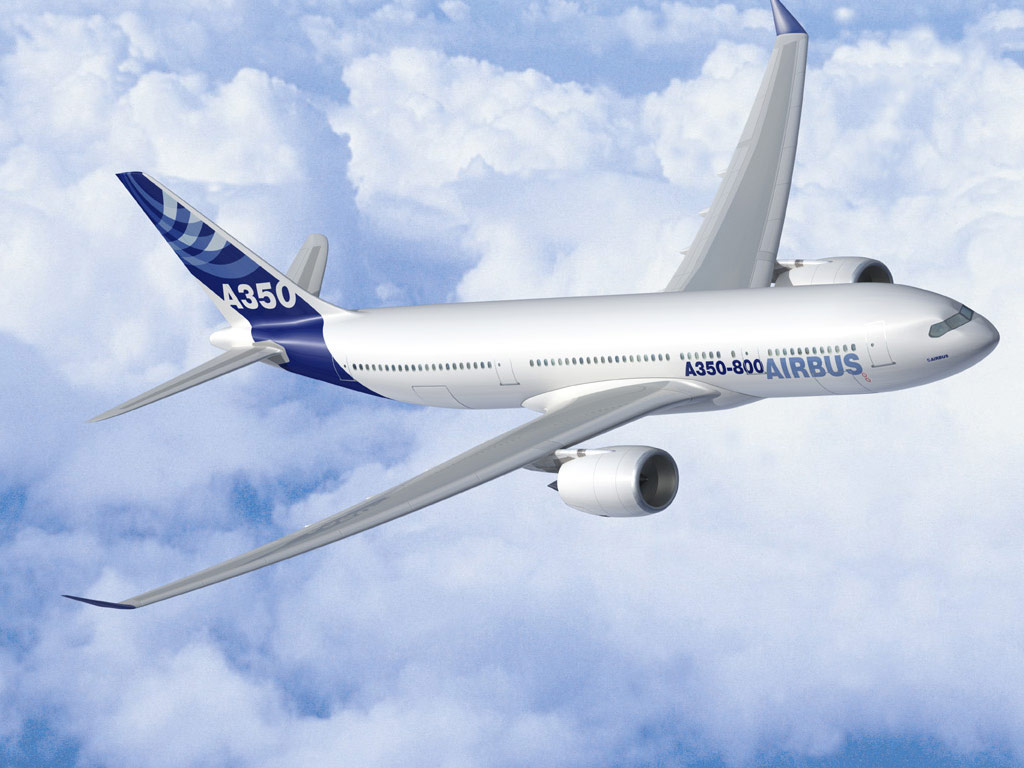
\includegraphics[height=50mm]{Figures/Airbus_A350.jpg}

% Title, author and degree
\vspace{1.0cm}
{\FontLb Prospective studies of highly boosted Higgs pairs decaying to four b quarks} \\ % <<<<< EDIT TITLE
%\vspace{0.2cm}
%{\FontMn Boosted jets resolving power of highly granular hadronic calorimeters} \\
%\vspace{1.9cm}
\vspace{2.6cm}
{\FontMb Ana Luísa Moreira de Carvalho} \\ % <<<<< EDIT NAME
\vspace{2.0cm}
{\FontSn \coverThesis} \\
\vspace{0.3cm}
{\FontLb Engineering Physics } \\ % <<<<< EDIT COURSE
\vspace{1.0cm}
{\FontSn %
\begin{tabular}{ll}
 \coverSupervisors: & José Ricardo Morais Silva Gonçalo \\ % <<<<< EDIT NAME
                    & Pedro Morais Salgueiro Teixeira de Abreu   % <<<<< EDIT NAME
\end{tabular} } \\
\vspace{1.0cm}
{\FontMb \coverExaminationCommittee} \\
\vspace{0.3cm}
{\FontSn %
\begin{tabular}{c}
\coverChairperson:     Jorge Manuel Rodrigues Crispim Romão          \\ % <<<<< EDIT NAME
\coverSupervisor:      José Ricardo Morais Silva Gonçalo \\ % <<<<< EDIT NAME
\coverMemberCommittee: Patrícia Conde Muíño \\ % <<<<< EDIT NAME
\coverMemberCommittee: Kostas Nikolopoulos \\ % <<<<< EDIT NAME
\end{tabular} } \\
\vspace{1.5cm}
{\FontMb October 2018} \\ % <<<<< EDIT DATE (corresponds to date of oral examination)
%
\end{center}

 % file "Thesis_FrontCover.tex"
\cleardoublepage

% ----------------------------------------------------------------------
% Dedication page (optional)
% ----------------------------------------------------------------------
%%%%%%%%%%%%%%%%%%%%%%%%%%%%%%%%%%%%%%%%%%%%%%%%%%%%%%%%%%%%%%%%%%%%%%%%
%                                                                      %
%     File: Thesis_Dedication.tex                                      %
%     Tex Master: Thesis.tex                                           %
%                                                                      %
%     Author: Andre C. Marta                                           %
%     Last modified :  2 Jul 2015                                      %
%                                                                      %
%%%%%%%%%%%%%%%%%%%%%%%%%%%%%%%%%%%%%%%%%%%%%%%%%%%%%%%%%%%%%%%%%%%%%%%%

\null\vskip5cm%
\begin{flushright}
     Dedicated to someone special...
\end{flushright}
\vfill\newpage

 % file "Thesis_Dedication.tex"
\clearpage

% ----------------------------------------------------------------------
%  Acknowledgments (optional)
% ----------------------------------------------------------------------
%%%%%%%%%%%%%%%%%%%%%%%%%%%%%%%%%%%%%%%%%%%%%%%%%%%%%%%%%%%%%%%%%%%%%%%%
%                                                                      %
%     File: Thesis_Acknowledgments.tex                                 %
%     Tex Master: Thesis.tex                                           %
%                                                                      %
%     Author: Andre C. Marta                                           %
%     Last modified :  2 Jul 2015                                      %
%                                                                      %
%%%%%%%%%%%%%%%%%%%%%%%%%%%%%%%%%%%%%%%%%%%%%%%%%%%%%%%%%%%%%%%%%%%%%%%%

\section*{\acknowledgments}

% Add entry in the table of contents as section
\addcontentsline{toc}{section}{\acknowledgments}

%A few words about the university, financial support, research advisor, dissertation readers, faculty or other professors, lab mates, other friends and family...

I would like to express my sincere thanks to my supervisor Ricardo Gon\c calo for his support, invaluable scientific advise and inspirational enthusiasm, without which this work would not have been concluded. To my co-supervisor, Pedro Abreu, I thank for his thorough reading of this thesis and for taking the time to engage in interesting physics discussions. 

I acknowledge the funding of this research by Funda\c c\~ao para a Ci\^encia e Tecnologia - FCT, through CERN/FIS-PAR/0008/2017 grant.

I am very thankful to Patricia Conde and Rute Pedro for fruitful discussions and very helpful advise. To my master colleagues in the LIP ATLAS group, Aidan Kelly, Ant\'onio Costa and Ricardo Barru\'e, I thank for the companionship and motivation throughout this journey. 

I am thankful to Duarte Azevedo, Pedro Ferreira and Rui Santos for being our on-call theoreticians, always available to help.   

I would like to thank all my colleagues in the LIP ATLAS group for making me feel very welcome. I extend my gratitude to everybody at LIP for making it a fantastic place to work. I would also like to acknowledge the LIP IT and secretariat for the technical support.

To the people at CERN, namely Clement Helsens and Michele Selvaggi, I thank for the numerous occasions in which they helped me regarding the FCC software and sample generation. I would also like to acknowledge the CERN IT for the very efficient service. 

I would like to thank my boyfriend, Jo\~ao Augusto, for his never ending patience and unconditional support. To my friends of Chafarrica I express my most sincere thanks for always being a great support, source of joy and laughter. 

To my sister I thank for always welcoming me home with a smile, for the numerous time she offered to help and for all the memes that lighten up some of my days.

To my parents, I will never be able to thank enough. I thank them for their love, unconditional support, inspiration, help in times of need, ... . 
 % file "Thesis_Acknowledgements.tex"
\clearpage

% ----------------------------------------------------------------------
%  Abstract (both in English and Portuguese)
% ----------------------------------------------------------------------
%%%%%%%%%%%%%%%%%%%%%%%%%%%%%%%%%%%%%%%%%%%%%%%%%%%%%%%%%%%%%%%%%%%%%%%%
%                                                                      %
%     File: Thesis_Resumo.tex                                          %
%     Tex Master: Thesis.tex                                           %
%                                                                      %
%     Author: Andre C. Marta                                           %
%     Last modified :  2 Jul 2015                                      %
%                                                                      %
%%%%%%%%%%%%%%%%%%%%%%%%%%%%%%%%%%%%%%%%%%%%%%%%%%%%%%%%%%%%%%%%%%%%%%%%

\section*{Resumo}

% Add entry in the table of contents as section
\addcontentsline{toc}{section}{Resumo}

Inserir o resumo em Portugu\^{e}s aqui com o máximo de 250 palavras e acompanhado de 4 a 6 palavras-chave...

\vfill

\textbf{\Large Palavras-chave:} palavra-chave1, palavra-chave2,...

   % file "Thesis_Resumo.tex"
\clearpage

%%%%%%%%%%%%%%%%%%%%%%%%%%%%%%%%%%%%%%%%%%%%%%%%%%%%%%%%%%%%%%%%%%%%%%%%
%                                                                      %
%     File: Thesis_Abstract.tex                                        %
%     Tex Master: Thesis.tex                                           %
%                                                                      %
%     Author: Andre C. Marta                                           %
%     Last modified :  2 Jul 2015                                      %
%                                                                      %
%%%%%%%%%%%%%%%%%%%%%%%%%%%%%%%%%%%%%%%%%%%%%%%%%%%%%%%%%%%%%%%%%%%%%%%%

\section*{Abstract}

% Add entry in the table of contents as section
\addcontentsline{toc}{section}{Abstract}

%The Electroweak Symmetry Breaking mechanism crucially depends on the value of the Higgs boson self couplings. The Higgs trilinear coupling can be probed using Higgs pair production. However, the small cross-section of this process as well as the overwhelming backgrounds make it a very challenging search. In fact, the observation of this process is most likely out of the reach of the Large Hadron Collider (LHC). Therefore, it will rely on future high energy colliders, making it a key benchmark process.
%
%In particular, the hadronic Future Circular Collider (FCC-hh), expected to work at a center of mass energy of $\sqrt{s}=100$ TeV and to deliver a total integrated luminosity of $O(30)~\text{ab}^{-1}$, is being studied by CERN to start collecting data after the High-Luminosity LHC as reached its full discovery potential, by around 2040. 

The production of pairs of Higgs bosons is a key benchmark process for future colliders because it provides crucial insight into the Electroweak Symmetry Breaking mechanism but it is out of the current reach of the Large Hadron Collider.

CERN is currently leading a study that analyzes the feasibility of a $100$ km circular collider located in the Geneva area. The hadronic Future Circular Collider (FCC-hh) is expected to work at a center of mass energy of $\sqrt{s}=100$ TeV and to collected a total integrated luminosity of $O(30)~\text{ab}^{-1}$.

This thesis describes a Monte Carlo study targeting the search for $hh\rightarrow b\overline{b}$ in a boosted kinematic regime, using proton-proton collisions at center of mass energy of $\sqrt{s}=100$ TeV. The focus is on the impact of the granularity of hadronic calorimeter on the significance, $S/\sqrt{B}$, targeting detector optimization studies for future colliders. In addition to traditional kinematic variables, jet substructure observables are also explored.

For the FCC-hh, the achieved significance is $S/\sqrt{B}=...$ for an integrated luminosity of $\mathcal{L}=30~\text{ab}^{-1}$, which is above the $5\sigma$ threshold. When using particle flow jets, the significance changes very little over the range of detector configurations considered. The change is more accentuated when using pure calorimeter jets.

\vfill

\textbf{\Large Keywords:} keyword1, keyword2,...

 % file "Thesis_Abstract.tex"
\cleardoublepage

% ----------------------------------------------------------------------
%  Table of contents, list of tables, list of figures and nomenclature
% ----------------------------------------------------------------------

% Table of contents
%
\tableofcontents
\cleardoublepage 

% List of tables
%
% Add entry in the table of contents as section
\phantomsection
\addcontentsline{toc}{section}{\listtablename}
% Generate list
\listoftables
\clearpage 

% List of figures
%
% Add entry in the table of contents as section
\phantomsection
\addcontentsline{toc}{section}{\listfigurename}
% Generate list
\listoffigures
\clearpage 

% Nomenclature
%
% entries of nomenclature list
%%%%%%%%%%%%%%%%%%%%%%%%%%%%%%%%%%%%%%%%%%%%%%%%%%%%%%%%%%%%%%%%%%%%%%%%
%                                                                      %
%     File: Thesis_Nomenclature.tex                                    %
%     Tex Master: Thesis.tex                                           %
%                                                                      %
%     Author: Andre C. Marta                                           %
%     Last modified : 21 Jan 2011                                      %
%                                                                      %
%%%%%%%%%%%%%%%%%%%%%%%%%%%%%%%%%%%%%%%%%%%%%%%%%%%%%%%%%%%%%%%%%%%%%%%%
%
% The definitions can be placed anywhere in the document body
% and their order is sorted by <symbol> automatically when
% calling makeindex in the makefile
%
% The \glossary command has the following syntax:
%
% \glossary{entry}
%
% The \nomenclature command has the following syntax:
%
% \nomenclature[<prefix>]{<symbol>}{<description>}
%
% where <prefix> is used for fine tuning the sort order,
% <symbol> is the symbol to be described, and <description> is
% the actual description.

% ----------------------------------------------------------------------
% Roman symbols [r]
\nomenclature[ru]{$\bf u$}{Velocity vector.}
\nomenclature[ru]{$u,v,w$}{Velocity Cartesian components.}
\nomenclature[rp]{$p$}{Pressure.}
\nomenclature[rC]{$C_D$}{Coefficient of drag.}
\nomenclature[rC]{$C_L$}{Coefficient of lift.}
\nomenclature[rC]{$C_M$}{Coefficient of moment.}

% ----------------------------------------------------------------------
% Greek symbols [g]
\nomenclature[g]{$\rho$}{Density.}
\nomenclature[g]{$\alpha$}{Angle of attack.}
\nomenclature[g]{$\beta$}{Angle of side-slip.}
\nomenclature[g]{$\mu$}{Molecular viscosity coefficient.}
\nomenclature[g]{$\kappa$}{Thermal conductivity coefficient.}

% ----------------------------------------------------------------------
% Subscripts [s]
\nomenclature[s]{$x,y,z$}{Cartesian components.}
\nomenclature[s]{$i,j,k$}{Computational indexes.}
\nomenclature[s]{$\infty$}{Free-stream condition.}
\nomenclature[s]{ref}{Reference condition.}
\nomenclature[s]{$n$}{Normal component.}

% ----------------------------------------------------------------------
% Supercripts [t]
\nomenclature[t]{T}{Transpose.}
\nomenclature[t]{*}{Adjoint.}

 % file "Thesis_Nomenclature.tex"
%
% Add entry in the table of contents as section
\phantomsection
\addcontentsline{toc}{section}{\nomname}
% Insert glossary/nomenclature section produced by MakeIndex
\printnomenclature
\clearpage

% entries of glossary list
%%%%%%%%%%%%%%%%%%%%%%%%%%%%%%%%%%%%%%%%%%%%%%%%%%%%%%%%%%%%%%%%%%%%%%%%
%                                                                      %
%     File: Thesis_Glossary.tex                                        %
%     Tex Master: Thesis.tex                                           %
%                                                                      %
%     Author: Andre C. Marta                                           %
%     Last modified : 30 Oct 2012                                      %
%                                                                      %
%%%%%%%%%%%%%%%%%%%%%%%%%%%%%%%%%%%%%%%%%%%%%%%%%%%%%%%%%%%%%%%%%%%%%%%%
%
% The definitions can be placed anywhere in the document body
% and their order is sorted by <symbol> automatically when
% calling makeindex in the makefile
%
% The \glossary command has the following syntax:
%
% \glossary{entry}
%
% The \nomenclature command has the following syntax:
%
% \nomenclature[<prefix>]{<symbol>}{<description>}
%
% where <prefix> is used for fine tuning the sort order,
% <symbol> is the symbol to be described, and <description> is
% the actual description.

% ----------------------------------------------------------------------

\glossary{name={\textbf{MDO}},description={Multi-Disciplinar Optimization is an engineering technique that uses optimization methods to solve design problems incorporating two or more disciplines.}}

\glossary{name={\textbf{CFD}},description={Computational Fluid Dynamics is a branch of fluid mechanics that uses numerical methods and algorithms to solve problems that involve fluid flows.}}

\glossary{name={\textbf{CSM}},description={Computational Structural Mechanics is a branch of structure mechanics that uses numerical methods and algorithms to perform the analysis of structures and its components.}}

\glossary{name={oi}}

 % file "Thesis_Glossary.tex"

% Add entry in the table of contents as section
\phantomsection
\addcontentsline{toc}{section}{\glossaryname}
% Insert glossary section produced by MakeIndex
\printglossary
\clearpage

% Set arabic numbering (1,2,...) after preface
%
\setcounter{page}{1}
\pagenumbering{arabic}

% ----------------------------------------------------------------------
%  Chapters
% ----------------------------------------------------------------------

%%%%%%%%%%%%%%%%%%%%%%%%%%%%%%%%%%%%%%%%%%%%%%%%%%%%%%%%%%%%%%%%%%%%%%%%
%                                                                      %
%     File: Thesis_Introduction.tex                                    %
%     Tex Master: Thesis.tex                                           %
%                                                                      %
%     Author: Andre C. Marta                                           %
%     Last modified :  2 Jul 2015                                      %
%                                                                      %
%%%%%%%%%%%%%%%%%%%%%%%%%%%%%%%%%%%%%%%%%%%%%%%%%%%%%%%%%%%%%%%%%%%%%%%%

\chapter{Introduction}
\label{chapter:introduction}

It is the ultimate goal of particle physics to discover and study all of Nature's fundamental particles and to understand their interactions. Through a joint endeavor of theorists and experimentalists, models that describe particle's dynamics and properties can be precisely probed at collider experiments such as the Large Hadron Collider (LHC). 

We know today that matter particles interact by means of four fundamental forces: electromagnetic, weak, strong and gravitational, of which the first three are associated with mediator particles. We even know that a very special particle, the Higgs boson, is linked to the mechanism that generates the mass of the mediator particles. It is called the Electroweak Symmetry Breaking (EWSB) mechanism and it involves the spontaneous breaking of a gauge symmetry. Through Yukawa couplings, the Higgs boson is also responsible for the masses of fermions. This knowledge is beautifully summarized in the Standard Model of Particle Physics (SM) that was developed in the 1960's and 1970's, long before many of the particles it predicts were discovered. The extraordinary precision of the predictions it delivers make it a very successful model. The Higgs boson, is the most recent elementary particle to be discovered in 2012 at the LHC, which marks an important point in the history of particle physics: we have now found all the particles predicted by the SM and yet we know that it cannot be the whole story. Mainly because there are experimental evidences of physics that it cannot explain.

From the theoretical point of view, this is enough motivation to construct models that extend the SM but that can still deliver predictions that are compatible with experimental data. From the experimental standpoint, this is an indication that we need to keep increasing the precision of our measurements and probing new kinematic regimes in the hope of finding more discrepancies with the SM or some hint that some new phenomenon is taking place.

A higher precision requires a larger integrated luminosity and a larger center of mass energy opens the door for the exploration of new kinematic regimes. Very recently, work towards the upgrade of the LHC to its High-Luminosity (HL) version has began. It is expected to work for a period of ten years between 2026 and 2036 and it will extend the experimental reach of the LHC. In order to keep extending the physics reach of the LHC and HL-LHC, new colliders with unprecedentedly high center of mass (CM) energies are currently being designed in the hope that they begin to deliver data shortly after the HL-LHC has reached its full discovery potential. One of these projects is the hadronic Future Circular Collider (FCC-hh) that consists of a $100$ km ring located in the Geneva area and it is expected to work at a CM energy of $100$ TeV. The FCC-hh will deliver a peak luminosity of $\mathcal{L}=30\times 10^{34}~\text{cm}^{-2}\text{s}^{-1}$ in its ultimate phase. This will result in $O(30)~\text{ab}^{-1}$ per experiment which corresponds to ten times the expected integrated luminosity by the end of the HL-LHC operation. 

The next milestone for the FCC-hh project is the submission of a Conceptual Design Report by the end of 2018. This document will be used as input for the next meeting of the European Strategy for Particle Physics that will take place in the beginning of 2019. It should present a baseline design for the detector, a first cost estimate and preliminary analysis for physics benchmark processes demonstrating the physics reach of such a machine.

Both in the HL-LHC and in future colliders, one of the most important benchmark processes is the production of pairs of Higgs bosons. Firstly, this process is predicted by the SM but has not yet been measured which is due to its very small cross section and overwhelming backgrounds. Furthermore, it provides unique insight into the EWSB mechanism because it is sensitive to the shape of the Higgs potential and can also be used to probe physics beyond the SM (BSM).

In this work we study Higgs pair production at a CM energy of $\sqrt{s}=100$ TeV using the final state with four b quarks. This final state because benefits from the large branching fraction of the Higgs boson to a pair of b quarks. However, in this channel, the multijet production through Quantum Chromodynamics (QCD) interactions is extremely overwhelming. Nonetheless, it is a well known feature of QCD interactions that the partons (and jets) produced tend to have a low transverse momentum ($p_T$). This indicates that exploring a high $p_T$ region of the phase space could be the key to suppress this background. In this kinematic regime, traditional jet reconstruction techniques, that try to establish a one-to-one correspondence between partons and jets, begin to fail because the decay products of heavy and highly boosted particles become more collimated as the $p_T$ of the mother particles increase. State of the art jet reconstruction techniques make use of jets with a larger radius parameter to reconstruct both decay products (two b quarks) as a single jet that can then be used as a proxy for the original particle (a Higgs boson). In order to recover as much information as possible from these jets, it is important to analyze their intrinsic structure, referred to as substructure. 

Jet substructure techniques explore the existence of localized energy maximums inside the large-$R$ jets (subjets). For example, a jet containing the two b quarks from the decay of a Higgs boson is expected to be more consistent with having two subjets than a jet produced by a QCD process. From the standpoint of detector design for the FCC-hh, as well as for future upgrades of existent detectors, the ability to resolve the substructure of large-$R$ jets is a key requirement for which can be helpful a highly granular hadronic calorimeter (HCAL).

The main goal of this thesis is to use boosted di-Higgs production in the four b quarks final state to study the influence of the granularity of the HCAL in significance of the detection that can be achieved.

%Although challenging, this gives us the chance to explore the boosted kinematic regime and jet substructure observables in order to maximize the rejection of this background. We also evaluate the sensitivity of our analysis to BSM benchmark signal processes. From the detector standpoint, we evaluate how the granularity of the hadronic calorimeter influences the analysis' sensitivity and the power to resolve jet's substructure.

Chapter 2 presents an overview of the SM. It summarizes its particle content and interactions and introduces the mathematical formulation of the EWSB breaking mechanism. The successes and shortcomings of the SM are presented and several BSM models are introduced and their motivations discussed. Finally, a theoretical description of the production of Higgs pairs is provided.

The FCC-hh baseline accelerator and detector were highly based on LHC and its current experiments, namely ATLAS and CMS. In chapter 3, after a brief discussion of the general features of particle accelerators, we introduce the LHC and the ATLAS experiment. A discussion of jet reconstruction is included. We then introduce the FCC-hh accelerator and its current baseline detector design. Some key detector parameters are compared to ATLAS.

In chapter 4 we present the state of the art of searches for Higgs pair production at the LHC and of feasibility studies targeting searches for this process at future colliders (High Luminosity LHC and FCC-hh). We also review previous studies that focus on the impact of the HCAL granularity on the jet mass and jet substructure observables resolution.

In chapter 5 we describe in detail the Monte Carlo samples that were used in this work. In addition, the different detector configurations that were tested are described. Chapter 6 entails the description of the analysis strategy and its optimization. A comprehensive characterization of the signal and backgrounds processes is provided. 

In chapter 7 we present and discuss the main results. We focus on the resolution of the jet mass and of the ratio of N-subjetiness variables, namely, $\tau_{21}$. In addition, we analyze how the significance changes as the granularity of the HCAL is varied. The results obtained using particle flow jets and pure calorimeter jets are compared.

Finally, conclusions are drawn in chapter 8.


 % file "Thesis_Introduction.tex"
\clearpage

%%%%%%%%%%%%%%%%%%%%%%%%%%%%%%%%%%%%%%%%%%%%%%%%%%%%%%%%%%%%%%%%%%%%%%%%
%                                                                      %
%     File: Thesis_Background.tex                                      %
%     Tex Master: Thesis.tex                                           %
%                                                                      %
%     Author: Andre C. Marta                                           %
%     Last modified :  2 Jul 2015                                      %
%                                                                      %
%%%%%%%%%%%%%%%%%%%%%%%%%%%%%%%%%%%%%%%%%%%%%%%%%%%%%%%%%%%%%%%%%%%%%%%%

\chapter{The standard model and beyond}
\label{chapter:SM}

The Standard Model (SM) is the theoretical framework that summarizes our present knowledge of particle physics. In section \ref{section:overview_SM}, we provide an overview of this model, focusing on the Higgs mechanism. In section \ref{section:BSM}, we motivate the need to explore models beyond the SM and introduce some of the most well known beyond the SM (BSM) models. In section \ref{section:Higgs_pair}, we provide a theoretical description of the production of Higgs boson pairs which is the physical process that is under study throughout this work.

%In this chapter we review the theoretical, experimental and phenomenological background that support and motivate this work. We briefly describe the Standard Model, including the Higgs mechanism, as well as introduce and motivate some Beyond the Standard Model models. We describe the process of Higgs pair production as a probe of physics both within and beyond the Standard Model (section \ref{section:theoretical}). We briefly review the Large Hadron Collider, its physics program and future upgrades and present a status of the Higgs pair production searches lead by the ATLAS and CMS experiments (section \ref{section:experimental}). We access the Higgs pair production process discovery potential both at the LHC and at future colliders based on feasibility studies (section \ref{section:pheno}). 

%%%%%%%%%%%%%%%%%%%%%%%%%%%%%%%%%%%%%%%%%%%%%%%%%%%%%%%%%%%%%%%%%%%%%%%%
\section{The Standard Model of Particle Physics}
\label{section:overview_SM}

%IDEAS FOR SECTION
%
%- Historic development +  biggest breakthroughs  \\
%- Theoretical description of SM: Symmetry group, Lagrangian, ...\\
%- Biggest successes + experimental confirmations\\
%
%- Theoretical description of Higgs mechanism: symmetry breaking + mass generation for gauge bosons\\
%- Yukawa couplings as a source of mass for leptons

The Standard Model of particle physics summarizes our present knowledge of fundamental particles and their interactions. It is formulated in the framework of Quantum Field Theory (QFT) and describes the subatomic world in terms of fields whose excitations are the particles we can detect. The particle content of the SM is summarized in figure \ref{fig:sm_particles}. Each particle is represented inside a square. The electric and color charge are shown in the right upper corner and the spin in the right lower corner. The mass of the particles are given in electron-Volt (eV) on top of each square (M standing for Million eV and G standing for Billion eV). There are two types of fundamental particles: matter particles and force carriers. 

Matter particles are the building blocks of all the matter in our world. They come in two groups, leptons and quarks. Quarks make up atomic nuclei; leptons, namely electrons and muons, can orbit atomic nuclei forming atoms. Quarks and leptons are elementary fermions which means they have half-integer spin. There are six flavors of quarks: three of the 'up type' (up, charm and top represented by $u$, $d$ and $t$) with electric charge of $+2/3$ and three of 'down type' (down, strange and bottom represented by $d$, $s$ and $b$) with electric charge of $-1/3$. Similarly, we have three leptons with charge $-1$ (electron, muon and tau represented by $e$, $\mu$ and $\tau$) and three neutral leptons (electron, muon and tau neutrinos represented by $\nu$ with the symbol of the corresponding charged lepton as subscript) that are, within the SM, massless. We can classify quarks and leptons in three generations, each composed of an up type and down type quark or of a charged lepton and the corresponding neutrino.

The force carriers, technically called gauge bosons, are particles associated with the fundamental interactions: strong, electromagnetic, weak and gravitational \footnote{The gauge boson that corresponds to the gravitational force has not yet been found. In addition we still do not have a theory that successfully describes gravitation in the framework of QFT so we will not include the gravitational force or its gauge boson in any of the following discussions. Moreover, the gravitational interaction is not relevant for the energy ranges studied.}. Each interaction can be interpreted as the result of the exchange of the corresponding gauge boson. Gluons ($g$) and the photon ($\gamma$) are the mediators of the strong and electromagnetic interactions, respectively. They are massless, electrically neutral and have spin $1$. The $W^{\pm}$ and $Z$ bosons are the mediators of the weak interaction and have a mass of $80.4$ and $91.2$ GeV, respectively. The $W^+$ and $W^-$ bosons have electric charges of $+1$ and $-1$, respectively and spin $1$. The $Z$ boson is electrically neutral and also has spin $1$. The gauge bosons can also be referred to as vector bosons because they have spin equal to one.

In addition to matter particles and gauge bosons, the theoretical formulation of the SM rests on the existence of the Higgs boson that is an electrically neutral and spin $0$ particle. It has a mass of $125$ GeV and it interacts with every particle that has mass.

%The fermions, gauge bosons and Higgs boson properties, namely, electric charge, spin and mass are summarized in Table \ref{table:SM}.

\begin{figure}[]
	\centering
	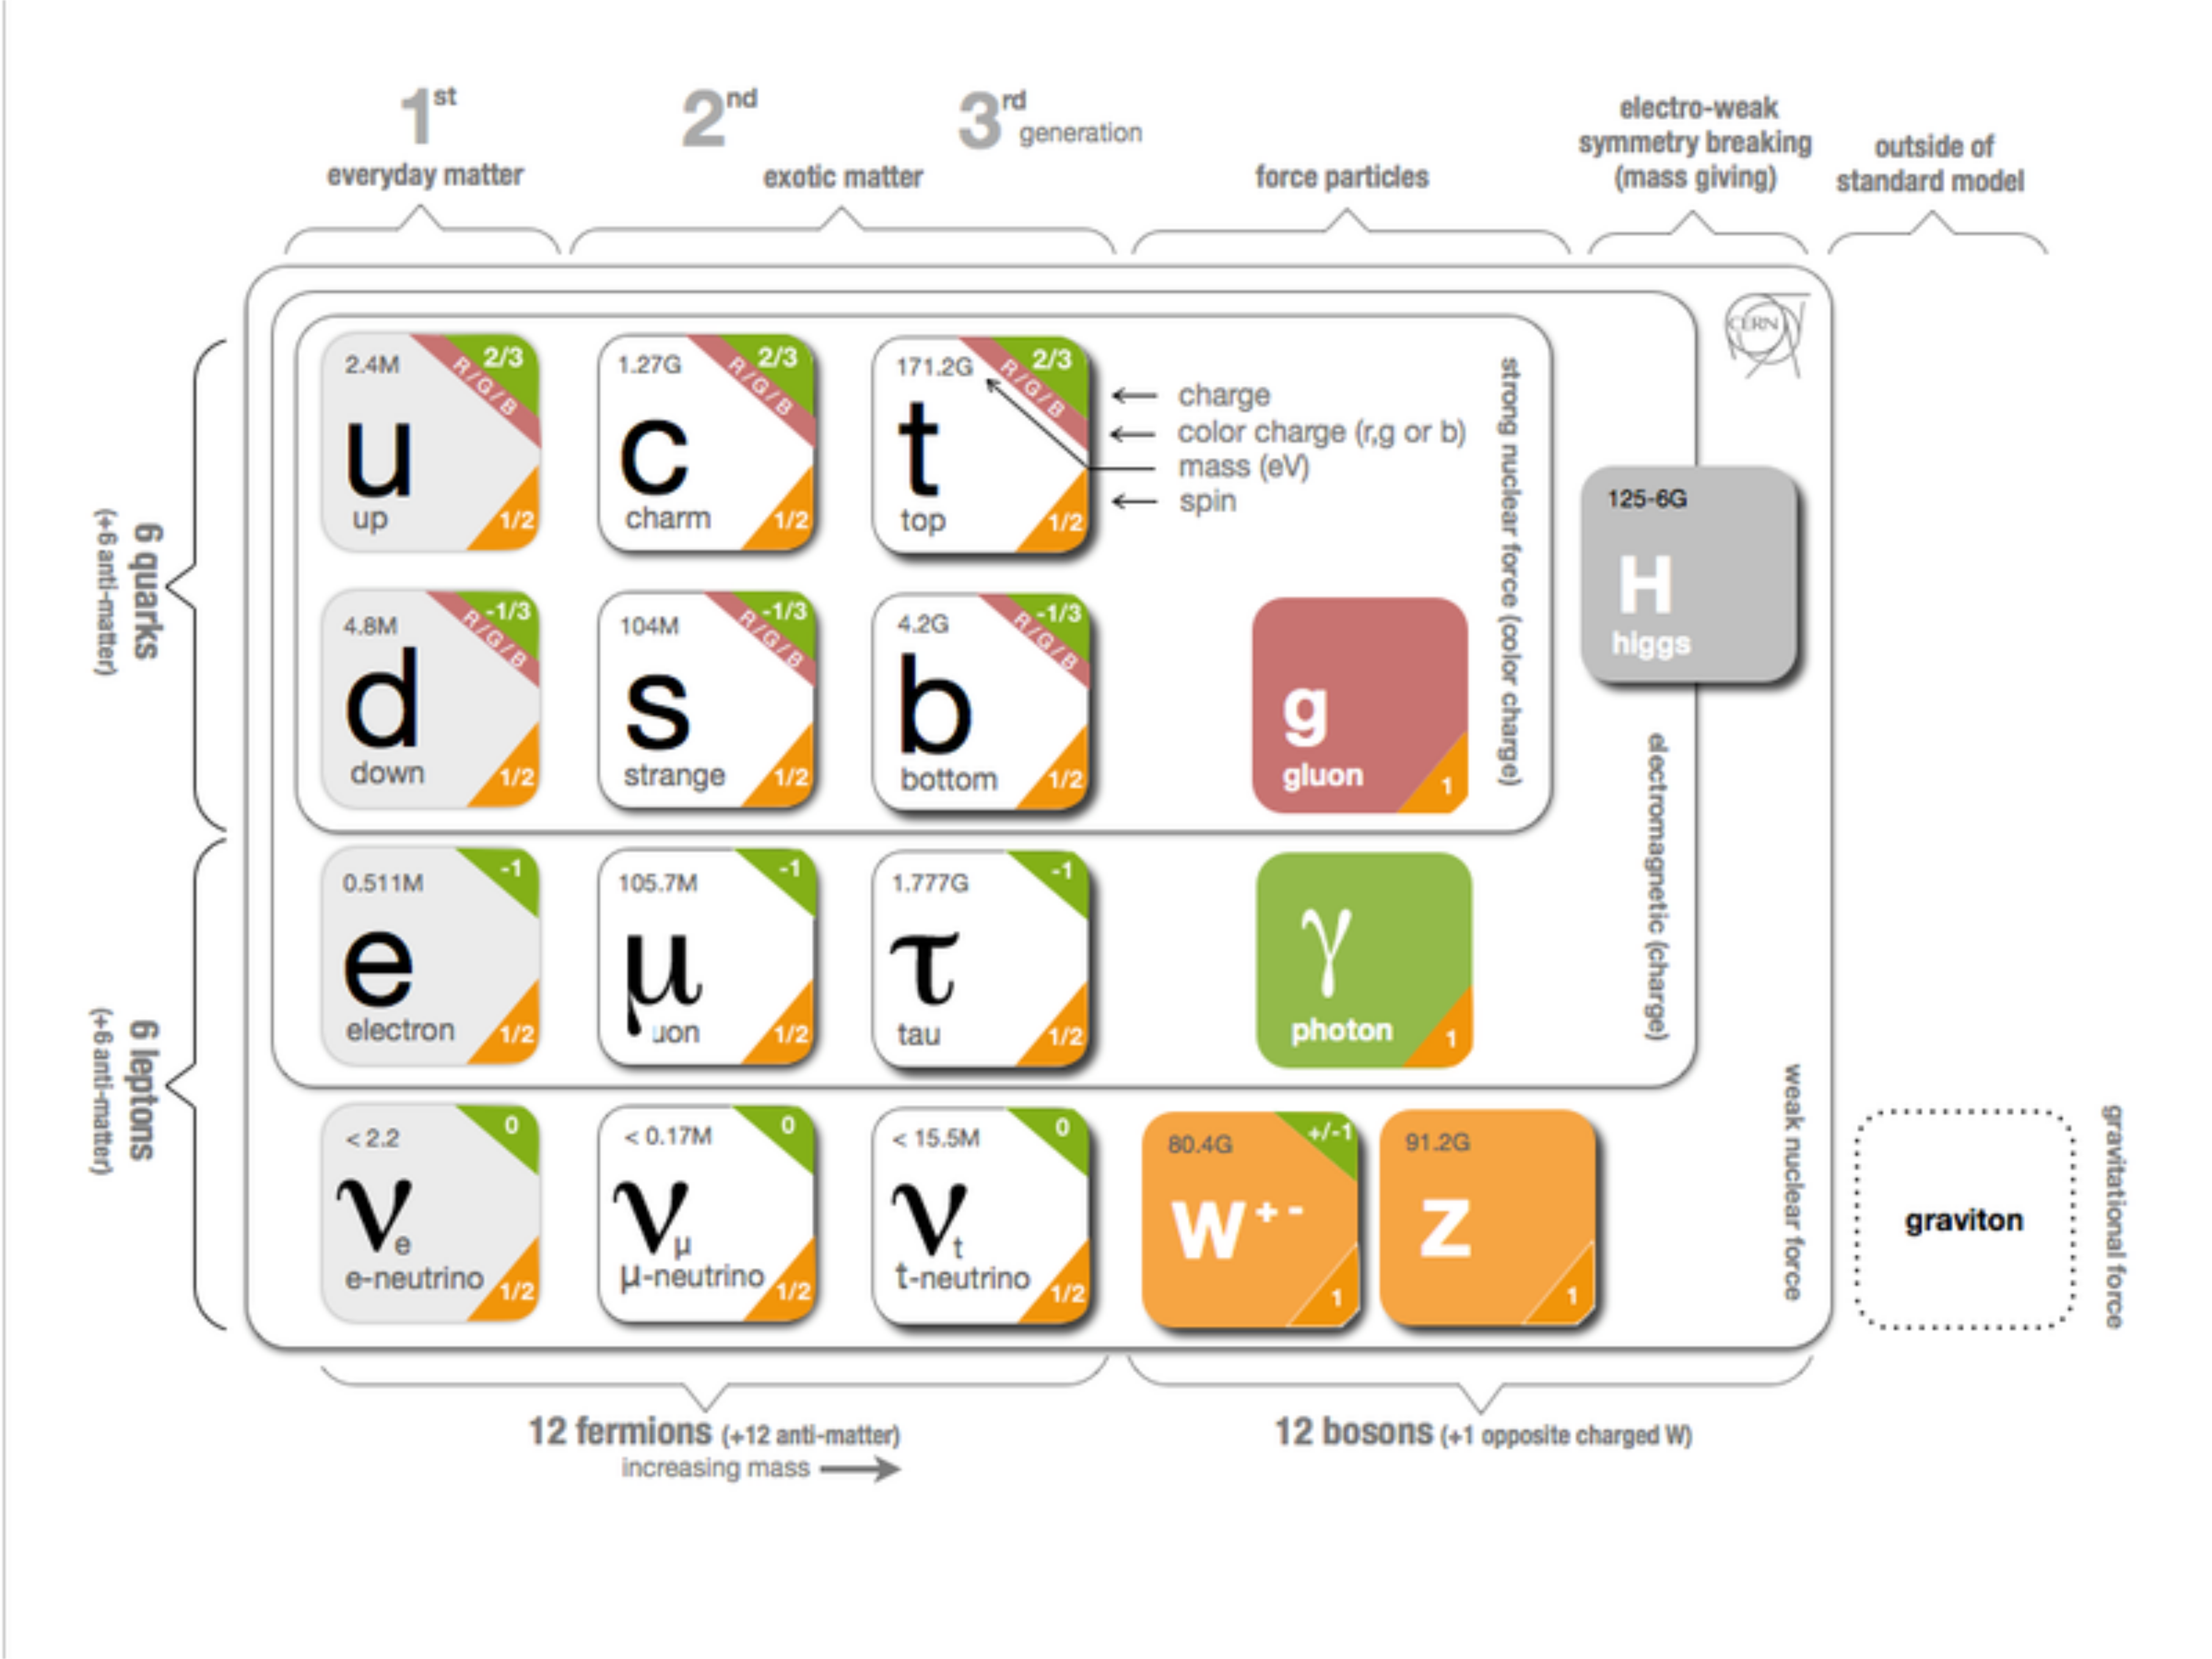
\includegraphics[trim={.5cm 1.5cm 0.5cm 0},clip,width=.8\textwidth]{./Figures/SM_CERN1.png}
	%\caption{Pictorial representation of the SM particles and their interactions. QFD stands for Quantum Flavor Dynamics and BEH stands for Brout-Englert-Higgs. Image from \cite{SMdiv}.}
	\caption{Schematic representation of the Standard Model of elementary particles. Particle are represented inside squares. The electric and color charge are shown in the right upper corner of each square. The spin is shown in the right lower corner. The mass of the particles is also shown, in electron Volt.}
	\label{fig:sm_particles}
\end{figure}

%\begin{table}
%	\centering
%	\begin{tabular}{lllll}
%		\toprule 
%		Type& Particles & Electric charge & Spin & Mass \\
%		\midrule
%		\multirow{2}{*}{Quarks} & $u$, $c$, $t$ & $2/3$ & \multirow{4}{*}{$1/2$}  & $0.0022,1.27,173.21$ GeV\\
%		  & $d$, $s$, $b$ & $-1/3$ &  & $0.0047,0.096,4.18$ GeV\\
%		\multirow{2}{*}{Leptons} & $e$, $\mu$, $\tau$ & $-1$ &  &  $0.51,105.66,1776.86$ MeV\\
%		& $\nu_e$, $\nu_{\mu}$, $\nu_{\tau}$ & $0$ &  & $<2$ eV \\
%		\midrule \midrule
%		\multirow{4}{*}{Gauge bosons} & $g$ &$0$ &\multirow{4}{*}{$1$} & $0$\\
%		 & $\gamma$ & $0$ &  &  $< 10^{-18}$ eV\\
%		 & $W^{\pm}$ & $\pm 1$& & $80.385$ GeV \\
%		& $Z$ & $0$& & $91.1876$ GeV\\
%		\midrule \midrule
%		Higgs boson & $H$ & $0$ & $0$ & $125.09$ GeV\\
%		\bottomrule
%	\end{tabular}
%	\caption{Summary of the particle content of the SM.}
%	\label{table:SM}
%\end{table}

Historically, an empirically successful quantum theory of electromagnetism, Quantum Electrodynamics (QED), was developed in the late 1940's. In the early 1950's there were high hopes that quantum theories could also be formulated for the weak and strong interactions. This is the context in which Yang-Mills theories emerged. They extend the concept of gauge theory from abelian groups, that led to the development of QED, to non-abelian gauge groups. However, the quanta of the fields predicted by these theories must be massless in order to maintain gauge invariance. Therefore, they were set aside until the 1960's when the idea of particles acquiring mass through symmetry breaking in massless theories was put forward by Goldstone \cite{Goldstone}, Nambu and Jona-Lasinio \cite{Nambu-Jona-Lasinio}. In the following paragraphs we discuss in more detail the caveats of Yang-Mills theories and the phenomenon of Spontaneous Symmetry Breaking (SSB) as the basis of the modern Higgs mechanism. We then describe this mechanism in the framework of the SM.   

On the one hand, if one takes a Yang-Mills theory, it becomes clear that it is not possible to include in the Lagrangian a mass term for the gauge bosons because it is not invariant under a gauge transformation. This would not be a problem if we just wanted to describe electromagnetic or strong interactions because the gauge bosons associated with these interactions, the photon and the gluons, are indeed massless. However, for the weak interactions this is not the case. Even before the discovery of the $Z$ and $W^{\pm}$ bosons \cite{Zdiscovery,Wdiscovery} there was experimental evidence of the short range character of the weak interactions which indicated that the corresponding gauge bosons should be massive. 

On the other hand, spontaneous symmetry breaking (SSB) is a phenomenon through which the invariance of a system under a certain symmetry group is destroyed \cite{SSB}. The system may then be invariant under a subgroup of the initial symmetry but the invariance under the original symmetry group is no longer present. In particle physics, this happens because the vacuum of the system (lowest energy states) does not share the symmetry of the Lagrangian. The SSB mechanism predicts the existence of scalar massless particles, the Nambu-Goldstone bosons, as a consequence of the Goldstone theorem \cite{Goldstone} (the number depends on the number of generators of the original and final symmetry groups). Though, when considering this mechanism we get once again massless particles which does not seem to be a step in the right direction if we wish to describe weak interactions. 

However, the real breakthrough occurs when we combine a theory with local gauge invariance with the mechanism of SSB. In this case the Nambu-Goldstone bosons do not appear and it is possible to give mass to the gauge bosons. This is the Higgs mechanism, proposed independently by P.W. Higgs \cite{Higgs}, F. Englert and R. Brout \cite{EnglertBrout} and by G. Guralnik, C. R. Hagen and T. Kibble \cite{Guralnik} in 1964. 

The SM is a non-abelian gauge theory with spontaneous symmetry breaking. It is locally invariant under the following symmetry group:

\begin{equation}
SU_{color}(3)\times SU_L(2)\times U_Y(1), 
\end{equation} 
where the $SU_{color}(3)$ group describes the strong interactions (QCD) and the $SU_L(2)\times U_Y(1)$ group describes the electroweak interactions. Here, $L$ stands for left and $Y$ stands for hypercharge. In the SM the Higgs mechanism, which we now describe, is realized in the $SU_L(2)\times U_Y(1)$ group. The Lagrangian corresponding to the Higgs and gauge sectors of this theory is given by:

\begin{equation}
\mathcal{L}=(D_{\mu}\phi)^{\dagger}(D^{\mu}\phi)-V(\phi^{\dagger} \phi)-\frac{1}{4} W_{\mu \nu}^a W^{a \mu \nu}-\frac{1}{4} B_{\mu \nu} B^{\mu \nu},
\label{eq:Lagragian}
\end{equation}
where the Higgs potential, $V(\phi^{\dagger} \phi)$, is given by:
\begin{equation}
V(\phi^{\dagger} \phi) = \mu^2 \phi^{\dagger} \phi + \lambda (\phi^{\dagger} \phi)^2.
\label{eq:higgsV}
\end{equation}
%and $W_{\mu \nu}^a~(a=1,2,3)$ and $B_{\mu \nu}$ are field strength tensors associated with the gauge fields of $SU_L(2)$ and $U_Y(1)$, $W_{\mu}^a$ and $B_{\mu}$, respectively. The covariant derivative, $D_{\mu}$, is given by
%\begin{equation}
%	D_{\mu}\equiv \partial_{\mu} + igW_{\mu}^a\frac{\tau^a}{2}+ig'B_{\mu}\frac{\mathbb{1}}{2},
%\end{equation}
%where $\tau^a$ are the Pauli matrices and $g$, $g'$ are the coupling constants of $SU_L(2)$ and $U_Y(1)$, respectively. 
$W^a_{\mu\nu}$ and $B_{\mu\nu}$ are the field tensors, defined as a function of the gauge fields of $SU_L(2)$ and $U_Y(1)$, $W^a_{\mu}~(a=1,2,3)$ and $B_{\mu}$,  respectively:

\begin{align}
	W^a_{\mu\nu}&=\partial_{\mu}W^a_{\nu}-\partial_{\nu}W^a_{\mu}-g\epsilon^{abc}W^b_{\mu}W^c_{\nu} \\
	B_{\mu\nu}&=\partial_{\mu}B_{\nu}-\partial_{\nu}B_{\mu}
\end{align}
where $g$ is the coupling constant associated with the $SU_L(2)$ group and $\epsilon^{abc}$ is the completely anti-symmetric tensor in 3 dimensions. The covariant derivative, $D_{\mu}$, is introduced to preserve local gauge invariance and is given by:

\begin{equation}
	D_{\mu}\phi = \left(\partial_{\mu} + igW^a_{\mu}T^a + i\frac{g'}{2}B_{\mu}\right)\phi.
	\label{eq:covariant_derivative}
\end{equation}
$T^a=\frac{\tau^a}{2}$ (where $\tau^a$ are the Pauli matrices) are the $SU_L(2)$ group generators in the fundamental representation and $g'$ is the coupling constant associated with the $U_Y(1)$ group.

Due to the requirement of Lorentz invariance, only the scalar field, $\phi$, can have a vacuum expectation value (VEV), $v$, different from zero \footnote{The other fields that appear in Eq. \ref{eq:Lagragian} are vector fields. If they were to acquire a VEV different from zero that would break Lorentz invariance.}. The values of $v$ are determined by the minima of the potential:
\begin{equation}
v=0 \qquad \text{or} \qquad v=\sqrt{\frac{-\mu^2}{2\lambda}}.
\end{equation}
For the equation on the right (for which we get $v\neq 0$) we only obtain a real value for $v$ (which is a requirement for the VEV of a theory) if $\mu^2<0$. Therefore we conclude that the equation on the right corresponds to $\mu^2\leq0$ while the equation on the left corresponds to $\mu^2\geq0$. In both cases $\lambda$ has to be larger than zero to guarantee that the energy is bounded from below\footnote{In a purely mathematical formulation this means that the function that represents the Higgs potential is concave upwards.} because in Eq. \ref{eq:higgsV} $\lambda$ is the coefficient of the term with the highest power in $\phi$ and therefore determines the concavity of the potential. 

The shapes of the Higgs potential for $\mu^2>0$ and $\mu^2<0$ are shown in Figures \ref{fig:higgsV}(a) and \ref{fig:higgsV}(b), respectively. For $\mu^2>0$ we have a single minimum located at $\langle\phi\rangle=0$. For $\mu^2<0$ the potential has the shape of a 'Mexican hat'. There is an infinite number of minima located in a circumference centered at zero. In this case the minima occur for $\langle\phi\rangle,\langle\phi^{\dagger}\rangle\neq 0$. Therefore the field acquires a VEV different than zero and this is what leads to the SSB.

%\begin{figure}
%	\centering
%	\begin{subfigure}{.5\textwidth}
%		\centering
%		\includegraphics[trim={0cm 1cm 0cm 2.5cm},clip,width=\linewidth]{/home/user/Desktop/5ano1sem/Tese/ProjetoMEFT/higgsV_NSB.pdf}
%		\caption{$\mu^2>0$}
%	\end{subfigure}%
%	\begin{subfigure}{.5\textwidth}
%		\centering
%		\includegraphics[trim={0cm 1cm 0cm 2.5cm},clip,width=\linewidth]{/home/user/Desktop/5ano1sem/Tese/ProjetoMEFT/higgsV_SB.pdf}
%		\caption{$\mu^2<0$}
%	\end{subfigure}
%	\caption{Shape of the Higgs potential. Spontaneous symmetry breaking happens when the potential has the shape shown on the right.}
%	\label{fig:higgsV}
%\end{figure}

\begin{figure}
	\centering
	\begin{minipage}{.5\textwidth}
		\centering
		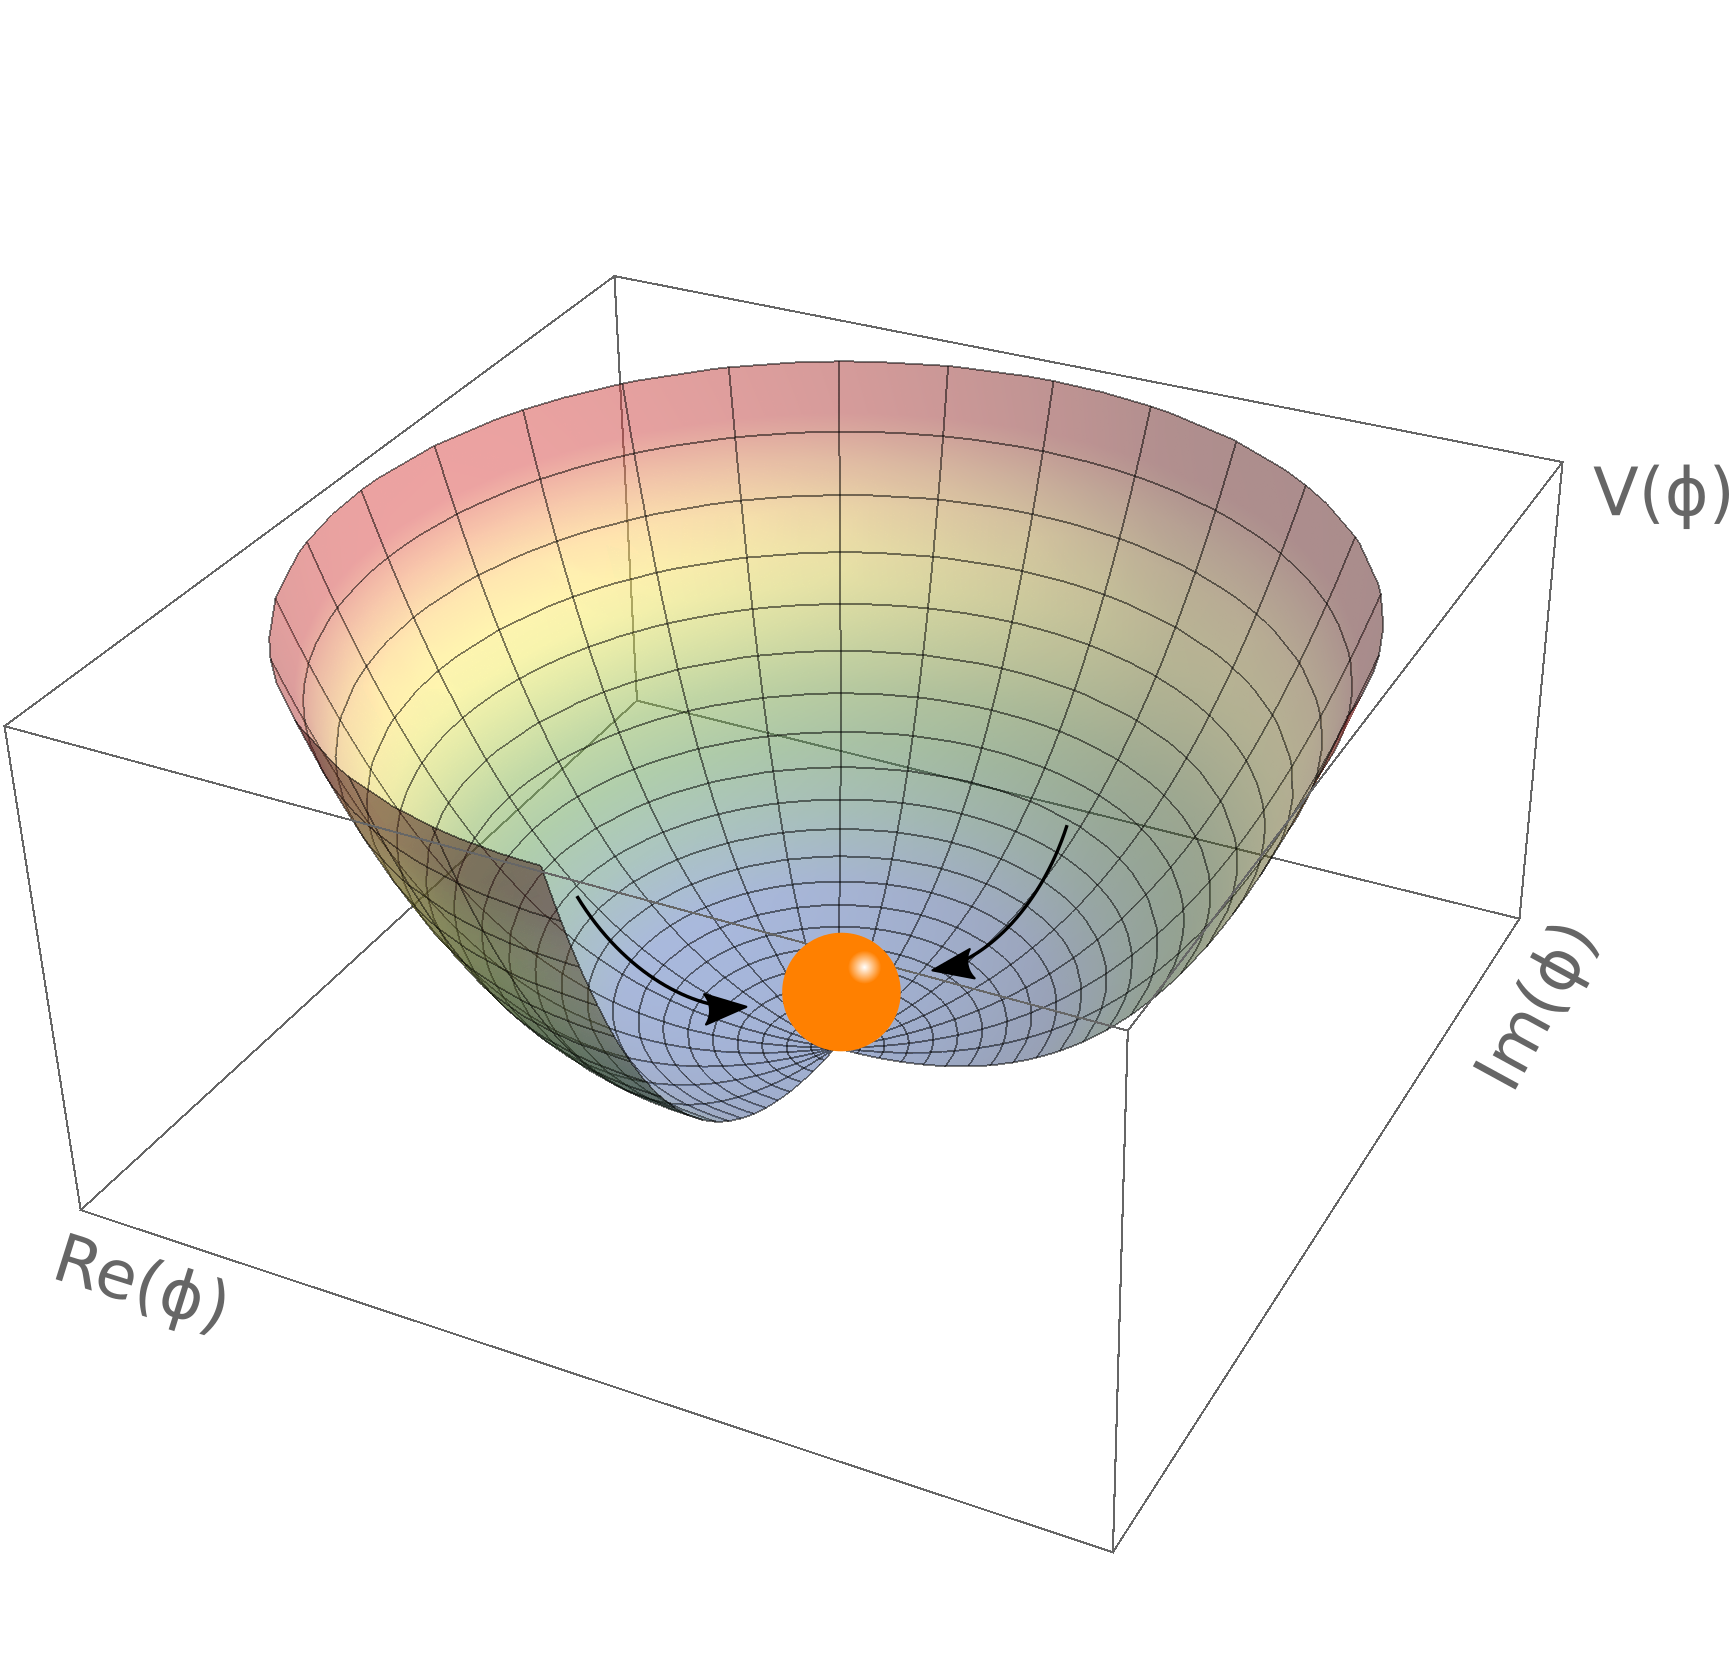
\includegraphics[trim={0cm 1cm 0cm 2cm},clip,width=\linewidth]{./Figures/HiggsV_noEWSB.png}
	\end{minipage}%
	\begin{minipage}{.5\textwidth}
		\centering
		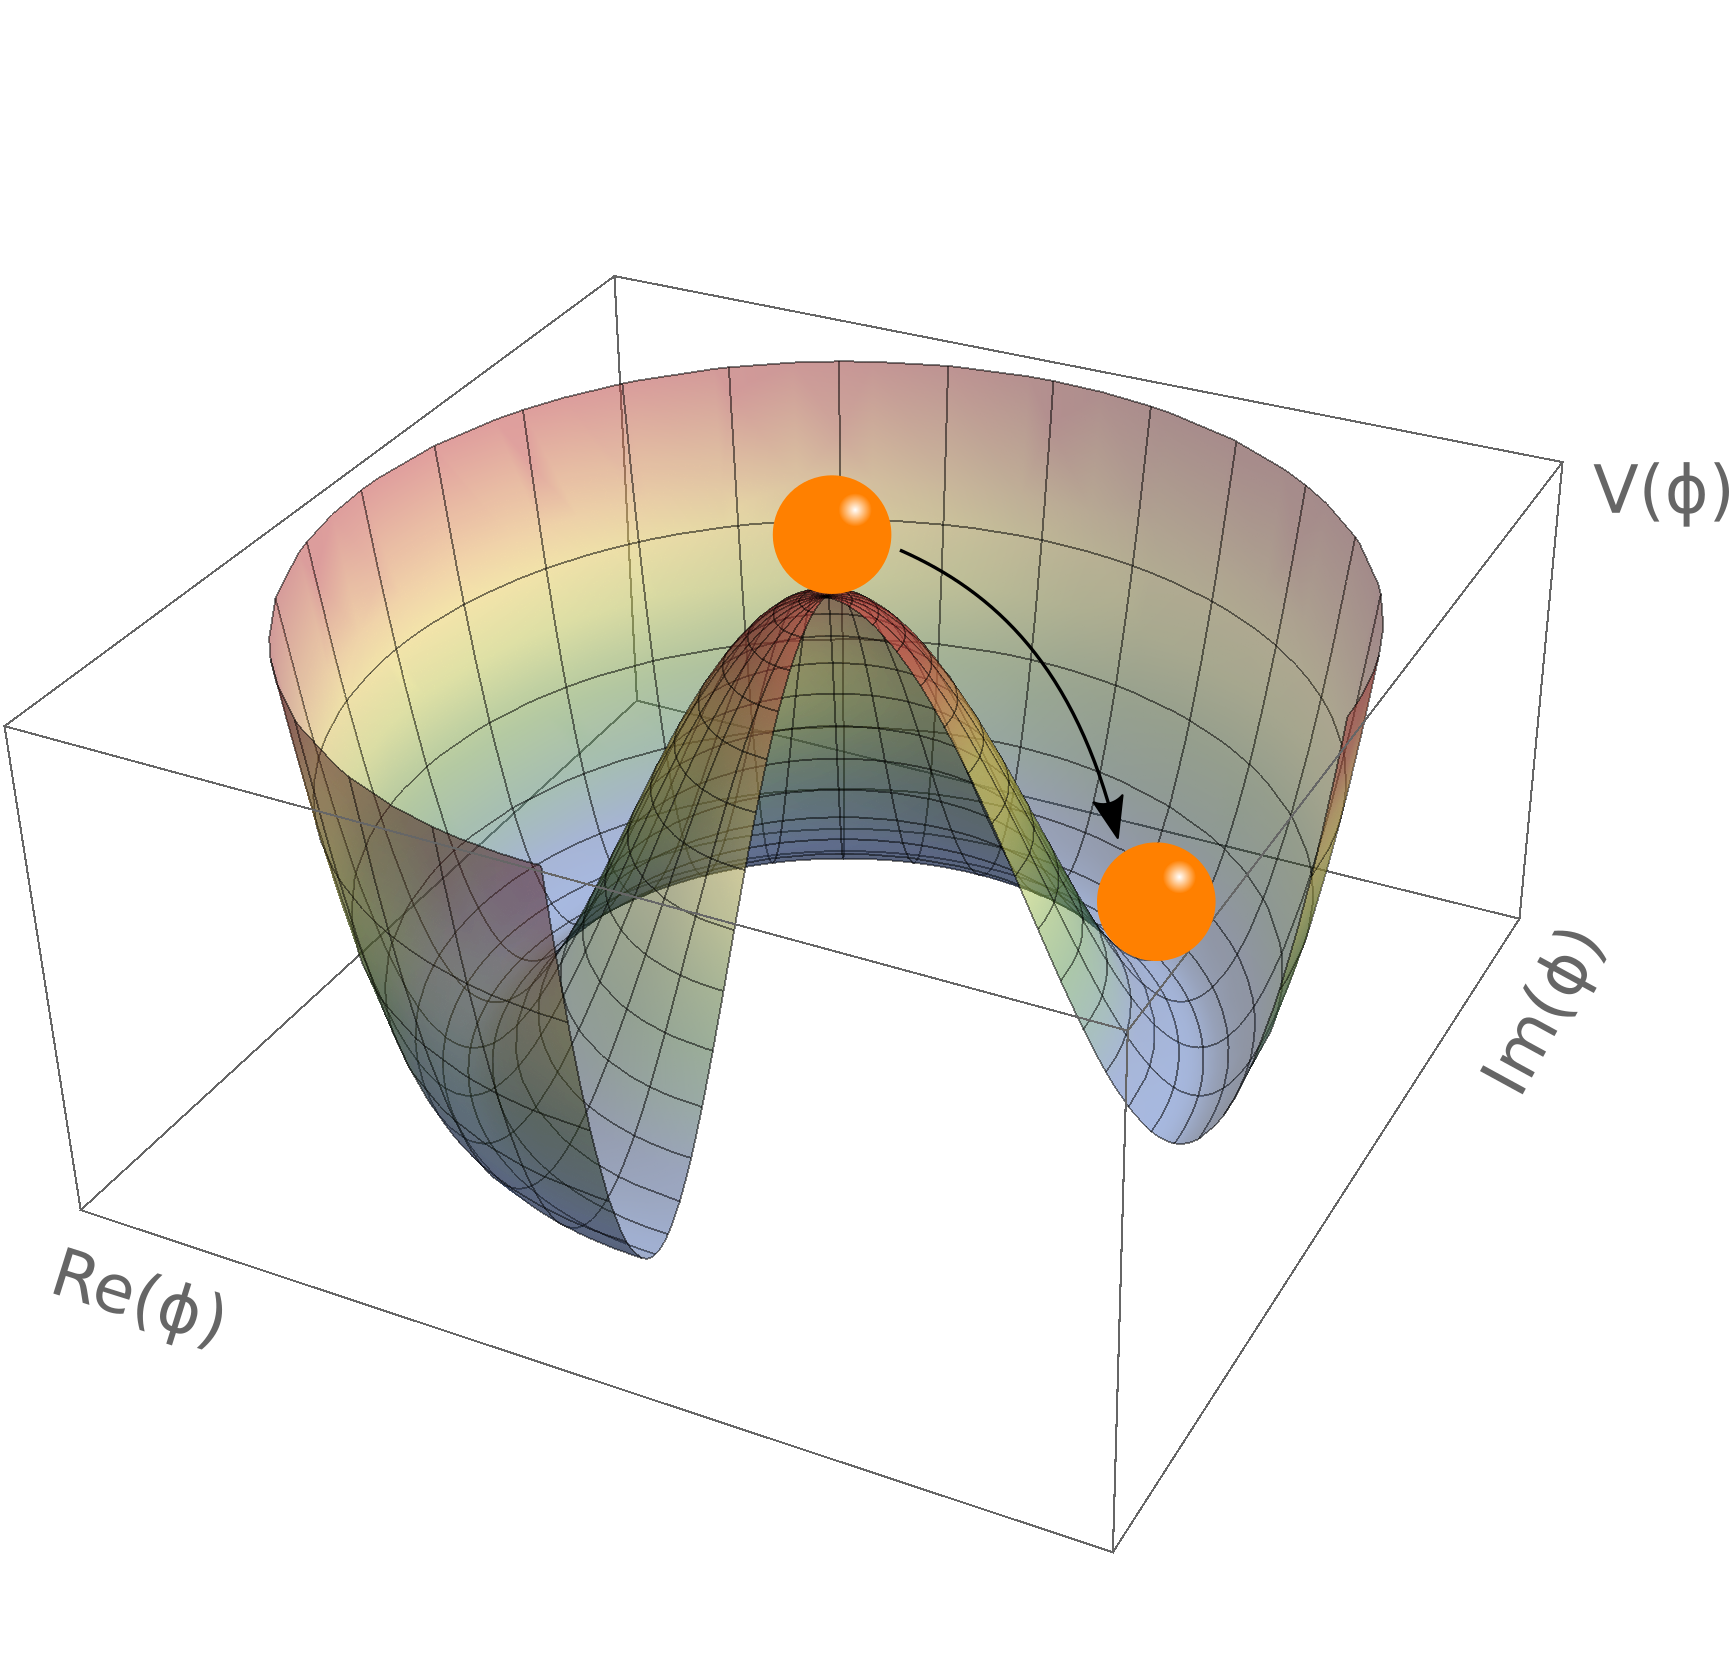
\includegraphics[trim={0cm 1cm 0cm 2cm},clip,width=\linewidth]{./Figures/HiggsV_EWSB.png}
	\end{minipage}
	
	\begin{minipage}[t]{0.5\textwidth}
		\caption*{(a)}
		%\label{fig1}
	\end{minipage}%%%
	\hfill
	\begin{minipage}[t]{0.5\textwidth}
		\caption*{(b)}
		%\label{fig2}
	\end{minipage}
	\caption{Postulated shape of the Higgs potential for $\mu^2>0$ (a) and $\mu^2<0$ (b).}
	\label{fig:higgsV}
\end{figure}

We can now write the scalar field in terms of its minimum value, $v$, and of oscillations around that minimum, $h$ (which corresponds to the Higgs field):
\begin{equation}
\phi = \begin{bmatrix}
0 \\
v+\frac{h}{\sqrt{2}} \\
\end{bmatrix} \qquad (\textit{unitary gauge}).
\label{eq:higgs_field}
\end{equation}
If we expand the first term of the Lagrangian shown in Eq. \ref{eq:Lagragian} using Eq. \ref{eq:covariant_derivative} and Eq. \ref{eq:higgs_field} and taking into consideration that $W^a_{\mu}T^a$ represents a sum over all values of $a$ we get

\begin{align}
	\mathcal{L} = \frac{1}{4}\left(v^2+\frac{h^2}{2}+\frac{2}{\sqrt{2}}vh\right) \left[g^2\left(W^1_{\mu}W^{1\mu}+W^2_{\mu}W^{2\mu}+W^3_{\mu}W^{3\mu}\right)-2gg'B^{\mu}W^3_{\mu}+g'^2 B_{\mu}B^{\mu}\right] + ...~.
	\label{eq:Lagrangian_transform}
\end{align}
We see that for the $W^1_{\mu}$ and $W^2_{\mu}$ fields we have only terms that are quadratic in these fields. These correspond to mass terms. However, for the $W^3_{\mu}$ and $B_{\mu}$ fields there is a term that mixes the two fields. To obtain the physical states of the theory we need to transform these fields in order to get rid of the mixing term which is not physical. We can start by writing the last three terms of Eq. \ref{eq:Lagrangian_transform} in a matrix form and diagonalize the corresponding matrix:
\begin{equation}
\begin{bmatrix}
g^2 & -gg' \\
-gg' & g'^2 \\
\end{bmatrix}
\begin{bmatrix}
W^3_{\mu} \\
B_{\mu} \\
\end{bmatrix}
\xrightarrow{\text{Diagonalization}}
\begin{bmatrix}
0 & 0 \\
0 & g^2+g'^2 \\
\end{bmatrix}
\begin{bmatrix}
A_{\mu} \\
Z_{\mu} \\
\end{bmatrix}.
\label{eq:gauge_matrix}
\end{equation}
$A_{\mu}$ and $Z_{\mu}$ are the physical fields that are related with $W^3_{\mu}$ and $B_{\mu}$ by means of a rotation matrix:
\begin{equation}
\begin{bmatrix}
A_{\mu} \\
Z_{\mu} \\
\end{bmatrix}=
\begin{bmatrix}
\cos\theta_W & -\sin\theta_W \\
\sin\theta_W & \cos\theta_W \\
\end{bmatrix}
\begin{bmatrix}
W^3_{\mu} \\
B_{\mu} \\
\end{bmatrix}
\end{equation}
where $\theta_W$ is the Weinberg angle.
By inverting this relation we can write $W^3_{\mu}$ and $B_{\mu}$ as a function of $A_{\mu}$ and $Z_{\mu}$. Replacing in Eq. \ref{eq:Lagrangian_transform} and imposing that the $A_{\mu}$ field has zero mass we can determine $\theta_W$: $\tan\theta_W=\frac{g'}{g}$. The Lagrangian of Eq. \ref{eq:Lagrangian_transform} takes then the form
\begin{equation}
	\mathcal{L}=\frac{1}{2}\left(v^2g^2\right)\left(W^1_{\mu}W^{1\mu}+W^2_{\mu}W^{2\mu}\right)+\frac{1}{2}\left(v^2\left[g^2+g'^2\right]\right)Z_{\mu}Z^{\mu}+...~,
\end{equation}
where we show only the mass terms for the gauge bosons. Note that, by construction, there is no mass term for $A_{\mu}$ which allows us to identify this field with the photon. $W^1_{\mu}$ and $W^2_{\mu}$ are related to the $W^{\pm}$ boson and $Z_{\mu}$ corresponds to the $Z$ boson. We have shown that it is the fact that $v\neq0$ that allows for the existence of non-zero mass terms for the $W^{\pm}$ and $Z$ bosons.

If we now expand the second term of the Higgs potential (Eq. \ref{eq:higgsV}) using Eq. \ref{eq:higgs_field} we get, among other terms,
\begin{equation}
\mathcal{L}=-h^3\sqrt{-\mu^2 \lambda} - h^4\lambda+...~.
\label{eq:higgs_couplings}
\end{equation}
These terms encode the Higgs self interactions and represent, respectively, the three and four point interactions. We see that the coupling constants of these interactions depend on the parameters of the Higgs potential, $\mu^2$ and $\lambda$.

In addition to being responsible for giving mass to the gauge bosons, the Higgs field is also responsible for the mass of the fermions. However, the mechanism through which this occurs is fundamentally different. In the case of fermions, the mass terms are placed explicitly in the Lagrangian:

\begin{equation}
	\mathcal{L}_{\text{fermions}}=G_1 \overline{L}\phi R + G_2 \overline{L}\phi_c R + \text{hermitian conjugate}
	\label{eq:fermions_mass}
\end{equation}
where $L$ denotes a left-handed fermion doublet and $R$ denotes a right-handed fermion singlet. Here, left and right refer to helicity states. $G_1$ and $G_2$ are arbitrary coupling constants that can be written in terms of the fermion's mass and the VEV. $\phi$ is given by Eq. \ref{eq:higgs_field} and $\phi_c$ is given by (after the spontaneous symmetry breaking and in the unitary gauge):

\begin{equation}
	\phi_c=\begin{bmatrix}
	v+\frac{h}{\sqrt{2}} \\
	0 \\
	\end{bmatrix}.
\end{equation}

We now take a quick detour to motivate why fermions are represented as chiral states (left and right) of the $SU_L(2)$ symmetry. We base this discussion on Ref. \cite{rute}. In the context of the unification of the electromagnetic and weak forces, formalized by Weinberg, Glashow and Salam in 1961, both interactions are interpreted as manifestations of the electroweak force. Weak charged currents are axial vector currents which means they couple only to left handed fermions while weak neutral currents, as well as QED, couple to both helicity states. This suggested that fermions were better represented as left-handed doublets and right-handed singlets of the $SU_L(2)$ symmetry group. The left handed doublets, $L$, are defined as:
\begin{equation}
L:\begin{pmatrix}
\nu_l \\
l \\
\end{pmatrix}_L,
\begin{pmatrix}
u \\
d' \\
\end{pmatrix}_L
\end{equation}
where $l$ represents an electron, muon or tau, $u$ is any quark of the up type and $d'$ is a quark of the down type. The right-handed states, $R$, are singlets, define as:
\begin{equation}
	R: l_R,u_R,d'_R.
\end{equation} 
In 1956, C. S. Wu \textit{et al.} showed that the weak interaction violates parity conservation \cite{wu}. In 1958, M. Goldhaber \textit{et al.} conducted an experiment that showed that neutrinos are left-handed and anti-neutrinos are right-handed \cite{goldhaber} which is why the SM does not include a right-handed state for neutrinos. 
We can now continue the discussion of the mass generation mechanism for fermions.

The first term in Eq. \ref{eq:fermions_mass} gives mass to down type fermions (electron, muon, tau, down, strange and bottom quarks) and the second to up type fermions (up, charm and top quarks). In addition, these terms give rise to the interaction terms between the Higgs field and the fermions. Take, as an example, $\overline{L}=(\overline{t}, \overline{b})_L$ and $R=b_R$. For the first term of Eq. \ref{eq:fermions_mass} we get:

\begin{equation}
	G_1 \overline{L}\phi R = G_1 ~(\overline{t}, \overline{b})_L \begin{bmatrix}
	0 \\
	v+\frac{h}{\sqrt{2}} \\
	\end{bmatrix} b_R = G_1 v ~\overline{b}_L b_R + \frac{G_1}{\sqrt{2}} \overline{b}_L b_R h.
\end{equation}
The first term is the mass term for b quarks. Therefore we can redefine $G_1 v = m_b$ and obtain:
\begin{equation}
	G_1 \overline{L}\phi R=m_b \overline{b}_L b_R + \frac{m_b}{v\sqrt{2}} \overline{b}_L b_R h.
\end{equation}
The second term gives the interaction between the Higgs boson and the fermions, in this case, the b quarks. The strength of this interaction is directly proportional to the mass of the corresponding fermion.

In the SM formalism, neutrinos as massless particles. However, there is no reason why they cannot acquire mass through a mechanism similar to the one we just described. Nonetheless, the usual argument is that it would be unnatural for the same mechanism to produce the mass of very heavy particles, such as the top quark, and the mass of very light particle, such as the neutrinos. Therefore, BSM models that try to explain the mass generation for neutrinos usually resort to a different mechanism.

%\begin{equation}
%	\mathcal{L}_{leptons}=\sum_f \overline{\Psi}_f \left(i\slashed{D}-M\right)\Psi_f,
%\end{equation}
%where $f$ represents any fermion, $\Psi_f$ is a Dirac spinor $\slashed{D}$ is given by ...  and $M$ is a mass matrix. 

The SM has delivered extremely accurate predictions about the existence and properties of new particles which make it a very successful theory. It predicted the existence of the W and Z bosons \cite{Glashow-Weinberg-Salam}, the gluon, the charm and top quarks and the Higgs boson \cite{Higgs,EnglertBrout,Guralnik}. In addition, the SM prediction for the value of the anomalous magnetic dipole moment of the electron (calculated up to order $\alpha^5$) agrees with the measured value up to the $11^{th}$ decimal place, making it the most precise measurement in science.

%
%A reference can be cited in any of the following ways:
%%
%\begin{itemize}
%  \item Citation mode \#1 - \quad \cite{jameson:adjointns}
%  \item Citation mode \#2 - \quad \citet{jameson:adjointns}
%  \item Citation mode \#3 - \quad \citep{jameson:adjointns}
%  \item Citation mode \#4 - \quad \citet*{jameson:adjointns}
%  \item Citation mode \#5 - \quad \citep*{jameson:adjointns}
%  \item Citation mode \#6 - \quad \citealt{jameson:adjointns}
%  \item Citation mode \#7 - \quad \citealp{jameson:adjointns}
%  \item Citation mode \#8 - \quad \citeauthor{jameson:adjointns}
%  \item Citation mode \#9 - \quad \citeyear{jameson:adjointns}
%  \item Citation mode \#10 - \quad \citeyearpar{jameson:adjointns}
%\end{itemize}
%%
%Several citations can be made simultaneously as \citep{nocedal:opt,marta:ijcfd}. \\
%
%This is often the default bibliography style adopted (numbers following the citation order), according to the options:\\
%{\tt \textbackslash usepackage\{natbib\}} in file {\tt Thesis\_Preamble.tex},\\
%{\tt \textbackslash bibliographystyle\{abbrvnat\}} in file {\tt Thesis.tex}.\\
%
%Notice however that this style can be changed from numerical citation order to authors' last name with the options: \\
%{\tt \textbackslash usepackage[numbers]\{natbib\}} in file {\tt Thesis\_Preamble.tex},\\
%{\tt \textbackslash bibliographystyle\{abbrvunsrtnat\}} in file {\tt Thesis.tex}. \\
%
%Multiple citations are compressed when using the {\tt sort\&compress} option when loading the {\tt natbib} package as {\tt \textbackslash usepackage[numbers,sort\&compress]\{natbib\}} in file {\tt Thesis\_Preamble.tex}, resulting in citations like \citep{marta:ijcfd1,marta:ijcfd2,marta:ijcfd3,marta:ijcfd4}.

\subsection{Higgs pair production}
\label{section:Higgs_pair}

%IDEAS FOR SECTION
%
%- Main production process and Feynman diagrams \\
%- Computation of cross section + dependency with COM energy and triple coupling\\
%- Sensitivity to shape of Higgs potential\\
%- Conclude and motivate why this process should be studied (within and beyond SM)

Within the SM there are still some processes that have not been measured. One of these is the production of pairs of Higgs bosons. The experimental challenges and efforts related to this process are discussed in section \ref{section:previous_searches}. Here we provide a theoretical description of the process.

At the Large Hadron Collider (LHC), the main production process of Higgs pairs is gluon-gluon fusion (ggF). Higgs pairs can also be produced through vector boson ($V$) fusion (VBF), in association with a pair of top quarks ($t\overline{t}h$) or through Higgs strahlung ($Vh$) \footnote{In this process, at LO, a Higgs boson is radiated from a vector boson}. At a center of mass (CM) energy of $\sqrt{s}=13$ TeV, the ggF production process has a cross section approximately seventeen times larger than the next most commom production process which is VBF (approximately $30$ fb \textit{versus} $1.6$ fb \cite{hhxsNLO}). Therefore it is the dominant contribution when we study inclusive production. For this reason we focus the following discussion on this production mode. The leading order Feynman diagrams for Higgs pair production via ggF are shown in figure \ref{fig:higgs_pair}. 

%\footnote{There are no tree level diagrams diagrams that contribute to this process. Therefore, the leading order diagrams are at on loop order.}

%\begin{table}
%	\centering
%	\begin{tabular}{lll}
%		\toprule 
%		& \multicolumn{2}{c}{Cross section [pb]} \\
%		Production mode & $14$ TeV & $100$ TeV  \\
%		\midrule
%		ggF & $50.3$ & $740.0$\\
%		\rowcolor{black!7} VBF & $4.4$ & $82.0$\\
%		$t\overline{t}h$ & $0.6$ & $37.9$ \\
%		\rowcolor{black!7} $Zh$ & $0.9$ & $11.3$\\
%		$Wh$ & $1.6$ & $15.9$ \\
%		\bottomrule
%	\end{tabular}
%	\caption{Cross sections in pb for the different Higgs production processes at $14$ and $100$ TeV.}
%	\label{table:Hprod}
%\end{table}

%The diagrams interfere destructively which is indicated by the minus sign between them.

The diagram on the right has an off-shell (virtual) Higgs boson, $h^*$, that couples to gluons by the usual heavy quark triangle (same mechanism as in single Higgs production). $h^*$  then decays to two on-shell Higgs bosons. This diagram contains the three point interaction between Higgs bosons and therefore it is the one that allows us to probe this coupling. In the diagram on the left, the two Higgs bosons couple to the gluons by a box of heavy quarks and are directly radiated from a quark. The largest contributions for these quantum loops come from heavy quarks, such as the top and bottom, because the coupling constant of the Higgs boson to fermions is directly proportional to the fermions mass (see section \ref{section:overview_SM}).

\begin{figure}[h]
	\centering
	\feynmandiagram[baseline=(current bounding box.center),large, layered layout,horizontal=a to b] {
		% Draw the top and bottom lines
		i1 -- [gluon, edge label'=\(g\)] a-- [anti fermion] b-- [scalar, edge label'=\(h\)] f1,
		i2 -- [gluon, edge label'=\(g\)] c-- [fermion] d-- [scalar, edge label'=\(h\)] f2,
		% Draw the two internal fermion lines
		{ [  same layer	] a -- [fermion] c },
		{ [  same layer] b -- [anti fermion] d},
	};\qquad \--- \qquad
	\feynmandiagram [baseline=(current bounding box.center),large, horizontal=e to f] {
		a -- [gluon, edge label'=\(g\)] b -- [anti fermion] c -- [gluon, edge label'=\(g\)] d,
		b -- [fermion] e -- [fermion] c,
		e -- [scalar, edge label'=\(h^*\)]  f,
		h -- [scalar, edge label'=\(h\)] f -- [scalar, edge label'=\(h\)] i,
		a -- [opacity=0] d,
	}; 
	\caption{Feynman diagrams of Higgs pair production from gluon fusion. Triple vertex diagram (left) and box diagram (right). The minus sign between the diagrams indicates that they interfere destructively.}
	\label{fig:higgs_pair}
\end{figure}


The amplitudes for the box, $\mathcal{M}_{\Box}$, and triangle, $\mathcal{M}_{\triangle}$, diagrams scale as \cite{FCCyellow}:
\begin{equation}
\mathcal{M}_{\Box} \sim \frac{\alpha_s}{4\pi} y_t^2, \qquad \mathcal{M}_{\triangle} \sim \lambda_{hhh} \frac{\alpha_s}{4\pi} y_t^2 \frac{m_h^2}{\hat{s}}\Big(\log \frac{m_t^2}{\hat{s}} + i\pi\Big)^2
\label{eq:hh_M}
\end{equation}
where $\hat{s}$ is the CM energy, $y_t$ is the Yukawa coupling of the top quark, $\alpha_s$ is the eletroweak coupling constant, $\lambda_{hhh}$ is the coupling constant of the Higgs boson three point self-interaction and $m_h, m_t$ are the masses of the Higgs boson and top quark.

At a CM energy of $\sqrt{s}=13$ TeV the cross section for Higgs pair production, as predicted by NLO calculations, is very small, approximatelly $30~\text{fb}$ \cite{hhxsNLO}. It is suppressed due to the destructive interference between the LO diagrams that leads to a $\sim 50\%$ supression of the total cross section \cite{FCCyellow}. Furthermore, the cross section of the triangle diagram is smaller that the one of the box diagram, approximately $4$~fb compared to $30$~fb \footnote{These values are obtained using MadGraph5. They are shown here to give a rough estimate of the difference between the values of the cross sections  of both diagrams.}, and it is strongly suppressed for larger values of the CM energy which can be seen directly from the expression of the amplitude in Eq. \ref{eq:hh_M}. This means that the Higgs trilinear coupling mostly affects the Higgs pair production at threshold. A variable that is sensitive to these effects is the invariant mass of the Higgs pair. The tail of this distribution (high invariant mass of the Higgs pair), however, is mostly determined by the box diagram contribution \cite{FCCyellow}.  

The LO calculation for the cross section of Higgs pair production has been performed, for example, in Ref. \cite{HHxs_LO}. A value of the order of $10$~fb is reported. The NLO calculation is a theoretical challenge: several two-loop diagrams that take into account virtual and real radiation have to be considered. In addition, top quark mass effects can be included in various approximations. This leads to corrections with different signs which suggests that the uncertainty on the cross section due to top quark mass effects are of the order of $\pm 10\%$ at NLO. Therefore, a calculation including the full top mass dependence was of the utmost importance. This result became available recently \cite{HHcalc_top}:
\begin{equation}
\sigma^{\text{NLO}}_{gg\rightarrow hh} = 27.80^{+13.8\%}_{-12.8\%}(\text{scale})\pm 0.3\%(\text{stat.})\pm 0.1\% (\text{int.})~\text{fb}
\end{equation}
where the dependence of the result on the variation of the scales by a factor of two around the central scale, the statistical error coming from the limited number of phase space points evaluated and the error coming from the numerical integration of the amplitude are shown. 

This result shows that the introduction of NLO contributions produces a significantly different result. Therefore the inclusion of such effects is necessary if we wish to obtain an accurate result that can be compared to experimental values. The analytical expressions for the NLO cross section are long and complex so we abstain from reproducing them here. Nonetheless, the LO cross section can be written in a compact form and it allows us to discuss some key features of the process. Therefore, we will present it here, based on Refs. \cite{HHxs_LO,HHxs_LO1}.

The partonic LO cross section for $gg\rightarrow hh$ can be written
\begin{equation}
\hat{\sigma}^{\text{LO}}_{gg\rightarrow h} (\hat{s}) \sim \int_{\hat{t}_-}^{\hat{t}_+}~d\hat{t}~\left(|C_{\bigtriangleup}F_{\bigtriangleup}+C_{\Box}F_{\Box}|^2+|C_{\Box}G_{\Box}|^2\right)
\end{equation}
where $\hat{s}$ and $\hat{t}$ are the Mandelstam variables and, in addition, $\hat{s}$ can be identified with the square of the partonic CM energy of the process. The integration limits, $\hat{t}_{\pm}$, are derived from a momentum parametrization in the CM frame, leading to $\hat{t}_{\pm}=m_h^2-\frac{\hat{s}}{2}(1\mp \beta_h)$, where $\beta_h^2=1-4\frac{m_h^2}{\hat{s}}$ and $m_h$ is the mass of the Higgs boson \cite{HHxs_LO1}. $F_{\bigtriangleup}$, $F_{\Box}$ and $G_{\Box}$ are form factors whose full expressions can be found, for example, in Ref. \cite{HHxs_LO}. $C_{\bigtriangleup}$ and $C_{\Box}$ can be interpreted as generalized couplings and are given by
\begin{equation}
C_{\bigtriangleup}=\lambda_{hhh}\frac{m_Z^2}{\hat{s}-m_h^2}, \qquad C_{\Box}=1,
\end{equation}
where $m_Z$ is the mass of the $Z$ boson.
If we take the limit $m_Q^2 \gg \hat{s}\sim m_h^2$ (where $m_Q$ is the mass of the quarks that contribute to the quantum loops) we can get simple expressions for the remaining form factors:
\begin{equation}
F_{\bigtriangleup}=\frac{2}{3} + \mathcal{O}(\hat{s}/m_Q^2), \qquad F_{\Box}=-\frac{2}{3} + \mathcal{O}(\hat{s}/m_Q^2), \qquad G_{\Box}=\mathcal{O}(\hat{s}/m_Q^2).
\end{equation}
In this limit, the partonic cross section is simply given by 
\begin{equation}
\hat{\sigma}^{\text{LO}}_{gg\rightarrow hh}(\hat{s}) \sim \int_{\hat{t}_-}^{\hat{t}_+}~d\hat{t}~ |\lambda_{hhh}\frac{m_Z^2}{\hat{s}-m_h^2}-1|^2.
\label{eq:xsparton}
\end{equation}

%To get the total cross section we need to integrate over the Parton Distributions Functions (PDFs). Defining the luminosity function as
%\begin{equation}
%\frac{d\mathcal{L}_{ij}}{d\tau} = \sum_{ij}\int_{\tau}^{1}\frac{dx}{x}f_i(x,\mu_F)f_j\left(\frac{\tau}{x},\mu_F\right)
%\end{equation}
%
%the total cross section reads
%\begin{equation}
%\sigma_{gg\rightarrow hh}^{\text{LO}}=\int_{\tau_0}^{1}~d\tau~\frac{d\mathcal{L}_{gg}}{d\tau} ~\hat{\sigma}^{\text{LO}}_{gg\rightarrow hh}(\hat{s}=\tau s),
%\label{eq:fullxs}
%\end{equation}
%where $s$ is the square of the hadronic CM energy, $\tau_0=4m_h^2/s$ and $\mu_F$ is the factorization scale.

There are two important points that are worth discussing. Firstly, the total cross section has terms that are proportional to the Higgs triple couling, $\lambda_{hhh}$, which can be read directly from Eq. \ref{eq:xsparton}. On the one hand, this means that measuring this process gives us access to the value of $\lambda_{hhh}$ and therefore provides valuable insight into the shape of the Higgs potential and ultimately into the EWSB mechanism in the SM. On the other hand, if $\lambda_{hhh}$ has a value that is different from the one predicted by the SM, that will affect the measured value of the cross section and can lead to hints of new physics. 

Secondly, although this is not evident from Eq. \ref{eq:xsparton}, the cross section for di-Higgs production increases with $\hat{s}$. This can be seen in figure \ref{fig:HHxs_s} that shows the variation of the total (integrated) NLO cross section with the CM energy for the six largest production channels. Note that increasing the CM energy from $13$ to $100$ TeV increases the inclusive cross section by approximately two orders of magnitude which is a consequence of the increased phase space that becomes available.

\begin{figure}[]
	\centering
	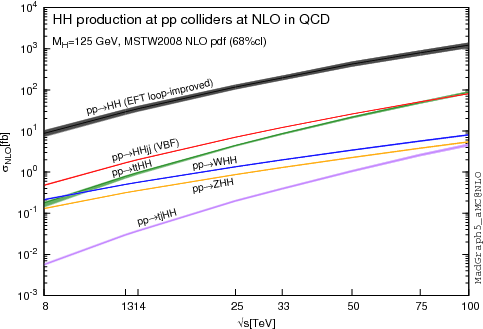
\includegraphics[width=0.6\textwidth]{./Figures/HH-xsec.png}
	\caption{Total cross sections at NLO in QCD for the six largest HH production channels at pp colliders. The thickness of the lines corresponds to the scale and PDF uncertainties added linearly.}
	\label{fig:HHxs_s}
\end{figure}

Therefore, the increase in the cross section of rare processes, such as Higgs pairs production, as the CM energy of collision experiments increases supports the claim that future colliders, with higher CM energies, might be our chance of discovering and precisely studying these processes.

%Nonetheless, if we take the limit $m_Q^2 \gg \hat{s}\sim M_H^2$ we can get simple expressions for the form factors:
%\begin{equation}
%	F_{\bigtriangleup}=\frac{2}{3} + \mathcal{O}(\hat{s}/m_Q^2), \qquad F_{\Box}=-\frac{2}{3} + \mathcal{O}(\hat{s}/m_Q^2), \qquad G_{\Box}=\mathcal{O}(\hat{s}/m_Q^2).
%\end{equation}
%In this limit, the differential cross section is given by 
%\begin{equation}
%	\frac{d\hat{\sigma}}{d\hat{t}} \sim |\lambda_{hhh}\frac{M_Z^2}{\hat{s}-M_H^2}-1|^2.
%\end{equation}
%\begin{figure}[h]
%	\centering
%	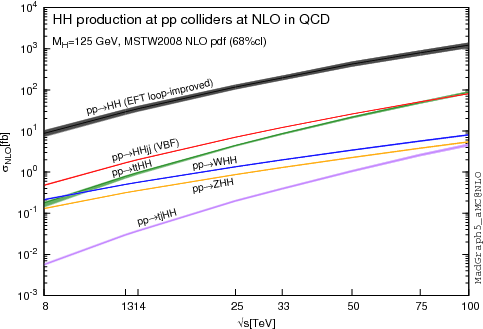
\includegraphics[width=0.7\textwidth]{./Figures/HH-xsec.png}
%	\caption{Total cross sections at the NLO in QCD for the six largest HH production channels at pp colliders. The thickness of the lines corresponds to the scale and PDF uncertainties added linearly.}
%	\label{fig:hh_xsec}
%\end{figure}

%%%%%%%%%%%%%%%%%%%%%%%%%%%%%%%%%%%%%%%%%%%%%%%%%%%%%%%%%%%%%%%%%%%%%%%%
\section{Going beyond}
\label{section:BSM}
%
%IDEAS FOR SECTION
%
%- Why we need to study physics BSM (motivation: theoretical+experimental)\\
%- Brief description of most well known and well studied BSM models that include changes in the Higgs sector, predict heavier Higgs \\
%- How these can be probed using Higgs pair production

Despite the success of the SM, there is evidence that indicates that it cannot be the final theory of particle physics. This led to the development of alternative models that extend the SM but that can still reproduce its successful predictions. These are referred to as Beyond the Standard Model (BSM) models. 

On the one hand, there are several pieces of experimental evidence that the SM cannot explain. These include the nature of dark matter, postulated to explain the experimental observations of the velocity of far away galaxies \cite{DM}, the asymmetry between matter and anti-matter in the present Universe \footnote{Or why do we live a local in an Universe made mostly out of matter?} and the fact that neutrinos oscillate between flavors which implies that they have a non-zero mass. This phenomenon was measured independently by two collaborations, the Super-Kamiokande and the Sudbury Neutrino Observatory (SNO), in 1998 and 2001-2002, respectively, \cite{neutrinosSuperK,neutrinosSNO1,neutrinosSNO2}.

On the other hand, its theoretical formulation also has some weaknesses: it accurately describes particles interactions at the electroweak scale ($\sim 246$~GeV) but it does not include gravity which means it cannot be valid at the Planck scale ($\sim 10^{19}$~GeV) where gravity cannot be overlooked; it has a lot (over $20$) of free parameters whose values have to be tuned to fit experimental observations, and there is a large discrepancy between the mass scales associated with the electroweak and gravitational interactions (this is one of the simplest formulations of what is known as the hierarchy problem).

When faced with these weaknesses, or rather hints of incompleteness, the theoretical community put a great effort into the development of models that add new ingredients to the SM. In the following paragraphs we introduce and briefly describe some of the most well studied (both theoretically and experimentally) BSM models. We follow the discussion presented in Ref. \cite{BSM_motivation} as a starting point.

It is a well known consequence of renormalization in QFT that the coupling constants become dependent on the energy scale at which the theory is probed. As the energy scale increases the $U_Y(1)$ coupling constant gets larger while the $SU_L(2)$ and $SU_{color}(3)$ coupling constants get smaller. If one extrapolates far enough these become nearly equal at an energy scale of approximately $10^{15}$~GeV. Although this matching is far from perfect, it sparked the idea that these three forces could be unified at an energy scale of $10^{15}$~GeV. Grand Unification Theories (GUT) try to combine $SU_{color}(3)\times SU_L(2)\times U_Y(1)$ into a larger symmetry group.

Supersymmetric (SUSY) models introduce a new symmetry that links fermions and bosons. For each boson(fermion) of the SM it introduces a fermionic(bosonic) partner. Apart from spin, the supersymmetric partners would share the same mass and quantum numbers. Since we have not found any supersymmetric particles in the LHC this means that supersymmetry is necessarily a broken symmetry and, if they exist, new particles should have a larger mass (outside of the present reach of the LHC) than their SM partners. SUSY models were introduced because they offer a natural fix for the hierarchy problem. In addition, the Minimal Supersymmetric extension of the SM (MSSM) also leads to a better convergence of the coupling constants as can be seen in figure \ref{fig:SM_MSSM}. From the standpoint of GUT this is extremely appealing.

\begin{figure}
	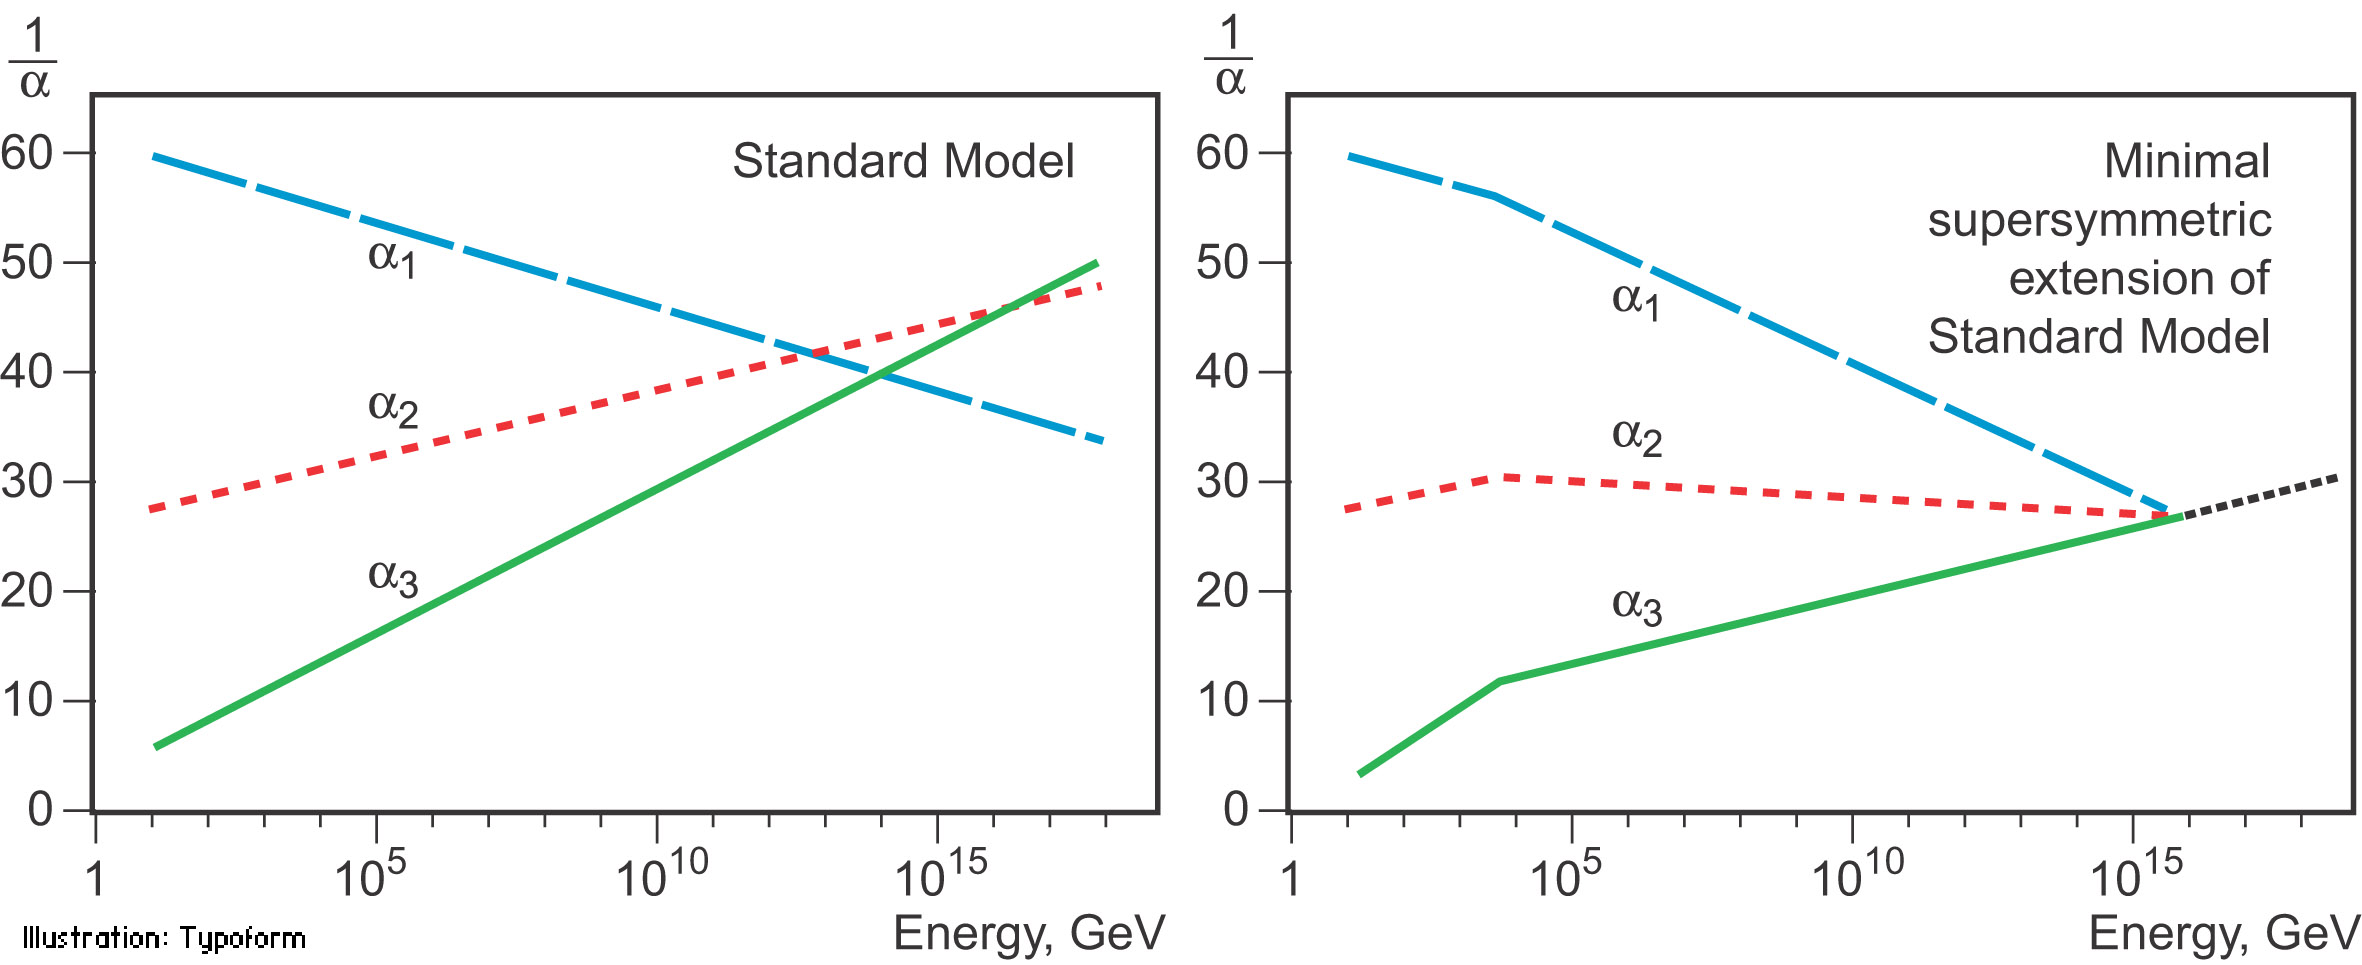
\includegraphics[width=\textwidth]{Figures/SM_MSSM.jpg}
	\caption{Here, $\alpha_1$, $\alpha_2$ and $\alpha_3$ represent the coupling constants of $U_Y(1)$, $SU_L(2)$ and $SU_{color}(3)$, respectively. What is shown is the variation of the inverse of the coupling with the energy: on the left for the SM and on the right for the MSSM. Plots from Ref. \cite{running_coupling}.}
	\label{fig:SM_MSSM}
\end{figure}

An early proposal of a theory that could unify gravity with electromagnetism was given by Theodore Kaluza in 1921. In particular, he showed that these two forces could stem from a single tensor with the introduction of an extra space dimension. In 1926, Oscar Klein offered an explanation for this extra dimension; he proposed that it had a circular topology such that at each point of the four dimensional space-time we would have a circle with a small radius. This theory has more degrees of freedom (because it is formulated in a higher dimensional space-time) and therefore it predicts new particles that are usually known as Kaluza-Klein gravitons (and their excited states). Nonetheless, the Kaluza-Klein model does not provide a satisfactory explanation for the hierarchy problem. Therefore, in 1999, Lisa Randall and Raman Sundrum introduced a new model that does. This model introduces only two new particles: a spin 2 graviton (and its Kaluza-Klein excitations) and a radion, that is a spin 0 neutral particle.

Models with two Higgs doublets (2HDM) are one of the simplest possible extensions of the Higgs sector of the SM. They are appealing because while the fermionic sector is rather complex, having three families, the scalar sector is quite simple, having a single particle, which seems unnatural. This type of structure is realized in various new physics models including SUSY models. In addition, they provide an additional source for CP violation which could help explain the matter-anti-matter asymmetry in the Universe. 

The most general renormalizable 2HDM scalar potential is written as \cite{2HDMpedro}
\begin{align}
	V&=m_{11}^2 |\Phi_1|^2+m_{22}^2 |\Phi_2|^2-(m_{12}^2 \Phi_1^{\dagger}\Phi_2+h.c.)\nonumber \\
	&+\frac{1}{2}\lambda_1|\Phi_1|^4+\frac{1}{2}\lambda_2|\Phi_2|^4+\lambda_3|\Phi_1|^2|\Phi_2|^2+\lambda_4|\Phi_1^{\dagger}\Phi_2|^2 \nonumber \\
	&+\left[\frac{1}{2}\lambda_5\left(\Phi_1^{\dagger}\Phi_2\right)^2+\lambda_6 |\Phi_1|^2\left(\Phi_1^{\dagger}\Phi_2\right)^2+\lambda_7 |\Phi_2|^2\left(\Phi_1^{\dagger}\Phi_2\right)^2+h.c.\right],	
	\label{eq:2HDMpot}
\end{align}  
where $\Phi_1$ and $\Phi_2$ are hypercharge doublets and the coefficients $m_{12}^2$ and $\lambda_{5,6,7}$ can be complex. However, when including the Yukawa interactions, the most general lagrangian leads to tree-level flavor changing neutral currents (FCNC) in the Yukawa sector. These FCNC are very tightly constrained by experimental data and should be avoided. They can be eliminated by imposing a $\mathbb{Z}_2$ symmetry. Although, usually, this symmetry is allowed to be softly broken in order to allow the theory to have a decoupling limit \cite{2HDMdec} where the mass of all the scalars other than the SM-like one can be made very large. In addition to the softly-broken $\mathbb{Z}_2$ symmetry, which leads to $\lambda_{6,7}=0$, we also impose CP conservation which makes all possible complex phases vanish. In this case, we obtain five Higgs bosons that are CP eigenstates. Three of them are neutral, $h$, $H$ and $A$, and the other two are charged, $H^{\pm}$. $h$ and $H$ are CP-even states while $A$ is CP-odd. $h$ is usually taken to be the SM Higgs boson and its mass is set to $125$ GeV.

There are several types of 2HDM classified according to their fermion-scalar interactions. We highlight the type II (the one used in this work), where all right-handed up-type quarks couple to $\Phi_2$ and right-handed down-type quarks and charged leptons couple to $\Phi_1$. This type of couplings is analogous to what happens in SUSY models. 

Instead of the parameters in Eq. \ref{eq:2HDMpot}, we can describe the model in terms of the four physical masses, $m_h$, $m_H$, $m_A$ and $m_{H^{\pm}}$, the angles $\alpha$ and $\beta$, the VEV $v=246$ GeV and a further parameter, chosen to be $m_{12}^2$ \cite{2HDMpedro}. The angle $\beta$ is defined as $\tan(\beta)=v_2/v_1$, where $v_{1,2}$ are the VEVs of the two Higgs doublets. The angle $\alpha$ diagonalizes the square mass matrix of the CP-even states. The quartic couplings of the potential can then be writen in terms of these parameters, as can be found in Eq. 11 of Ref. \cite{2HDMpedro}.

Simplified dark matter (DM) models are based on the exchange of a single particle between DM and SM particles and try to explain the nature of DM and how it interacts with the SM. The particle exchanged is called a mediator and, depending on the specific model, it can be neutral or electrically charged and have spin 0, 1 or 2. The simplest possible scenario is a neutral scalar mediator.

The CP-conserving 2HDM and dark matter model with a spin 0 mediator are explored in this work as sources of alternative di-Higgs production processes. For these models, the main modification with respect to the SM occurs because new heavy particles, namely, $H$ and the DM mediator can couple to the Higgs bosons through the s-channel diagram. This corresponds to replacing the off-shell Higgs boson by one of these particles in the Feynman diagram on the right in figure \ref{fig:higgs_pair}.

The spin-2 graviton predicted by Kaluza-Klein and Randal-Sundrum models can couple directly to gluons and then decay producing a Higgs pair, as it illustrated in figure \ref{fig:BSM_diag}(a). SUSY particles can contribute to the quantum loops in the Higgs production Feynamn diagrams. An example is shown in figure \ref{fig:BSM_diag}(b), where the top quark is replaced by its supersymmetric partner is the s-channel diagram. These are two other examples of how BSM models can change the Higgs pair production process with respect to the SM. 

The crucial point is that some BSM contributions can lead to an enhancement of the cross section for Higgs pair production with respect to what is predicted by the SM. Experimentally, this means that we would not need as much sensitivity and therefore the process could be measured with less data and therefore sooner. This is the reason why a lot of the searches performed at the LHC focus on this type of scenario. In addtion, if a new heavy particle couples to the Higgs boson via an s-channel diagram, it could lead to the existence of a peak in the Higgs pair invariant mass spectrum (assuming that we have enough experimental resolution and that there are not other processes coming into play). 

Moreover, BSM models introduce new free parameters (in addition to the SM ones) that can be constrained using the experimental results obtained at the LHC (and other experiments). This reduces the available parameter space of the models and may even reject some of them.

\begin{figure}
	\centering
	\begin{minipage}{.5\textwidth}
		\centering
		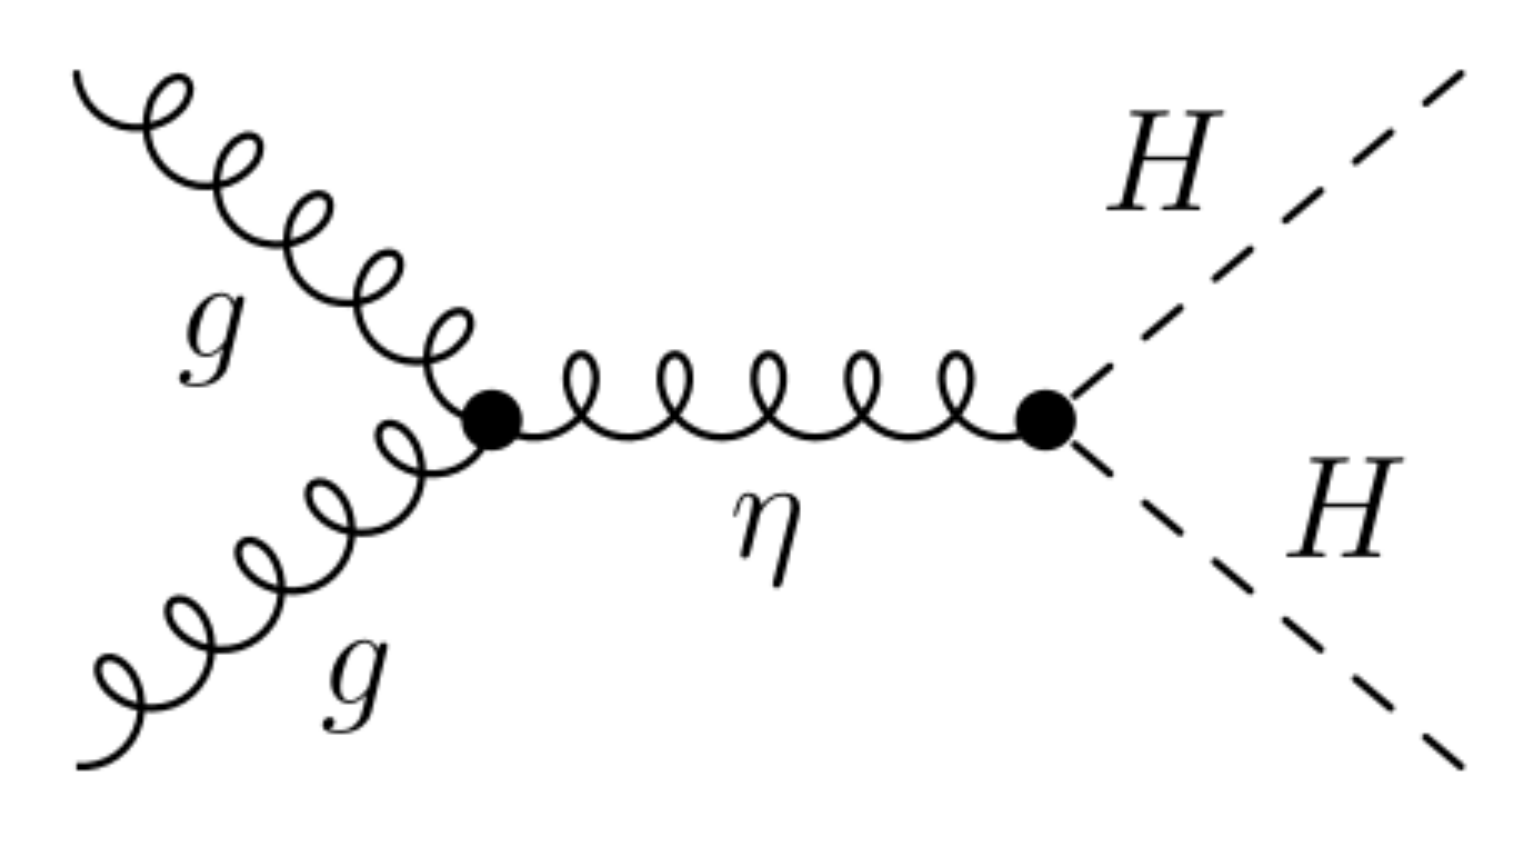
\includegraphics[trim={0cm 0cm 0cm 0cm},clip,width=.7\linewidth]{./Figures/graviton.png}
	\end{minipage}%
	\begin{minipage}{.5\textwidth}
		\centering
		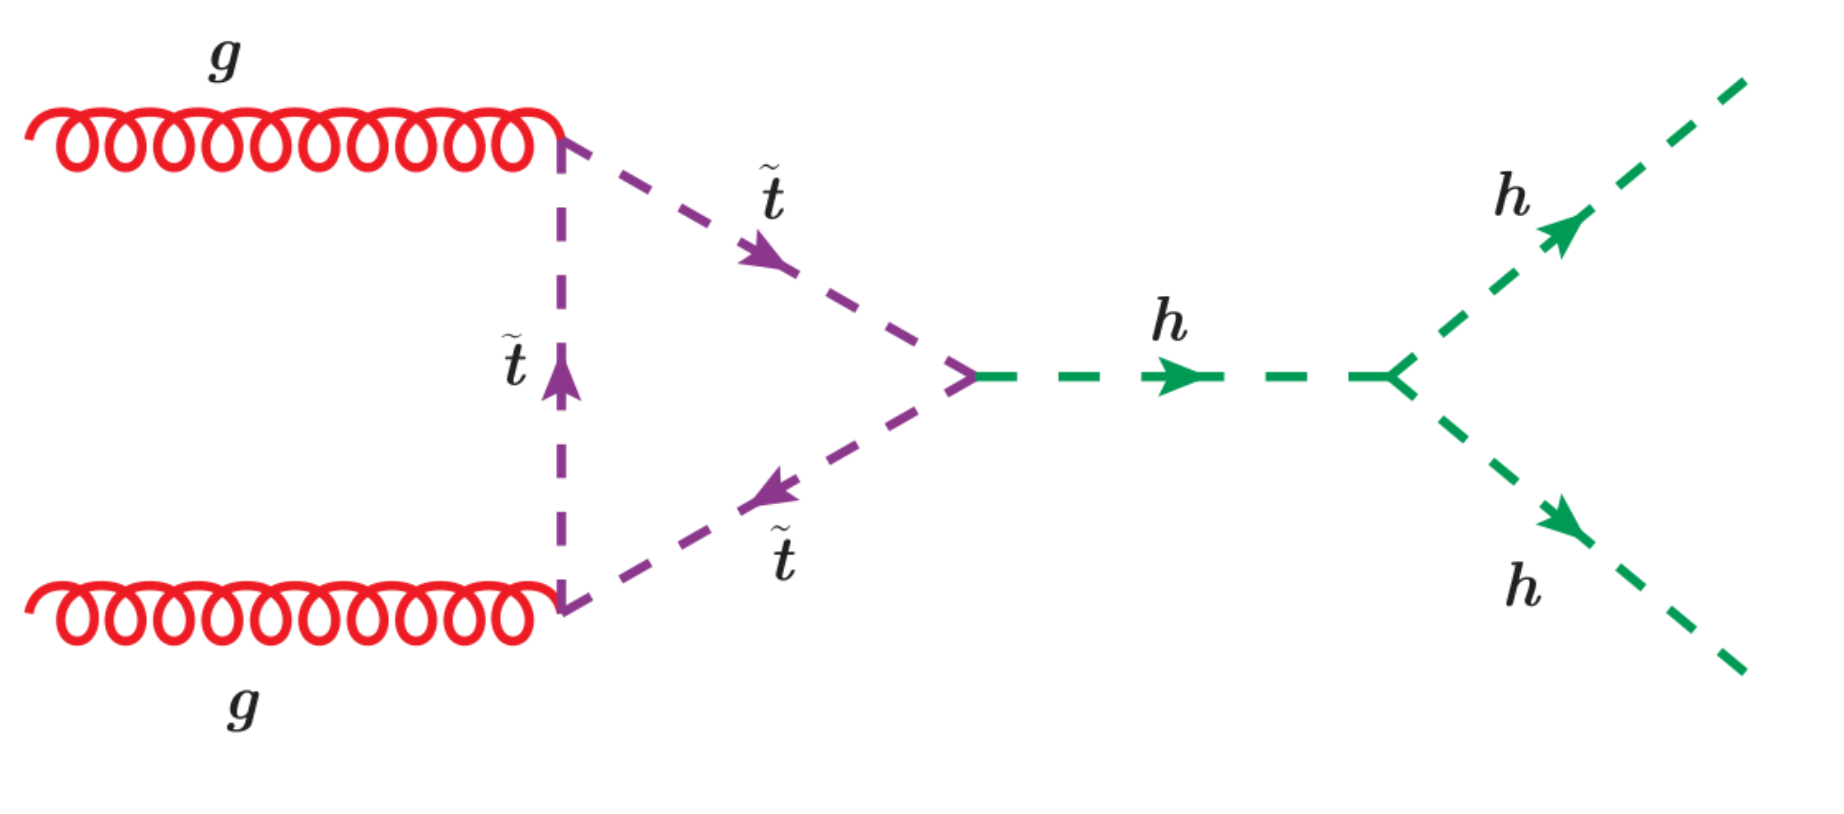
\includegraphics[trim={0cm .5cm 0cm 0cm},clip,width=\linewidth]{./Figures/susy.png}
	\end{minipage}
	\begin{minipage}[t]{0.5\textwidth}
		\caption*{(a)}
		%\label{fig1}
	\end{minipage}%%%
	\hfill
	\begin{minipage}[t]{0.5\textwidth}
		\caption*{(b)}
		%\label{fig2}
	\end{minipage}
	\caption{BSM contributions to Higgs pair production from the spin-2 Kaluza-Klein graviton (a) and from the SUSY partner of the top quark (b). Figures from Refs. \cite{hhBSMgrav,hhBSMsusy}, respectively.}
	\label{fig:BSM_diag}
\end{figure}

%BSM models: \cite{BSM_motivation}\\
%- GUT \\
%- SUSY \\
%- Large extra dimensions (Kaluza-Klein graviton) \\
%- Composite Higgs \\
%- Multi-Higgs 

%%%%%%%%%%%%%%%%%%%%%%%%%%%%%%%%%%%%%%%%%%%%%%%%%%%%%%%%%%%%%%%%%%%%%%%%
 % file "Thesis_Background.tex"
\clearpage

%%%%%%%%%%%%%%%%%%%%%%%%%%%%%%%%%%%%%%%%%%%%%%%%%%%%%%%%%%%%%%%%%%%%%%%%
%                                                                      %
%     File: Thesis_Background.tex                                      %
%     Tex Master: Thesis.tex                                           %
%                                                                      %
%     Author: Andre C. Marta                                           %
%     Last modified :  2 Jul 2015                                      %
%                                                                      %
%%%%%%%%%%%%%%%%%%%%%%%%%%%%%%%%%%%%%%%%%%%%%%%%%%%%%%%%%%%%%%%%%%%%%%%%

\chapter{Collider experiments}
\label{chapter:exp}

In this chapter we start by providing an overview of the goals and main challenges of modern collider experiments. The definitions of some key quantities that describe an accelerator are introduce and a brief discussion on how they influence the discovery potential of an accelerator presented. 

In section \ref{section:LHC} we introduce the LHC and in section \ref{section:ATLAS} we describe the ATLAS experiment, including brief discussions on b-tagging, trigger and data acquisition algorithms and systems. In section \ref{section:jet_reco} we introduce the concept of a hadronic jet and describe how these objects are reconstructed in a general collider experiment. Jet properties and substructure observables, as well as jet grooming algorithms, are introduced in sections \ref{section_jet_sub} and \ref{section:jet_groom}, respectively. 

In section \ref{section:future_colliders} we shift the focus to future collider experiments and accelerators and motivate their need. In sections \ref{section:FCC} and \ref{section:FCC_detector} we introduce the concept of the hadronic Future Circular Collider and describe the baseline detector design, respectively.

Collider experiments are the best tool we have to explore matters' most fundamental structure. 
When we accelerate a particle we increase its momentum. If we take into account the wave particle duality and the De Broglie expression, $\lambda=h/p$, where $\lambda$ is the wavelength and $p$ is the particle's momentum, we can see that a paticle with a large $p$ will have a small $\lambda$. The wavelength gives us the dimension scale of the objects we can probe with a given wave. If we want to probe very small particles (subatomic and smaller) we need very small $\lambda$ and therefore very large $p$. Conceptually, this is the basic idea behind modern particle accelerators. 

In practice, charged particles can be accelerated and their trajectories controlled by means of electromagnetic fields. However, this is not without numerous technical challenges. When a charged particle is subject to an acceleration perpendicular to its velocity (which is exactly what happens in circular accelerators) it emits electromagnetic radiation, called synchrotron radiation. The power emitted is proportional to the fourth power of the particle's energy and inversely proportional to the radius squared and to the fourth power of the particle's mass. This radiation limits the maximum energy that can be achieved in electron-positron colliders. In proton-proton colliders, however, the energy is limited by the maximum magnetic field that can be achieved. Therefore, there is also the need for extremely powerful magnets which are usually implemented using technology based in superconductivity. Using superconducting magnets raises another challenge: they can only operate at very low temperatures, close to the absolute zero. In addition, in order to sustain a stable beam it is necessary that the beam pipe has an environment very close to absolute vacuum.   

\section{Experimental aspects}

One of the most important parameters of a particle accelerator is the time integrated luminosity, $\int \mathcal{L}(t) dt$. For a given process with cross section $\sigma$, it determines the number of event that will be produced, $N$:
\begin{equation}
N=\sigma \int \mathcal{L}(t) dt,
\label{eq:n_events}
\end{equation}
where $\mathcal{L}(t)$ is the instantaneous luminosity that is a measure of the number of collisions per bunch crossing.
The instantaneous luminosity is given by:
\begin{equation}
\mathcal{L}=f_{coll}\frac{n_1 n_2}{4\pi\sigma_x \sigma_y},
\label{eq:inst_lumi}
\end{equation}
where $f_{coll}$ is the collision frequency, $n_1$ and $n_2$ are the number of protons in each bunch and $\sigma_x$ and $\sigma_y$ characterize the transverse beam size in the horizontal and vertical directions.

To increase the chances of measuring a rare process, or to increase the statistical significance of the measurement of an already discovered process, we want to increase $N$ as much as possible. To do so we can either increase the cross section of the process or the integrated luminosity. 

While the cross sections of most physics processes increase when the CM energy goes from $13$ to $100$ TeV, many BSM models predict new processes, or new contributions to existing processes, whose cross sections increase more rapidly than the SM backgrounds. In addition, by conservation of energy, a larger CM energy implies that particles with larger mass can be created. Based on Eq. \ref{eq:inst_lumi}, we can tune its parameters to obtain the highest possible luminosity. Nonetheless, because we are dealing with charged particles, there is a limit on how close the bunches can be and on how many protons we can pack in a bunch. Moreover, the beam's transverse dimensions cannot be infinitely reduced. A smarter way to increase the number of collisions that an accelerator can produce is to run for a longer time, therefore increasing the integration time in Eq. \ref{eq:n_events}. 

In conclusion, the CM energy and the integrated luminosity are two of the main parameters that drive the discovery potential of an accelerator. 

%Therefore these must be carefully analyzed when planning future accelerators.

%%%%%%%%%%%%%%%%%%%%%%%%%%%%%%%%%%%%%%%%%%%%%%%%%%%%%%%%%%%%%%%%%%%%%%%%
\section{The Large Hadron Collider}
\label{section:LHC}

IDEAS FOR SECTION

- The LHC: goals and physics programs \\
- Successes, discoveries \\
- Upgrades and outlook

----------------------------------

The Large Hadron Collider (LHC) is the world's largest and most powerful particle accelerator. It is housed by the European Organization for Nuclear Research (CERN) which focuses on fundamental particle physics with the goal of probing matter's most elementary structure. Ever since its creation, in 1954, CERN has housed many accelerators and experiments and played a key role in the development of fundamental and applied science.

%(DESCREVER MUITO BREVEMENTE ACELERADORES ANTERIORES? SC, SPS, LEP, ...)

The LHC consists of a 27-kilometer ring located beneath the Franco-Swiss border, near Geneva. Most of its running time is dedicate to accelerating protons up to a maximum center of mass energy ($\sqrt s$) of 13 TeV and colliding them at the center of the two general purpose experiments, ATLAS (which is described in section \ref{section:ATLAS}) and CMS. The LHCb experiment also records data from proton-proton collisions but it is dedicated to the study of beauty particles. The ALICE experiment is optimized to study heavy-ion collisions at a CM energy of $2.76$ TeV.

The acceleration of charged particles at the LHC is based on radio frequency (RF) cavities. These cavities are shaped to sustain a resonant electromagnetic field that oscillates at a frequency of 400 MHz. During the acceleration stage, charged particles passing through the cavities feel an overall force that propels them forward. When the LHC is running at full energy, a perfectly timed proton with exactly the right energy feels a zero net force when passing the cavities. Protons with a slightly different energies arriving slightly earlier or later are decelerated or accelerated in order to keep the beam sorted in discrete packages with the same energy. These are called bunches. There are 2808 bunches circulating at the same time, each containing approximately $10^{11}$ protons. The bunches are spaced by 25 ns. Furthermore, the successful operation of the LHC also relies on superconducting magnets made of Niobium-Titanium filaments chilled to $-$271.3$\degree$C and on an ultra high vacuum (of the order of $10^{-10}-10^{-11}$ mbar) inside the beam pipes. The magnets are placed along the LHC ring and produce dipole and quadrapole electromagnetic fields. The dipole magnets create a nominal field of $8.3$ T and bend the beam along the tunel. The quadropole magnets focus the beam at the interaction points. The ultra high vacuum greatly reduces the probability that the beam interacts with any particle. It is crucial to keep a stable beam to continuously maintain collisions during long runs.

%In a hadronic accelerator, the maximum reachable energy is usually limited by its circumference and by the magnetic field strength of the bending magnets. The instantaneous luminosity, $\mathcal{L}$, is a measure of the number of events that the accelerator can produce per bunch crossing. It depends on the frequency of the collisions, $f_{coll}$, on the number of particle in each bunch, $n_1$ and $n_2$, and on how focused the beams are when they collide:
%where $\sigma_x$ and $\sigma_y$ characterize the transverse beam size in the horizontal and vertical directions. Based on \ref{eq:inst_lumi}, we can tune its parameters to obtain the highest possible luminosity. Nonetheless, because we are dealing with charged particles, there is a limit on how close the bunches can be and on how many protons we can pack in a bunch. Moreover, the beam's transversal dimensions cannot be infinitely reduced. A smarter way to increase the number of collisions that a accelerator can produce is to leave running for longer. This does not increase the instantaneous luminosity but it increases the integrated luminosity that is given by $\int \mathcal{L}(t) dt$. 
%By conservation of energy, a larger CM energy implies that particles with larger mass can be created. In addition, while the cross sections of most physics processes increase with the CM energy, many BSM models predict new processes, or new contributions to existing processes, whose cross sections increase more rapidly than the SM backgrounds as a function of the CM energy. When it comes to luminosity, we want it to be as high as possible. More collisions means that we have a higher probability of producing rare processes.  
%As initially described in the letter of intent \cite{ATLAS_letter}, the ATLAS experimental program using proton-proton collisions focuses on the exploration of the Higgs and top quarks sectors in different decay channels, on the measurement of Charge Parity (CP) violation in B mesons decays, on the search for supersymmetry (SUSY), new vector bosons and quark substructure and on the study of gauge boson pair production. 

One of the main research goals of the LHC was to discover the Higgs boson. This was achieved in 2012 when ATLAS and CMS reported the discovery of a particle consistent with the boson predicted by the Higgs mechanism, with a mass of 125 GeV \cite{higgsDiscoveryATLAS},\cite{higgsDiscoveryCMS}. Ever since, efforts have been directed to measuring its mass, couplings, spin-parity properties with increasing precision using different decay channels and production modes. 

ATLAS and CMS reported evidence (measurement with a significance greater than three sigma) for the Higgs decaying to $b\overline{b}$ \cite{h2bb, CMSh2bb} [UPDATE WITH DISCOVERY]. The searches targeted the $VH$ production mode. It offers the best sensitivity to the $hb\bar{b}$ Yukawa coupling because requiring a vector boson helps reduce the SM backgrounds, namely the ones from QCD interactions. CMS reported the first observation (measurement with a significance greater than five sigma) of the Higgs boson decaying to a pair of tau leptons \cite{CMSh2tautau}. In addition, the observation of Higgs boson production in association with a $t\overline{t}$ pair was very recently reported by both collaborations \cite{CMStth, ATLAStth}. Moreover, precision measurements of the masses of the Higgs \cite{ATLAShMass,hMass} and $W$ \cite{ATLASwMass} bosons and of the top quark \cite{ATLAStopMass, CMStopMass} were also performed. 
So far, no conclusive signs of new physics were seen at the LHC.
%Other LHC results:\\
%- h to bb (evidence) ATLAS+CMS \\
%- h to tau tau (discovery) CMS \\
%- ttH (discovery) ATLAS+CMS \\
%- t production in proton-lead collisions (CMS) ? \\
%- Precision measurements: top, W and Higgs mass \\
%- LHCb results: lepton universality, 5 new particles, ... ? \\
%- No conclusive signs of new physics; constrain models

Future prospects for the LHC include its upgrade to the High Luminosity-LHC (HL-LHC) after
the scheduled long shutdown of 2024-2026. This upgrade will increase the size of the dataset to $3000~\text{fb}^{-1}$ over the course of ten years \cite{High-Luminosity}. 
During the shutdown, the ATLAS detector will be upgraded. 

%MAIN UPGRADES (namely, refer TileCal high granularity upgrade ?)

%HL-LHC physics programme:\\
%- Higgs precision measurements (properties and couplings) \\
%- Higgs rare processes: h to mu mu, h to J/Psi \\
%- Higgs self couplings \\
%- BSM searches: SUSY, 2HDM, ...\\

In the Higgs sector, the high value of the integrated luminosity will improve the statistical precision of already measured channels and the discovery potential of rare processes \cite{HL_LHC}.

\subsection{The ATLAS detector}
\label{section:ATLAS}

The ATLAS detector has a cylindrical geometry and a multi layered structure. Its dimensions are 25 meters in height (diameter) and 44 meters in length and it weights approximately 7000 tonnes. In the following paragraphs we describe the detector's layers and their functionalities. A schematic representation of the detector as well as the appropriate coordinate system can be found in figure \ref{fig:ATLAS_detector}.

A combination of cartesian and cylindrical coordinates is used to describe the detector. In both cases, the origin is defined to coincide with the interaction point. The Cartesian system is right-handed and the z axis is defined to be the direction of the beam. The x-axis point from the interaction point to the center of the LHC ring and the y-axis point upwards. The azimuthal angle, $\phi$, is measured around the beam axis and the polar angle, $\theta$, from the beam line. The pseudorapidity is defined as $\eta=-\ln \tan(\theta/2)$. Another commonly used quantity is the rapidity, $y$, defined as a function of a particle's energy, $E$, and longitudinal momentum, $p_L$: $y=\frac{1}{2}\ln \left(\frac{E+p_L}{E-p_L}\right)$. In the limit where a particle's mass is negligible with respect to its momentum the pseudorapidity converges to the definition of rapidity. In addition, the angular distance between two points, $\Delta R$, is defined as $\Delta R=\sqrt{(\Delta \phi)^2+(\Delta \eta)^2}$, where rapidity can also be used instead of the pseudorapidity. 

The detector consists of an inner detector (ID) or tracker, electromagnetic (EM) and hadronic calorimeters and a muon spectrometer (MS).
The magnet configuration consists of a thin superconducting solenoid that surrounds the ID cavity and three superconducting toroids (one barrel and two end-caps) arranged with an eight-fold azimuthal symmetry around the calorimeters.

The ID covers the pseudorapidity range $|\eta|<2.5$ and it makes up the innermost layer of the detector. It consists of silicon pixel, silicon micro-strip, and straw tube transition radiation tracking detectors. It is contained in a solenoid magnet with a central field of $2$ T. The tracker provides precision measurements of the positions and momenta of charged particles. As a charged particle transverses the several layers of the ID it ionizes the medium creating electrical signals that can be read out. These individual electrical signals are then combined to reconstruct the trajectory of the particle. 

Lead/Liquid-Argon (LAr) sampling EM calorimeters cover the pseudorapidity range $|\eta|<3.2$. The EM calorimeter has an accordion like structure with layers of showering material (lead) interleaved with layers of active material (liquid argon). These calorimeters provide measurements of the energy of electrons and photons. The interaction of these particles with the lead layers induces the production of an EM shower whose energy  is measured in the liquid argon layers. The granularity of the EM calorimeter strongly depends on the longitudinal layer and on the pseudorapidity region. 

The hadronic calorimetry in the pseudorapidity range $|\eta|<1.7$ is provided by a scintillator-tile calorimeter (TileCal) which is divided in a central barrel and two smaller end-cap barrels, one on each side of the central barrel. The active components are scintillator tiles made of polystyrene that are interleaved with steel plates as the passive material. The scintillation light emitted by the tiles when an ionising particle crosses the calorimeter is collected on both ends of the tiles by wavelength-shifting optical fibers. The light signal emitted is proportional to the particle's energy. The TileCal is composed of several cells with transverse segmentation $\Delta\eta\times\Delta\phi=0.1\times0.1$ \footnote{The TileCal is composed of three longitudinal layers. Only the first two have a segmentation equal to $0.1\times 0.1$. In the third layer the segmentation is $0.2\times 0.1$. However, most of the energy of hadronic showers is deposited in the first layers and therefore this detail is not very relevant for this work.} \cite{TileCalTech}. 

For $|\eta|>1.5$ LAr calorimeters extend the pseudorapidity range to $|\eta|=4.9$. The LAr calorimeter is divided in end-cap and forward. These cover the pseudorapidity ranges $1.5<|\eta|<3.2$ and $3.2<|\eta|<4.9$, respectively. The active material is liquid-argon and the absorbers are copper and tungsten for the end-cap and forward calorimeters, respectively. In the end-cap LAr calorimeters the segmentation is $\Delta\eta\times\Delta\phi= 0.1\times0.1$ for $1.5<|\eta|<2.5$ and $0.2\times0.2$ for $2.5<|\eta|<3.2$. In the forward LAr calorimeter the segmentation is $\Delta\eta\times\Delta\phi= 0.2\times0.2$. 

The granularity of the ATLAS hadronic calorimeters is summarized in table \ref{table:ATLAS_HCAL}.

\renewcommand{\arraystretch}{1.2}

\begin{table}
	\centering
	\begin{tabular}{llll}
		\toprule 
		\textbf{TileCal} & \textbf{Barrel} & \textbf{Extended barrel} &\\
		\midrule
		Coverage & $|\eta|<1.0$ & $0.8<|\eta|<1.7$  & \\
		Granularity & $0.1\times 0.1$ & $0.1\times 0.1$ & \\
		\midrule \midrule
		\textbf{LAr calorimeter} & \textbf{End-cap} & \textbf{Forward} &\\
		\midrule
		Coverage & $1.5<|\eta|<3.2$ & $3.2<|\eta|<4.9$  &  \\
		\multirow{2}{*}{Granularity} & $0.1\times 0.1 ~\text{for}~ 1.5<|\eta|<2.5$ & \multirow{2}{*}{$0.2\times 0.2$} & \\
		& $0.2\times 0.2 ~\text{for}~ 2.5<|\eta|<3.2$ & & \\
		\bottomrule
	\end{tabular}
	\caption{ATLAS tile and liquid argon hadronic calorimeters: summary of the pseudorapidity coverages and transversal segmentation (granularity).}
	\label{table:ATLAS_HCAL}
\end{table}

The hadronic calorimeters provide measurements of the energy of hadrons, jets, $\tau$ leptons and missing transverse energy $\left(E_T^{miss}\right)$. Approximately one third of the energy of jets is deposited in this layer. In the TileCal, the jet energy resolution is given by $\sigma/E\sim 50\%/\sqrt{E}+3\%$ \cite{TileCalTech},
where the first term is the stochastic term that derives from sampling fluctuations and follows a Poisson distribution and the second term is a constant that depends on the characteristics of the calorimeter. For the LAr calorimeter, the jet energy resolution is given by $\sigma/E\sim 60\%/\sqrt{E}+2\%$ \cite{ATLAS_LAr_TDR}.

The MS is the outermost layer of the detector and it is dedicated to detecting muons that travel through the previous layers almost without interacting. This layer provides measurements of the muons transverse momenta. It is composed of Monitored Drift Tubes (MDT) and Cathode Strip Chambers (CSC) that provide high precision measurements of the muons' momentum in the pseudorapidity range $|\eta|<2.7$ and of Resistive Plate Chambers (RPC) and Thin Gap Chambers (TGC) dedicated to triggering purposes for $|\eta|<2.4$.

\begin{figure}
	\centering
	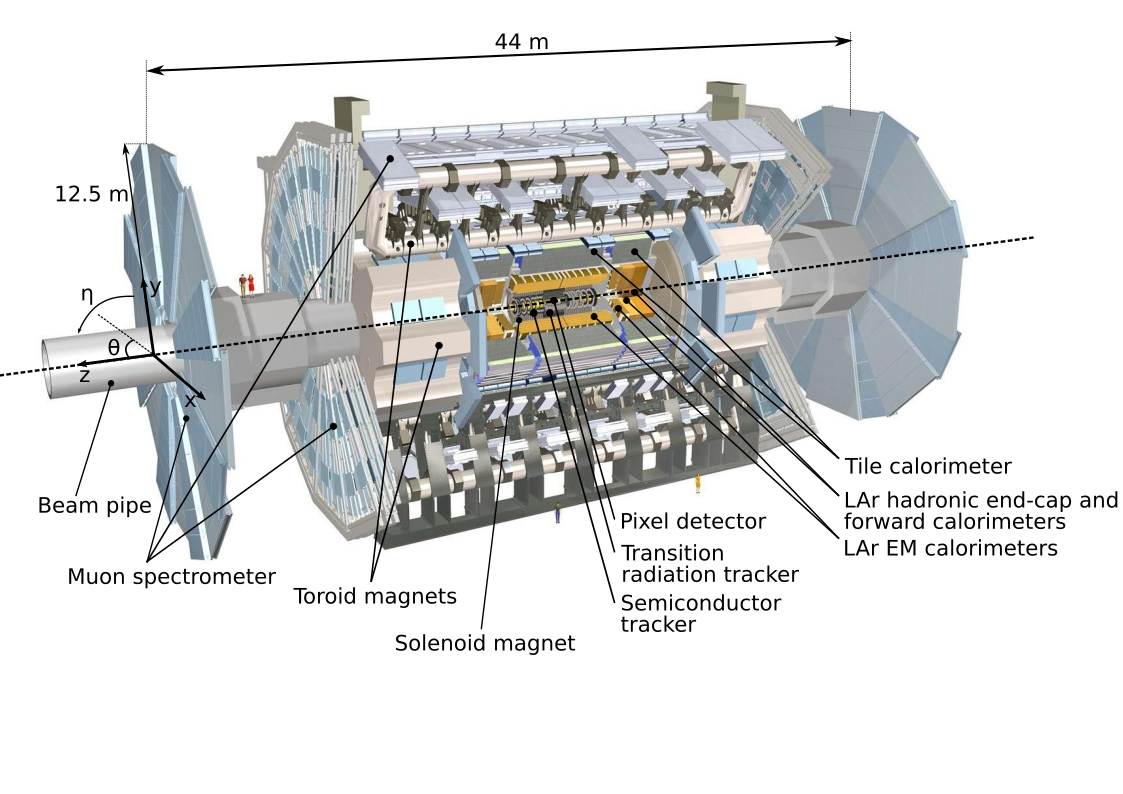
\includegraphics[trim={0cm 3.5cm 0cm 0},clip,width=\textwidth]{./Figures/ATLASsvg3.png}
	\caption{ATLAS detector.}
	\label{fig:ATLAS_detector}
\end{figure} 

\subsubsection{b-Tagging}

Each collision produces a large number of hadronic jets (we refer to section \ref{section:jet_reco} for a detailed description of jets and how they are reconstructed). For this work, jets initiated by a b quark (b jets) are particularly important: we are looking for a Higgs pair decaying to four b quarks which leads to an experimental signature that consists of four b-jets. b-Tagging algorithms determine, with a given probability, if a jet was originated by a b quark. 

When a b quark is produced it hadronizes almost instantly, producing a B hadron. B hadrons have a life time of $\sim$ 1 ps and can be highly relativistic meaning that they can travel a few millimeters to a few centimeters inside the inner detector before decaying. When they decay there is often a reconstructible secondary vertex that is slightly displaced from the primary vertex where the b-quark was produced. The existence of a secondary vertex is used by b-Tagging algorithms to identify, or tag, a jet as coming from a b-quark. It is important to note that a complete b-tagging algorithm relies on the reconstruction of a secondary vertex which can only be done using the information form the inner detector. This implies that, in ATLAS, we can only b-tag jets that are produced in the region $|\eta|<2.5$.

In ATLAS, b tagging algorithms are applied to the sub-set of tracks that are associated with that jet. The matching between tracks and calorimeter-based jets is performed using the ghost association technique \cite{GhostAssociation}\footnote{This procedure works by introducing ghost versions of the measured tracks that have the same direction but infinitesimally small $p_T$ such that they do not modify the properties of the calorimeter jets. The jets are then reclustered and a track is considered to be associated with a given jet if its ghost version is contained in the jet after reclustering.}. The identification of b-jets in ATLAS is based on distinct strategies encoded on three b-tagging algorithms: impact parameter-based algorithms, an inclusive secondary vertex reconstruction algorithm and  a decay chain multi-vertex reconstruction algorithm. The output of these algorithms are combined in a multivariate discriminant based on a Boosted Decision Tree (BDT) which provides the best discrimination between the different jet flavors \cite{btagATLAS}.

The impact parameter-based algorithms, IP2D and IP3D, use as discriminant variables the transverse impact parameter significance and the transverse and longitudinal impact parameter significance, respectively. The secondary vertex finding algorithm, SV, explicitly reconstructs a displaced secondary vertex inside the jet by trying to find pairs of tracks with a common origin. The decay chain multi-vertex reconstruction algorithm, JetFitter, tries to reconstruct the full b-hadron decay chain. This approach allows to resolve b- and c-hadrons vertices even if there are not two tracks associated with them.

\subsubsection{Trigger and data acquisition}

The LHC delivers approximately 1000 million proton-proton collisions per second, which corresponds to an event rate of 1 GHz. On the one hand, only a small fraction of these events result in interesting physics processes. On the other hand, the detector does not have enough storage and read out capabilities to record all the collisions. The triggering and data acquisition systems are responsible for selecting a manageable rate of events for permanent storage and further analysis. 

The trigger is responsible for selecting events with interesting experimental signatures. The trigger system in Run-2 consists of a hardware-based first  level  trigger (Level-1) and a software-based high level trigger (HLT). The Level-1 trigger takes as input  coarse  granularity calorimeter and muon detector information and reduces the event rate to 100 kHz. The HLT uses full granularity detector information and reduces the rate to approximately 1 kHz \cite{run2trigger}.    

[USE ANOTHER EX?] Take, as an example, the inclusive cross section for the production of jets which is of the order of $10^6$ fb. If we consider a luminosity of $0.8~\text{fb}^{-1}$ per day, this corresponds to a rate of approximately 200 Hz, just for the production of jets. Note that this value is the same as the maximum allowed rate for all physics processes after all the triggers. Therefore, it is clear that we cannot simply take all the jet events. We need to place tight cuts that allow us to reduce this rate to an acceptable (within the available quotas) rate. This is of particular importance for processes with very large cross sections such as QCD multijet production.

%\begin{figure}[!tbp]
%	\centering
%	\begin{minipage}[b]{0.4\textwidth}
%		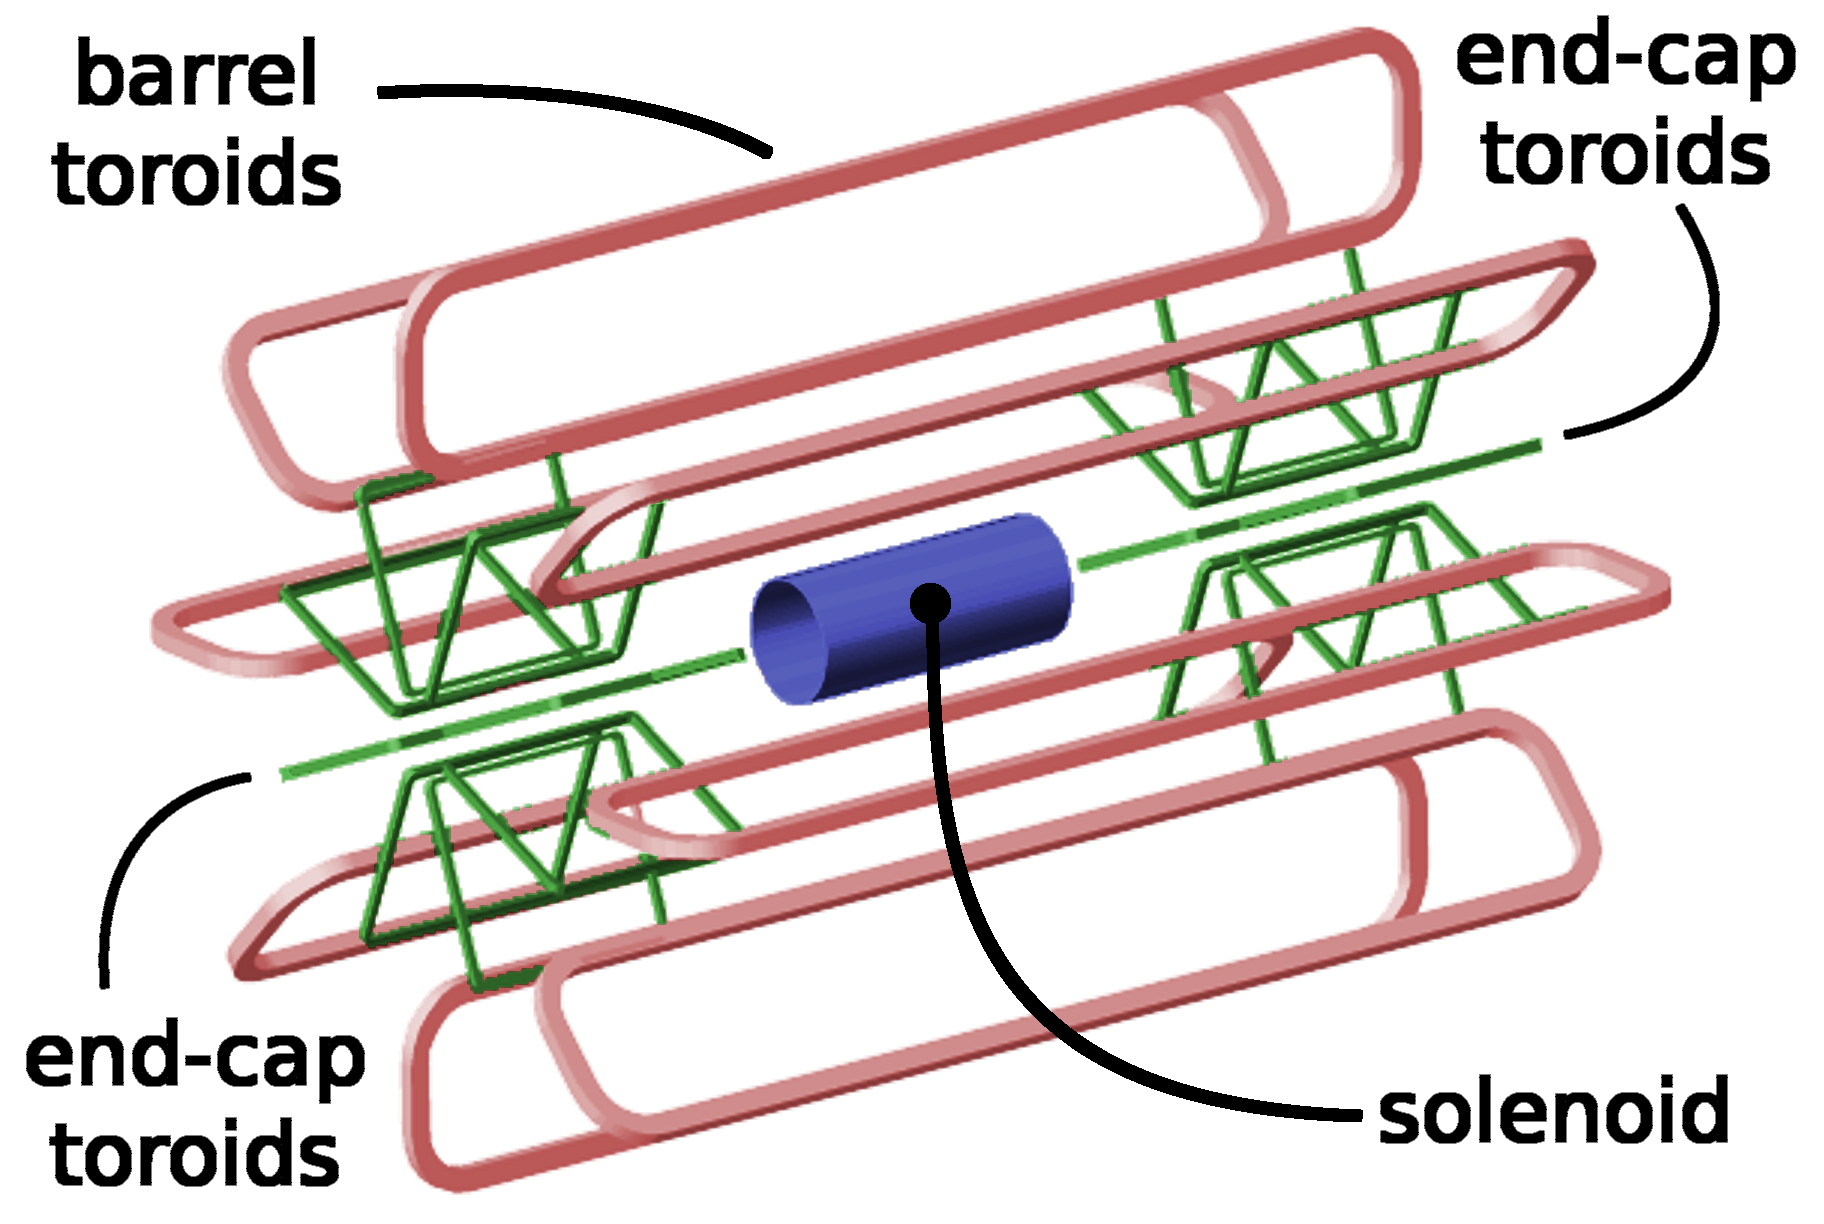
\includegraphics[width=\textwidth]{./Figures/magnetSystems.png}ing system 
%		\caption{Flower one.}
%	\end{minipage}
%	\hfill
%	\begin{minipage}[b]{0.4\textwidth}
%		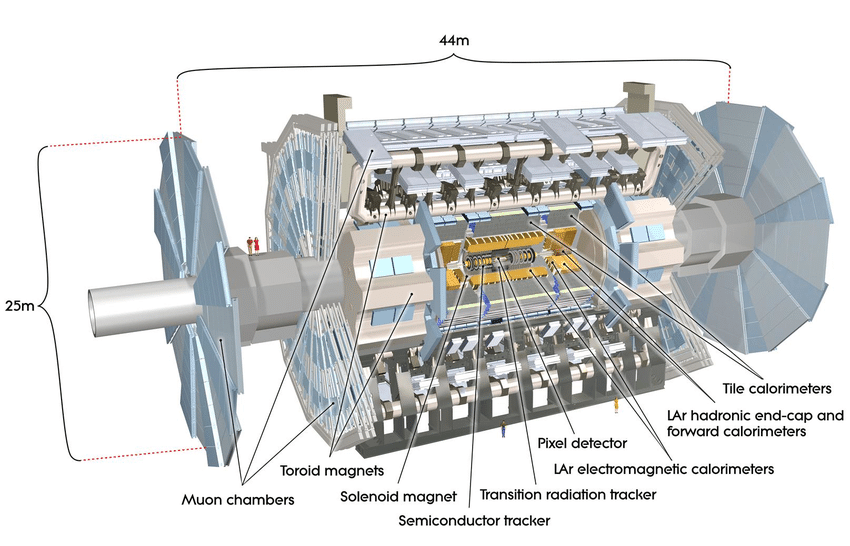
\includegraphics[width=\textwidth]{./Figures/ATLAS.png}
%		\caption{Flower two.}
%	\end{minipage}
%\end{figure}

%\begin{figure}
%	\centering
%	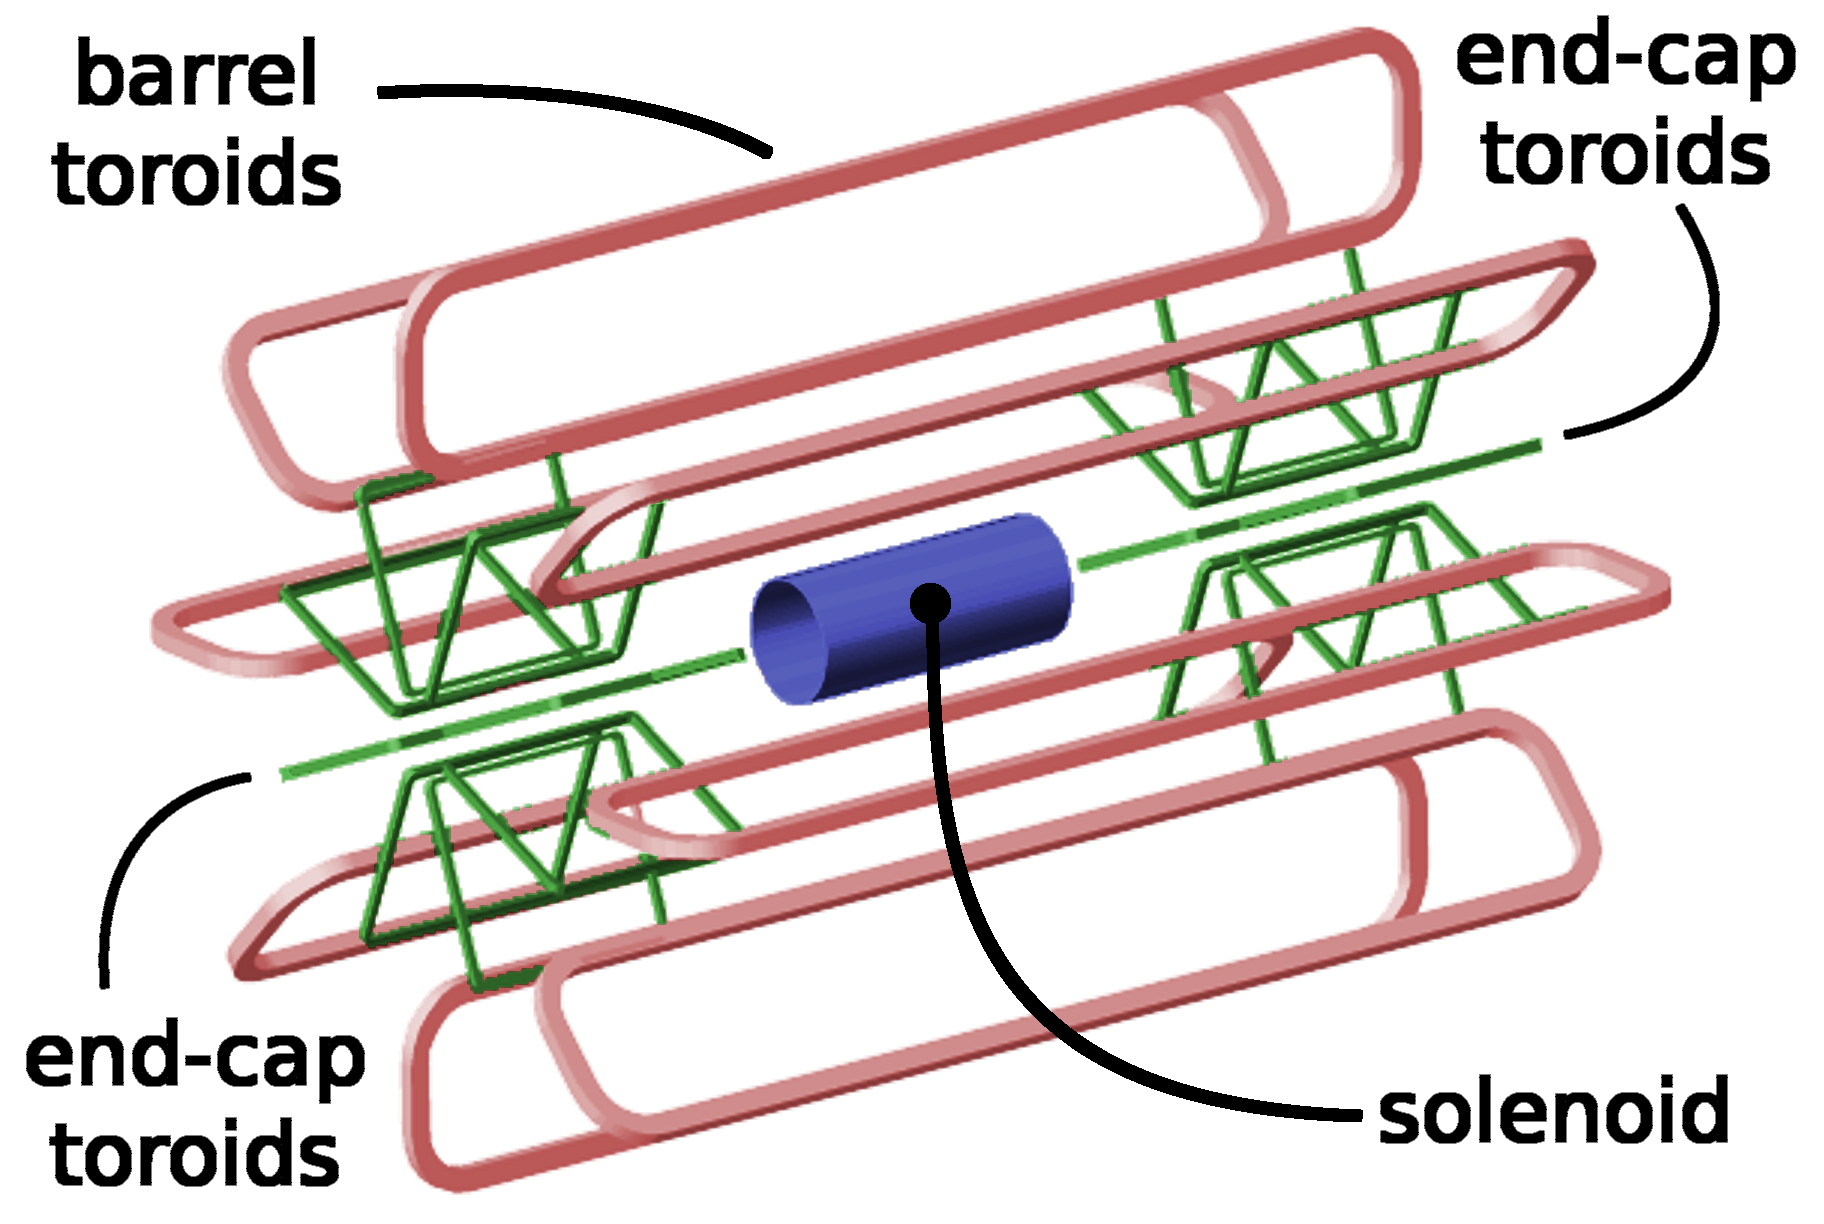
\includegraphics[width=0.5\textwidth]{./Figures/magnetSystems.png}
%	\caption{ATLAS detector magnet configuration.}
%	\label{fig:ATLAS_magnet}
%\end{figure}     

%%%%%%%%%%%%%%%%%%%%%%%%%%%%%%%%%%%%%%%%%%%%%%%%%%%%%%%%%%%%%%%%%%%%%%%%

\section{Jet reconstruction}
\label{section:jet_reco}

A jet is a collimated spray of hadrons that is interpreted as coming from a single initial parton such that it approximately retains information about its physical properties, namely 3-momentum, mass and charge. The existence of such objects is a direct consequence of the confinement property of Quantum Chromodynamics (QCD). Quarks and gluons, the fundamental degrees of freedom of QCD, are not asymptotically free. They are confined inside hadrons. Therefore, when one of these particles is produced it undergoes showering and hadronization processes that lead to the formation of hadrons.

At a particle detector we are interested in reconstructing jets. These are the objects that are used in the physics analysis. Working with jets instead of hadrons is an advantage because it greatly reduces the number of objects we need to analyze per event. In addition, they work as a \textit{proxy} for the fundamental partons produced in the event.

Jets are obtained through jet finding algorithms. These are clustering algorithms that group together experimental quantities (energy deposits in the calorimeters, tracks or particle flow objects) using a sequential recombination scheme. A crucial property of these algorithms is that they should be infrared and collinear safe, meaning that the outcome of the algorithm (namely the number of jets and their properties) should not be significantly
modified by the emission of soft radiation or by a collinear splitting.

The most widely used jet finding algorithms are the $k_T$ \cite{kt}, the Cambridge/Aachen (C/A) \cite{CA} and the anti-$k_T$ \cite{anti-kt}. They are based on distance measurements:

\begin{equation}
d_{ij}=\min(k_{Ti}^{2p},k_{Tj}^{2p})\frac{\Delta_{ij}^2}{R^2}, \qquad
d_{iB}=k_{Ti}^{2p},
\end{equation}
where $d_{ij}$ is the distance between entities $i$ and $j$ and $d_{iB}$ is the distance between entity $i$ and the beam ($B$). $\Delta_{ij}^2=(y_i-y_j)^2+(\phi_i-\phi_j)^2$ and $k_{Ti}$, $y_i$ and $\phi_i$ are the transverse momentum, rapidity and azimuth of entity $i$. Here, $k_{T}$ stands for the transverse momentum. For $p=1,0,-1$ we get the $k_T$, C/A and anti-$k_T$ algorithms, respectively.

The clustering algorithm starts by computing all $d_{ij}$ and $d_{iB}$ distances. If the smallest distance is a $d_{ij}$, the four momenta of particle $i$ and $j$ are summed and the distances are updated. If the smallest distance is a $d_{iB}$, particle $i$ is removed and called a jet. This procedure is iterated until all particles are clustered in jets.

It is worth discussing further the anti-$k_T$ algorithm since it is the default algorithm used in most analyses, including this one. In this algorithm, the $\Delta_{ij}$ distance between constituents $i$ and $j$ is weighted by the inverse of the transverse momentum of the constituent with a largest $k_T$. This feature implies that particles with larger momenta will have a smaller $d_{ij}$ distance and therefore will be clustered first. This prevents soft particles from being clustered among themselves before clustering the hardest particles.

In ATLAS, the transverse and longitudinal segmentation of the calorimeters allow for a three dimensional reconstruction of particle showers which is based in a topological clustering algorithm. Topo-clusters of calorimeters cells are seeded by cells whose absolute energy exceeds the electronic and pile-up noise by four standard deviations. The topo-clusters are then expanded by adding all adjacent cells with absolute energy two standard deviations above noise. Finally, all cells neighbouring the previous set are also added. After energy calibration, the topo-clusters are fed as input to a jet finding algorithm.  

\subsubsection{Boosted kinematic regime}

With the increase of the CM energy of particle colliders the production of particles with a transverse momentum much larger that their mass became a reality. In this kinematic regime (referred to as boosted due to the high Lorentz boost of the particles) traditional jet reconstruction algorithms, that rely on a one-to-one correspondence between jets and partons, begin to fail \cite{jetsubLHC}. 

Due to the high Lorentz boosts, decay products of heavy resonances get more collimated. The angular separation of the decay products is approximatelly \cite{jetsub}:
\begin{equation}
	\Delta R \sim \frac{2 m}{p_T}
	\label{eq:deltaR}
\end{equation}
where $p_T$ and $m$ are the transverse momentum and mass of the decaying particle. In addition to decaying particles with a larger $p_T$, another event topology that can produce highly collimated particles is the decay of a particle with a very large mass (directly seen from \ref{eq:deltaR}). This scenario is of particular interest for new physics searches because BSM models often predict the existence of heavy particles. 

Take, as an example, the decay of a Higgs boson to two b quarks. Considering that the $p_T$ of the Higgs is approximately $200$ GeV (which is a reasonable and commonly used value in boosted Higgs bosons searches) we get $\Delta R \sim 1$. For resolved jets, the default jet radius parameter used in ATLAS is $0.4$. We see that for a $p_T \sim 200$ GeV the angular separation between the decay products of a Higgs boson is already similar to the default jet diameter, which can jeopardize the ability to resolve the individual decay products.

%There is a limit after which it is no longer possible to reconstruct both decay products as individual jets because the $\Delta R$ between the decay products has a value that is very close to the jet's diameter such that we start to have an overlap between the two jets (?).

A possible workaround is to use a single jet with a larger $R$ parameter to reconstruct both decay products. The problem with doing so is that we no longer have information about each individual decay product which means we are loosing some information about the event. We cannot, for example, compute angular variables between the decay products. This led to the development of techniques and observables that allow for the exploration of the intrinsic structure (or substructure) of these large-$R$ jets. Some of these techniques are introduced and discussed in the following section.  

\subsection{Jet properties and substructure observables}
\label{section_jet_sub}

TO INCLUDE (it will depend on the ones that are most important to the analysis):\\
- tau\_N \\
- energy correlation functions and ratios \\
- Fox Wolfram\\
- ...\\
- Jet mass definition!\\
--------------------------------------------------------------------------------\\

%Perhaps the most used jet observable is the invariant mass, $M$, that is  calculated from the energies and momenta of its constituents as follows:
%\begin{equation}
%	M=\left(\sum_{i}E_i\right)^2-\left(\sum_{i}\vec{p}_i\right)^2
%\end{equation}
%where $E_i$ and $\vec{p}_i$ are the energy and three-momentum of the $i^{th}$ constituent. If we are dealing with large-R jets, the mass can be used as an approximation of the resonances's mass. 

In general, jet substructure variables aim to quantify the existence of energy clusters  insider a jet. Each cluster is interpreted as corresponding to an individual jet. These are called subjets because they are contained inside the large-$R$ jet that was actually reconstructed. Once they are identified, the subjets can be handled and used for the analysis like normal jets. However, a lot of the substructure techniques do not focus on reconstructing the subjets but rather on determining whether or not they exist, how many they are and how are they distributed inside the large-$R$ jet. 

Heavy resonances decaying to two(three) particles will produce large-$R$ jets that are consistent with the existence of two(three) energy clusters. Examples of such topologies are the Higgs and top decays: the Higgs boson always decays to pairs of particles (leptons, quarks or bosons) and the top quark decays, with a probability close to $100\%$, to a $b$ quark and a $W$ boson that then decays to a pair of leptons or quarks. These topologies are usually referred to as two or three prong. In contrast, jets initiated by a gluon or quark splitting are not expected to have a meaningful substructure. The energy is expected to be concentrated around the jet axis following an isotropic distribution and to become less dense as we approach the jet's border. This is the signature of a one-prong topology. The previous discussion is valid at LO and captures the generic features of jets that are targeted by jet substructure techniques. Nonetheless, other effects may come into play. Take, for example, a highly virtual gluon with a high $p_T$. If it splits into two quarks the resulting jet may have two subjets and thus mimic the topology of a heavy resonance decay.

The N-subjetiness variable \cite{Nsubjetiness}, $\tau_N$, may be used to identify jets compatible with N subjets. It is given by 
\begin{equation}
	\tau_N = \frac{1}{d_0}\sum_{k}p_T^k \min(\Delta R_1^k,...,\Delta R_N^k), \qquad d_0=\sum_{k}p_T^k R_0
\end{equation}
where the index $k$ runs over all particles in a jet, the indexes $1$ to $N$ identify the number of axis inside the jet and $R_0$ is the radius of the jet. This variable will have a small value if the particles with the highest $p_T$ (the ones we are most interested in) are clustered around the axis (because $\Delta R$ will be small) and will have a larger value otherwise. A jet with small $\tau_N$ is considered to be consistent with having $N$ or fewer subjets because all its constituents are aligned with the axis.

We usually use ratios of $\tau_N$ variables ($\tau_{MN}=\tau_M/\tau_N$). Of particular interest for this work are the $\tau_{21}$, $\tau_{31}$ and $\tau_{32}$ ratios. These observables can take values between zero and one. For $\tau_{21}$, for example, a small value (close to zero) indicates that the jet is more compatible with two subjets than with one and therefore it can help discriminate between two-prong and one-prong jets. The same applies to every other ratio. 

The Fox-Wolfram moments, $H_l$, can be used to identify jets that have a structure of two back-to-back subjets in their rest frames \cite{FW2}. They are given by:
\begin{equation}
H_l = \sum_{i,j}\frac{|\vec{p}_i||\vec{p}_j|}{E^2}P_l(\cos(\theta_{i,j}))
\end{equation}  
where $\theta_{ij}$ is the angle between energy clusters i and j, $E$ is the total energy of the clusters in the jet rest frame, the $P_l(x)$ are the Legendre polynomials. For a jet that has a structure of two back-to-back subjets in its rest frame, $H_1 = 0$, $H_l \sim 1$ for even l, and $H_l \sim 0$ for odd l. This is what we expect for jets coming from the decay of a boosted resonance. In this work we make use of $H_2$.

In addition to jet substructure observables, more standard variables, from which we highlight the jet mass, can also be used to discriminate between jets coming from QCD background and jets resulting from heavy resonance decays. In the latter, the jet's invariant mass should roughly correspond to the mass of the resonance. The invariant mass of a jet, $M$, is  calculated from the energies and momenta of its constituents as follows:
\begin{equation}
	M=\left(\sum_{i}E_i\right)^2-\left(\sum_{i}\vec{p}_i\right)^2
\end{equation}
where $E_i$ and $\vec{p}_i$ are the energy and three-momentum of the $i^{th}$ constituent. However, the mass resolution is not expected to be very good for large-R jets because of all the extra QCD radiation that may be caught inside the jet. A possible workaround is the use of jet grooming algorithms which we describe in the following section.

\subsection{Jet grooming algorithms}
\label{section:jet_groom}

The main goal of jet grooming algorithms is to remove contamination of softer jet constituents from pileup or underlying event and to leave behind the hard substructure. The main advantage of such algorithms is that they improve the mass resolution of jets. These features are of particular interest in high luminosity environments such as the HL-LHC and future high energy colliders. 

There are three main jet grooming algorithms: trimming, pruning and mass drop filtering. In this work we do not use pruning or trimming, although these techniques might be worth exploring in future, more comprehensive, studies. In particular, they can be useful to help reject pileup contributions. The mass drop filtering procedure isolates relatively symmetric subjets within a jet, each with a significantly smaller mass than the original jet \cite{jetsub}. This technique was developed and optimized using C/A jets for the search of Higgs decaying to $b\overline{b}$ pairs \cite{BDRS}. It works as follows:
\begin{itemize}
	\item The last step of the C/A clustering is undone such that the jet is split in to subjets, $j_1$ and $j_2$ with $m_{j_1}>m_{j_2}$. We require that there is a significant between the mass of the original jet, $m_{\text{jet}}$, and $m_{j_1}$: $m_{j_1}/m_{\text{jet}} < \mu_{\text{frac}}$, where $\mu_{\text{frac}}$ is a parameter of the algorithm. In addition the splitting is required to be relatively symmetric:
	\begin{equation}
		\frac{\min[(p_T^{j_1})^2,(p_T^{j_2})^2]}{(m_{\text{jet}})^2} \times \Delta R_{j_1,j_1}^2 > y_{\text{cut}}
	\end{equation}
	where $y_{\text{cut}}$ is a parameter that defines the energy sharing between the subjets. It is usually taken to be $\sim 0.09$. If these two criteria are not met the jet is discarded.
	
	\item The subjets are clustered with the C/A algorithm with radius parameter $R_{\text{filt}}=\min[0.3,\Delta R_{j_1,j_2}/2]$. All jet's constituents that are outside of the three hardest subjets are discarded and we obtained the filtered jet and its subjets.
\end{itemize}

The subjets that are identified within a jet are interpreted as corresponding to the decay products of the particle that produced the original jet. There are usually only two decay products. A third subjet is allowed in order to account for extra QCD radiation.

\section{Future Colliders}
\label{section:future_colliders}

As we already argued in the beginning of this chapter, a larger CM energy is one of the factors driving the discovery potential of an accelerator. As far as we know today, proton-proton colliders are the main, and possibly only, man-made experimental tool available to explore particle physics in the energy range on tens of TeV. With this in mind, new hadronic colliders with CM energies of the order of tens of TeV have been proposed. The main projects are the hadronic Future Circular Collider (FCC-hh) lead by CERN and the Super Proton-Proton Collider (SPPC) proposed by China. 

In this work we focus on FCC-hh and use the established detector's baseline design as our starting point for this study. In the following section we describe in detail the FCC-hh accelerator and detector.

\subsection{The hadronic Future Circular Collider}
\label{section:FCC}

IDEAS FOR SECTION

- Center of mass energy \checkmark \\
- Basic design: circular, circumference, location, ... \checkmark\\
- CERN FCC study group: creation, mission, main tasks \checkmark \\
- The role of the hadronic calorimeter \\
- Basic structure: tracker, calorimeters, muon chambers \checkmark \\
- Technical specifications: nb. bunches, magnets, ... \checkmark\\
- Technical dimensions and materials (predictes) of each layer \checkmark\\
- Focus on hadronic calorimeter: material being studied, resolution, granularity \checkmark\\
- What processes we want to study at the FCC \\
- Focus on Higgs pair production \\

-------------------------------------------------------------------------------

CERN's FCC study group was launched as a result of a recommendation made in the  2013 update of the European Strategy for Particle Physics that '\textit{Europe needs to be in a position to propose an ambitious post-LHC accelerator project at CERN by the time of the next Strategy update}'. It investigates the technological challenges and physics opportunities of a future circular collider. The design and infrastructure are driven by a proton-proton collider (FCC-hh) requirements. Electron-positron (FCC-ee) and electron-proton (FCC-eh) colliders are also being analyzed. The main goal of this effort is to deliver a Conceptual Design Report (CDR) by the end of 2018. This document will include a first cost estimate to be submited for the next update of the European Strategy for Particle Physics, foreseen by 2018.

The FCC-hh baseline design consists of a proton-proton circular collider with a maximum CM energy of 100 TeV housed by a 100 km tunnel in the area of Geneva. This machine will extend the research program of the LHC (and of the HL-LHC) after these have reached their full discovery potential, by around 2040. In addition, it will allow for the exploration of an entirely new kinematic regime, probing energy scales where new physics may come into play. A possible way of defining the target luminosity of this machine is to require that within the first year of operation it surpasses the exploration potential of the LHC \cite{FCClumi}. Comprehensive studies \cite{FCCphys,FCClumi} indicate that this can achieved with an integrated luminosity of the order of $10~\text{ab}^{-1}$ per experiment. Considering a reasonable operation period of 10 years this leads to integrated luminosity per experiment of the order of $1~\text{ab}^{-1}$ per year. 

The FCC-hh is expected to work with a dipole field of $16$ T and to provide a peak instantaneous luminosity thirty times large than the LHC. The number of bunches is expected to be almost a factor of four larger than for the LHC and the number of events per bunch crossing is expected to be approximately $1000$. The latter brings a lot of technical challenges because it means that the mean pileup expected for the FCC-hh is almost $40$ times larger than for the LHC. This requires the development (or improvement of already existing techniques) of techniques and algorithms that allow us to further reject pileup contributions. 

Some relevant parameters of the LHC and FCC-hh are summarized in table \ref{table:FCCpara}.

\renewcommand{\arraystretch}{1.2}

\begin{table}
	\centering
	\begin{tabular}{llll}
		\toprule 
		\textbf{Parameter} & \textbf{LHC} & \textbf{FCC-hh} &  \\
		\midrule
		Circumference [km] & $27$ & $100$ &   \\
		\rowcolor{black!7} CM energy [TeV]  & $13$ & $100$ &  \\
		Luminosity (peak) [$\mathrm{10^{34} cm^{-2} s^{-1}}$] & $1$ & $30$ &   \\
		\rowcolor{black!7} Dipole field [T]  & $8.33$ & $16$  &  \\
		Nb. of bunches & $2808$ & $10600$ &   \\
		\rowcolor{black!7} Nb. of events per bunch crossing  & $27$ & $1026$ &  \\
		\bottomrule
	\end{tabular}
	\caption{Comparison between the working parameters of the LHC and of the FCC-hh. The values of the number bunches and of the number of events per bunch crossing are given assuming a bunch spacing of 25 ns.}
	\label{table:FCCpara}
\end{table}

\subsection{FCC-hh baseline detector}
\label{section:FCC_detector}

The design of the FCC-hh baseline detector, which we describe in detail in this section, has been greatly based on that of the ATLAS and CMS experiments, in particular the central barrel. The layers and sub detectors are arranged in the same order and perform very similar roles. The geometry is cylindrical and therefore we can use exactly the same coordinate system that was introduced in section \ref{section:ATLAS}. The dimensions are very close to the ones of ATLAS: 25 meters in height (diameter) and 48 m in length. A schematic representation of the FCC detector is shown in figure \ref{fig:FCC_detector}.

The detector consists of trackers, EM and hadronic calorimeters and MS. The magnet configuration consists of three solenoid magnets (one central-barrel and two forward) that surround the central barrel calorimeters and the forward trackers.   

The tracker covers the pseudorapidity range $|\eta|<6$ and is divided in three sub systems: inner, outer and forward. The inner and outer trackers and the forward tracker are expected to cover the pseudorapidity ranges $|\eta|<2.5$ and $2.5<|\eta|<6.0$, respectively. The inner tracker will be instrumented with pixel detectors while the outer and forward tracker will have layers of both pixel and strip detectors. 

The EM calorimeter covers the pseudorapidity range $|\eta|<6$. It is divided in barrel, end-cap and forward. These cover the pseudorapidity ranges $|\eta|<1.5$, $1.4<|\eta|<2.5$ and $2.3<|\eta|<6$, respectively. The proposed layout for the EM calorimeter is a LAr sampling configuration with lead, glue and steal plates as absorbers. The granularity is expected to be two to four times better than for the ATLAS ECAL. For the barrel calorimeter, the goal energy resolution is $10\%/\sqrt{E}\bigoplus 1\%$.

The hadronic calorimeter covers the pseudorapidity range $|\eta|<6$. It is also divided in barrel, end-cap and forward that cover the pseudorapidity ranges $|\eta|<1.3$, $1.0<|\eta|<1.8$ and $2.3<|\eta|<6.0$, respectively. The proposed layout for the barrel calorimeter consists of scintillator tiles interleaved with lead and stainless steel plates as absorbers. The end-cap and forward calorimeters are expected to be based on liquid argon with copper plates as absorbers. For the barrel and end-cap calorimeters, the expected segmentation $\Delta\eta\times\Delta\phi=0.025\times 0.025$ while for the forward calorimeter it is $\Delta\eta\times\Delta\phi=0.05\times 0.05$. Overall, this corresponds to approximately four times the ATLAS HCAL granularity. The energy resolution is expected to be $40\%/\sqrt{E}\bigoplus 2.5\%$, $50\%/\sqrt{E}\bigoplus 3\%$ and $100\%/\sqrt{E}\bigoplus 5\%$, for the barrel, end-cap and forward calorimeters, respectively. The pseudorapidity coverage, layout, granularity and energy resolution of the hadronic calorimeters are summarized in table \ref{table:FCC_HCAL}.

The muon spectrometer is divided in barrel, end-cap and forward regions that cover the pseudorapidity ranges $|\eta|<1.0$, $1.0<|\eta|<2.5$ and $2.5<|\eta|<6.0$, respectively. The muon's system layout is a layered structure of gas chambers. 

\renewcommand{\arraystretch}{1.5}

\begin{table}
	\centering
	\begin{tabular}{lllll}
		\toprule 
		\textbf{Parameter} & \textbf{Barrel} & \textbf{End-cap} & \textbf{Forward} & \\
		\midrule
		$\eta$ coverage & $|\eta|<1.3$ & $1.0<|\eta|<1.8$ & $2.3<|\eta|<6.0$ & \\
		\rowcolor{black!7}Layout & Sci-Pb-Steel ($1:1.3:3.3$) & LAr-Cu ($1:5$) & LAr-Cu ($1:200$) & \\
		 Granularity ($\Delta \eta \times \Delta \phi$)  & $0.025\times 0.025$ & $0.025\times 0.025$ & $0.05\times 0.05$ &\\
		\rowcolor{black!7}Energy resolution ($\sigma_E/E$) & $40\%/\sqrt{E}\bigoplus 2.5\%$ & $50\%/\sqrt{E}\bigoplus 3\%$ & $100\%/\sqrt{E}\bigoplus 5\%$ & \\
		\bottomrule
	\end{tabular}
	\caption{Hadronic calorimeter layout, granularity and energy resolution.}
	\label{table:FCC_HCAL}
\end{table}

\begin{figure}
	\centering
	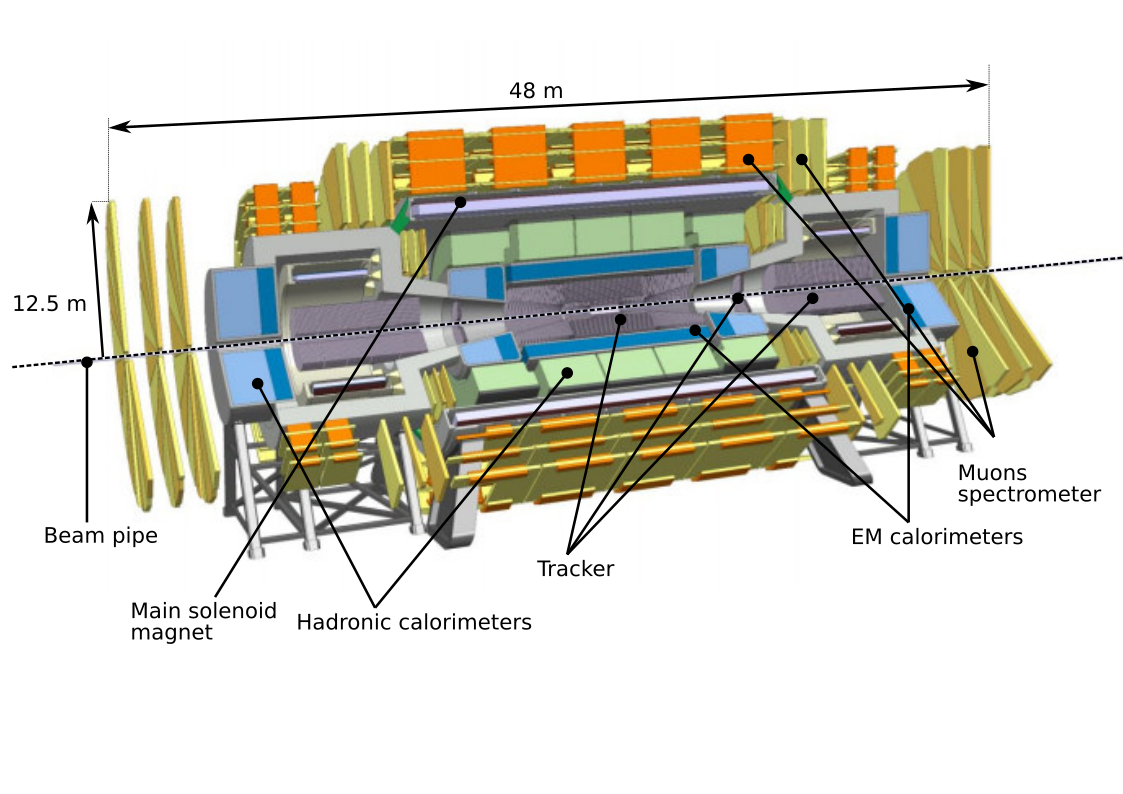
\includegraphics[trim={0 4cm 0.5cm 0},clip,width=\textwidth]{./Figures/FCCsvg1.png}
	\caption{FCC detector baseline concept.}
	\label{fig:FCC_detector}
\end{figure} 

%\begin{figure}
%	\centering
%	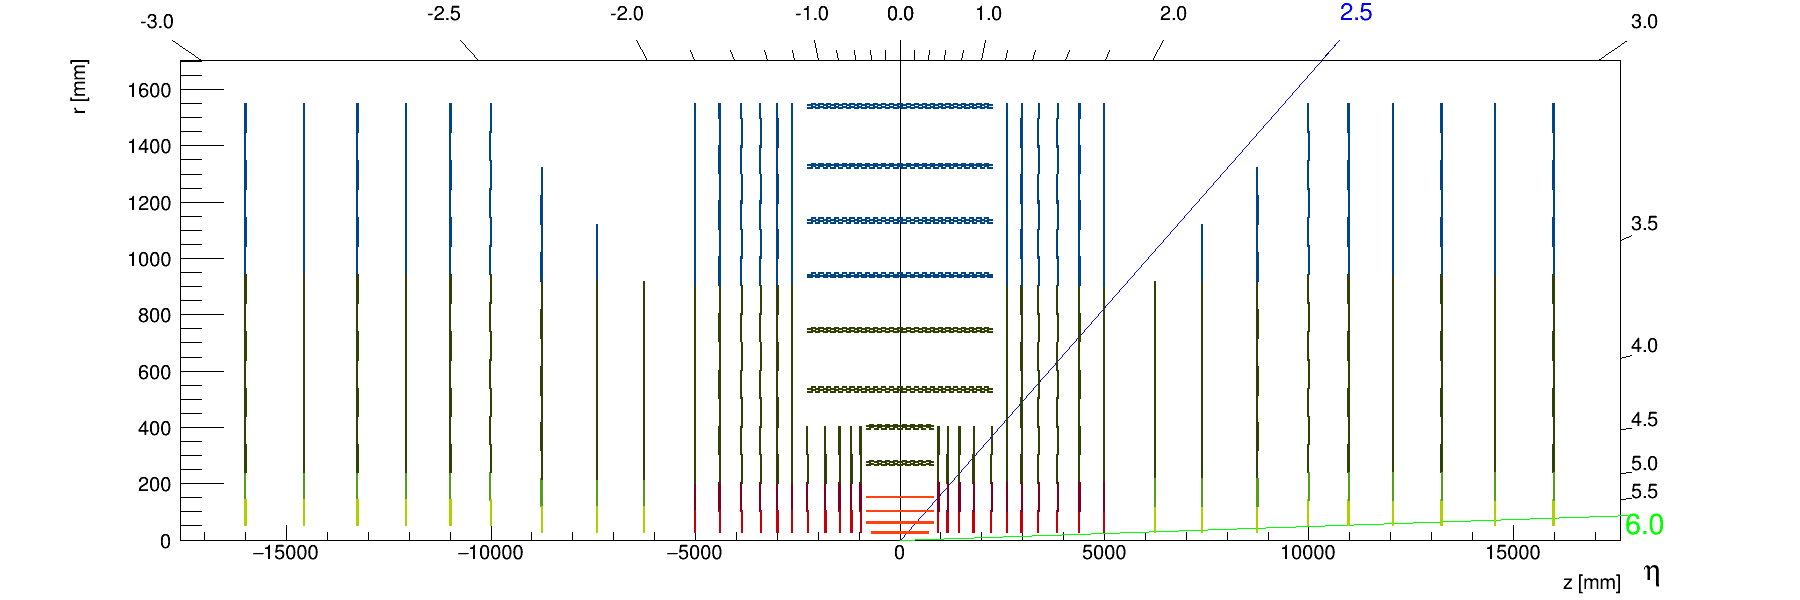
\includegraphics[trim={2cm 0 2cm 0},clip,width=\textwidth]{./Figures/FCC_tracker.png}
%	\caption{FCC detector proposed tracker layout.}
%	\label{fig:FCC_tracker}
%\end{figure} 

\subsection{FCC-hh physics program}

The FCC-hh physics program is vast and diverse. Within the SM, it includes the study of gauge bosons pair production and heavy flavor production, the measurement of the top quark's properties and the the study of the EWSB mechanism via multi-Higgs production. In addition, heavy ions collisions will allow for a deeper understanding of the Quark-Gluon Plasma. From a BSM standpoint, searches for supersymmetric and dark matter particles in new kinematic regimes can be pursued. A comprehensive review of the physics potential of the FCC-hh can be found here \cite{FCCyellow}. This document collects the results of the many studies that have been carried out since the beginning of the FCC initiative, in 2014.

Regarding Higgs pair production, a maximum precision on the SM cross section of $3\%$ is expected to be achieve using the $b\overline{b}\gamma\gamma$ final state. This would allow to constraint the Higgs triple coupling to be $\lambda_{hhh}\in [0.97,1.03]$. The $hh\rightarrow b\overline{b}b\overline{b}$ would allow for a $5\%$ precision on the SM cross section and to constraint the triple coupling to be $\lambda_{hhh}\in [0.9,1.5]$. In spite of the larger background yield, the $b\overline{b}b\overline{b}$ channel provides a reasonable number of events in the tail of the $m_{hh}$ distribution. As we discussed in section \ref{section:Higgs_pair}, the tail of this distribution does not have a large contribution from the triangle diagram. Therefore, the sensitivity to the Higgs triple coupling is expected to be smaller. However, the high energy regime can be more sensitive to new physics contributions which makes the $b\overline{b}b\overline{b}$ channel a very interesting one. 

The Higgs quartic coupling could be probed through triple Higgs production. In this case the most promising final state seems to be $b\overline{b}b\overline{b}\gamma\gamma$. This channel could constraint the Higgs quartic coupling to be $\lambda_{hhhh}\in [-4,16]$. % file "Thesis_Implementation.tex"
\clearpage

%%%%%%%%%%%%%%%%%%%%%%%%%%%%%%%%%%%%%%%%%%%%%%%%%%%%%%%%%%%%%%%%%%%%%%%%
%                                                                      %
%     File: Thesis_Background.tex                                      %
%     Tex Master: Thesis.tex                                           %
%                                                                      %
%     Author: Andre C. Marta                                           %
%     Last modified :  2 Jul 2015                                      %
%                                                                      %
%%%%%%%%%%%%%%%%%%%%%%%%%%%%%%%%%%%%%%%%%%%%%%%%%%%%%%%%%%%%%%%%%%%%%%%%

%%%%%%%%%%%%%%%%%%%%%%%%%%%%%%%%%%%%%%%%%%%%%%%%%%%%%%%%%%%%%%%%%%%%%%
\chapter{State of the art}
\label{chapter:state}

In this chapter we present the state of the art of searches for Higgs pairs production at the LHC and  feasibility studies targeting searches for this process at future colliders. In addition, previous studies focusing on the granularity of the hadronic calorimeter as a key detector parameter are also reviewed.

In section \ref{section:previous_searches}, we review the searches that have been conducted at the LHC by the ATLAS and CMS experiments. We include discussions on the different final states that were targeted and report on the constraints that were derived for the di-Higgs cross section and trilinear coupling. A brief overview of the current constraints on some BSM models is also presented. In section \ref{section:feasibility}, we present the results obtained from feasibility studies that access the discovery potential for this process at the HL-LHC and at the FCC-hh. In section \ref{sec:gran}, we present previous studies on the impact of the granularity of the hadronic calorimeter on the spatial resolution of hadrons and on the resolution of the jet mass and of jet substructure observables.

\section{Searches for Higgs pair production at the LHC}
\label{section:previous_searches}
%
%IDEAS FOR SECTION
%
%- Previous searches by ATLAS and CMS at the LHC \checkmark\\
%- Different decay channels used: pros and cons + compare achieved sensitivities \checkmark \\
%Channels: bbbb, bb tau tau, bb gamma gamma, gamma gamma WW, bb ZZ \checkmark \\
%- Models investigated and motivation \\
%- Exclusion limits

%The discovery of the Higgs boson is a strong evidence that the Higgs mechanism operates in Nature. However, by itself, it does not guarantee that the shape of the Higgs potential is the one depicted in figure \ref{fig:higgsV}, on the right. In order to reconstruct the Higgs potential and gain a deeper understanding of the mechanism that leads to the breaking of the electroweak symmetry one must measure the Higgs boson self-couplings, namely its three and four point interactions, whose strengths depend on the values of the parameters of the Higgs potential, as shown in section \ref{eq:higgs_couplings}.  
%
%However, in the SM, the cross section for the production of Higgs pairs through ggF is extremely small: $\sim30~$fb at the current CM energy achieved at the LHC (value computed at Next to Leading Order (NLO) accuracy) \cite{higgsCrossSection}. This value is approximately three orders of magnitude smaller than the production cross section of a single Higgs boson. In addition, this value has to be multiplied by the branching fraction of the chosen decay channel which further reduces the effective cross section of the full process. Nonetheless, ATLAS and CMS have conducted searches for this process whose results are summarized in this section.

The searches performed so far at the LHC by ATLAS and CMS covered different decay channels and targeted not only the SM process but also some BSM scenarios where di-Higgs production is enhanced. Neither could achieve enough statistical significance to declare the measurement of this process in the SM nor have found any significant deviation from the expected values. These searches resulted in upper limits for the cross section of di-higgs production in the SM and for the values of the parameters of BSM benchmark theories. From the limits on the cross section it is also possible to constraint the values of the Higgs self coupling, $k_{\lambda}=\lambda_{hhh}/\lambda_{hhh}^{SM}$.

The $hh\rightarrow b\overline{b}b\overline{b}$ channel \cite{hh2bbbbATLAS,hh2bbbbCMS} benefits from the large branching fraction of $h\rightarrow b\overline{b}$ ($\sim 58 \%$). In addition, ATLAS showed that this is the most sensitive channel to resonance masses over $500$ GeV \cite{hhATLAS}. However, this channel suffers with an overwhelming multijet background which drives the need for very tight trigger level cuts in order to bring the event rates down to manageable values.

The $hh\rightarrow b\overline{b}\tau\tau$ analysis \cite{hhbbtautau_CMS,ATLAShh2tautau} benefits from a sizable branching fraction of $h\rightarrow\tau^+\tau^-$ ($\sim 7.3\%$) and from a relatively small background contribution from other SM processes. These searches target the semi-leptonic decay of the $\tau\tau$ pair to reduce contamination from QCD processes.

The $hh\rightarrow b\overline{b}\gamma\gamma$ \cite{hhbbAA_CMS,hhAAbb_ATLAS},$WW^*\gamma\gamma$ \cite{hhATLAS,hhbbll_CMS}, $ZZ^*\gamma\gamma$ \cite{hhbbll_CMS} analysis can make use of very efficient diphoton triggers and isolation criteria that greatly reduce multijet background. In addition the excellent mass resolution of $h\rightarrow \gamma\gamma$ can be exploited. The $hh\rightarrow b\overline{b}WW^*$ channel also benefits from the large branching fraction of $h\rightarrow W^+W^-$ ($\sim 21 \%$).

%The most stringent upper limit on the cross section of Higgs pair production in the SM comes from the $hh\rightarrow b\overline{b}\gamma\gamma$ channel. The limit is $0.73$ pb at $95\%$ confidence level (CL) which is equivalent to $\sim$ 20 times the predicted SM cross-section. The Higgs boson self coupling is constrained at 95\% CL to be $-8.2<k_{\lambda}<13.3$. The analyzed data corresponds to an integrated luminosity of $19.7~\text{fb}^{-1}$ of proton-proton collisions at $\sqrt{s}=8$ TeV collected with the CMS detector. [REF]

The most stringent upper limit on the cross section of Higgs pair production comes from a combination of three searches using up to $36.1~\text{fb}^{-1}$ of proton-proton collision data at a CM energy of $\sqrt{s}=13$ TeV collected with the ATLAS detector \cite{ATLAShhComb}. The combination is based on the three most sensitive decay channels of Higgs boson pairs, i.e, $hh\rightarrow b\overline{b}\gamma\gamma$, $hh\rightarrow b\overline{b}\tau^+\tau^-$ and $hh\rightarrow b\overline{b}b\overline{b}$. The combined observed
limit on the non-resonant Higgs boson pair cross-section is $0.223$ pb at $95\%$ CL,
which corresponds to $6.7$ times the cross-section predicted by the SM. The ratio of the Higgs boson self-coupling to its SM expectation, $k_{\lambda}$, is constrained, at $95\%$ CL, to be $-5.0<k_{\lambda}<12.1$.

The upper limits on the cross section (at $95$\% CL) of Higgs pair production at $8$ TeV as a function of the mass of a spin 0 resonance are summarized in figure \ref{fig:ATLAS_CMS_BSMlim}(a) \cite{hhbbAA_CMS}. The limits were obtained using data collected with the CMS detector and come from searches using different final states, namely, $b\overline{b}\gamma\gamma$ (blue), $b\overline{b}b\overline{b}$ (red and pink) and $b\overline{b}\tau\tau$ (green). Depending on the analysis, the corresponding integrated luminosity varies between $17.9~\text{fb}^{-1}$ and $19.7~\text{fb}^{-1}$. The results are usually interpreted in the framework of the Randall-Sundrum models such that the spin 0 resonance corresponds to the radion that decays to a pair of Higgs bosons. For a mass of $1$ TeV the upper limit on the cross section is approximately $12$ pb.

The upper limits on the cross section (at $95\%$ CL) of Higgs pair production as a function of the mass of a heavy scalar Higgs, $m_H$, are summarized in figure \ref{fig:ATLAS_CMS_BSMlim}(b) \cite{ATLAShhBSMcomb}. The limits were obtained through a combination of searches performed in the $hh\rightarrow b\overline{b}\gamma\gamma$, $hh\rightarrow b\overline{b}b\overline{b}$, $hh\rightarrow b\overline{b}\tau^+\tau^-$ and $hh\rightarrow \gamma\gamma WW^*$ channels using proton-proton collision data corresponding to an integrated luminosity of $20.3~\text{fb}^{-1}$ collected with the ATLAS detector at a CM energy of $\sqrt{s}=8$ TeV. The improvement above $m_H=500$ GeV is due to the sensitivty of th $hh\rightarrow b\overline{b}b\overline{b}$ analysis. For $m_H=900$ GeV the observed limit is $0.015$ pb.

%\begin{figure}
%	\centering
%	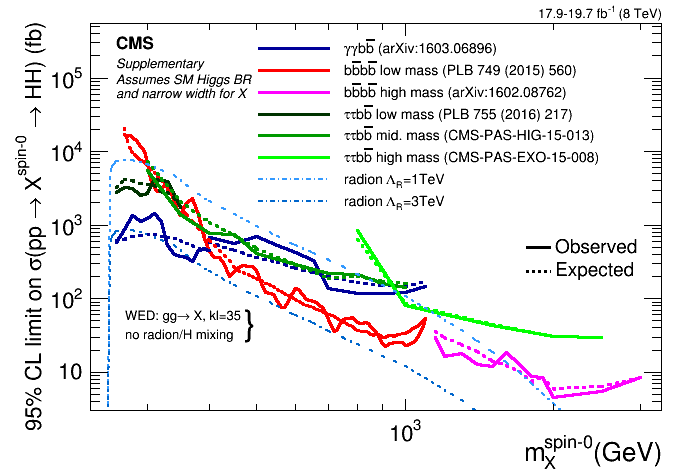
\includegraphics[width=.7\textwidth]{./Figures/CMS_spin0_exc.png}
%	\label{fig:CMS_BSMlim}
%	\caption{Exclusion limits on the mass of a spin 0 resonance from searches for Higgs pair production with the CMS detector.}
%\end{figure}

\begin{figure}
	\centering
	\begin{minipage}{.5\textwidth}
		\centering
		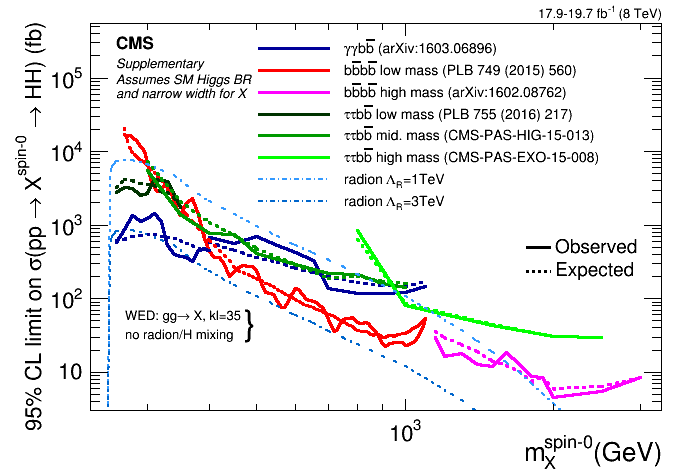
\includegraphics[width=\linewidth]{./Figures/CMS_spin0_exc.png}
	\end{minipage}%
	\begin{minipage}{.5\textwidth}
		\centering
		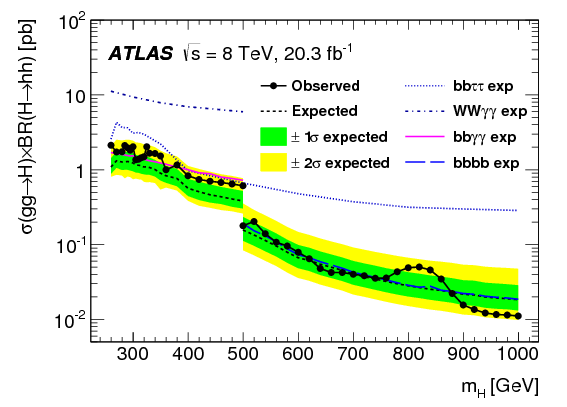
\includegraphics[width=\linewidth]{./Figures/ATLASmH.png}
	\end{minipage}
	\begin{minipage}[t]{0.5\textwidth}
		\caption*{(a)}
		%\label{fig1}
	\end{minipage}%%%
	\hfill
	\begin{minipage}[t]{0.5\textwidth}
		\caption*{(b)}
		%\label{fig2}
	\end{minipage}
	\caption{Exclusion limits (at $95\%$ CL) on the cross section of resonant Higgs pair production from the decay of heavy scalar particles. These results were obtained using proton-proton collision data collected with the CMS (a) and ATLAS (b) detector at a CM energy of $\sqrt{s}=8$ TeV and result from the combination of different channels. Plots from Refs. \cite{hhbbAA_CMS, ATLAShhBSMcomb}, respectively.}
	\label{fig:ATLAS_CMS_BSMlim}
\end{figure}

\section{Feasibility studies for high-luminosity and future colliders}
\label{section:feasibility}

%IDEAS FOR SECTION \\
%- HL-LHC feasibility study \cite{hhFeasibility},\cite{hhFeasibility_LHC},\cite{hhFeasibility1_LHC} \\
%- FCC hh to 4b (Selvaggi et al.)  \cite{hh+jet_100TeV}, \cite{hhFeasibility1_100TeV}\\

Without any BSM contribution, the discovery of Higgs pairs production in the four b quarks final state at the LHC is highly unlikely even considering the total expected integrated luminosity of $300~\text{fb}^{-1}$. There might be evidence for this process but retrieving useful information about the value of the Higgs trilinear coupling will remain out of reach. Nonetheless, the HL-LHC as well as future colliders pose a good opportunity for the discovery and precision studies of this process. Therefore, Monte Carlo studies assessing the feasibility of searches for $hh\rightarrow b\overline{b}b\overline{b}$ at the HL-LHC and at the FCC-hh have been performed.

For the HL-LHC, a study including the $pp\rightarrow b\overline{b}b\overline{b}$, $pp\rightarrow b\overline{b}jj$, $pp\rightarrow jjjj$ and $pp\rightarrow t\overline{t}\rightarrow b\overline{b}jjjj$ backgrounds reports a significance ($S/\sqrt{B}$) of $4$ ($1.3$) for an integrated luminosity of $3000~(300)~\text{fb}^{-1}$ \cite{hhFeasibility}. The analysis is performed in three orthogonal regions (boosted, intermediate and resolved) and the reported significance is obtained from the combination of these three regions. The highest significance ($S/\sqrt{B}=2.9$) is achieved in the boosted category. In addition, the impact of pile up is evaluated. Considering a mean pile up of $80$ and making use of jet grooming techniques, a significance of $3.1$ ($1.0$) for an integrated luminosity of $3000~(300)~\text{fb}^{-1}$ is reported (also considering the three analysis regions). This work makes use of artificial neural networks (ANN's) as well as of jet substructure observables to further increase the signal-background separation. Furthermore, single Higgs backgrounds, namely $Z(\rightarrow b\overline{b})h(\rightarrow b\overline{b})$, $t\overline{t}h(\rightarrow b\overline{b})$ and $b\overline{b}h(\rightarrow b\overline{b})$, are shown to be negligible for the analysis, when compared to the dominant QCD multijet background.

ATLAS and CMS also carried out preliminary studies for the sensitivity on the trilinear coupling at the HL-LHC. Several channels have been investigated: $hh\rightarrow  b\overline{b}\gamma\gamma$, $hh\rightarrow b\overline{b} \tau^+ \tau^-$, $hh\rightarrow b\overline{b} WW^*$ and $hh\rightarrow  b\overline{b}b\overline{b}$. The $b\overline{b}\gamma\gamma$ final state is the most sensitive one. In this channel, ATLAS and CMS reported significances of $1.05\sigma$ \cite{ATLAShh2bbAA_HL} and $1.6\sigma$ \cite{CMShh2bbAA_HL}, respectively, for an integrated luminosity of $3000~\text{fb}^{-1}$. Taking, as an example, the ATLAS result, the achieved significance translates to an upper limit on the total di-Higgs cross section of approximately twice the SM value. This corresponds to an exclusion limit of $-0.8<k_{\lambda}<7.7$. The analysis conducted by ATLAS in this channel is done at generator level. The energy and momenta of the particles are smeared to simulate the detector's response. A mean pile up of $200$ is considered. No MVA techniques are employed in the analysis. 

For the $hh\rightarrow  b\overline{b}b\overline{b}$ channel, ATLAS states that a cross section $5.2$ times larger than the SM value can be excluded at $95\%$ CL, with systematic uncertainties being taken into consideration. The Higgs trilinear coupling is expected to be constrained to $-3.5<k_{\lambda}<11$. These results are based on the extrapolation of the current results obtained with the 2016 dataset, comprising an integrated luminosity of $10.1~\text{fb}^{-1}$. This study is based only on the resolved analysis documented in Ref. \cite{hh2bbbbATLAS}.

For the FCC-hh, a recent study that uses as signal sample $pp\rightarrow hhj\rightarrow b\overline{b}b\overline{b}j$ and that includes only the irreducible background $pp\rightarrow b\overline{b}b\overline{b}j$ reports a significance of $6.61$ for an integrated luminosity of $30~\text{ab}^{-1}$, considering an analysis that targets the boosted region \cite{hh+jet_100TeV}. The extra jet in the signal sample has $p_T>200$ GeV which provides the Higgs pair with a large Lorentz boost. This enhances the sensitivity to the Higgs boson self coupling because it favors highly boosted virtual Higgs bosons decaying to a pair of Higgs bosons. The analysis relies on the jet substructure observable $\tau_{21}$ and on a tight mass cut around the Higgs mass. No multivariate techniques are employed. 

A study comparing the feasibility of the search for di-Higgs production in the $b\overline{b}b\overline{b}$ in the HL-LHC and at the FCC-hh was presented in Ref. \cite{hhFeasibility1_100TeV}. Only the irreducible background is considered. For a boosted region, cut based analysis, a significance of $1.1$ is reported for an integrated luminosity of $3~\text{ab}^{-1}$ at $\sqrt{s}=14$ TeV (HL-LHC). For an integrated luminosity of $10~\text{ab}^{-1}$ at $\sqrt{s}=100$ TeV, which corresponds to the FCC-hh, this number is $5.7$. While the significance is large for the FCC-hh, the reported signal to background ratio ($S/B$) is approximately one order of magnitude smaller, which means the measurement might be more sensitive to systematic uncertainties on the backgrounds. 

\section{Hadronic calorimeter granularity studies}
\label{sec:gran}

Even before the baseline design for the FCC-hh was established, there were studies regarding the impact of the granularity of the calorimeters in the spatial resolving power of hadronic showers and on the resolution of jet mass and substructure variables. These studies targeted the development of future colliders and greatly influenced the baseline design of the FCC-hh.

The granularity of hadronic calorimeters is a key parameter for future collider detectors because it determines how well we can resolve energy deposits from pileup vertices and highly-boosted jet topologies. In Ref. \cite{FCC_HCALgran_doubleK}, the use of smaller calorimeter cells (smaller than the ones that are used in currently operating hadronic calorimeters) to resolve individual hadrons is investigated. 
\begin{figure}
	\centering
	\begin{minipage}{.5\textwidth}
		\centering
		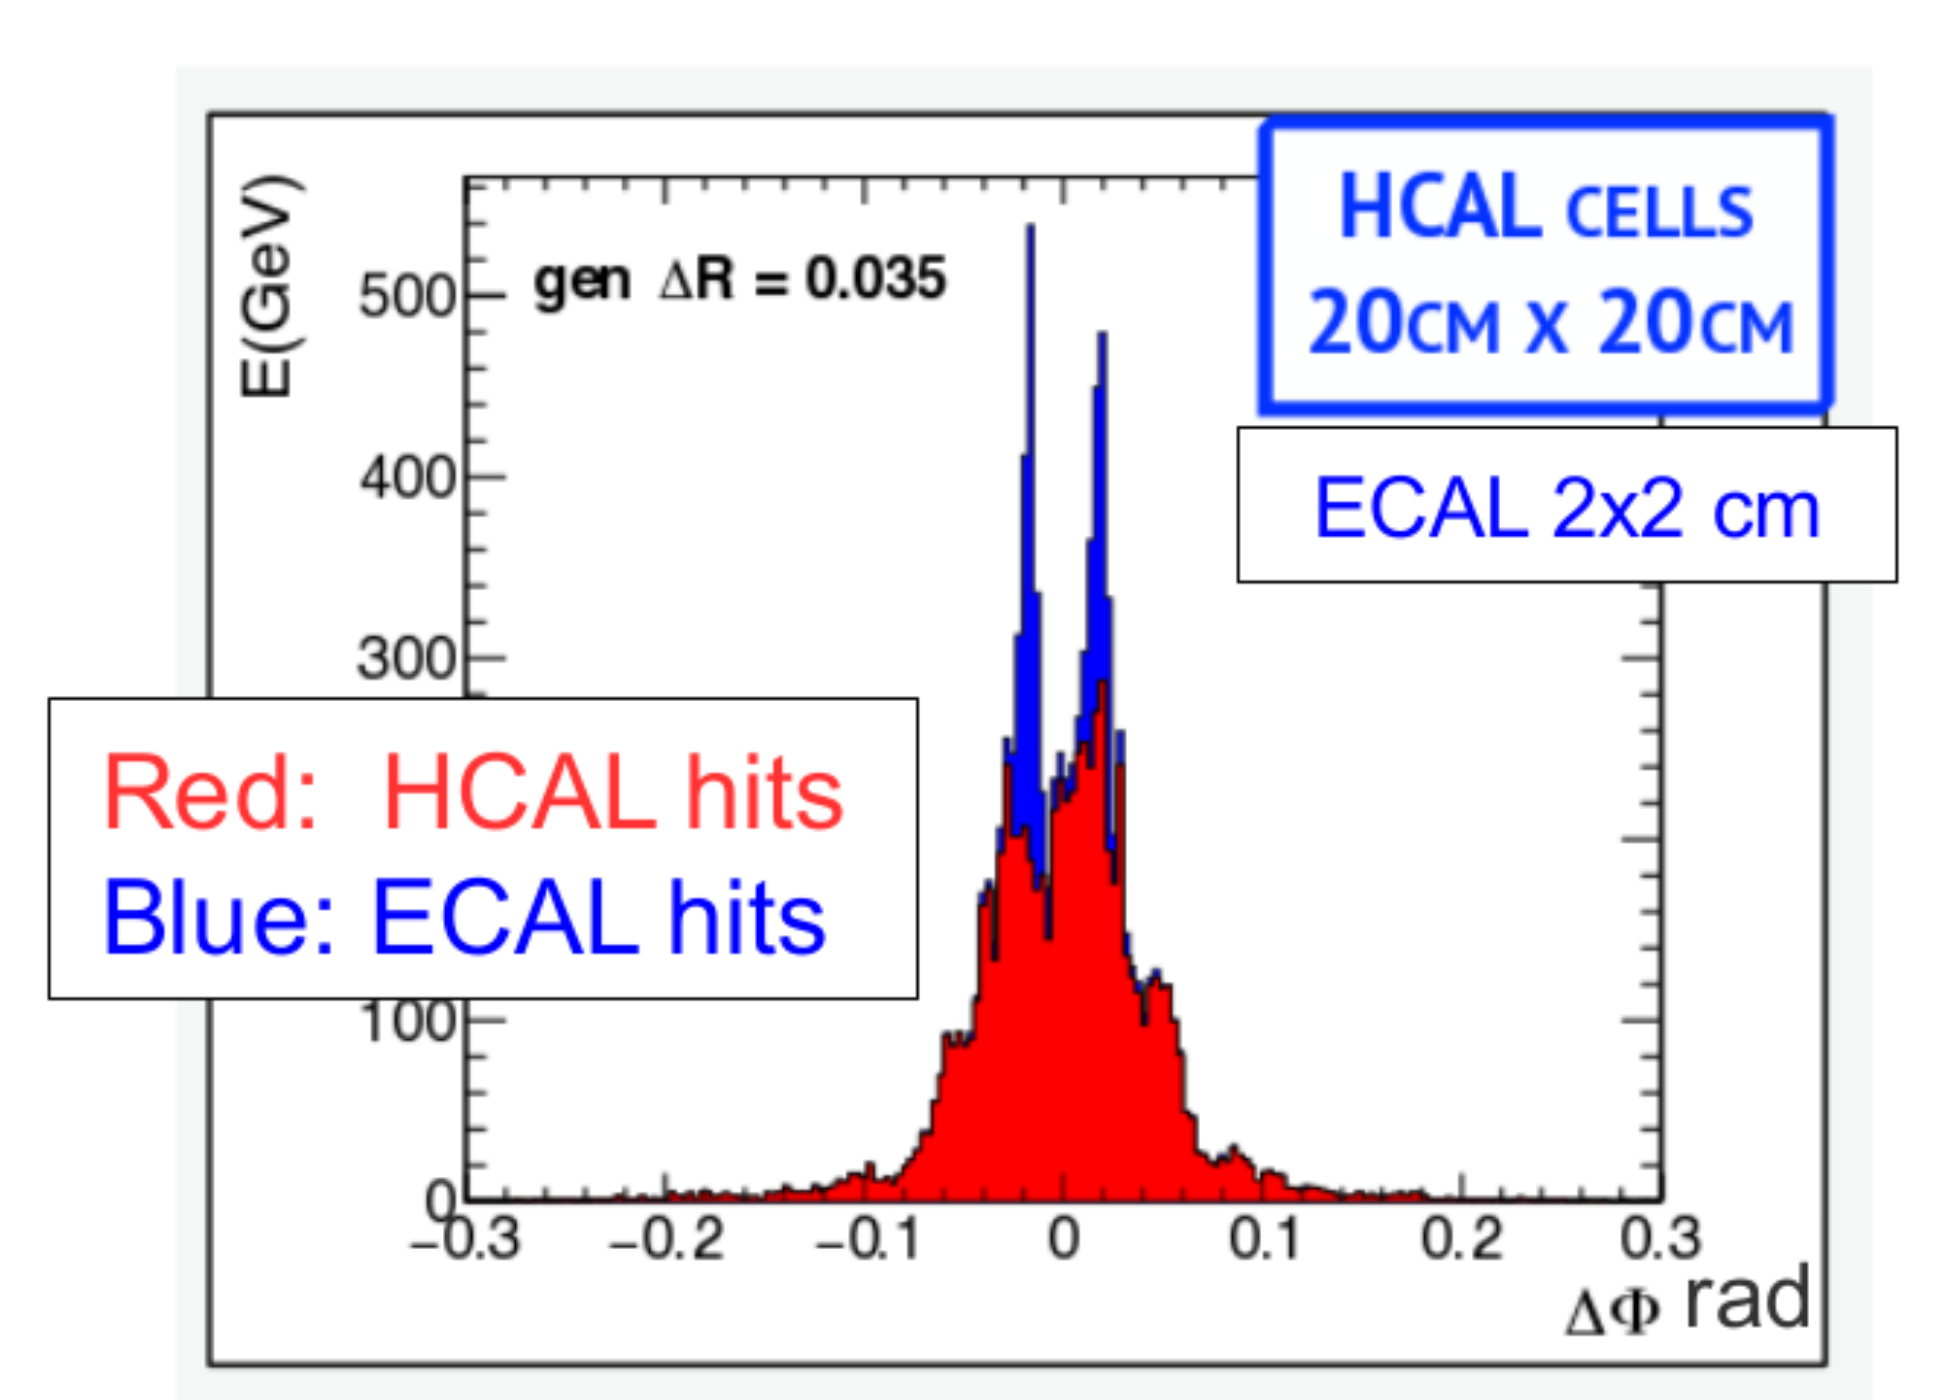
\includegraphics[trim={0 0 0 .4cm},clip,width=\linewidth]{./Figures/hcal_gran_doubleK1.png}
	\end{minipage}%
	\begin{minipage}{.5\textwidth}
		\centering
		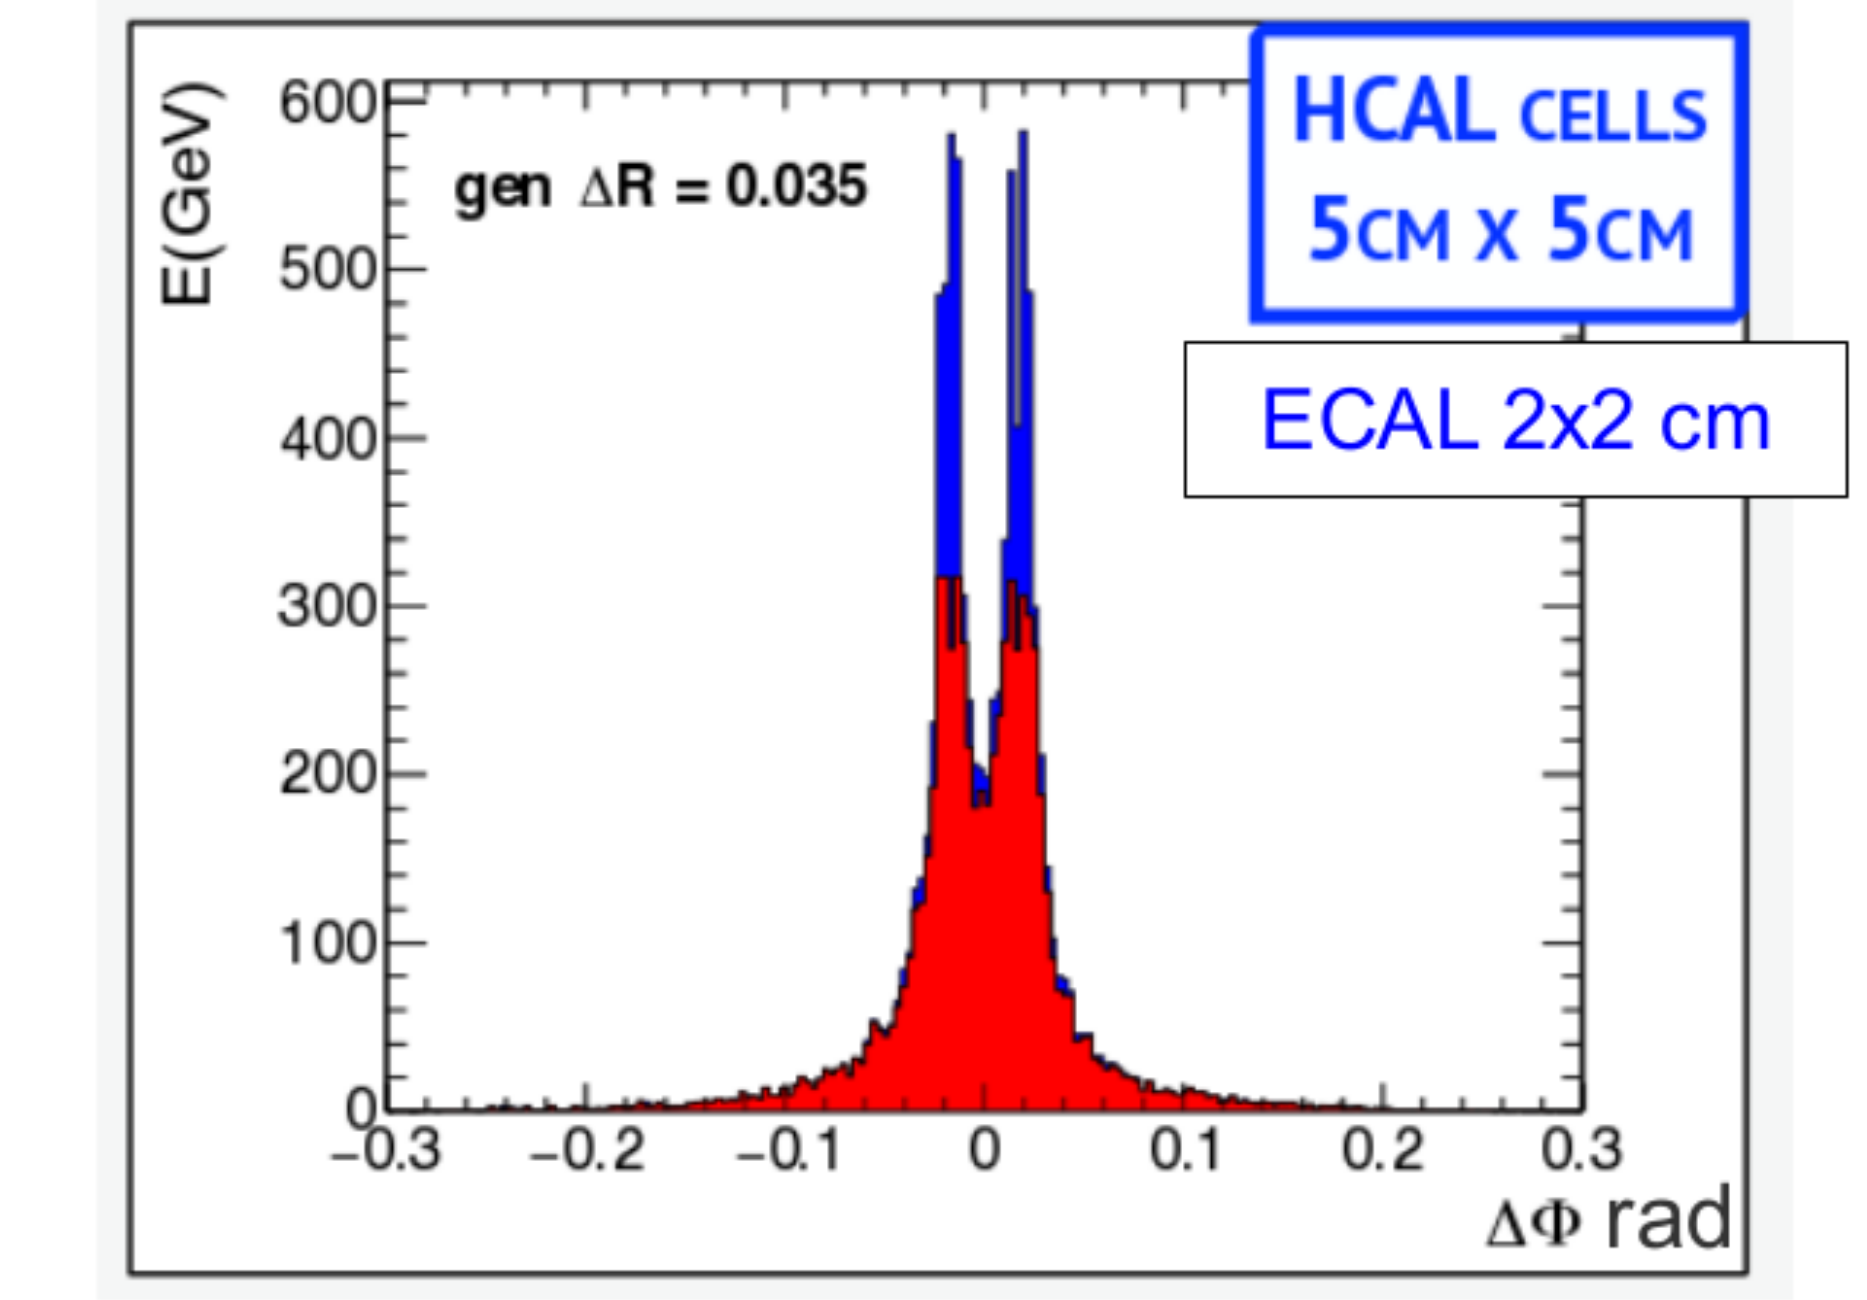
\includegraphics[width=\linewidth]{./Figures/hcal_gran_doubleK2.png}
	\end{minipage}
	\begin{minipage}[t]{0.5\textwidth}
		\caption*{(a)}
		%\label{fig1}
	\end{minipage}%%%
	\hfill
	\begin{minipage}[t]{0.5\textwidth}
		\caption*{(b)}
		%\label{fig2}
	\end{minipage}
	\caption{Azimuthal distribution of the energy deposits in the ECAL and HCAL for a pair of $K_L^0$ with $E=100$ GeV for an hadronic calorimeter with $20~\text{cm}\times 20~\text{cm}$ (a) and $5~\text{cm}\times 5~\text{cm}$ (b). Figures from Ref. \cite{BOOST2017} (based on Ref. \cite{FCC_HCALgran_doubleK}).}
	\label{fig:hcal_gran_doubleK}
\end{figure}
For two Kaons ($K_L^0$) with an energy of $100$ GeV each and with a truth level separation ($\Delta R$) equal to $0.035$ the energy deposited in the ECAL (blue) and HCAL (red) is shown as a function of $\Delta R$ for HCAL cells with sizes $20~\text{cm}\times 20~\text{cm}$ ($\Delta \eta\times \Delta\phi=0.1\times 0.1$) and $5~\text{cm}\times 5~\text{cm}$ ($\Delta \eta\times \Delta\phi=0.022\times 0.022$) in figures \ref{fig:hcal_gran_doubleK}(a) and \ref{fig:hcal_gran_doubleK}(b), respectively. The ECAL segmentation is equal to $2~\text{cm}\times 2~\text{cm}$. It is shown that for a granularity of $\Delta \eta\times \Delta\phi=0.022\times 0.022$ both hadrons can be resolved in the HCAL.

Additional studies focusing on the jet mass resolution and on the resolution of jet substructure observables were performed for three calorimeter configurations (HCAL and ECAL). Some of these studies were presented in major conferences focused on future colliders, namely FCC week 2015 and 2016 and BOOST 2017. Here, we show results presented in Refs. \cite{FCCweek2015,FCCweek2016,BOOST2017}. The calorimeter configurations tested are: HCAL(ECAL) $0.1(0.025)~\eta \times 5.6(1.4)~^{\circ}~\phi$, HCAL(ECAL) $0.05(0.012)~\eta \times 2.8(0.7)~^{\circ}~\phi$ and HCAL(ECAL) $0.025(0.006)~\eta \times 1.4(0.35)~^{\circ}~\phi$. For the segmentation in $\phi$ the numbers are give in degrees. For the HCAL, these correspond to approximately $\Delta\eta\times\Delta\phi=0.1\times0.1,0.05\times 0.05, 0.025\times0.025$. 

For $t\overline{t}$ events generated at NLO with MadGraph5 and passed through Delphes 3.2 to simulate detector response, the energy flow jet mass distribution for $p_T(\text{jet})>3$ TeV is shown in figure \ref{fig:hcal_gran_jet_mass}(a) \cite{FCCweek2015}. The jet mass resolution is shown in figure \ref{fig:hcal_gran_jet_mass}(b). For $\Delta\eta\times\Delta\phi=0.1\times0.1$ cells the root mean square (RMS) of the distribution is $0.130$. This value decreases to $0.090$ and $0.088$ for $\Delta\eta\times\Delta\phi=0.05\times0.05$ and $\Delta\eta\times\Delta\phi=0.025\times0.025$ cells, respectively. This indicates that the mass resolution increases as the granularity of the HCAL increases.

Regarding jet substructure, the resolution of the $\tau_{32}$ variable in QCD dijet events generated with Pythia8 is shown in figure \ref{fig:hcal_gran_tau32}(a) for particle flow jets \cite{FCCweek2015}. The same distribution is shown in figure \ref{fig:hcal_gran_tau32}(b) for calorimeter jets. Regardless of the type of jets used (eflow or tower jets), the $\tau_{32}$ resolution increases as the HCAL resolution increases. In addition, it is important to note that the resolution is a lot worse when using tower jets which is an indication that exploiting tracking information is vital to achieve a good resolution in substructure variables. 

Another interesting result, presented in Ref. \cite{BOOST2017}, has to do with the overlap between the $\tau_{21}$ distribution for jets resulting from QCD interactions and from the decay of a $W$ boson. Jets with $p_T$ of $2.5$ TeV show a reduction in overlap ($80\%\rightarrow 60\%$) going from $\Delta\eta\times\Delta\phi=0.1\times 0.1$ to $\Delta\eta\times\Delta\phi=0.005\times 0.005$ HCAL cells. For $5(10)$ TeV jets the overlap varies from $88(91)\%$ to $78(85)\%$. However, for $20$ TeV jets, the change in the HCAL granularity does not significantly modify the overlap, as is shown in figure \ref{fig:overlap}. 

In summary, previous studies focus on the impact of granularity in the resolution of jet mass and jet substructure observables. We did not find any studies that explored the change in the significance of a given analysis as a function of the granularity or of the detector configuration.

\begin{figure}
	\centering
	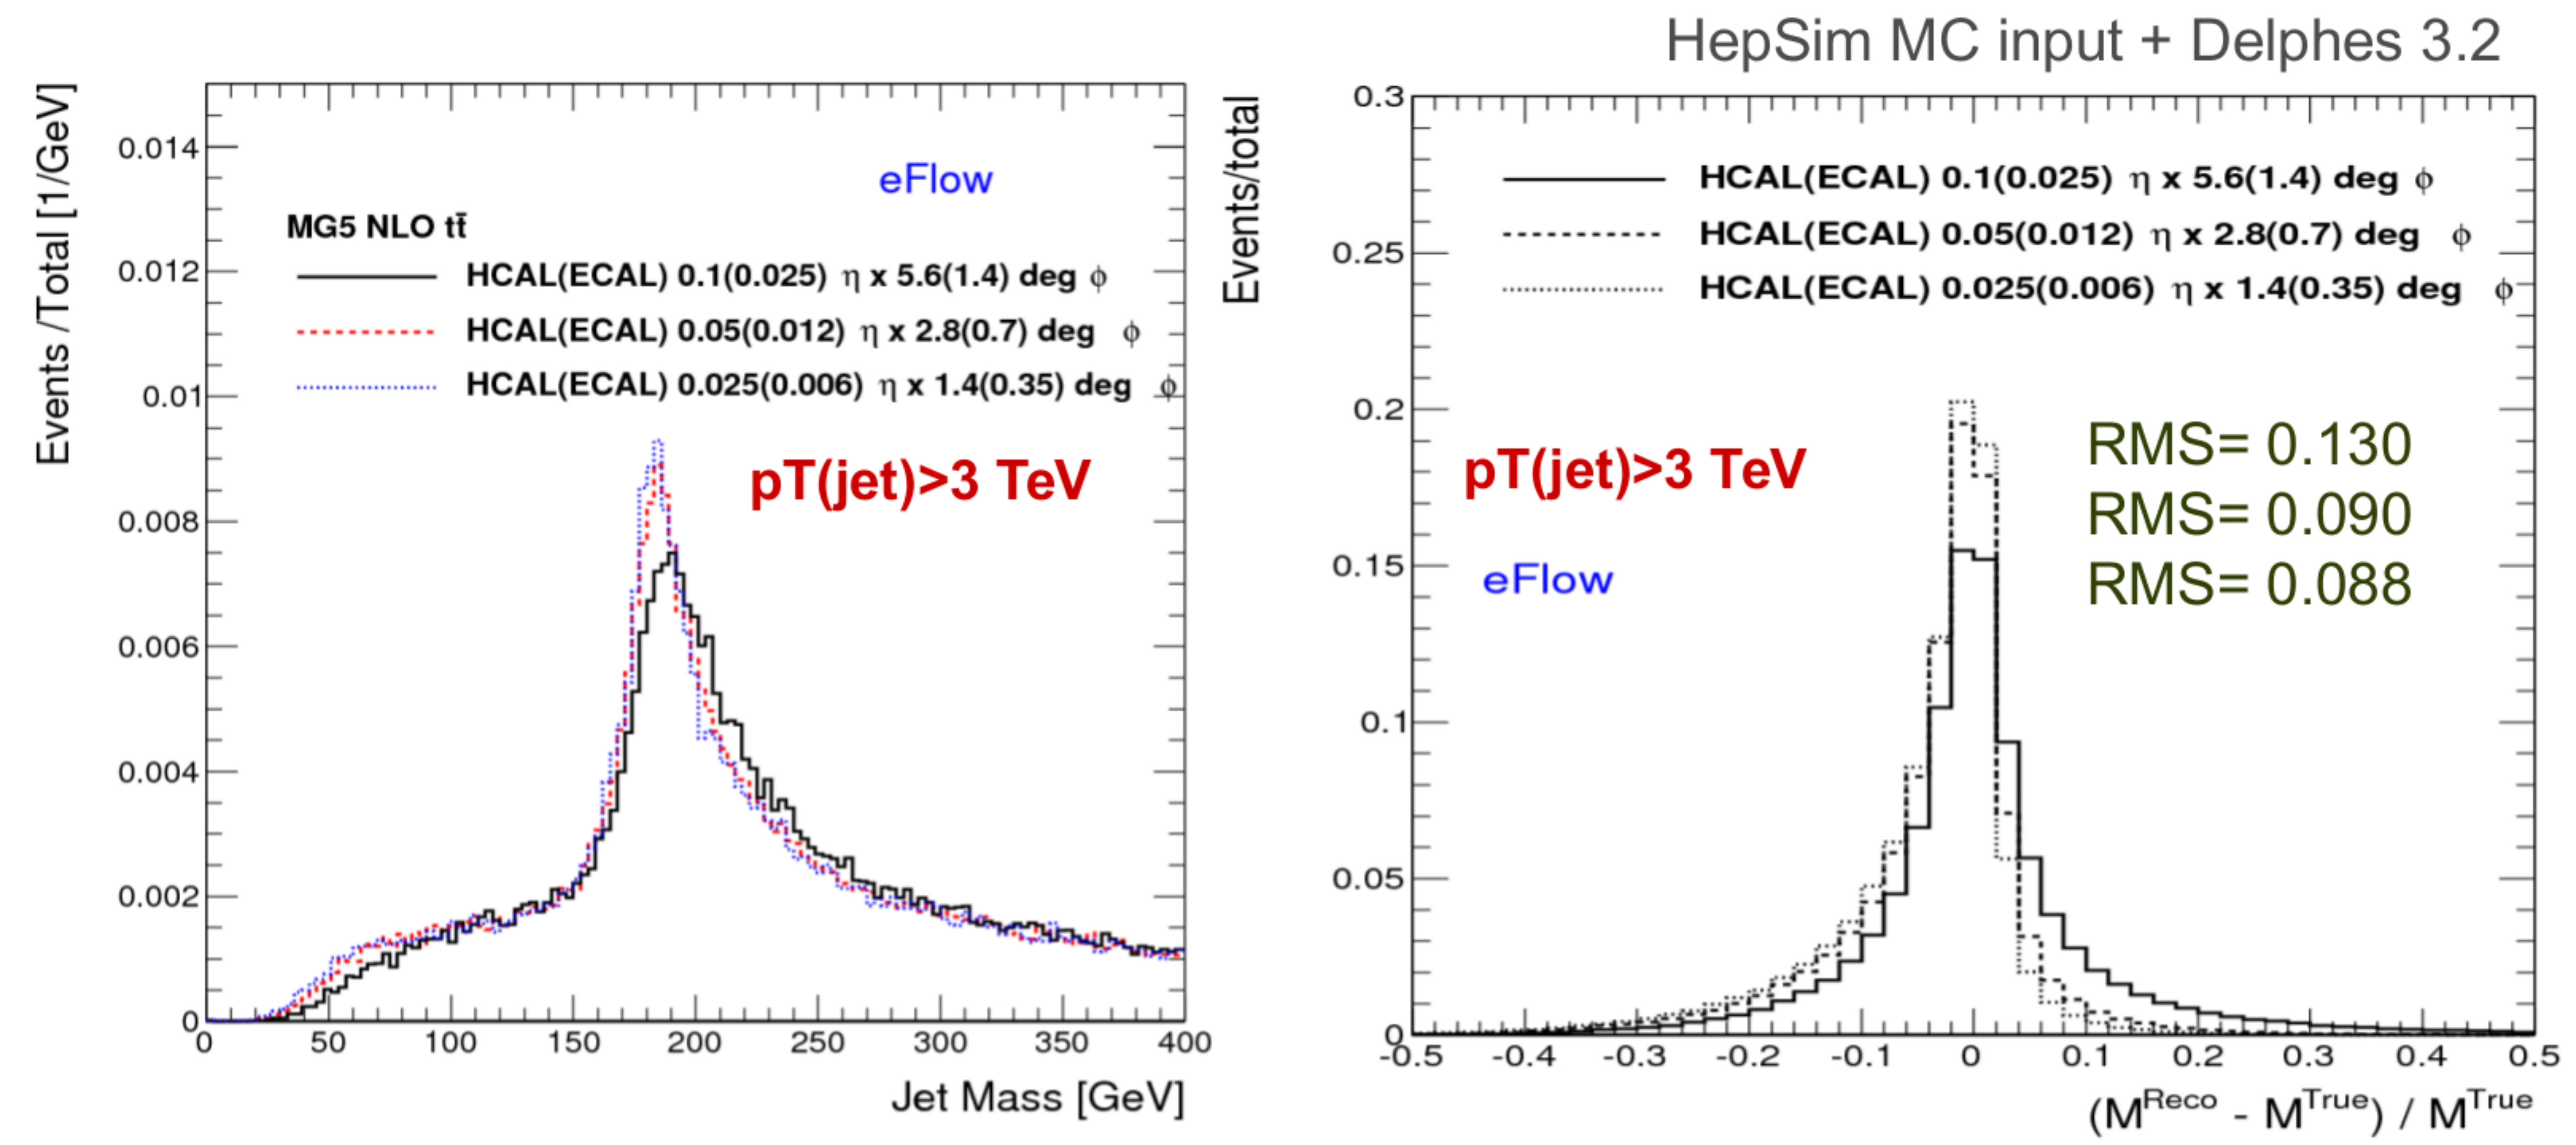
\includegraphics[width=0.9\textwidth]{./Figures/hcal_gran_jet_mass.png}
	\begin{minipage}[t]{0.45\textwidth}
		\caption*{(a)}
		%\label{fig1}
	\end{minipage}%%%
	\hfill
	\begin{minipage}[t]{0.45\textwidth}
		\caption*{(b)}
		%\label{fig2}
	\end{minipage}
	\caption{Jet mass (a) and jet mass resolution (b) plots in $t\overline{t}$ events for eflow jets with $p_T>3$ TeV for three different HCAL and ECAL configurations: HCAL(ECAL) $0.1(0.025)~\eta \times 5.6(1.4)~^{\circ}~\phi$, HCAL(ECAL) $0.05(0.012)~\eta \times 2.8(0.7)~^{\circ}~\phi$ and HCAL(ECAL) $0.025(0.006)~\eta \times 1.4(0.35)~^{\circ}~\phi$. Plots from Ref. \cite{BOOST2017}.}
	\label{fig:hcal_gran_jet_mass}
\end{figure}

\begin{figure}
	\centering
	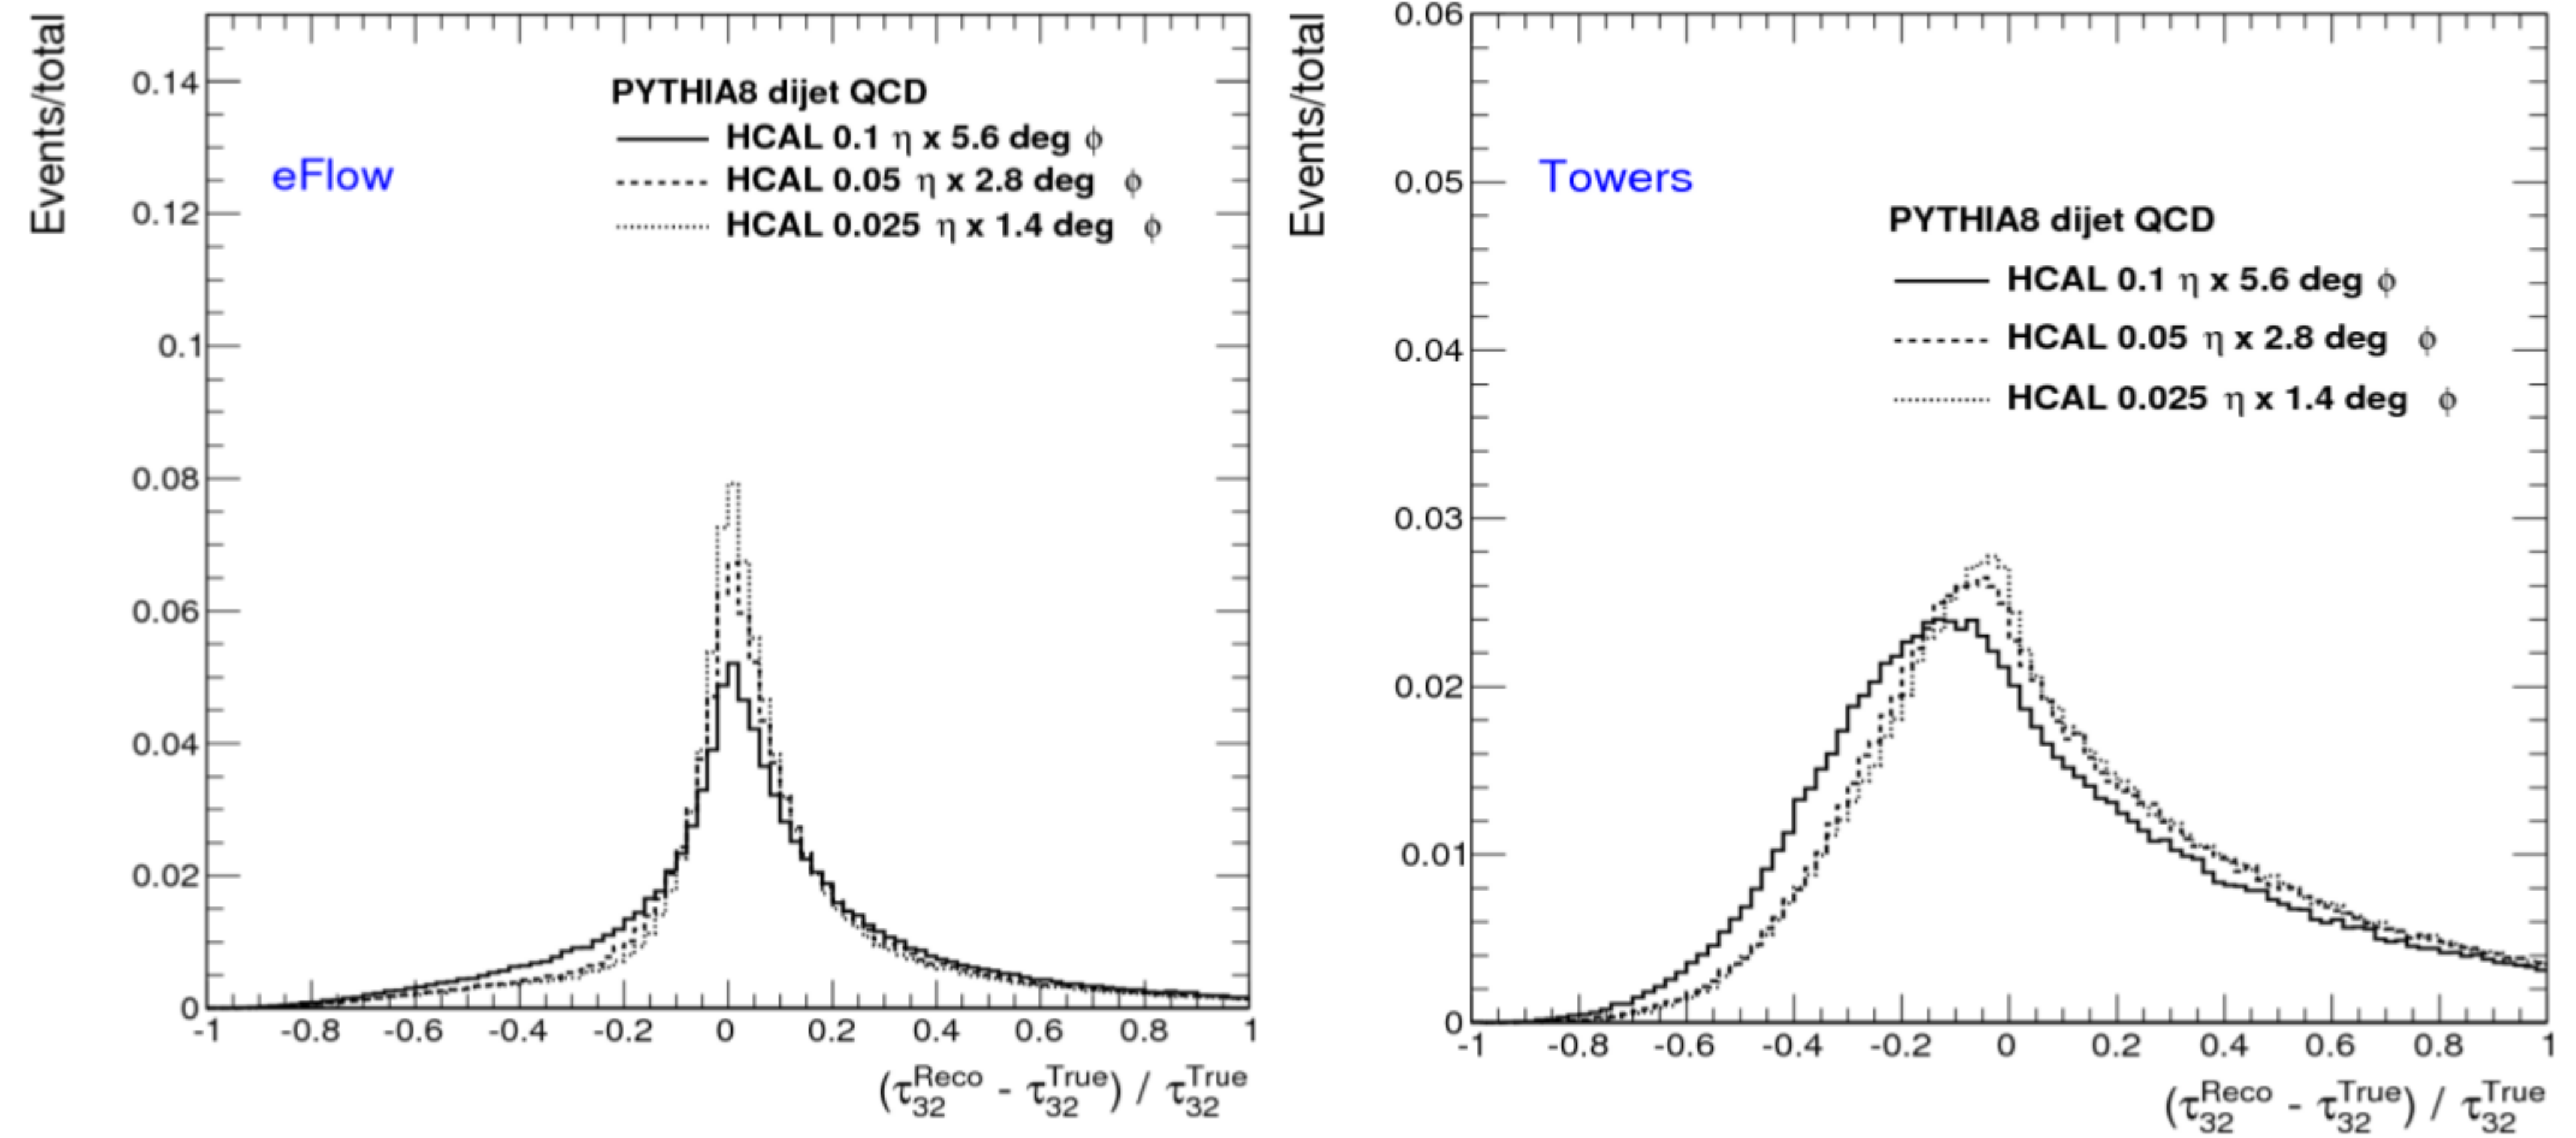
\includegraphics[width=0.9\textwidth]{./Figures/hcal_gran_tau32.png}
	\begin{minipage}[t]{0.45\textwidth}
		\caption*{(a)}
		%\label{fig1}
	\end{minipage}%%%
	\hfill
	\begin{minipage}[t]{0.45\textwidth}
		\caption*{(b)}
		%\label{fig2}
	\end{minipage}
	\caption{$\tau_{32}$ resolution plots for QCD dijet events reconstructed using eflow jets (a) and tower jets (b). Plots from Ref. \cite{FCCweek2015}.}
	\label{fig:hcal_gran_tau32}
\end{figure}

\begin{figure}
	\centering
	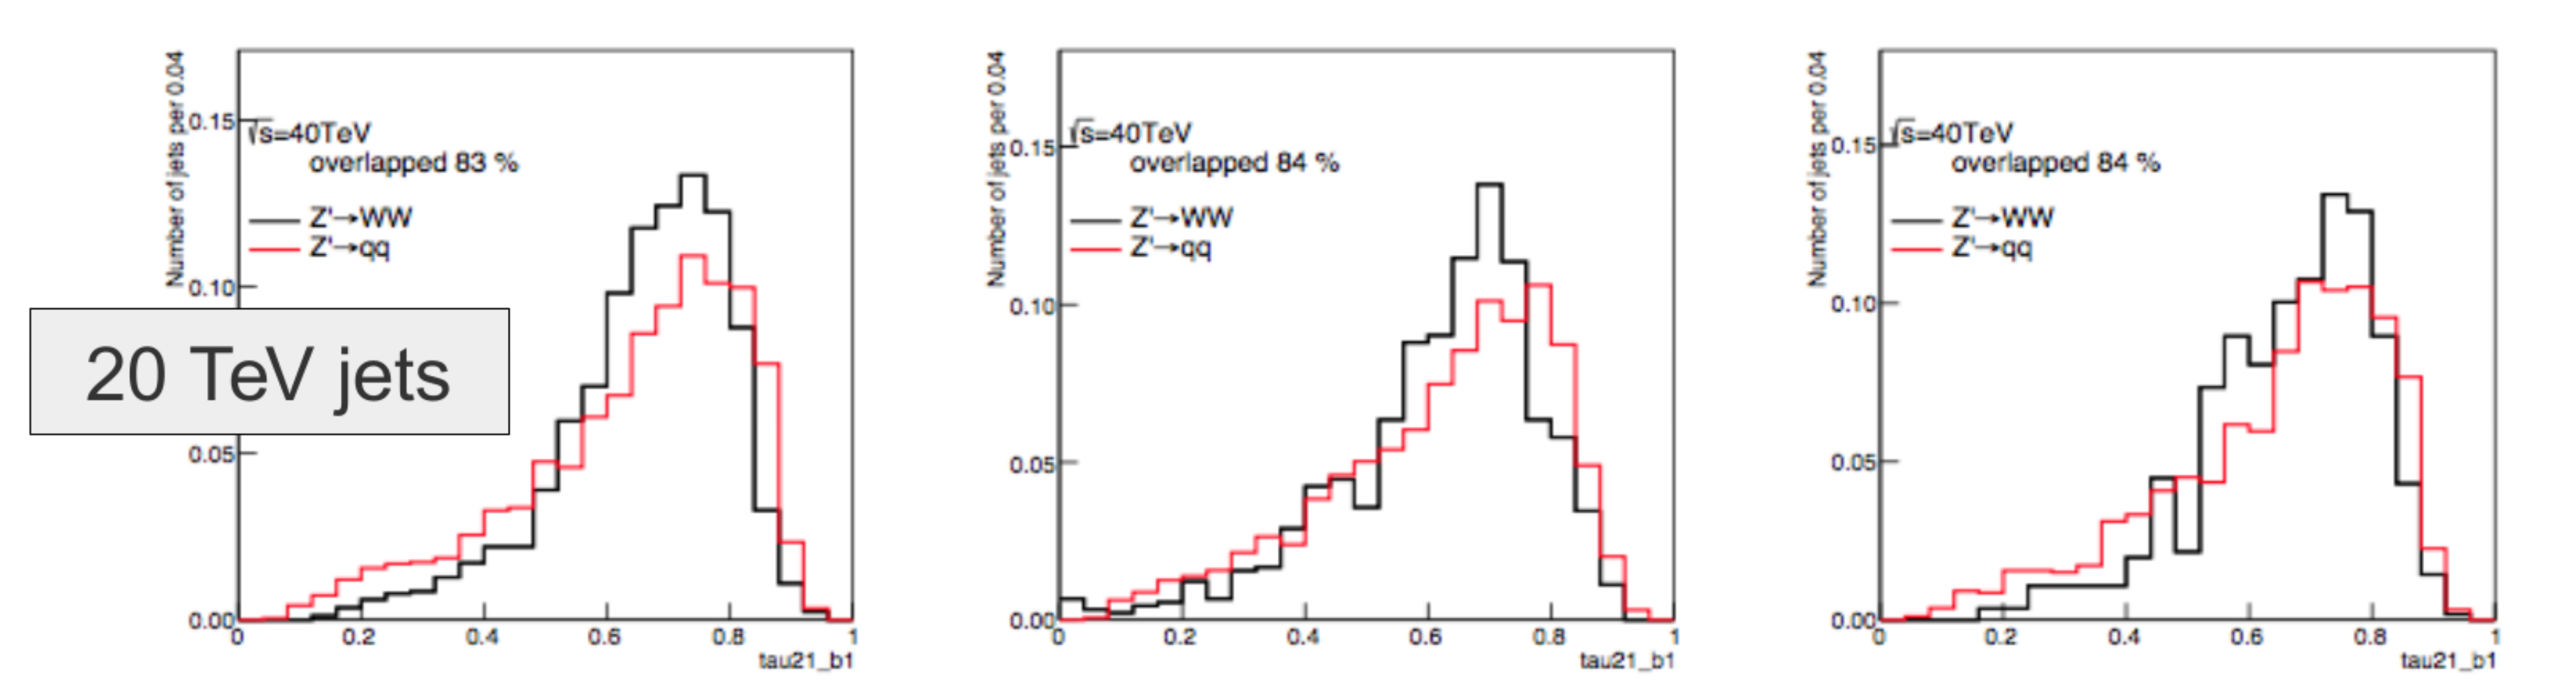
\includegraphics[width=0.9\textwidth]{./Figures/overlap.png}
	\caption{$\tau_{21}$ variable for $20$ TeV $W$ (black) and QCD jets (red) for three HCAL granularities: $\Delta\eta\times\Delta\phi=0.1\times 0.1$ (left), $\Delta\eta\times\Delta\phi=0.022\times 0.022$ (middle) and $\Delta\eta\times\Delta\phi=0.005\times 0.005$ (right). Plots from Ref. \cite{BOOST2017}.}
	\label{fig:overlap}
\end{figure}

%?? 
%IDEAS FOR SECTION\\
%- Introduce machine learning as a state of the art computational techinque very often used nowadays in physics analysis \\
%- Examples: analysis (refer back to studies presented in previous section since they both use MVAs), b tagging algorithms \\
%- Packages used: sklearn, TMVA (ROOT)\\
%- Discuss in some detail a BDT if we use it in the analysis \\
%------------------------------------------------------------------\\
%
%Machine learning techniques such as neural networks and boosted decision trees are widely used today in high energy physics. These state of the art computational techniques have proven to be useful and reliable tools to further increase the signal-background separation with respect to the traditional cut-based analysis. 
%
%Two examples of analysis employing MVA methods are the ones described in the previous section. 

 % add new .tex files for new chapters
\clearpage

%%%%%%%%%%%%%%%%%%%%%%%%%%%%%%%%%%%%%%%%%%%%%%%%%%%%%%%%%%%%%%%%%%%%%%%%
%                                                                      %
%     File: Thesis_Results.tex                                         %
%     Tex Master: Thesis.tex                                           %
%                                                                      %
%     Author: Andre C. Marta                                           %
%     Last modified :  2 Jul 2015                                      %
%                                                                      %
%%%%%%%%%%%%%%%%%%%%%%%%%%%%%%%%%%%%%%%%%%%%%%%%%%%%%%%%%%%%%%%%%%%%%%%%

\chapter{Sample generation and analysis tools}
\label{chapter:tools}

A crucial component of this work is the generation of the Monte Carlo samples that are used in the analysis. They are produced using fast simulation. We use the software and machinery that was developed by the FCC study group at CERN. The simulation work flow and Monte Carlo samples are described in this chapter.

In section \ref{sec:workflow} we introduce the generators used to produce the Monte Carlo samples and briefly describe their working principles and functionalities. We then focus on the FCC-hh software, in subsection \ref{subsec:FCC_software}, and explain how the previously described simulation work flow is implemented. A detailed description of the technical settings used to produce the samples is provided in sections \ref{sec:sig+bkg} and \ref{sec:HCALgran}.

%In section \ref{sec:skim}, we briefly mention the skimming procedure we implemented as the first step of the analysis.

\section{Fast simulation workflow}
\label{sec:workflow}

%- Samples used for signal and backgrounds \\
%- Number of events, cross section, how they were generated (gen level cuts)\\

The Monte Carlo samples used in this study were generated using MadGraph5\_aMC@NLO  \cite{MG5}. The showering and hadronization are simulated using Pythia 8 \cite{Pythia8} and the detector response is parametrized using Delphes 3 \cite{Delphes}. These samples are available at the CERN EOS storage. 

MadGraph5 is a matrix element generator for high energy physics processes, such as decays and scatterings. The user specifies the desired process in terms of the initial and final states and can impose additional constraints such as allowing for a number of refined criteria, including forced or forbidden s-channel resonances, excluded internal particles, and forced decay chains of final state particles \cite{MG5}. As a result, MadGraph automatically generates the corresponding Feynman diagrams and creates the necessary code to compute the matrix element at a given point of the phase space. The output file is written in the Les Houches Accord \cite{lhe}.

Pythia8 is frequently used for event generation in high energy physics. In this work, however, we use it only to simulate the showering and hadronization process and not the parton level hard process which is simulated in MadGraph5. The Les Houches file that is produced by MadGraph5 is used as input to a Pythia8 program that can decay unstable particles, simulate initial and final state showers as well as the hadronization of coloured particles, such as quarks and gluons. The desired settings can be specified in an additional file, a card, that is used as input for a Pythia8 run.

Delphes3 allows for a quick and simple simulation of the detector's response \cite{Delphes}. Its goal is to allow the fast simulation of a multipurpose detector for phenomenological studies. The simulation includes a track propagation system, electromagnetic and hadronic calorimeters and a muon identification system. Low level physics objects, such as tracks and energy deposits, and high level physics objects, such as leptons and jets, are reconstructed from the detector's response and can be used to perform physics analysis. In the following paragraphs we briefly describe how the detector response is simulated and how jet reconstruction is performed.  

The magnetic field is uniform, axial and parallel to the beam direction. Charged particles follow a helicoidal trajectory from the interaction point to the calorimeters while neutral particles have a straight line trajectory. The probability of a charged particle being reconstructed as a track is defined by the user. Only a smearing in the modulus of the transverse momentum is applied (not to the direction). The tracking efficiency, as well as energy and momentum resolutions, are specified by the user and may include a dependency on the particle type, momentum and pseudorapidity. The calorimeters have a finite segmentation in the $(\eta,\phi)$ plane and the cell size can be defined in the configuration file. The amount of energy deposited in the calorimeters by each particle type can be defined by the user. By default, stable hadrons deposit all their energy in the HCAL although in a real detector a significant fraction of their energy is deposited in the ECAL. The energy resolution of the ECAL and HCAL are parameterized as a function of $\eta$ and include stochastic, noise and constant terms: $\sigma (E)/E=a/\sqrt{E}\bigoplus b$ . The electromagnetic and hadronic energy deposits are independently smeared by log-normal distributions. 

Jets can be produced using generator level long-lived particles after showering and hadronization, tracks, calorimeter towers or particle-flow tracks and towers. These are referred to as generator, track, calorimeter or particle-flow jets, respectively. For generator level jets no detector simulation nor reconstruction are taken into account. In spite of the type of jet, the user can choose the jet clustering algorithm and the values of its parameters as well as the minimum transverse momentum of the jets that are stored in the final collection. Delphes integrates the FastJet package \cite{fastjet} and therefore allows jet reconstruction with the most popular jet reconstruction algorithms, namely, anti-$k_T$, $k_T$ and Cambridge-Aachen (C/A). 
Jets resulting from the hadronization of a b quark (known as b jets), are identified if a b quark is found within a $\Delta R$ distance from the jet's axis. The tagging efficiency and mis-tagging probabilities can be defined by the user. 

\subsection{Particle flow and calorimeter reconstruction in Delphes}

In Delphes, hadronic jets can be reconstructed using only the information from the HCAL towers or using a particle flow algorithm that combines information from the tracking system and from the HCAL towers. These two approaches create jets that are referred to as calorimeter and particle flow jets, respectively. The latter can also be referred to as energy flow jets (eflow jets in short). In this work we performed the analysis using both sets of jets and compare the results. Therefore we briefly describe them here.

Calorimeter jets are very simple. They are reconstructed using as input for the jet clustering algorithm the 4-vectors associated with the calorimeter towers, after a cell energy smearing has been applied. Therefore the spatial resolution is limited by the transverse segmentation of the calorimeters.

The goal of the particle flow approach is to make use of all the available information provided by the various sub-detectors for reconstructing an event \cite{Delphes}. This approach is used by some experimental collaborations \cite{PF1,PF2} but the exact implementation depends on the specificities of the experiment. If the momentum resolution of the tracking system is better than the energy resolution of the calorimeters it might be convenient to use the tracking information to estimate the momentum of charged particles. In real experiments, the tracking resolution is only better than the calorimeter's energy resolution up to some energy threshold. However, in Delphes, it is assumed that it is always convenient to estimate the momentum of charged particles via the tracker. 

The particle flow algorithm works as follows \cite{Delphes}. For each calorimeter tower it counts:
\begin{itemize}
	\item the total energy deposited in ECAL and HCAL, $E_{\text{ECAL}}$ and $E_{\text{HCAL}}$, respectively;
	\item the total energy deposited in ECAL and HCAL originating from charged particles for which a track has been reconstructed, $E_{\text{ECAL,trk}}$ and $E_{\text{HCAL,trk}}$, respectively.
\end{itemize}
Then it defines $\Delta_{\text{ECAL}}=E_{\text{ECAL}}-E_{\text{ECAL,trk}}$, $\Delta_{\text{HCAL}}=E_{\text{HCAL}}-E_{\text{HCAL,trk}}$ and computes $E^{eflow}_{Tower}$ given by
\begin{equation}
	E^{eflow}_{Tower}=\max(0,\Delta_{\text{ECAL}})+\max(0,\Delta_{\text{HCAL}}).
\end{equation}
All reconstructed tracks result in a particle flow track. If $E^{eflow}_{Tower}>0$ a particle flow tower is created with energy $E^{eflow}_{Tower}$. The particle flow tracks and towers are then used as input for the jet clustering algorithms.

\subsection{FCC-hh software}
\label{subsec:FCC_software}

FCC software (FCCSW) \cite{FCCSW}, common to all FCC studies (electron-electron, electron-hadron and hadron-hadron) has been developed and is maintained by the FCC study group. The software is based on Gaudi \cite{gaudi}. An FCC Event Data Model based on Podio \cite{Podio} was also developed. It consists in specific classes that encode the information about the events.

The FCC-hh study group is responsible for the generation of Monte Carlo quick simulation samples for the main benchmark processes for the FCC-hh and corresponding backgrounds. The samples are generated using the worflow described in the previous section. CERN users can request rights to run the EventProducer package \cite{FCCEventProducer} and produce samples for any desired process using the machinery that is already implemented. In addition, the FCC Event Data Model classes are directly accessible and can be used to read the ROOT files that are produced after the events are passed through Delphes.

The machinery to submit jobs to CERN's batch system is also implemented for both the generation (MadGraph5) and reconstruction (Pythia8 plus Delphes3) levels.

In this work we make use of this software in order to produce the necessary samples.

%\section{Skimming}
%\label{sec:skim}
%
%After the samples are produced, we make use of the FCC Event Data Model classes to read the output ROOT files. We skim through the samples and apply a very loose selection in order to separate the events in three categories: boosted, semi-resolved and resolved. In addition, for the boosted and intermediate categories, that make use of jets with a large R parameter, we also compute the substructure variables. 

\section{Signal and background samples}
\label{sec:sig+bkg}

In this work we focus on the $hh\rightarrow b\overline{b}b\overline{b}$ channel and perform an analysis targeting the boosted kinematic region. The main backgrounds are multijet and $t\overline{t}$ production and the irreducible $pp\rightarrow b\overline{b}b\overline{b}$ process. This was introduced and motivated in chapter \ref{chapter:introduction} and it is discussed in detail in chapter \ref{chapter:analysis}. Here we provide a technical description of how the signal and background samples were generated. 

%The MadGraph5 level cuts are summarized in table \ref{table:MG5cuts}. We show only the most relevant cuts for this analysis: the minimum $p_T$ of light and b quarks, $p_{T,j}^{\min}$ and $p_{T,b}^{\min}$, the maximum pseudorapidity range for light and b quarks, $\eta_j^{\max}$ and $\eta_b^{\max}$ and the $\Delta R$ separation between two light quarks, $\Delta R(jj)$, two b quarks, $\Delta R(bb)$, and between a light and b quarks, $\Delta R(jb)$. The \textit{xqcut} parameter is a measure of the required parton separation at Madgraph level. Whenever MadGraph produces two partons, $i$ and $j$, we define the distance between them as $\sqrt{2*\min{p_{T,i},p_{T,j}}[\cosh{(\eta_i-\eta_j)}-\cos{(\phi_i-\phi_j)}]}$. If the value of this expression is smaller than the specified value of xqcut then we do not generate the event. The \textit{bwcutoff} parameter defines what is considered to be on-shell s-channel resonances. The $H_T$ variable is the scalar sum of the $p_T$ of all truth level partons, including b quarks. 

\subsection{MadGraph}

The irreducible background is generated with an extra jet with a high $p_T$ at generator level, $4b+j$, where $j$ stands for a light jet (initiated by a gluon or $u,d,c,s$ quarks). This is referred to as the four flavor scheme. A high-$p_T$ extra jet forces the four b quarks to have a high Lorentz boost and therefore increases the probability of the events being reconstructed with two large-$R$ jets consistent with a two-prong substructure. For this process, QCD and electroweak contributions are considered separately, i.e, we include three different types of samples: one in which only QCD processes are considered, one in which only electroweak processes are considered and one in which both process are considered simultaneously. The samples do not overlap. The $4b+j$ QCD sample is constituted by two independent samples that have a different generator level cut in the minimum $p_T$ of the light jets, namely, $200<p_{T,j}^{\min}<500$ GeV and $p_{T,j}^{\min}>500$ GeV. This allows for a more efficient generation. 

The multijet background is simulated through $jj+0/1/2 ~j$ where $j$ stands for a light or b jet (five flavor scheme).
This background is divided into several individual samples that are produced in different $H_T$ regions, where $H_T$ is the scalar sum of the $p_T$ of all partons at generator level. The minimum(maximum) allowed $H_T$ is $500(100,000)$ GeV. Since these backgrounds are QCD processes, the $p_T$ distribution of the final state jets falls very steeply as the $p_T$ increases. Therefore, if one were to generate events for these processes without restricting the phase space, most events would consist of jets with a very low $p_T$ which are exactly the type of events that are rejected the most by a boosted analysis (see chapter \ref{chapter:analysis} for more details on the event topology that is targeted and on the analysis strategy). As we move to regions of the phase with a higher $H_T$ the cross section decreases meaning we need fewer MC events to properly simulate the background in that region.

Note that for the $4b+j$ (QCD) and $jj+0/1/2 ~j$ samples we do not take into account the regions of the phase space with $p_{T,j}<200$ GeV and with $0<H_T<500$ GeV. We assume that we can reject most of the events (if not all) with these kinematic characteristics by going to a sufficiently boosted region of the phase space. In addition, note that after the showering procedure there could be some overlap between the $4b+j$ and $jj+0/1/2~ j$. This is taken care of in our analysis code: if an event from the $jj+0/1/2 ~j$ sample has four b quarks at truth level (which happens for approximately $0.01\%$ of the events) then we do not consider it because it will certainly overlap with an event from the $4b+j$ sample.

%The 4b+j is generated using the four flavor scheme meaning that the extra parton can be a gluon or a quark from the first he second geerations. For the jj+0/1/2 j and $t\overline{t}$+0/1/2 j samples the five flavor scheme is used and therefore the extra partons can also be b quarks. Notice that after the showering procedure there could be some overlapp between the 4b+j and jj+0/1/2 j. This is taken care of in our analysis code: if an event from the jj+0/1/2 j has four b quarks at truth level [GIVE PERCENTAGE] then we do not consider it because it will certainly overlapp with an event from the 4b+j sample. 

The $t\overline{t}$ background sample is generated with extra jets at generator level, $t\overline{t}+0/1/2 ~j$, using the five flavor scheme. We consider an inclusive sample for this background, meaning that we do not force any particular decay of the top quark or of the subsequent particles.
 
For the $hh$ SM signal sample, one of the Higgs is decayed to $b\overline{b}$ in MadGraph. The reasoning behind this choice is that most searches for Higgs pair production make use of a final state that includes at least two b quarks in order to keep the cross section times BR of the process large enough. In addition, this method allows the same generator level samples to be used to perform different analysis, simply by choosing the decay channel of the remaining Higgs boson. The decay of the remaining Higgs boson can be implemented in Pythia, in the case of this work, to $b\overline{b}$.

The generator level cuts for the signal and background samples are summarized in table \ref{table:MG5cuts} in appendix \ref{chapter:samples_gen}. 

\subsubsection{Signal samples - BSM} 

In addtion to the SM di-Higgs signal, we also explore the signature and analysis sensitivity for di-Higgs signals produced by two benchmark BSM models: CP-conserving type II 2HDM and a simplified dark matter model (DM) with a spin 0 mediator. These models were described in section \ref{section:BSM}.

Both models are readily available in Feynrules \cite{Feynrules} model database and can be straightforwardly implemented in Madgraph5. The parameters of the models, namely the masses of the new particles, can be changed by the user. In the case of this work, we want new particles to have a large mass so that they produce SM Higgs pairs with a high Lorentz boost. 

%Starting from \cite{2HDMdata}, that constraints the parameter space of the CP-conserving 2HDM using ATLAS and CMS data collected during LHC's $7$ and $8$ TeV runs, we choose values for the masses of the additional Higgs bosons ($h_2$, $h_3$, $h^{\pm}$) that are as high as possible but that are within the allowed (not excluded by experimental data or theoretical constraints) phase space of the model. We set:
%\begin{equation}
%m_{h_2}=600 ~\text{GeV}, \quad m_{h_3}=900 ~\text{GeV}, \quad m_{h^{\pm}}=360. ~\text{GeV}
%\end{equation}
%As a safety check, we test the model with these parameters at a CM energy of $13$ TeV. We obtain a value for the cross section of approximately $0.1$ pb which smaller than the current experimental limit on the cross section.

For the DM model \cite{DM}, the spin 0 mediator's mass is set at $1$ TeV. The cross section for the signal generated with this model is smaller than the cross section of the SM signal (approximately $0.2$ pb \textit{versus} $0.7$ pb) and therefore this model is not excluded by experimental data.

For the 2HDM \cite{2HDM,2HDM1}, a finer tuning of the parameters is required because the model is very general and has many free parameters. In addition, it is written in the Higgs basis such that we need to convert the parameters from the physical basis (introduced in section \ref{section:BSM}) to this basis. The free parameters of the model are the masses of the neutral, $m_{h_1}, m_{h_2}, m_{h_3}$, and charged scalars, $m_{hc}$, the neutral scalars mixing angles, $mix_h, mix_{h_2}, mix_{h_3}$, the real and imaginary parts of the up, down and charged lepton $3\times 3$ Yukawa matrices, $GUR, GUI, GDR, GDI, GLR, GLI$ and the values (real and imaginary parts) of the second, third and seventh quartic couplings, $l_{2,3,7}$,. In the CP-conserving model $h_{1,2,3}$ can be identified with the physical states $h$, $H$ and $A$, respectively.

We start from the following parameters (in the physical basis):
\begin{align}
	&m_h=125 ~\text{GeV}, \quad m_H=900 ~\text{GeV},\quad m_A=850 ~\text{GeV}, \quad m_{H^{\pm}}=800 ~\text{GeV} \nonumber \\
	&\beta=\frac{\pi}{4}, \quad \alpha = -0.75\nonumber \\	 
	&m_{12}^2=[(m_H^2+m_A^2+m_{H^{\pm}}^2)/3] \cos(\beta)\sin(\beta)\simeq181041.6667.
	\label{eq:2HDMphys_par}
\end{align}
In the Higgs basis, the input parameters for the model are
\begin{align}
&m_{h_1}=125 ~\text{GeV}, \quad m_{h_2}=900 ~\text{GeV},\quad m_{h_3}=850 ~\text{GeV}, \quad m_{hc}=800 ~\text{GeV} \nonumber \\
&mix_{h_2}=mix_{h_3} =0 \nonumber \\
&mix_{h_1}=\frac{\pi}{2}-(\beta-\alpha)\simeq 0.035 \nonumber \\
&l_2\simeq 0.27, \quad l_3\simeq 9.46, \quad l_7\simeq 0.46.
\label{eq:2HDMhiggs_par}
\end{align}
The masses of the scalars cannot change when going from one basis to the other. Therefore we set them to the exact same values. $mix_{h_2},mix_{h_3}=0$ because we are considering the CP-conserving model.
To obtain the values of $l_{2,3,7}$ we use Eq. 11 from Ref. \cite{2HDMpedro} and write the $\lambda$ parameters of the scalar potential in terms of the parameters defined in Eq. \ref{eq:2HDMphys_par}. Then we use Eq. 47,48 and 50 from Ref. \cite{2HDMhaber} to obtain the values of the quartic coupling in the Higgs basis.

Regarding the Yukawa interactions, we work in the type II model. Following the type II restriction file found in Ref. \cite{2HDM} we set
\begin{align}
	&GLR=GLI=GDI=GUI=0 \nonumber \\
	&GDR=\text{diag}\left(0,0,\frac{m_b\sqrt{2}\tan(\beta)}{v}\right) \nonumber \\
	&GUR=\text{diag}\left(0,0,-\frac{m_t\sqrt{2}}{v\tan(\beta)}\right)
\end{align}	
where $m_b=4.7$ GeV and $m_t=172$ GeV are the masses of the bottom and top quarks.

\subsection{Pythia}
\label{sec:Pythia_samples}

For the signal samples (SM and BSM) we simply turn off all other decays except $h\rightarrow b\overline{b}$ therefore forcing the Higgs to decay to a pair of b quarks leading to the desired final state with four b quarks. All other settings are not altered with respect to their default configuration. For the BSM samples, this implies that the coupling of the SM Higgs boson to the b quarks is set to its SM value.

For the $jj+0/1/2 ~$ and $t\overline{t}+0/1/2 ~j$ samples we have to perform jet matching because we require additional jets at the level of the matrix element. In addition to the partons generated in MadGraph and that can produce a jet, Pythia may introduce extra jets that are usually soft and collinear (with the particle from which they were radiated) and result from the showering process. This could lead to the same process (with the same final states) being counted twice (double counting). Take, for example, the processes $j~j$ and  $j~j~j$ at MadGraph level. It can happen that Pythia generates an extra jet for the first process but not for the second, leading to both processes having the same final state (three jets). Each process would then give its independent contribution to the total number of events but because they simply represent two distinct ways of achieving the same final state they should only be counted once. The goal of jet matching procedures is to avoid this problem. 

%The settings for jet matching can be found in table \ref{table:Pythia8settings} under the corresponding samples' columns. We perform the jet matching procedure (merge=on) using the MLM matching scheme and the appropriate algorithm for a parton level process generated in MadGraph (scheme=1). We do not read the matching parameters from the MadGraph file (setMad=off) because this option is not available for these files. The size of the cone drawn around the jet's center, the maximum pseudorapidity and the maximum number of jets to be matched are given by coneRadius, etaJetMax and nJetMax, respectively. The cone radius is set to one. The maximum allowed pseudorapidity of jets is ten which is a much loser cut than the acceptance of any current detector. The maximum number of jets is set to four for the jj+0/1/2 j and to two for the $t\overline{t}$+0/1/2 j. The qCut parameter defines the $k_T$ scale for merging shower products into jets.  

The cross section times branching ratio (when applicable), the k-factors and the approximate number of events for the samples used in the analysis are summarized in table \ref{table:samples_summary}. The k-factor multiplies the cross section times branching ratio in order to reproduce known higher order results. It corresponds only to the ratio between the total cross sections and it does not correct for possible differences that might exist between the differential cross sections. The number of events changes according to the granularity configuration and to the type of jets that were used. The numbers shown should be taken only as an order of magnitude.

For the SM signal, $\sigma\times BR$ is given by $\sigma(hh,h\rightarrow b\overline{b})\times BR(h\rightarrow b\overline{b})$, with $BR(h\rightarrow b\overline{b})=0.5824$ for $m_h=125$ GeV \cite{HiggsHandbook}. $\sigma(hh,h\rightarrow b\overline{b})$ is given by:
\begin{equation}
	\sigma(hh,h\rightarrow b\overline{b})=\sigma_{NNLO}(hh)\times 2\times BR(h\rightarrow b\overline{b})=1.22~\text{pb}\times 2 \times 0.5824 = 1.42 ~\text{pb}
\end{equation}
where $\sigma_{NNLO}(hh)=1.22$ pb follows from Ref. \cite{HxsNNLO} and the factor of $2$ is a combinatorial factor that indicates that both Higgs bosons can decay to a pair of b quarks. The k-factor is given by $\sigma_{\text{NNLL}}/\sigma_{\text{NNLO}}$, where $\sigma_{\text{NNLL}}$ is calculated according to the prescription given in equation I.7.8 of Ref. \cite{HiggsHandbook}, with $\delta_t=-0.315$, which yields $\sigma_{\text{NNLL}}=1.33$ pb. Therefore, the k-factor has the value $1.09$.

For the BSM signal samples, $\sigma\times BR$ is given by:
\begin{equation}
	\sigma\times BR = \sigma(hh)_{\text{MG}}\times (BR(h\rightarrow b\overline{b}))^2
\end{equation}
where $\sigma(hh)_{\text{MG}}$ is the cross section for Higgs pair production as given by MadGraph. For these samples we consider a k-factor of $1.0$.

For the remaining samples, $\sigma\times BR$ are the values given by MadGraph. In these samples no decay mode is imposed, therefore the branching ratio is one. For the $4b+j$(QCD) samples, a k-factor of two is applied \cite{FCCEventProducer} in order to parameterize our ignorance on the QCD irreducible background. For the $t\overline{t}+0/1/2 ~j$, a k-factor of $1.74$ is applied, following Ref. \cite{FCCEventProducer}.

The parameters used in Pyhtia 8 can be found in table \ref{table:Pythia8settings} in appendix \ref{chapter:samples_gen}.

\begin{table}
	\centering
	\caption{Summary of the effective cross sections ($\sigma\times BR$) and k factors of the signal and background samples used in the analysis.}
	\begin{tabular}{llll}
		\toprule 
		\textbf{Sample} & $\sigma\times BR$ [pb] & k-factor & $\sim$ no. events \\
		\midrule
		$hh\rightarrow b\overline{b}b\overline{b}$ - \textbf{SM} & $0.827$ & $1.09$ & $5\times 10^6$\\
		\rowcolor{black!7} $hh\rightarrow b\overline{b}b\overline{b}$ - \textbf{DM mediator} & $0.218$ & $1.0$ & $5\times 10^6$\\
		$hh\rightarrow b\overline{b}b\overline{b}$ - \textbf{2HDM type II} & $0.466$ & $1.0$ & $5\times 10^6$\\
		\rowcolor{black!7} $4b+j$ (QCD, $200<p_T^j<500$)& $756.4$ & $2.0$ & $10\times 10^6$\\
		$4b+j$ (QCD, $p_T^j>500$)& $57.71$ & $2.0$ & $10\times 10^6$\\
		\rowcolor{black!7}$4b+j$ (QCD+EWK) & $6.204$ & $1.0$ & $10\times 10^6$\\
		$4b+j$ (EWK)& $0.07206$ & $1.0$ & $5\times 10^6$\\
		\rowcolor{black!7} $jj+0/1/2 ~j$ ($500<H_T<1000$) & $1.64\times 10^7$ &$1.0$&$10\times 10^6$\\
		$jj+0/1/2 ~j$ ($1000<H_T<2000$) & $1.67\times 10^6$ &$1.0$ & $1\times 10^6$\\
		\rowcolor{black!7}$jj+0/1/2 ~j$ ($2000<H_T<4000$) & $1.32\times 10^5$ & $1.0$&$1\times 10^6$\\
		$jj+0/1/2 ~j$ ($4000<H_T<7200$) & $7.32\times 10^3$ & $1.0$&$1\times 10^6$\\
		\rowcolor{black!7}$jj+0/1/2 ~j$ ($7200<H_T<15000$) & $4.75\times 10^2$ & $1.0$&$1\times 10^6$\\
		$jj+0/1/2 ~j$ ($15000<H_T<25000$) & $7.35$ & $1.0$&$1\times 10^6$\\
		\rowcolor{black!7}$jj+0/1/2 ~j$ ($25000<H_T<35000$) & $0.176$ & $1.0$&$5\times 10^5$\\
		$jj+0/1/2 ~j$ ($35000<H_T<100000$) & $0.00765$ & $1.0$&$3\times 10^5$\\
		\rowcolor{black!7}$t\overline{t}+0/1/2 ~j$ & $4.31	\times 10^4$ & $1.74$ &$5\times 10^6$\\
		\bottomrule
	\end{tabular}
	\label{table:samples_summary}
\end{table}

\subsection{Delphes}
\label{sec:HCALgran}

It is one of the main goals of this work to evaluate how the analysis sensitivity is influenced by the granularity of the hadronic calorimeter. We start from the same MadGraph level samples and pass them through Pythia and Delphes changing the settings of the Delphes card that correspond to the HCAL. All other detector's parameters were kept unchanged with respect to the FCC default Delphes card. 
We tested five benchmark granularity configurations:

\begin{enumerate}
	\item ATLAS HCAL granularity (as implemented in the standard ATLAS Delphes card);
	\item Starting from the ATLAS HCAL configuration we increase the granularity in $\eta$ by a factor of four, in the pseudo rapidity range $|\eta|<1.7$ which corresponds to the TileCal region;
	\item Starting from the FCC HCAL configuration we decrease the granularity in $\phi$ by a factor of two, in the entire pseudo rapidity range covered by the HCAL.
	\item FCC HCAL default granularity (as implemented in the standard FCC Delphes card);
	\item Starting from the FCC HCAL configuration we increase the granularity in $\eta$ and in $\phi$ by a factor of two, in the entire pseudo rapidity range covered by the HCAL.
\end{enumerate}

The granularities of these five configurations are summarized in table \ref{table:Gran}. The values that are shown, as well as the corresponding pseudorapidity regions, are exactly what is implemented in Delphes. 

In addition, we also passed the same generator level samples through the default ATLAS detector simulation in Delphes. The HCAL granularity is the one that is indicated in the second row of table \ref{table:Gran} but the other detector parameters, such as the radius, magnetic field, tracking resolutions are the ones that are implemented in the default ATLAS Delphes card. This additional detector configuration gives us an extra point in the space of parameters that we are trying to explore. Furthermore, in a first, very crude, approximation, it allow us to compare the results obtained at $\sqrt{s}=100$ TeV to the ones obtained at $\sqrt{s}=13$ TeV by ATLAS.
For completion we summarize, in table \ref{table:det}, the values of some key detector parameters as implemented in Delphes for the ATLAS and FCC-hh detectors. The magnetic field is twice as strong for the FCC-hh. The charged hadrons tracking efficiency and the HCAL resolution are fairly similar between the two detector configurations.

\begin{table}
	\centering
	\caption{Summary of the benchmark granularity configurations of the HCAL.}
	\begin{tabular}{lll}
		\toprule 
		\textbf{Configuration} & $\Delta \eta \times \Delta \phi$ & $\eta$ range\\
		\midrule
		\multirow{2}{*}{1 (ATLAS HCAL)} & $0.1\times 0.1$  & $|\eta|<2.5$\\
		& $0.2\times 0.2$ & $2.5<|\eta|<5.0$ \\
		\cellcolor{black!7} &\cellcolor{black!7} $0.025\times 0.1$  & \cellcolor{black!7}$|\eta|<1.7$\\
		\cellcolor{black!7} & \cellcolor{black!7}$0.1\times 0.1$  & \cellcolor{black!7}$1.7<|\eta|<2.5$\\
		\multirow{-3}{*}{2 (ATLAS HCAL $\eta\times 4$)} \cellcolor{black!7}& \cellcolor{black!7}$0.2\times 0.2$  &\cellcolor{black!7} $2.5<|\eta|<5.0$\\
		\multirow{2}{*}{3 (FCC HCAL $\phi/2 $)}& $0.025\times0.05$ & $|\eta|<2.5$\\
		& $0.05\times 0.1$ & $2.5<|\eta|<6.0$ \\
		 \cellcolor{black!7}&  \cellcolor{black!7}$0.025\times0.025$ &  \cellcolor{black!7}$|\eta|<2.5$\\
		 \multirow{-2}{*}{4 (FCC HCAL)}\cellcolor{black!7}&  \cellcolor{black!7}$0.05\times 0.05$ & \cellcolor{black!7} $2.5<|\eta|<6.0$ \\
		& $0.0125\times0.0125$ &$|\eta|<2.5$\\
		\multirow{-2}{*}{5 (FCC HCAL $\eta,\phi\times 2$)}&$0.025\times 0.025$ & $2.5<|\eta|<6.0$\\
		\bottomrule
	\end{tabular}
	\label{table:Gran}
\end{table}

\begin{table}
	\centering
	\caption{Summary of some key detector parameters for the FCC-hh and ATLAS detectors.}
	\begin{tabular}{p{40mm}p{40mm}p{40mm}}
		\toprule 
		\textbf{Parameter} & FCC-hh & ATLAS\\
		\midrule
		Radius of magnetic field coverage [m]& $1.5$& $1.15$  \\
		\cellcolor{black!7}Half length [m] &\cellcolor{black!7} $5$&\cellcolor{black!7} $3.51$\\
		Magnetic field [T]& $4$& $2$\\
		\cellcolor{black!7}Charged hadrons tracking efficiency &\cellcolor{black!7} $90\%$ for $2.5<|\eta|<4.0$,\linebreak$ p_T>1.0$&\cellcolor{black!7} $85\%$ for $1.5<|\eta|<2.5$,\linebreak$p_T>1.0$\\
		HCAL resolution & $\sqrt{E^2(0.03)^2+E(0.60)^2}$\linebreak for $1.7<|\eta|<4.0$& $\sqrt{E^2(0.05)^2+E(0.706)^2}$ \linebreak for $1.7<|\eta|<3.2$\\
		\bottomrule
	\end{tabular}
	\label{table:det}
\end{table}

%\begin{figure}[!htb]
%  \centering
%  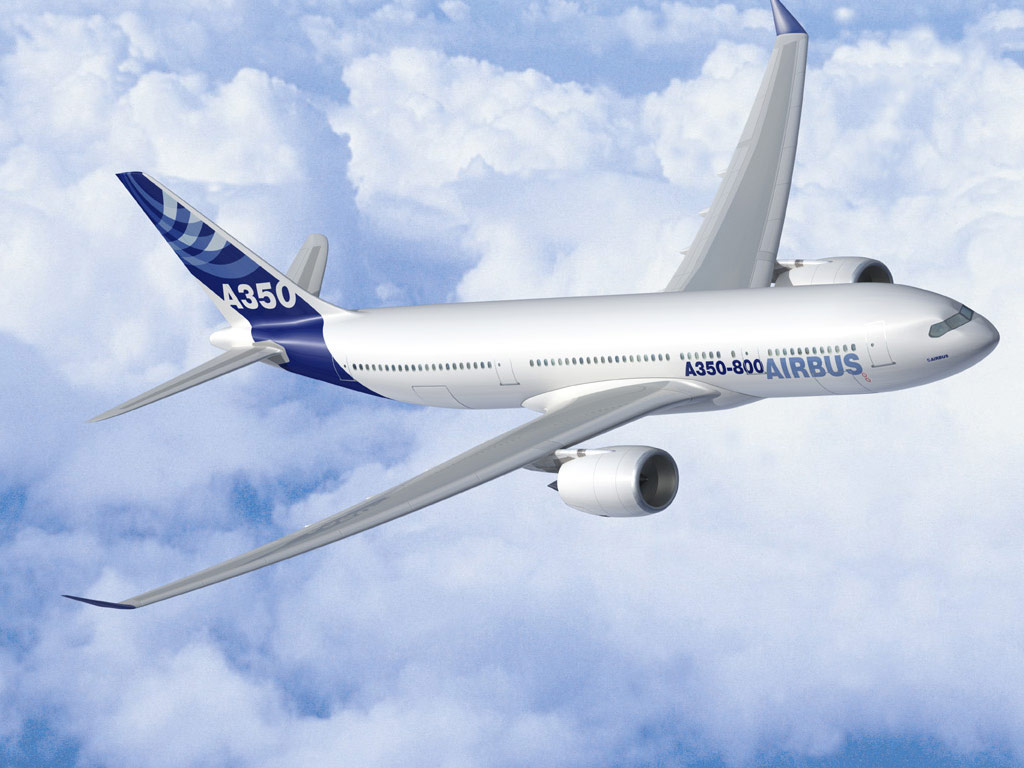
\includegraphics[width=0.25\textwidth]{Figures/Airbus_A350.jpg}
%  \caption[Caption for figure in TOC.]{Caption for figure.}
%  \label{fig:airbus1}
%\end{figure}
%
%\begin{figure}[!htb]
%  \begin{subfigmatrix}{2}
%    \subfigure[Airbus A320]{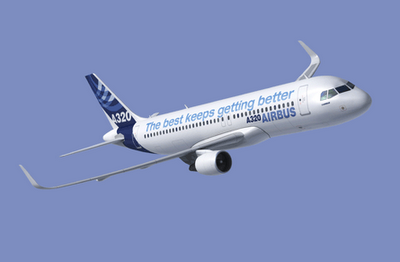
\includegraphics[width=0.49\linewidth]{Figures/Airbus_A320_sharklets.png}}
%    \subfigure[Bombardier CRJ200]{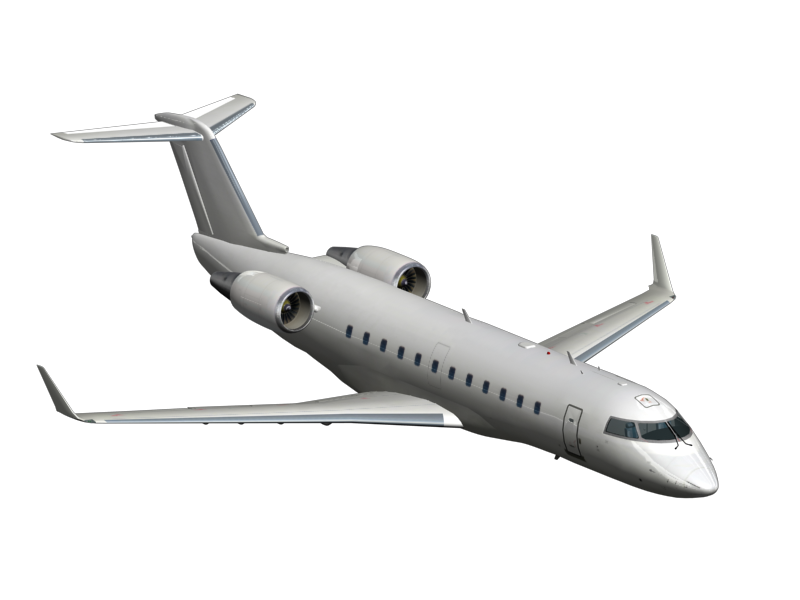
\includegraphics[width=0.49\linewidth]{Figures/Bombardier_CRJ200.png}}
%  \end{subfigmatrix}
%  \caption{Some aircrafts.}
%  \label{fig:aircrafts}
%\end{figure}
%
%Make reference to Figures \ref{fig:airbus1} and \ref{fig:aircrafts}.
%
%By default, the supported file types are {\it .png,.pdf,.jpg,.mps,.jpeg,.PNG,.PDF,.JPG,.JPEG}.
%
%See \url{http://mactex-wiki.tug.org/wiki/index.php/Graphics_inclusion} for adding support to other extensions.
%
%
%% ----------------------------------------------------------------------
%\subsubsection{Drawings}
%\label{subsection:drawings}
%
%Insert your subsection material and for instance a few drawings...
%
%The schematic illustrated in Fig.~\ref{fig:algorithm} can represent some sort of algorithm.
%
%\begin{figure}[!htb]
%  \centering
%  \scriptsize
%%  \footnotesize 
%%  \small
%  \setlength{\unitlength}{0.9cm}
%  \begin{picture}(8.5,6)
%    \linethickness{0.3mm}
%
%    \put(3,6){\vector(0,-1){1}}
%    \put(3.5,5.4){$\bf \alpha$}
%    \put(3,4.5){\oval(6,1){}}
%    %\put(0,4){\framebox(6,1){}}
%    \put(0.3,4.4){Grid Generation: \quad ${\bf x} = {\bf x}\left({\bf \alpha}\right)$}
%
%    \put(3,4){\vector(0,-1){1}}
%    \put(3.5,3.4){$\bf x$}
%    \put(3,2.5){\oval(6,1){}}
%    %\put(0,2){\framebox(6,1){}}
%    \put(0.3,2.4){Flow Solver: \quad ${\cal R}\left({\bf x},{\bf q}\left({\bf x}\right)\right) = 0$}
%
%    \put(6.0,2.5){\vector(1,0){1}}
%    \put(6.4,3){$Y_1$}
%
%    \put(3,2){\vector(0,-1){1}}
%    \put(3.5,1.4){$\bf q$}
%    \put(3,0.5){\oval(6,1){}}
%    %\put(0,0){\framebox(6,1){}}
%    \put(0.3,0.4){Structural Solver: \quad ${\cal M}\left({\bf x},{\bf q}\left({\bf x}\right)\right) = 0$}
%
%    \put(6.0,0.5){\vector(1,0){1}}
%    \put(6.4,1){$Y_2$}
%
%    %\put(7.8,2.5){\oval(1.6,5){}}
%    \put(7.0,0){\framebox(1.6,5){}}
%    \put(7.1,2.5){Optimizer}
%    \put(7.8,5){\line(0,1){1}}
%    \put(7.8,6){\line(-1,0){4.8}}
%  \end{picture}
%  \caption{Schematic of some algorithm.}
%  \label{fig:algorithm}
%\end{figure}
%
%
%% ----------------------------------------------------------------------
%\subsection{Equations}
%\label{subsection:equations}
%
%Equations can be inserted in different ways.
%
%The simplest way is in a separate line like this
%
%\begin{equation}
%  \frac{{\rm d} q_{ijk}}{{\rm d} t} + {\cal R}_{ijk}({\bf q}) = 0 \,.
%\label{eq:ode}
%\end{equation}
%
%If the equation is to be embedded in the text. One can do it like this ${\partial {\cal R}}/{\partial {\bf q}}=0$.
%
%It may also be split in different lines like this
%
%\begin{eqnarray}
%  {\rm Minimize}   && Y({\bf \alpha},{\bf q}({\bf \alpha}))            \nonumber           \\
%  {\rm w.r.t.}     && {\bf \alpha} \,,                                 \label{eq:minimize} \\
%  {\rm subject~to} && {\cal R}({\bf \alpha},{\bf q}({\bf \alpha})) = 0 \nonumber           \\
%                   &&       C ({\bf \alpha},{\bf q}({\bf \alpha})) = 0 \,. \nonumber
%\end{eqnarray}
%
%It is also possible to use subequations. Equations~\ref{eq:continuity}, \ref{eq:momentum} and \ref{eq:energy} form the Naver--Stokes equations~\ref{eq:NavierStokes}.
%
%\begin{subequations}
%    \begin{equation}
%    \frac{\partial \rho}{\partial t} + \frac{\partial}{\partial x_j}\left( \rho u_j \right) = 0 \,,
%    \label{eq:continuity}
%    \end{equation}
%    \begin{equation}
%    \frac{\partial}{\partial t}\left( \rho u_i \right) + \frac{\partial}{\partial x_j} \left( \rho u_i u_j + p \delta_{ij} - \tau_{ji} \right) = 0, \quad i=1,2,3 \,,
%    \label{eq:momentum}
%    \end{equation}
%    \begin{equation}
%        \frac{\partial}{\partial t}\left( \rho E \right) + \frac{\partial}{\partial x_j} \left( \rho E u_j + p u_j - u_i \tau_{ij} + q_j \right) = 0 \,.
%    \label{eq:energy}
%    \end{equation}
%\label{eq:NavierStokes}%
%\end{subequations}
%
%
%% ----------------------------------------------------------------------
%\subsection{Tables}
%\label{section:tables}
%
%Insert your subsection material and for instance a few tables...
%
%Make sure all tables presented are referenced in the text!
%
%Follow some guidelines when making tables:
%
%\begin{itemize}
%  \item Avoid vertical lines
%  \item Avoid “boxing up” cells, usually 3 horizontal lines are enough: above, below, and after heading
%  \item Avoid double horizontal lines
%  \item Add enough space between rows
%\end{itemize}
%
%\begin{table}[!htb]
%  \renewcommand{\arraystretch}{1.2} % more space between rows
%  \centering
%  \begin{tabular}{lccc}
%    \toprule
%    Model           & $C_L$ & $C_D$ & $C_{M y}$ \\
%    \midrule
%    Euler           & 0.083 & 0.021 & -0.110    \\
%    Navier--Stokes  & 0.078 & 0.023 & -0.101    \\
%    \bottomrule
%  \end{tabular}
%  \caption[Table caption shown in TOC.]{Table caption.}
%  \label{tab:aeroCoeff}
%\end{table}
%
%Make reference to Table \ref{tab:aeroCoeff}.
%
%Tables \ref{tab:memory} and \ref{tab:multipleColumns} are examples of tables with merging columns:
%
%\begin{table}[!htb]
%  \renewcommand{\arraystretch}{1.2} % more space between rows
%  \centering
%  \begin{tabular}[]{lrr}
%    \toprule
%                & \multicolumn{2}{c}{\underline{Virtual memory [MB]}} \\
%                & Euler       & Navier--Stokes \\
%    \midrule
%      Wing only &  1,000      &    2,000       \\
%      Aircraft  &  5,000      &   10,000       \\
%      (ratio)   & $5.0\times$ & $5.0\times$    \\
%    \bottomrule
%  \end{tabular}
%  \caption{Memory usage comparison (in MB).}
%  \label{tab:memory}
%\end{table}
%
%\begin{table}[!htb]
%  \centering
%  \renewcommand{\arraystretch}{1.2} % more space between rows
%  \begin{tabular}{@{}rrrrcrrr@{}} % remove space to the vertical edges @{}...@{}
%    \toprule
%      & \multicolumn{3}{c}{$w = 2$} & \phantom{abc} & \multicolumn{3}{c}{$w = 4$} \\
%    \cmidrule{2-4}
%    \cmidrule{6-8}
%      & $t=0$ & $t=1$ & $t=2$ && $t=0$ & $t=1$ & $t=2$ \\
%    \midrule
%      $dir=1$
%      \\
%      $c$ &  0.07 &  0.16 &  0.29 &&  0.36 &  0.71 &   3.18 \\
%      $c$ & -0.86 & 50.04 &  5.93 && -9.07 & 29.09 &  46.21 \\
%      $c$ & 14.27 &-50.96 &-14.27 && 12.22 &-63.54 &-381.09 \\
%      $dir=0$
%      \\
%      $c$ &  0.03 &  1.24 &  0.21 &&  0.35 & -0.27 &  2.14 \\
%      $c$ &-17.90 &-37.11 &  8.85 &&-30.73 & -9.59 & -3.00 \\
%      $c$ &105.55 & 23.11 &-94.73 &&100.24 & 41.27 &-25.73 \\
%    \bottomrule
%  \end{tabular}
%  \caption{Another table caption.}
%  \label{tab:multipleColumns}
%\end{table}
%
%An example with merging rows can be seen in Tab.\ref{tab:multipleRows}.
%
%\begin{table}[!htb]
%  \renewcommand{\arraystretch}{1.2} % more space between rows
%  \centering
%  \begin{tabular}{ccccc}
%    \toprule
%      \multirow{2}{*}{ABC} & \multicolumn{4}{c}{header} \\
%      \cmidrule{2-5} & 1.1 & 2.2 & 3.3 & 4.4 \\
%    \midrule
%      \multirow{2}{*}{IJK} & \multicolumn{2}{c}{\multirow{2}{*}{group}} & 0.5 & 0.6 \\
%      \cmidrule{4-5}       & \multicolumn{2}{c}{}                       & 0.7 & 1.2 \\
%    \bottomrule
%  \end{tabular}
%  \caption{Yet another table caption.}
%  \label{tab:multipleRows}
%\end{table}
%
%If the table has too many columns, it can be scaled to fit the text widht, as in Tab.\ref{tab:scale}.
%\begin{table}[!htb]
%  \renewcommand{\arraystretch}{1.2} % more space between rows
%  \centering
%  \resizebox*{\textwidth}{!}{%
%    \begin{tabular}[]{lcccccccccc}
%      \toprule
%        Variable &  a  &  b  &  c  &  d  &  e  &  f  &  g  &  h  &  i  &  j  \\
%      \midrule
%        Test 1   &  10,000 &  20,000 &  30,000 &  40,000 &  50,000 &  60,000 &  70,000 &  80,000 &  90,000 & 100,000 \\
%        Test 2   &  20,000 &  40,000 &  60,000 &  80,000 & 100,000 & 120,000 & 140,000 & 160,000 & 180,000 & 200,000 \\
%      \bottomrule
%    \end{tabular}
%  }%
%  \caption{Very wide table.}
%  \label{tab:scale}%
%\end{table}
%
%
%% ----------------------------------------------------------------------
%\subsection{Mixing}
%\label{section:mixing}
%
%If necessary, a figure and a table can be put side-by-side as in Fig.\ref{fig:side_by_side}
%
%\begin{figure}[!htb]
%  \begin{minipage}[b]{0.60\linewidth}
%    \centering
%    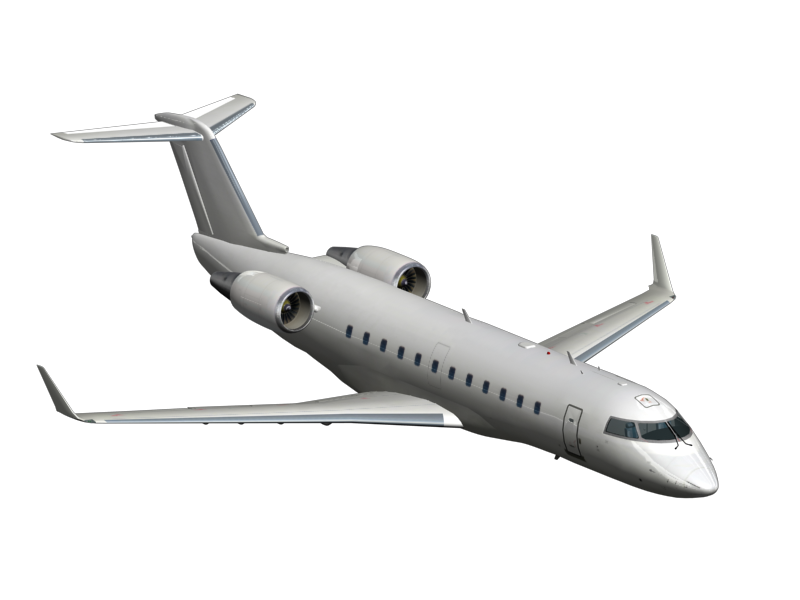
\includegraphics[width=\linewidth]{Figures/Bombardier_CRJ200}
%  \end{minipage}%
%  \begin{minipage}[b]{0.30\linewidth}
%    \centering
%    \begin{tabular}[b]{lll}
%      \toprule
%        \multicolumn{3}{c}{Legend} \\
%      \midrule
%        A & B & C \\
%        0 & 0 & 0 \\
%        0 & 1 & 0 \\
%        1 & 0 & 0 \\
%        1 & 1 & 1 \\
%      \bottomrule
%    \end{tabular}
%    \vspace{5em}
%  \end{minipage}
%\caption{Figure and table side-by-side.}
%\label{fig:side_by_side}
%\end{figure}


\clearpage

%\input{Thesis_new_file} % add new .tex files for new chapters
% \cleardoublepage

%\input{Thesis_new_file} % add new .tex files for new chapters
% \cleardoublepage

%%%%%%%%%%%%%%%%%%%%%%%%%%%%%%%%%%%%%%%%%%%%%%%%%%%%%%%%%%%%%%%%%%%%%%%%%
%                                                                      %
%     File: Thesis_Results.tex                                         %
%     Tex Master: Thesis.tex                                           %
%                                                                      %
%     Author: Andre C. Marta                                           %
%     Last modified :  2 Jul 2015                                      %
%                                                                      %
%%%%%%%%%%%%%%%%%%%%%%%%%%%%%%%%%%%%%%%%%%%%%%%%%%%%%%%%%%%%%%%%%%%%%%%%

\chapter{Results}
\label{chapter:results}

In this chapter we describe the main results of the search for $hh\rightarrow b\overline{b}b\overline{b}$ at the FCC-hh using two benchmark luminosities, $30~\text{ab}^{-1}$ and $3~\text{ab}^{-1}$ (section \ref{sec:dihiggs_FCC}). The statistical analysis used to extract the signal strength and to set limits on the Higgs boson triple coupling is also discussed. In section \ref{sec:gran_studies} we show how the significance of the analysis varies as a function of the granularity of the HCAL and/or the detector configuration. We also compare the results obtained using particle flow and pure calorimeter jets.

\section{Di-Higgs discovery potential at the FCC-hh}
\label{sec:dihiggs_FCC}

The event selection of the baseline analysis for the search for $hh\rightarrow b\overline{b}b\overline{b}$ at the FCC with the baseline detector design is summarized in tables \ref{table:cutflow_sig_FCC} and \ref{table:cutflow_bkg_FCC} for the signal samples (SM, DM mediator and type II 2HDM) and for the background samples ($4b+j$, $jj+0/1/2 j$ and $t\overline{t}$), respectively.

From table \ref{table:cutflow_sig_FCC}, we see that for the BSM models, the signal efficiency is higher than for the SM. It goes from $0.422$ in the SM, to $0.487$ in the DM mediator model and to $1.342$ in the type II 2HDM.

Considering the SM production of Higgs pairs, the achieved significance is
\begin{equation}
	S/\sqrt{B}=6.8\pm 0.7\quad (2.15\pm 0.27)
\end{equation}
for an integrated luminosity of $30(3)~\text{ab}^{-1}$. For $\mathcal{L}=30~\text{ab}^{-1}$, the significance is above the $5\sigma$ threshold while for $\mathcal{L}=3~\text{ab}^{-1}$ it is above the $3\sigma$ threshold. These results indicated that with the entire dataset that is expected to be accumulated by the FCC-hh detector it should be possible to observe the production of Higgs pairs.

For a signal model that includes a $1$ TeV dark matter mediator that can decay to pairs of SM Higgs bosons the achieve significance is $1.48\pm0.15(0.47\pm0.05)$ for an integrated luminosity of $30(3)~\text{ab}^{-1}$. The significance is well bellow the $3\sigma$ threshold for both luminosities. Therefore, from the point of view of enhancing Higgs pair production with respect to the SM, this model is not very interesting. In this model, the coupling of the DM mediator to the Higgs pairs is small which means that the contribution from the box diagram dominates over the resonant production (s-channel diagram), just like in the SM. 

For the type II 2HDM the achieved significance is
\begin{equation}
	S/\sqrt{B}=8.7\pm 0.9(2.76\pm 0.28)
\end{equation}
for an integrated luminosity of $30(3)~\text{ab}^{-1}$. The high efficiency of this signal sample through the cuts, reflected in the high significance that is achieved, make it a very interesting model from the point of view of Higgs pair production.   

%\begin{table}
%	\begin{tabular}{lcccccccccc}
%		\toprule 
%		\textbf{Selection} & SM & $\epsilon(\%)$ & 2HDM & $\epsilon(\%)$ & 4b+j & $\epsilon(\%)$& jj+0/1/2 j &$\epsilon(\%)$& $t\overline{t}$+0/1/2 j & $\epsilon(\%)$\\
%		\midrule
%		Gen level & $3.46\text{e}7$ & $100$& $5.55\text{e}7$ & $100$&$4.90\text{e}10$ & $100$&$5.47\text{e}14$ &$100$ &$2.25\text{e}12$&$100$\\
%		\rowcolor{black!10}N(b-tags)$\geq4$ & $3.20\text{e}7$& $92.5$ & $5.09\text{e}7$& $91.8$& $3.72\text{e}10$ & $75.8$ &$2.17\text{e}13$ & $3.963$&$1.20\text{e}12$& $53.5$\\
%		$p_T(j_1,j_2)\geq200$ GeV & $5.75\text{e}6$ & $16.6$ & $1.70\text{e}7$& $30.6$&$8.73\text{e}9$ & $17.8$& $4.06\text{e}12$ &$0.74$ &$2.38\text{e}10$ & $1.06$\\
%		\rowcolor{black!10}$p_T(j_1)\geq 400$ GeV & $2.99\text{e}6$ & $8.623$ & $1.01\text{e}7$& $18.2$&$3.44\text{e}9$ & $7.0$ &$1.00\text{e}12$ & $0.18$ &$1.00\text{e}10$& $0.446$\\
%		$p_T(j_2)\geq 350$ GeV & $1.98\text{e}6$ & $5.7$ & $6.22\text{e}6$& $11.2$ &$1.93\text{e}9$ &$3.9$ &$6.61\text{e}11$ &$0.121$ &$5.92\text{e}9$& $0.263$\\
%		\rowcolor{black!10}$p_T(j_1+j_2)\geq 100$ GeV & $1.61\text{e}6$& $4.648$& $4.53\text{e}6$& $8.16$&$1.62\text{e}9$& $3.3$&$3.80\text{e}11$ & $0.07$ & $5.03\text{e}9$& $0.223$\\
%		$\tau_{21}(j_1,j_2)<0.55$ & $5.91\text{e}5$ & $1.7$ &$1.85\text{e}6$ &$3.3$&$2.65\text{e}8$ & $0.54$ & $2.95\text{e}10$ & $0.005$ & $1.56\text{e}9$ & $0.069$\\
%		\rowcolor{black!10}$FW2(j_1)>0.2$ &$4.44\text{e}5$ & $1.28$& $1.50\text{e}6$& $2.7$&$1.57\text{e}8$ & $ 0.32$&$1.78\text{e}10$ & $0.003$& $4.41\text{e}8$& $0.020$\\
%		$100<M_{SD}(j1,j2)<135$ GeV & $1.46\text{e}5$&$0.422$ &$6.07\text{e}5$ & $1.09$& $6.66\text{e}6$& $0.0136$ & $4.38\text{e}8$ & $0.00008$ & $1.75\text{e}7$& $0.00078$\\
%		\bottomrule
%	\end{tabular}
%	\caption{FCC default HCAL. Entries normalized to $\mathcal{L}=30~\text{ab}^{-1}$}
%\end{table}

\begin{table}
	\centering
	\caption{Cumulative efficiency, in percentage, of each event selection criterion for the signal samples (SM and 2HDM). The absolute value of expected events after some key selection cuts is shown in curved brackets. The number of expected events is normalized to $\mathcal{L}=30~\text{ab}^{-1}$. The double horizontal line marks the pre-selection cuts. These results were obtained using the FCC-hh baseline detector design, as implemented in Delphes by the FCC-hh study group.\newline}
	\label{table:cutflow_sig_FCC}
	\begin{tabular}{lccc}
		\toprule 
		\textbf{Selection [FCC-hh]} & SM  & DM mediator &2HDM type II\\
		\midrule
		\multirow{2}{*}{Gen level} & $100$ & $100$ &$100$ \\
		&  $(34638\pm16)\times 10^3$ & $(65400\pm29)\times 10^2$ & $(13977\pm7)\times 10^3$ \\
		\rowcolor{black!10}N(b-tags)$\geq4$ & $92.488$ & $92.593$ &$93.430$\\
		\multirow{2}{*}{$p_T(j_1,j_2)\geq200$ GeV} & $16.6602$ & $17.033$ &$58.860$ \\ 
		& $(5751\pm6)\times 10^3$ & $(11140\pm12)\times 10^2$ & $8227\pm5\times 10^3$\\
		\midrule \midrule
		\rowcolor{black!10}$p_T(j_1)\geq 400$ GeV & $8.623$ & $9.156$ &$21.041$\\ 
		$p_T(j_2)\geq 350$ GeV & $5.709$ &$6.161$&  $13.202$ \\
		\rowcolor{black!10}$p_T(j_1+j_2)\geq 100$ GeV &  $4.648$&$4.968$ &  $9.624$\\
		$\tau_{21}(j_1,j_2)<0.55$ & $1.705$&$1.878$ &$4.057$\\
		\rowcolor{black!10}$FW2(j_1)>0.2$ & $1.281$&$1.421$& $3.267$\\
		\multirow{2}{*}{$(100<M_{SD}(j1,j2)<135)$ GeV} & $0.422$ & $0.487$&$1.342$\\
		&$(1463\pm10)\times 10^2$&$(3188\pm20)\times10$&$(1876\pm8)\times 10^2$\\
		\bottomrule
	\end{tabular}
\end{table}

\begin{table}
	\centering
	\caption{Cumulative efficiency, in percentage, of each event selection criterion for the background samples ($4b+j$, $jj+0/1/2 j$ and $t\overline{t}$+0/1/2 j). The absolute value of expected events after some key selection cuts is shown in curved brackets. The number of expected events is normalized to $\mathcal{L}=30~\text{ab}^{-1}$. The double horizontal line marks the pre-selection cuts. These results were obtained using the FCC-hh baseline detector design, as implemented in Delphes by the FCC-hh study group.\newline}
	\label{table:cutflow_bkg_FCC}
	\begin{tabular}{lccc}
		\toprule 
		\textbf{Selection [FCC-hh]} & $4b+j$  & $jj+0/1/2 j$ & $t\overline{t}$ \\
		\midrule
		\multirow{2}{*}{Gen level} & $100$ & $100$ &$100$ \\
		&  $(49035\pm12)\times 10^6$ & $(54698\pm17)\times 10^{10}$ & $(22503\pm11)\times 10^8$ \\
		\rowcolor{black!10}N(b-tags)$\geq4$ & $75.819$ & $3.963$ &$53.495$\\
		\multirow{2}{*}{$p_T(j_1,j_2)\geq200$ GeV} & $17.811$ & $0.742$ &$1.056$ \\ 
		& $(8734\pm5)\times 10^6$ & $(4058\pm14)\times 10^9$ & $(2377\pm11)\times 10^7$\\
		\midrule \midrule
		\rowcolor{black!10}$p_T(j_1)\geq 400$ GeV & $7.008$ & $0.183$ &$0.446$\\ 
		$p_T(j_2)\geq 350$ GeV & $3.928$ &$0.121$&  $0.263$ \\
		\rowcolor{black!10}$p_T(j_1+j_2)\geq 100$ GeV &  $3.311$&$0.070$ &  $0.223$\\
		$\tau_{21}(j_1,j_2)<0.55$ & $0.540$&$0.005$ &$0.069$\\
		\rowcolor{black!10}$FW2(j_1)>0.2$ & $0.320$&$0.003$& $0.020$\\
		\multirow{2}{*}{$(100<M_{SD}(j1,j2)<135)$ GeV} & $0.014$ & $0.00008$&$0.0008$\\
		&$(666\pm13)\times 10^4$&$(4\pm4)\times10^8$&$(175\pm30)\times 10^5$\\
		\bottomrule
	\end{tabular}
\end{table}

\subsection{Statistical analysis}

\subsection{Comparing with the ATLAS detector}

The event selection of the search for $hh\rightarrow b\overline{b}b\overline{b}$ with the ATLAS detector at a CM energy of $100$ TeV is summarized in tables \ref{table:cutflow_sig_ATLAS} and \ref{table:cutflow_bkg_ATLAS} for the signal and background samples, respectively.

It is interesting to compare the results obtained with the FCC-hh default detector simulation with the ones obtained using the simulation of the ATLAS detector. These are summarized in table \ref{table:FCC_ATLAS_comp} in terms of the achieved significance for an integrated luminosity of $30~\text{ab}^{-1}$.

For all the signal models, the significance increases approximately $20\%$ going from the ATLAS detector to the FCC-hh. For the SM signal, Nonetheless, using the ATLAS default detector configuration the achieved significance is already above $5\sigma$: $S/\sqrt{B}=5.6\pm 0.6$.

\begin{table}
	\centering
	\caption{Cumulative efficiency, in percentage, of each event selection criterion for the signal samples (SM and 2HDM). The absolute value of expected events after some key selection cuts is shown in curved brackets. The number of expected events is normalized to $\mathcal{L}=30~\text{ab}^{-1}$. The double horizontal line marks the pre-selection cuts. These results were obtained using the ATLAS detector design, as implemented in Delphes.\newline}
	\label{table:cutflow_sig_ATLAS}
	\begin{tabular}{lccc}
		\toprule 
		\textbf{Selection [ATLAS]} & SM  & DM mediator &2HDM type II\\
		\midrule
		\multirow{2}{*}{Gen level} & $100$ & $100$ &$100$ \\
		&  $(34638\pm16)\times 10^3$ & $(65400\pm29)\times 10^2$ &  \\
		\rowcolor{black!10}N(b-tags)$\geq4$ & $88.691$ & $88.787$ &\\
		\multirow{2}{*}{$p_T(j_1,j_2)\geq200$ GeV} & $15.534$ & $15.94$ & \\ 
		& $(5381\pm6)\times 10^3$ & $(10426\pm12)\times 10^2$ & \\
		\midrule \midrule
		\rowcolor{black!10}$p_T(j_1)\geq 400$ GeV & $7.997$ & $8.499$ &\\ 
		$p_T(j_2)\geq 350$ GeV & $5.283$ &$5.704$&  \\
		\rowcolor{black!10}$p_T(j_1+j_2)\geq 100$ GeV &  $4.305$&$4.604$ &  \\
		$\tau_{21}(j_1,j_2)<0.55$ & $1.648$&$1.809$ &\\
		\rowcolor{black!10}$FW2(j_1)>0.2$ & $1.125$&$1.243$& \\
		\multirow{2}{*}{$(100<M_{SD}(j1,j2)<135)$ GeV} & $0.323$ & $0.374$&\\
		&$(1119\pm9)\times 10^2$&$(2446\pm18)\times10$&\\
		\bottomrule
	\end{tabular}
\end{table}

\begin{table}
	\centering
	\caption{Cumulative efficiency, in percentage, of each event selection criterion for the background samples ($4b+j$, $jj+0/1/2 j$ and $t\overline{t}$+0/1/2 j). The absolute value of expected events after some key selection cuts is shown in curved brackets. The number of expected events is normalized to $\mathcal{L}=30~\text{ab}^{-1}$. The double horizontal line marks the pre-selection cuts. These results were obtained using the ATLAS detector design, as implemented in Delphes.\newline}
	\label{table:cutflow_bkg_ATLAS}
	\begin{tabular}{lccc}
		\toprule 
		\textbf{Selection [ATLAS]} & $4b+j$  & $jj+0/1/2 j$ & $t\overline{t}$ \\
		\midrule
		\multirow{2}{*}{Gen level} & $100$ & $100$ &$100$ \\
		&  $(49035\pm15)\times 10^6$ & $(54698\pm15)\times 10^{10}$ & $(22503\pm9)\times 10^8$ \\
		\rowcolor{black!10}N(b-tags)$\geq4$ & $71.617$ & $3.747$ &$51.782$\\
		\multirow{2}{*}{$p_T(j_1,j_2)\geq200$ GeV} & $16.301$ & $0.767$ &$0.984$ \\ 
		& $(7993\pm6)\times 10^6$ & $(4193\pm12)\times 10^9$ & $(2215\pm9)\times 10^7$\\
		\midrule \midrule
		\rowcolor{black!10}$p_T(j_1)\geq 400$ GeV & $6.378$ & $0.170$ &$0.416$\\ 
		$p_T(j_2)\geq 350$ GeV & $3.560$ &$0.112$&  $0.245$ \\
		\rowcolor{black!10}$p_T(j_1+j_2)\geq 100$ GeV &  $3.000$&$0.064$ &  $0.206$\\
		$\tau_{21}(j_1,j_2)<0.55$ & $0.545$&$0.008$ &$0.064$\\
		\rowcolor{black!10}$FW2(j_1)>0.2$ & $0.272$&$0.003$& $0.016$\\
		\multirow{2}{*}{$(100<M_{SD}(j1,j2)<135)$ GeV} & $0.010$ & $0.00007$&$0.0007$\\
		&$(496\pm14)\times 10^4$&$(37\pm30)\times10^7$&$(165\pm25)\times 10^5$\\
		\bottomrule
	\end{tabular}
	
\end{table}

\begin{table}
	\centering
	\caption{oi\newline}
	\label{table:FCC_ATLAS_comp}
	\begin{tabular}{lcc}
		\toprule 
		\textbf{Signal sample} & ATLAS  & FCC-hh  \\
		\midrule
		SM & $5.6\pm 0.6$ & $6.8\pm 0.7$ \\
		\rowcolor{black!10}1 TeV DM mediator & $1.23\pm0.12$ & $1.48\pm0.15$ \\
		2HDM type II & $7.2\pm 0.7$ &  $8.7\pm0.9$\\ 
		\bottomrule

	\end{tabular}
	
\end{table}


\section{Hadronic calorimeter granularity studies for future colliders}
\label{sec:gran_studies}

In this section we present the results that allow us to compare the different detector configurations.

The softdrop mass of the leading Higgs candidate for the SM signal sample is shown on the left of figure \ref{fig:CompGran} for the different detector configurations. We see that the mass resolution increases as we increase the granularity [QUANTIFY?].

The $\tau_{21}$ variable for the leading Higgs candidate for the SM signal (filled lines) and for the $4b+j$ background (dashed lines) is shown on the right of figure \ref{fig:CompGran} for the different detector configurations. The overlap between the signal and background distributions decreases as the granularity of the HCAL increases. This means that the separation between signal and background increases. This was expected because an increase in the granularity of the hadronic calorimeter should help resolve better the substructure of boosted jets. For the $4b+j$ background the maximum overlap fraction is $0.68\pm0.12$ for the ATLAS detector and for the ATLAS HCAL. The minimum is $0.67\pm0.12$ for the remaining configurations. For the multijet background the maximum overlap is $0.55\pm0.10$ for the ATLAS detector and the minimum is $0.50\pm0.09$ for the FCC-hh default detector, with an HCAL two times less granular in $\phi$ and with an HCAL two times more granular in $\eta$ and $\phi$. For the $t\overline{t}$, the overlap is $0.78\pm0.13$ for all configurations except for the FCC-hh default configuration for which it is $0.77\pm0.13$. Regardless of the background, the overlap area between the distributions changes very little for different detector configurations. The multijet background has the smallest overlap, as expected. 

Figures \ref{fig:EffvsGran} show the signal efficiency for three signal models: SM (filled squares), $1$ TeV DM mediator (empty squares) and type II 2HDM with $m_H=900$ GeV, for eflow (left) and HCAL jets (right). 

For eflow jets the efficiency increases as we increase the granularity, for all signal models. For HCAL jets there is a more complex dependence [WHY?].

The efficiency is higher for both BSM models than for the SM. This is because these models were chosen to have very heavy particles decaying to a pair of highly boosted Higgs pairs.

The significances achieved with the optimized analysis as a function of the detector configuration for the SM signal, the DM mediator model and the type II 2HDM are shown in figure \ref{fig:SSBvsGran1} on the left and right and on figure \ref{fig:SSBvsGran_2HDM}, respectively. The uncertainty associated with each value of the significance is computed using standard error propagation. Only the statistical error is taken in to account.

Motivated by the small change in significance over the range of configurations that were tested we implemented exactly the same analysis but using HCAL jets instead of eflow jets. The results are shown in the same plots using triangular markers. On the one hand, the achieved significance is always smaller when using HCAL jets because we are not making use of the tracking information. On the other hand, when using HCAL jets, the significance changes a lot more over the configuration range. In particular, it increases as the HCAL granularity is increased. [QUANTIFY]

The small change in the significance when using eflow jets and the fact the change increases when using HCAL jets indicate that in the FCC-hh baseline detector design the resolution of the tracking system is so good, in particular, so much better than the HCAL resolution [NUMBERS] that it is the limiting factor.

[COMPARE THE DIFFERENT SIGNAL SAMPLES IN TERMS OF THE CHANGE IN SIGNIFICANCE]

\begin{figure}
	\centering
	\begin{minipage}{.5\textwidth}
		\centering
		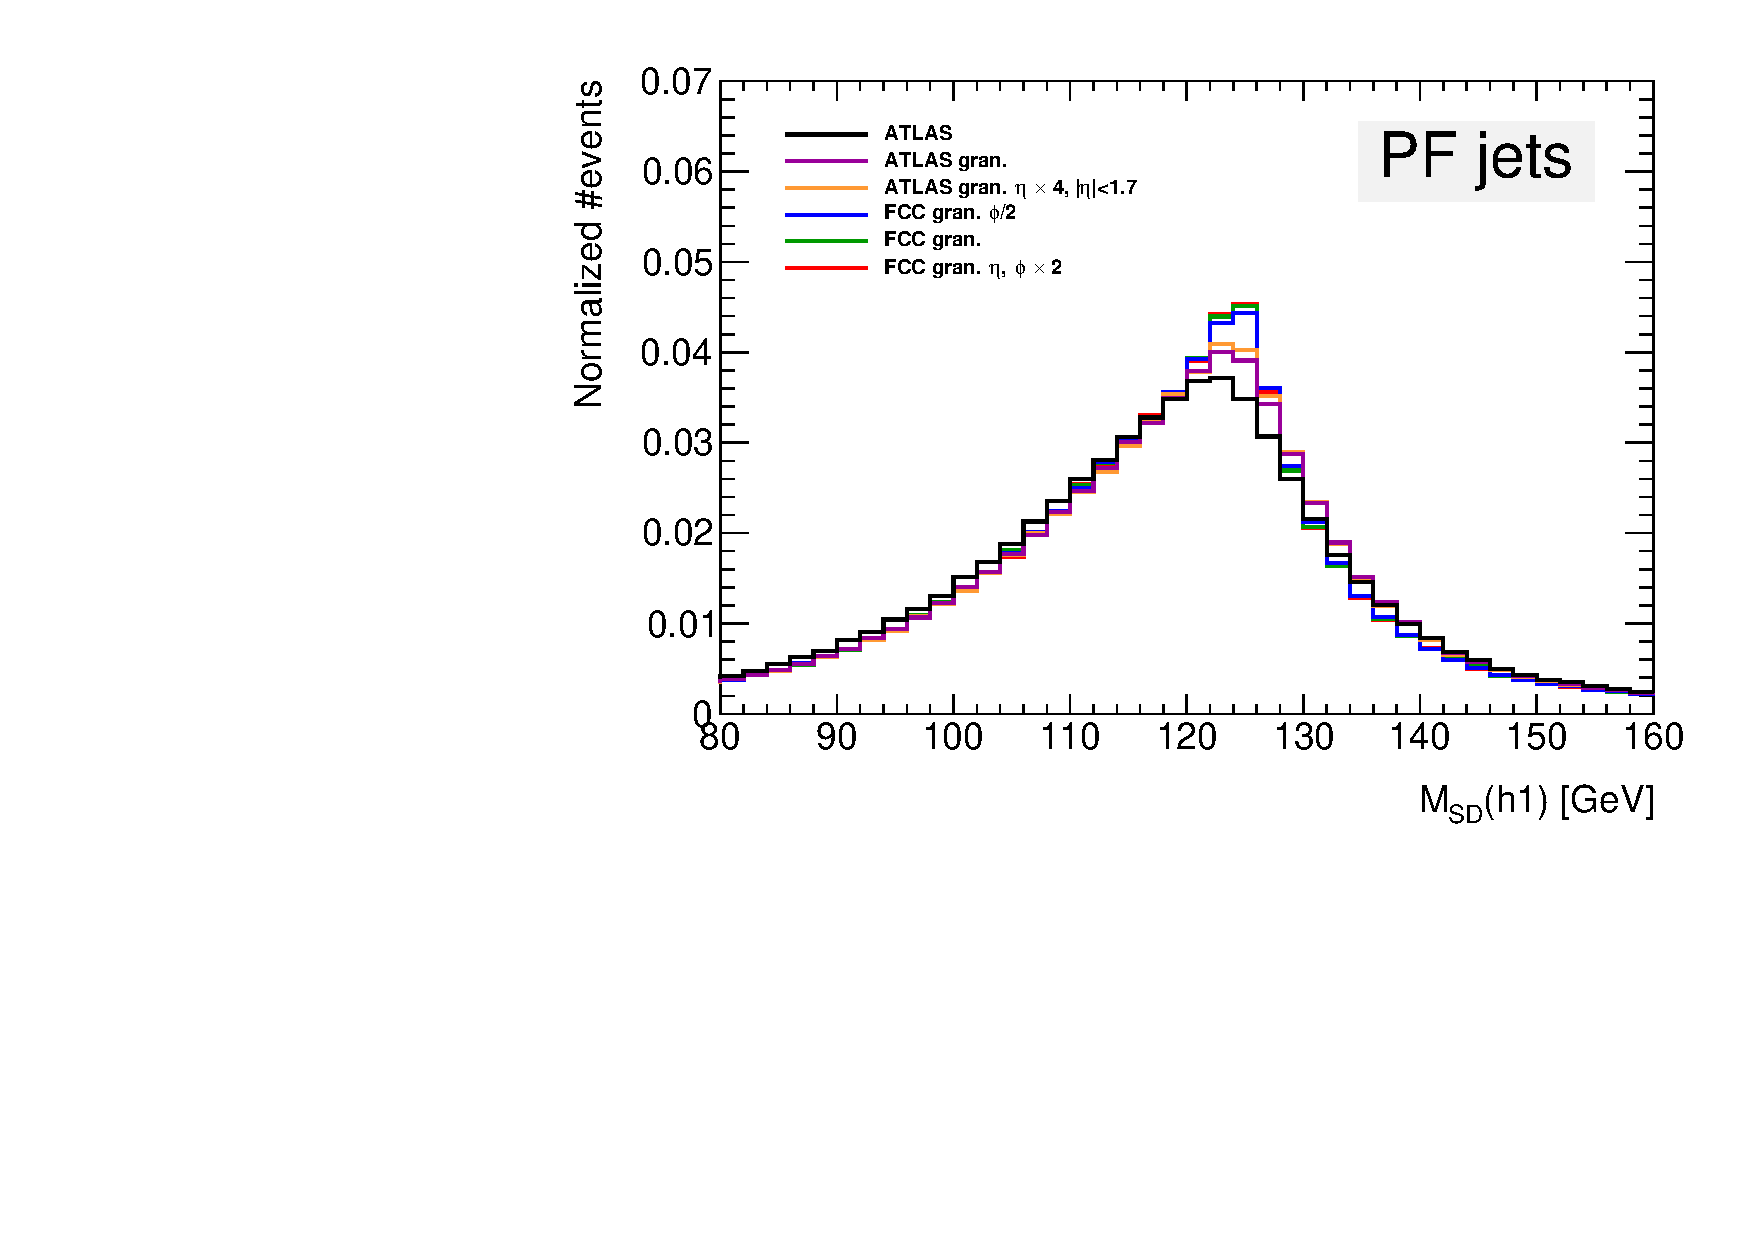
\includegraphics[trim={.65cm 0 0 0},clip,width=\linewidth]{./Figures/M.pdf}
		\label{fig:CompGran_M}
		%\caption{Leading Higgs candidate softdrop mass plot for the different detector configurations for the SM signal sample. This plot contains all the signal events that passed all the cuts of the baseline analysis. Note that the x axis range is from $80$ GeV to $160$ GeV in order to make the differences between the histograms more clear.}
	\end{minipage}%
	\begin{minipage}{.5\textwidth}
		\centering
		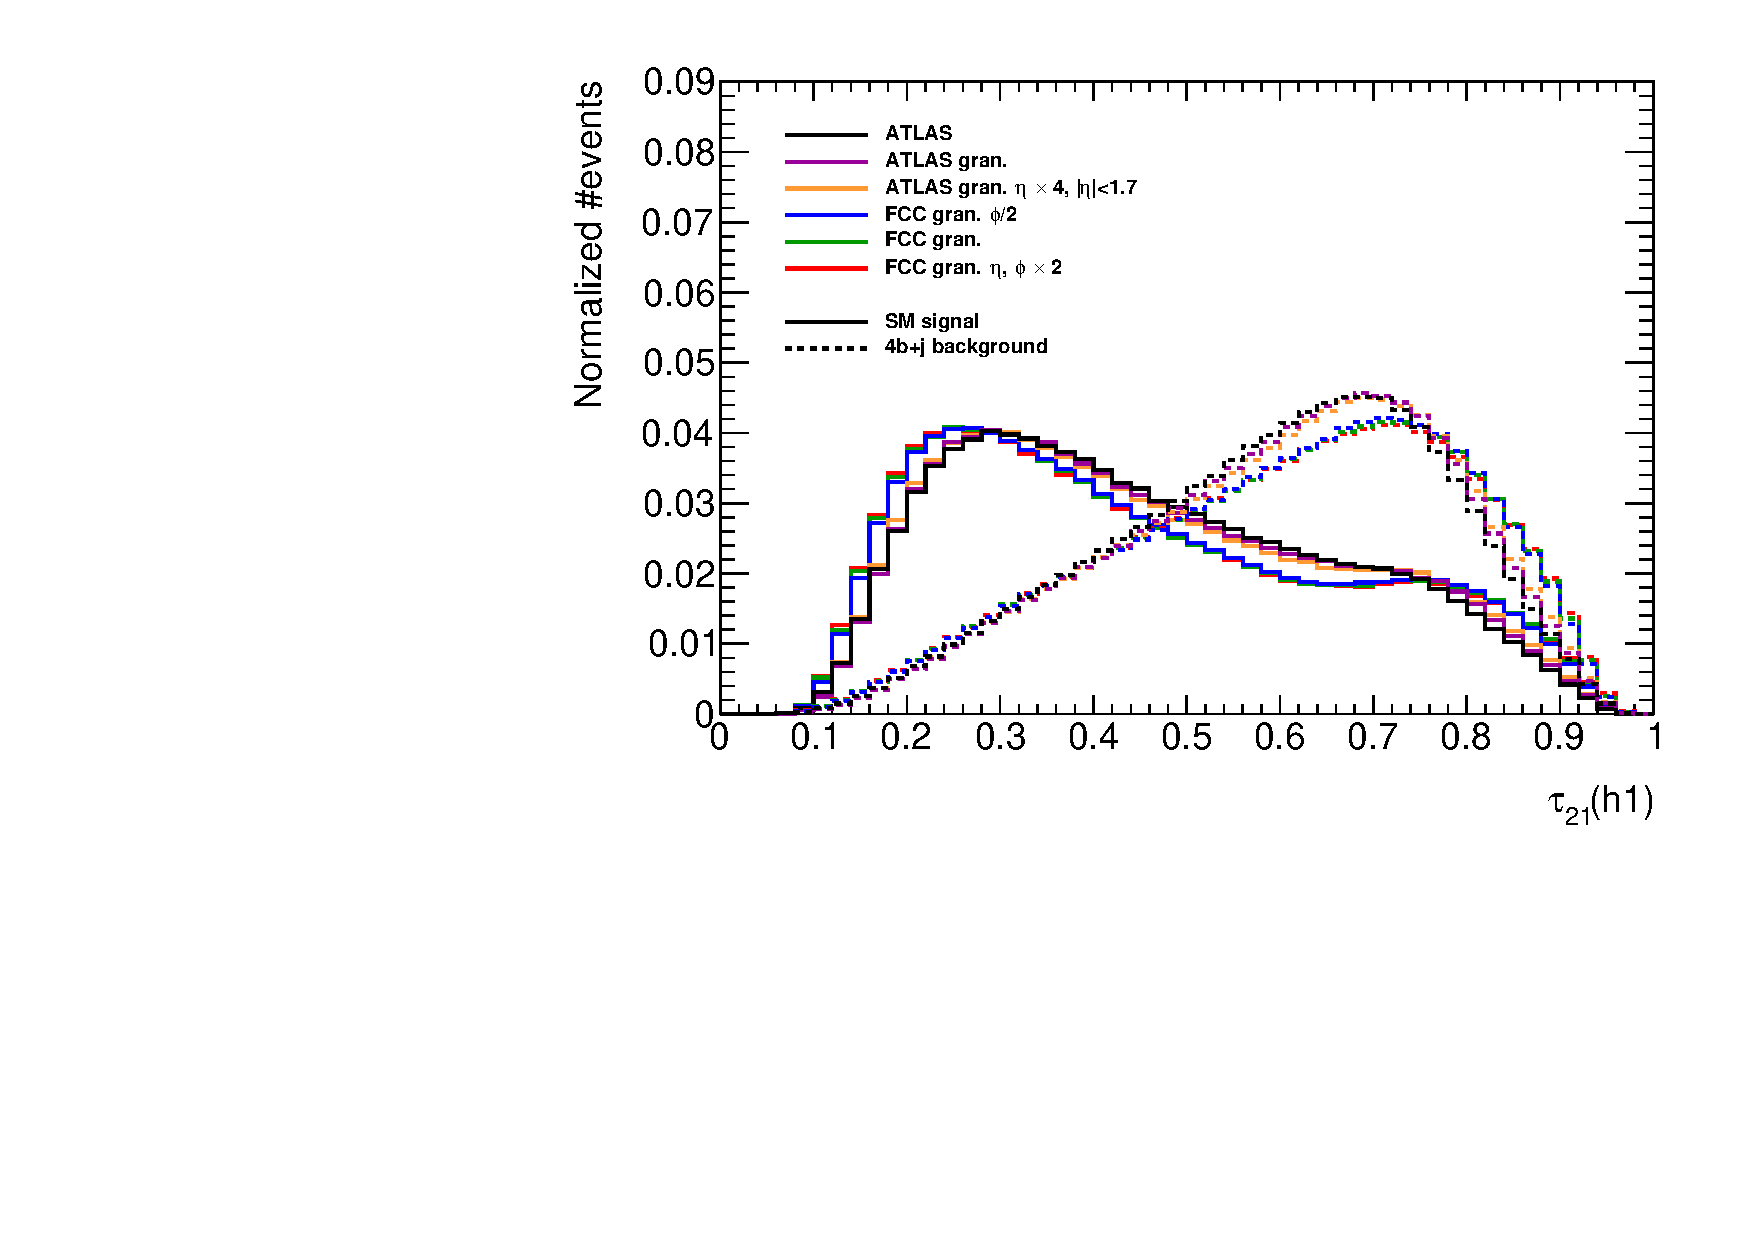
\includegraphics[trim={0 0 .65cm 0},clip,width=\linewidth]{./Figures/tau21.pdf}
		%\caption{Leading Higgs candidate $\tau_{21}$ plot for the different detector configurations for the SM signal sample. This plot contains all the signal events that passed all the cuts of the baseline analysis.}
		\label{fig:CompGran_tau21}
	\end{minipage}
	\label{fig:CompGran}
	\caption{Leading Higgs candidate softdrop mass (left) and $\tau_{21}$ (right) plots for the different detector configurations for the SM signal sample. The plots contain all the signal events that passed all the cuts of the baseline analysis. For the plot on the left note that the x axis range is from $80$ GeV to $160$ GeV in order to make the differences between the histograms more clear.}
\end{figure}

%\begin{figure}
%	\centering
%	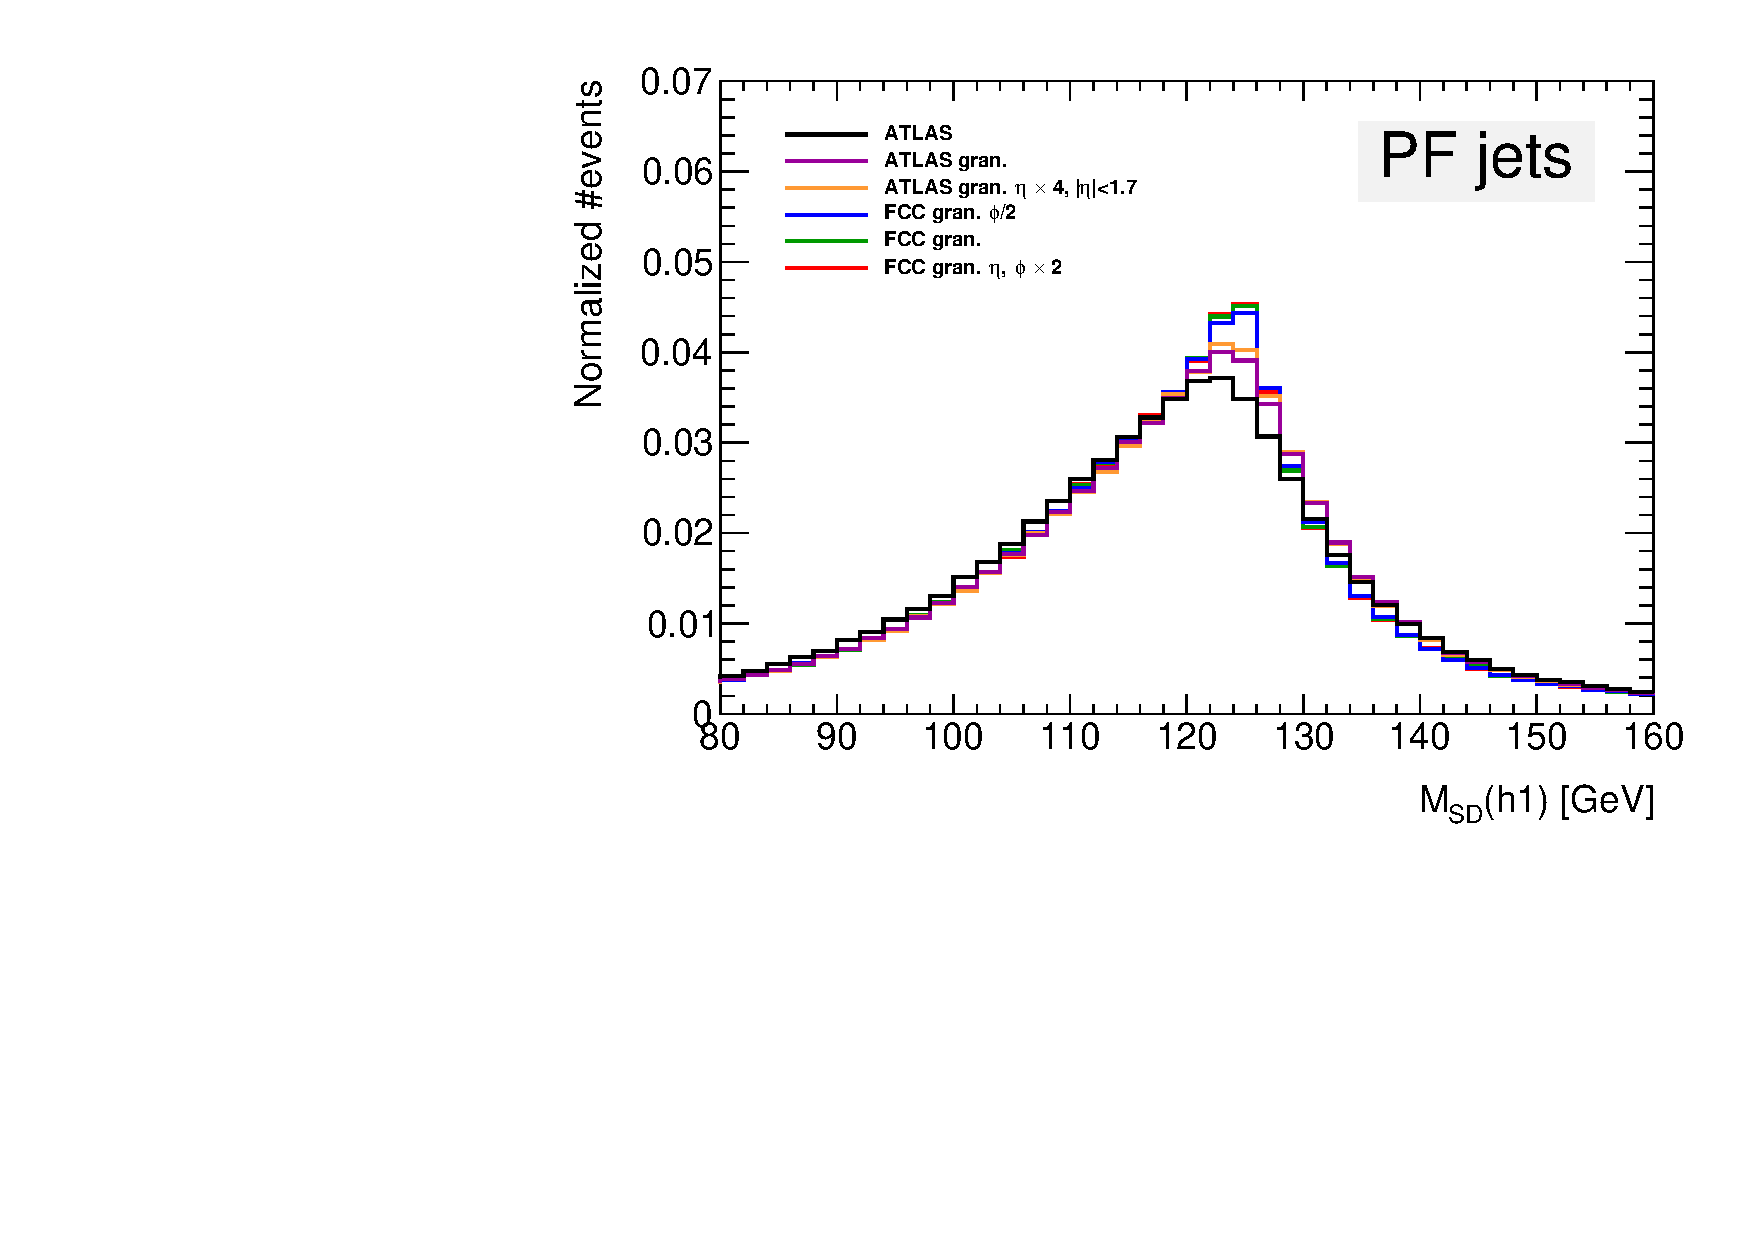
\includegraphics[width=\linewidth]{./Figures/M.pdf}
%	\label{fig:CompGran_M}
%	\caption{Leading Higgs candidate softdrop mass plot for the different detector configurations for the SM signal sample. This plot contains all the signal events that passed all the cuts of the baseline analysis. Note that the x axis range is from $80$ GeV to $160$ GeV in order to make the differences between the histograms more clear.}
%\end{figure}
%
%\begin{figure}
%	\centering
%	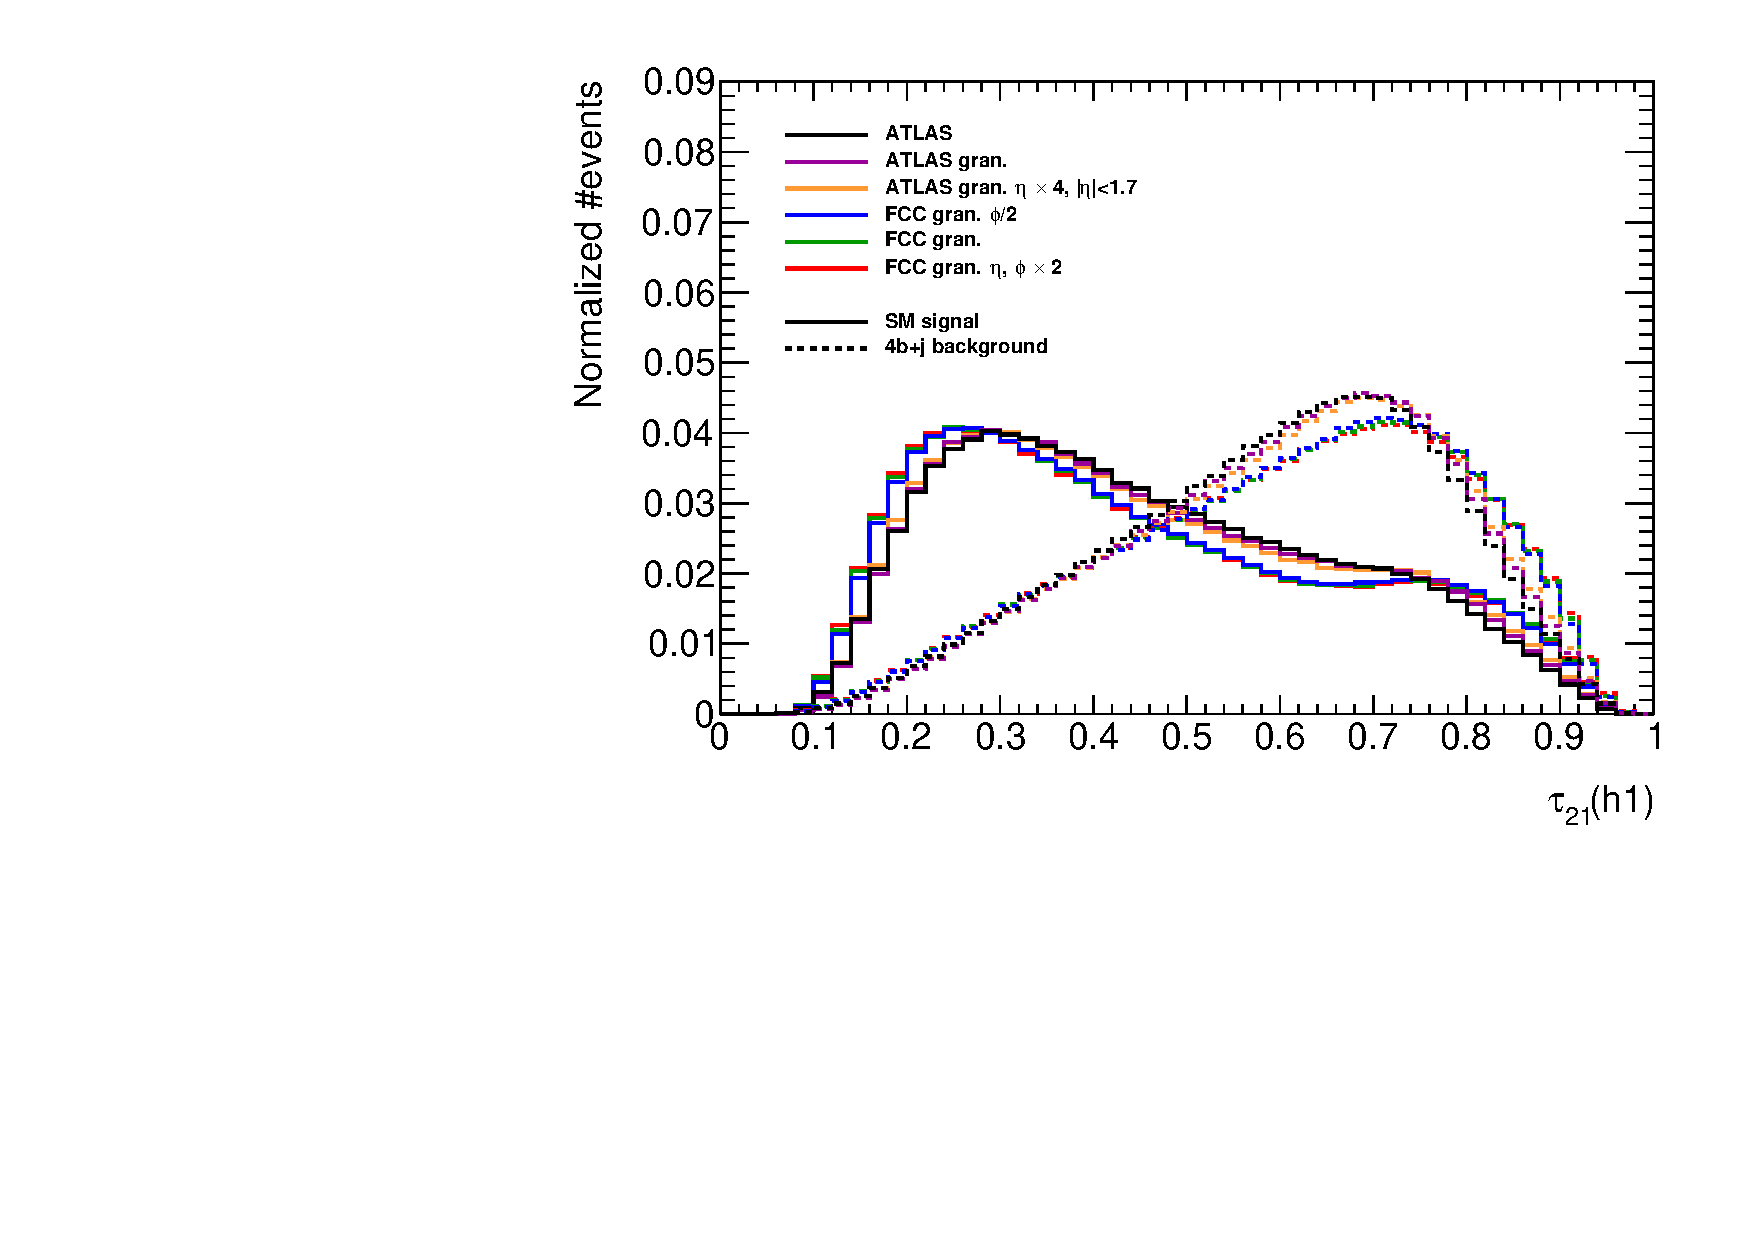
\includegraphics[width=\linewidth]{./Figures/tau21.pdf}
%	\label{fig:CompGran_tau21}
%	\caption{Leading Higgs candidate $\tau_{21}$ plot for the different detector configurations for the SM signal sample. This plot contains all the signal events that passed all the cuts of the baseline analysis.}
%\end{figure}

\begin{figure}
	\centering
	\begin{minipage}{.5\textwidth}
		\centering
		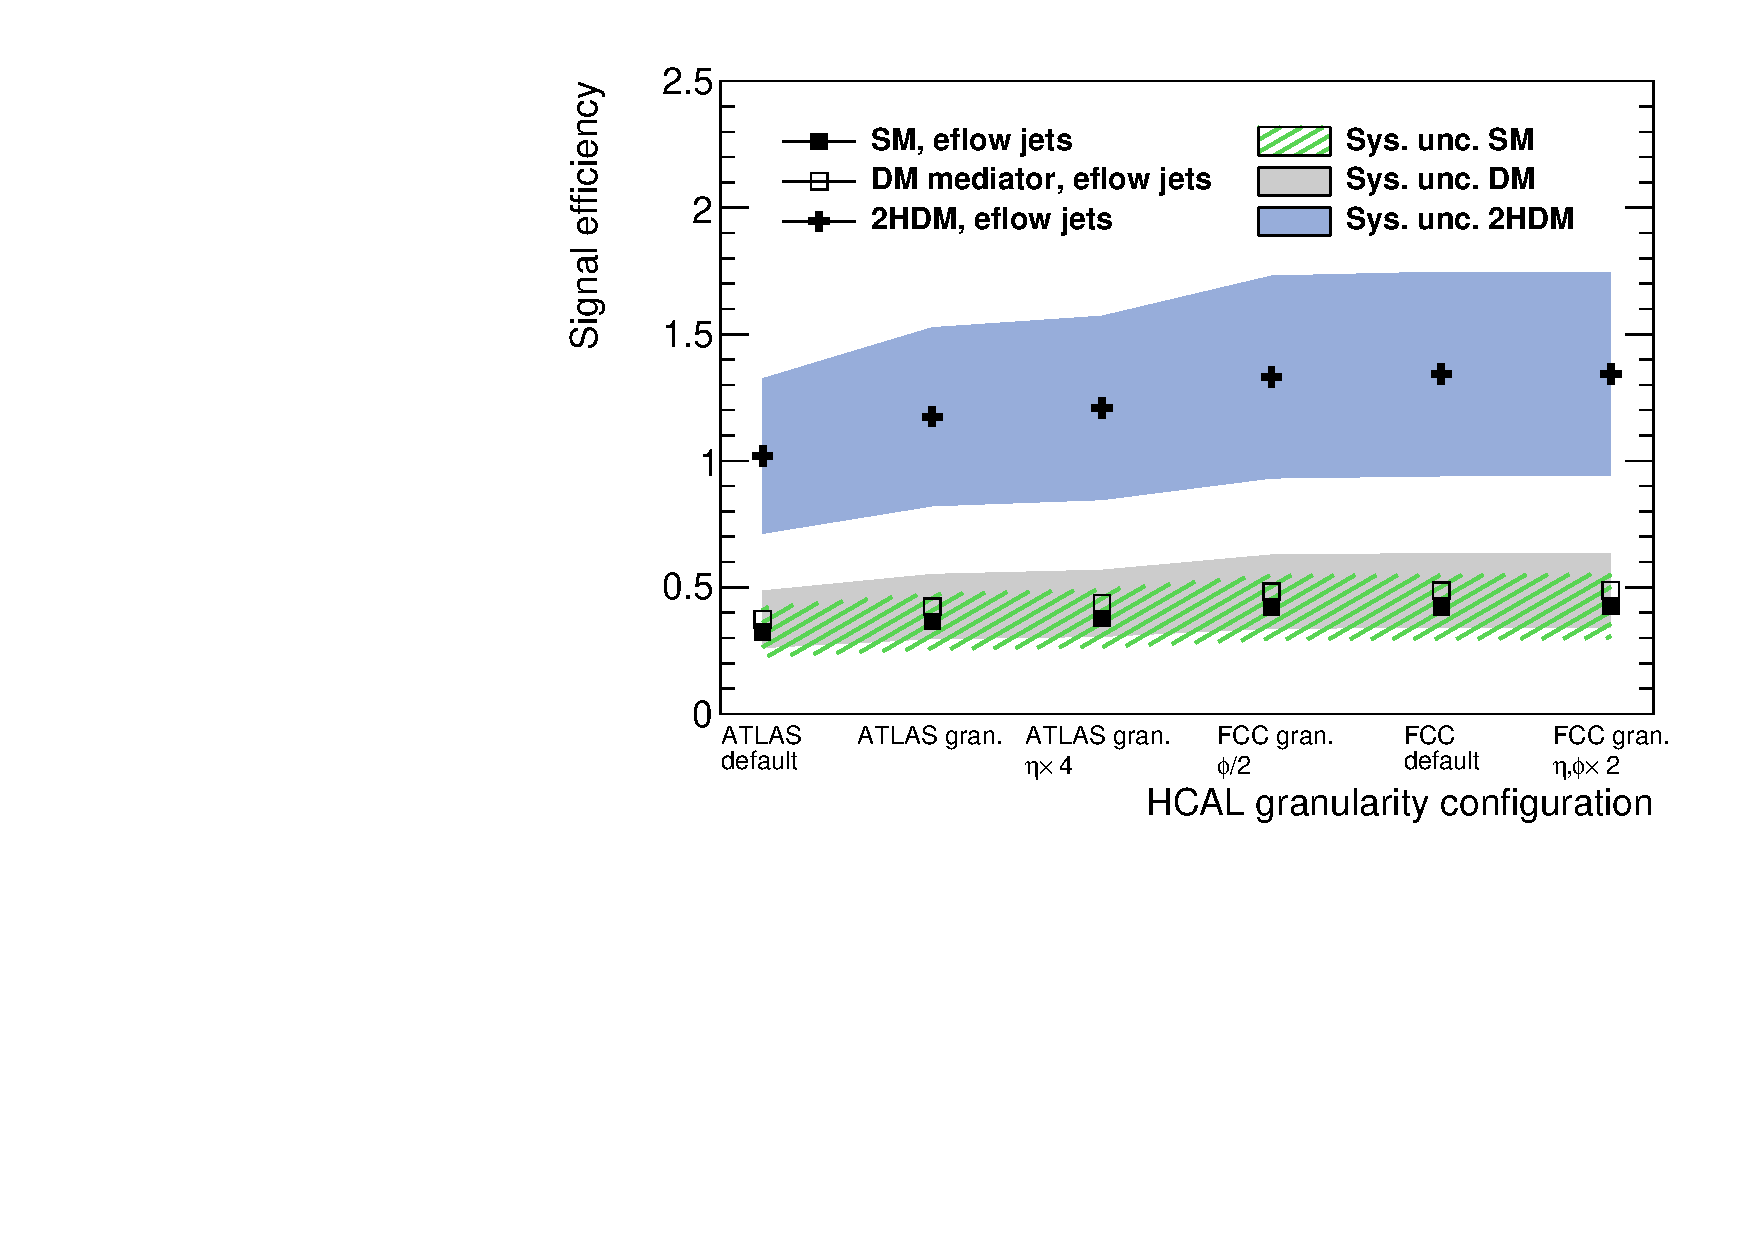
\includegraphics[trim={.6cm 0 0 0},clip,width=\linewidth]{./Figures/EffvsGran_PFjets.pdf}
	\end{minipage}%
	\begin{minipage}{.5\textwidth}
		\centering
		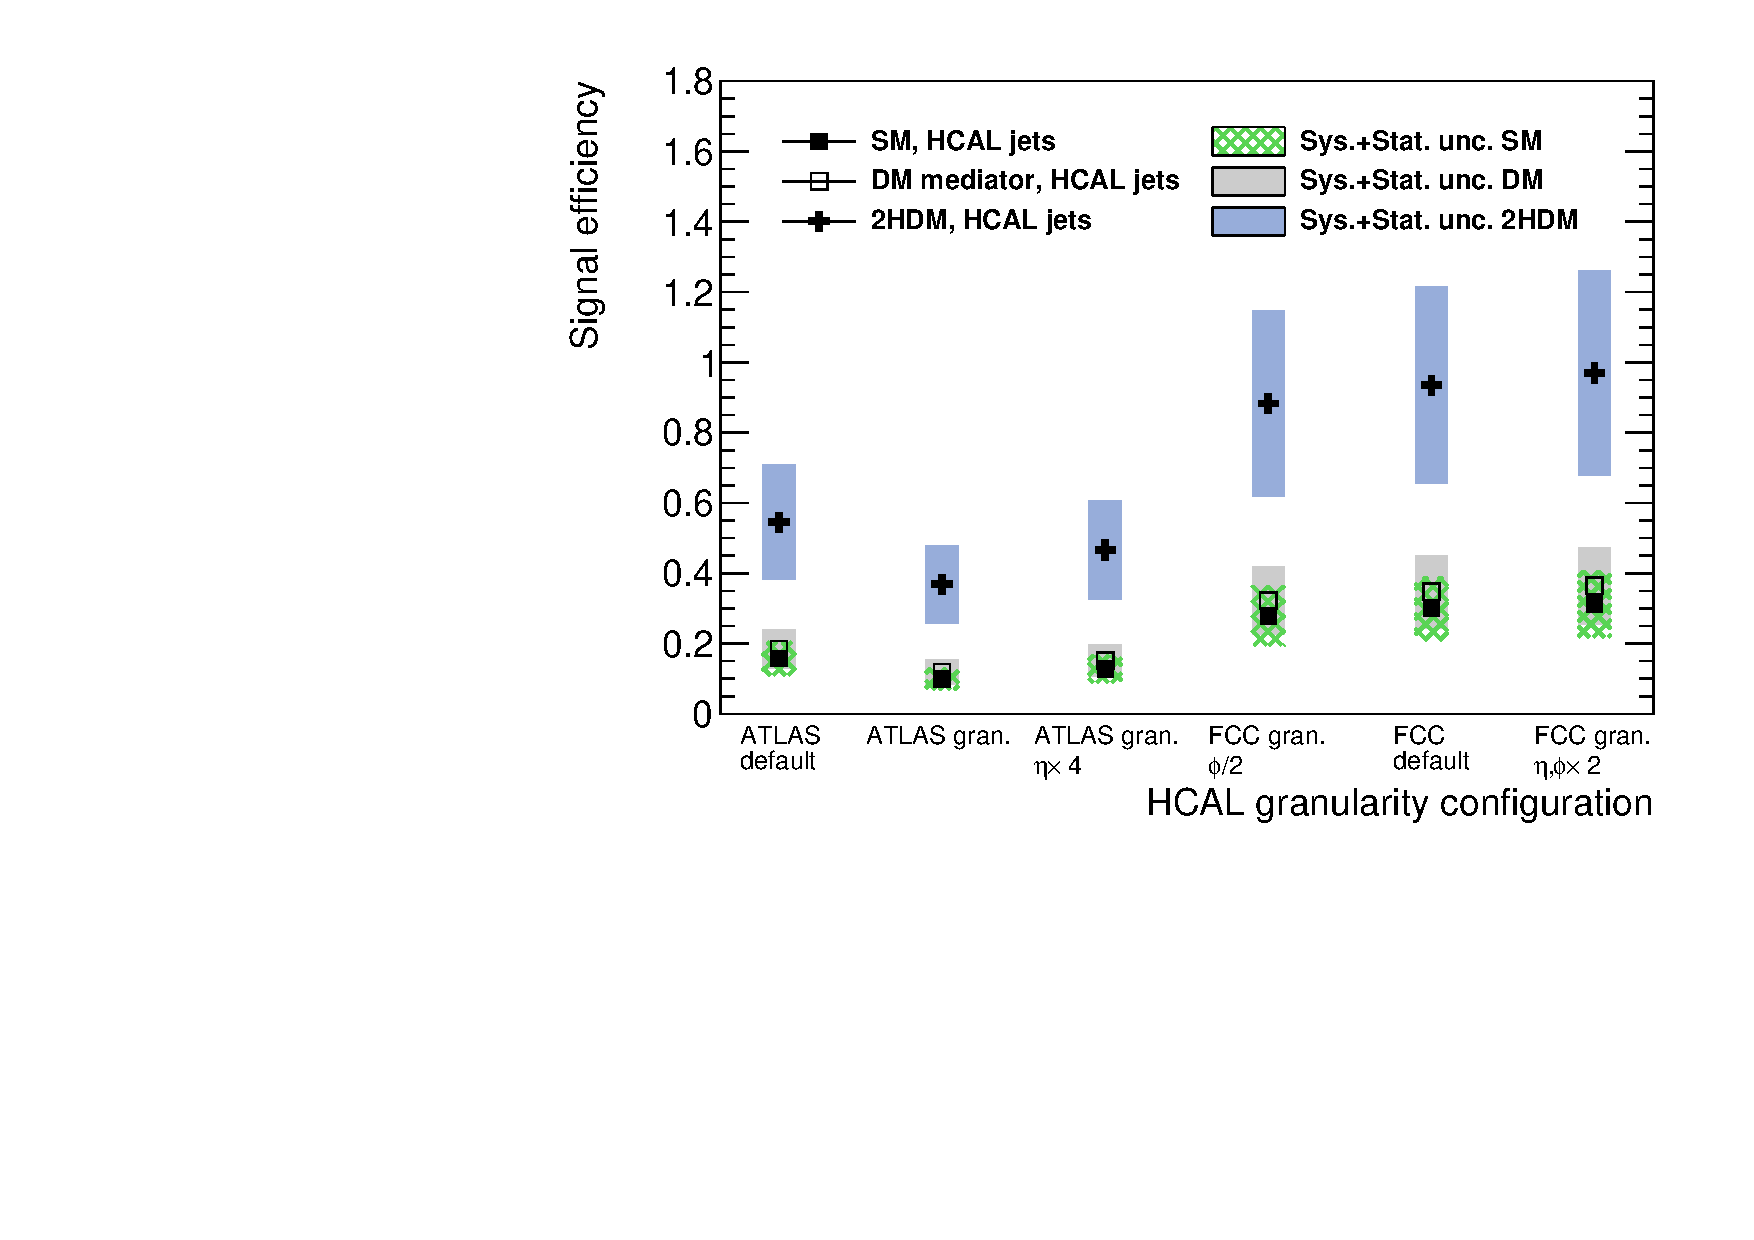
\includegraphics[trim={0 0 .6cm 0},clip,width=\linewidth]{./Figures/EffvsGran_CALOjets.pdf}
	\end{minipage}
	\label{fig:EffvsGran}
	\caption{Signal efficiency as a function of the detector configuration for particle flow jets (left) and pure calorimeter (HCAL) jets (right). Three signal models are shown: SM (filled squares), $1$ TeV DM mediator (empty squares) and type II 2HDM with $m_H=900$ GeV (crosses). The error bars are drawn but are smaller than the markers.}
\end{figure}

\begin{figure}
	\centering
	\begin{minipage}{.5\textwidth}
		\centering
		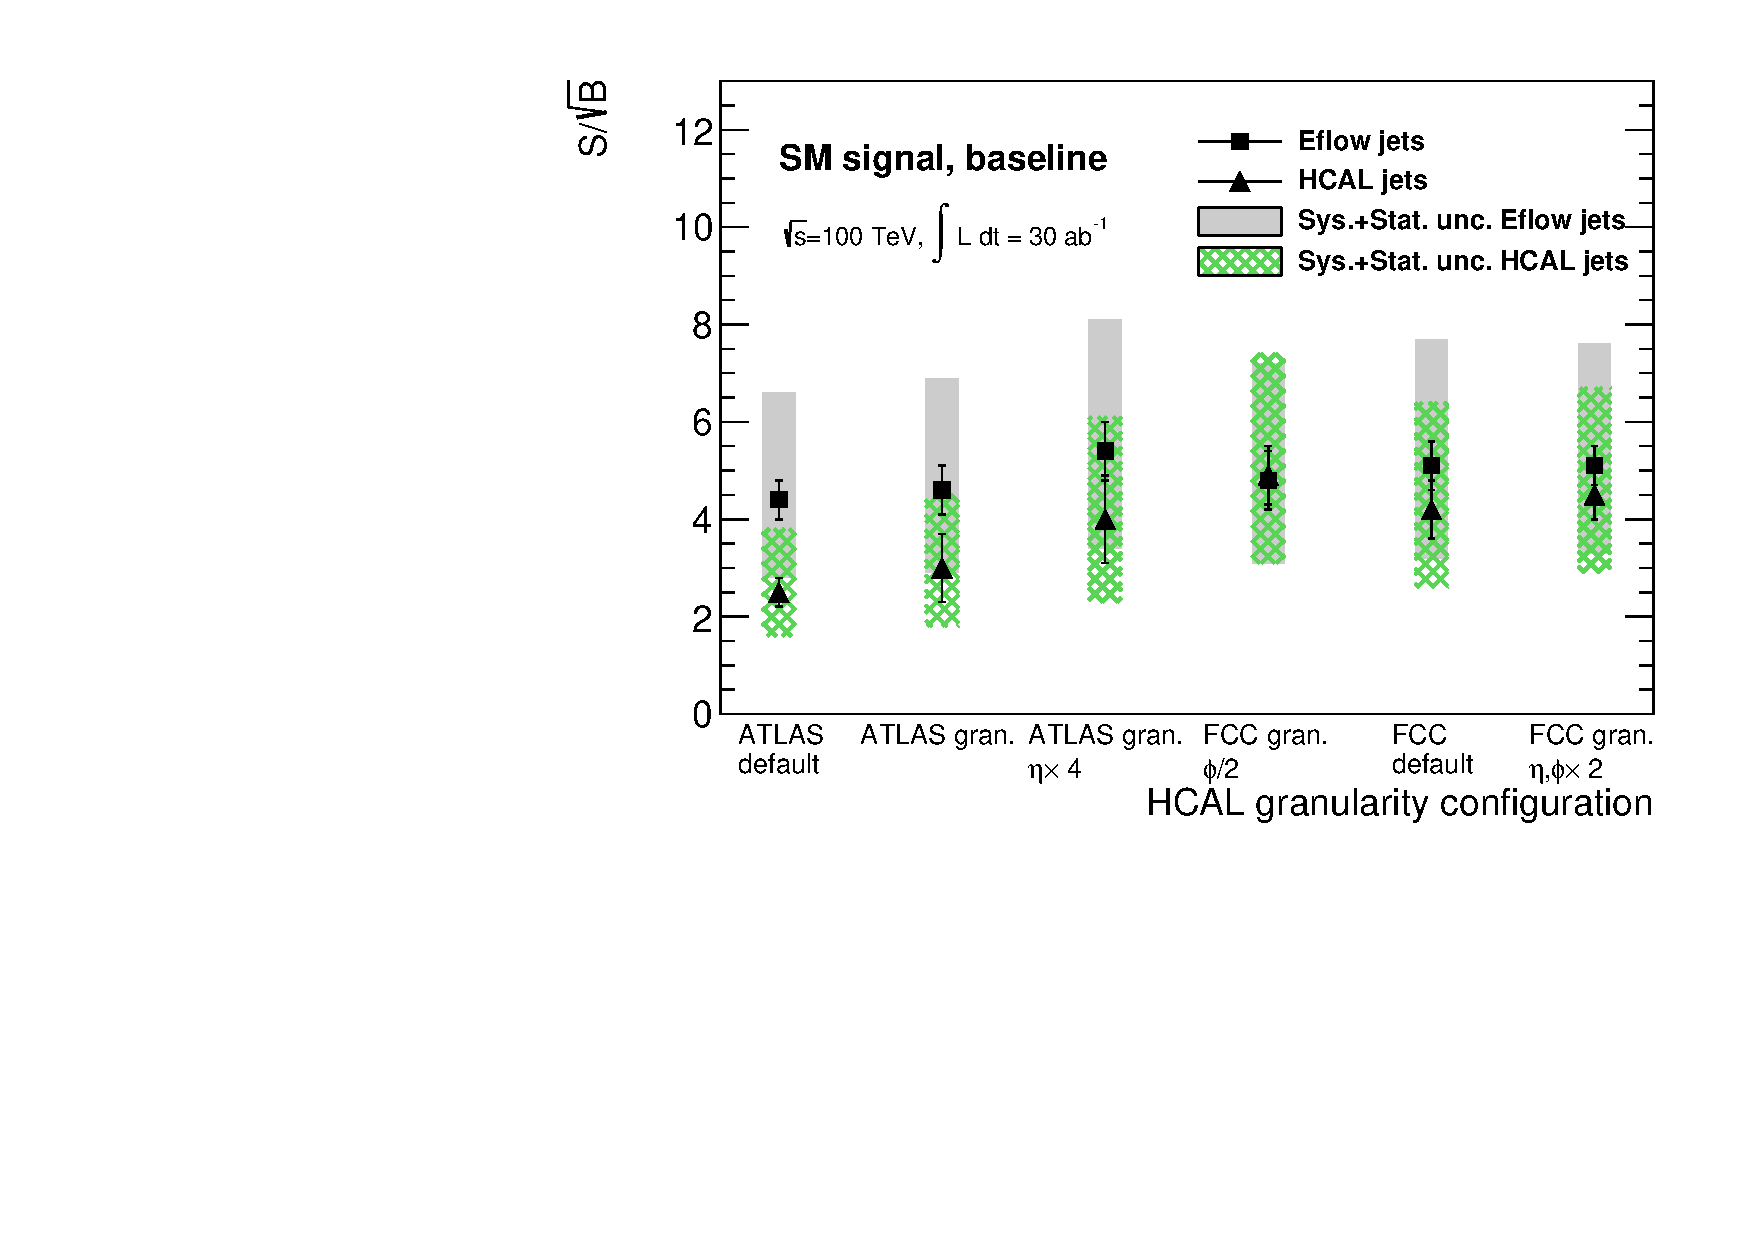
\includegraphics[trim={.6cm 0 0 0},clip,width=\linewidth]{./Figures/SSBvsGran_SM.pdf}
	\end{minipage}%
	\begin{minipage}{.5\textwidth}
		\centering
		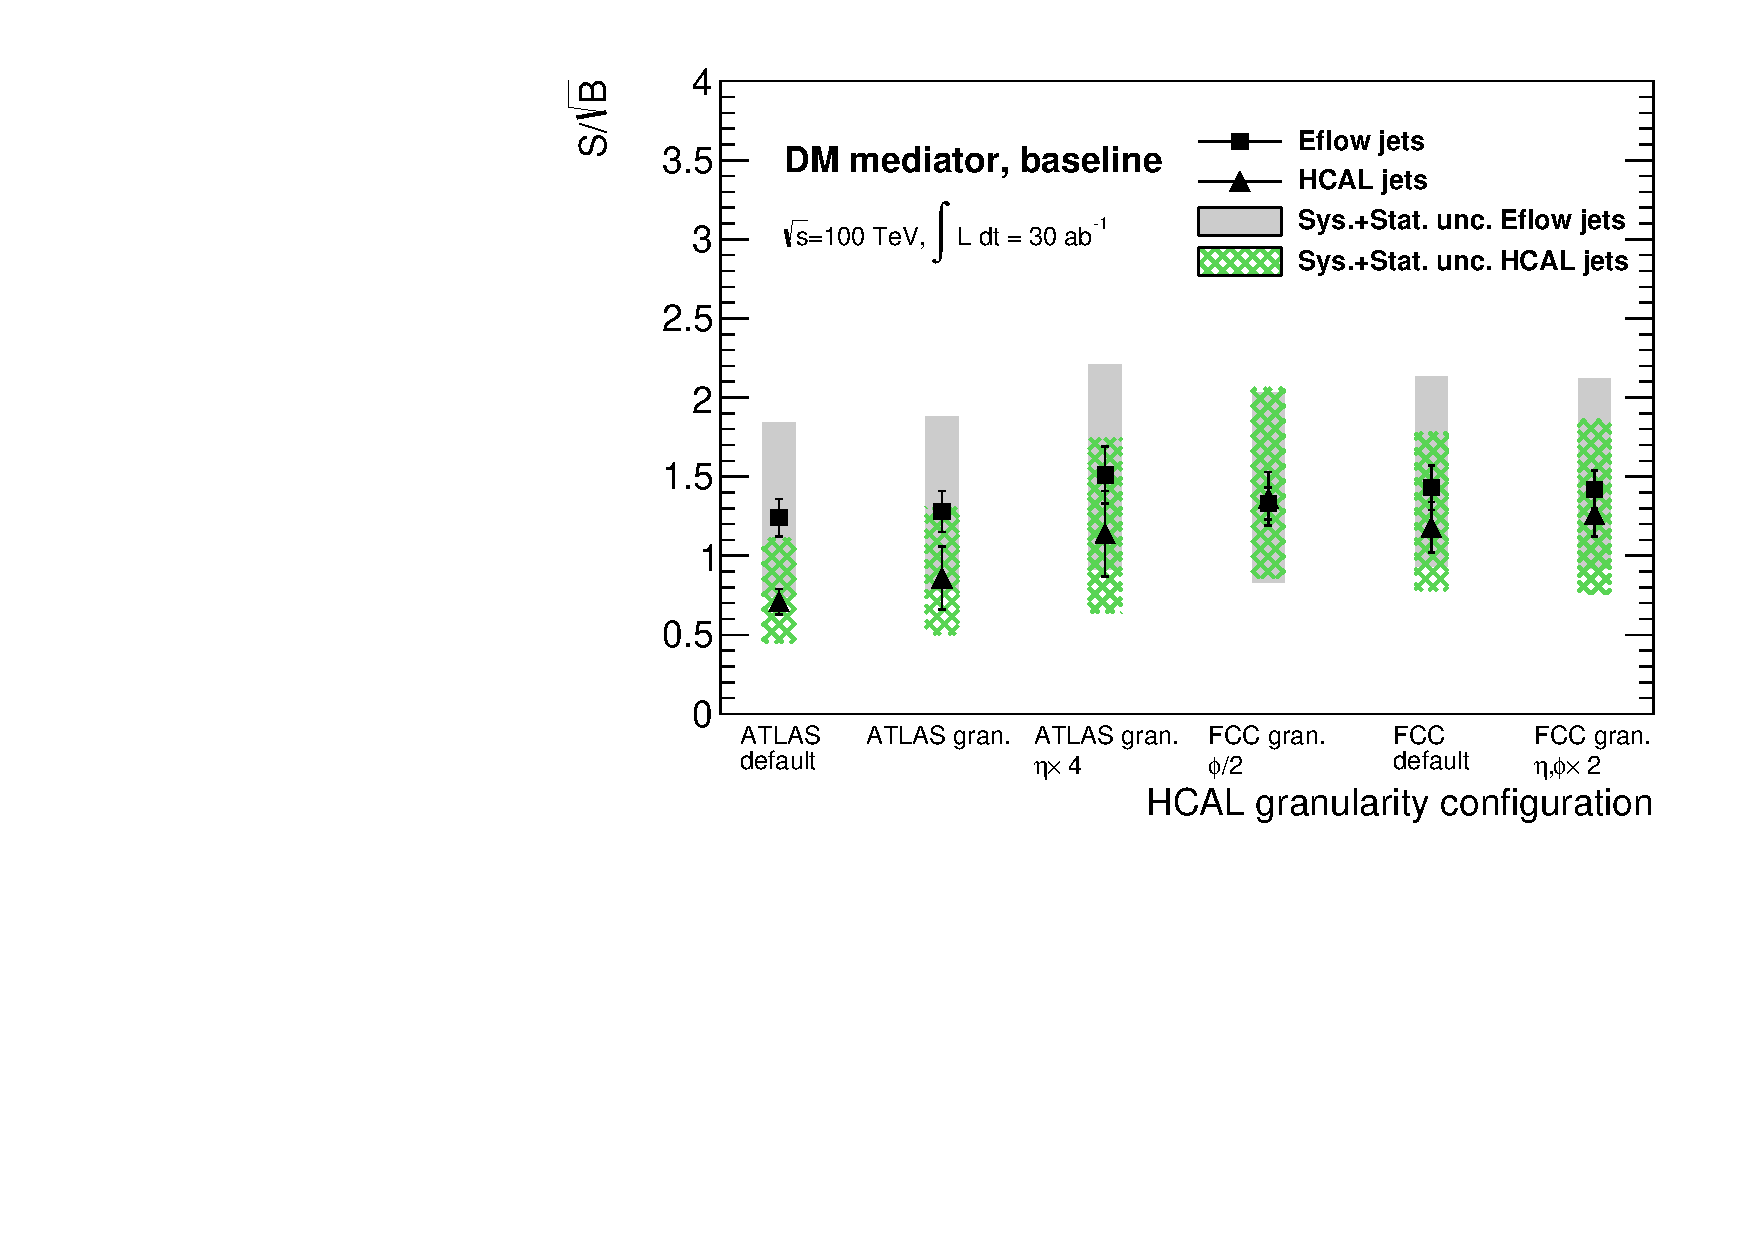
\includegraphics[trim={0 0 .6cm 0},clip,width=\linewidth]{./Figures/SSBvsGran_DM.pdf}
	\end{minipage}
	\label{fig:SSBvsGran1}
	\caption{Significance $(S/\sqrt{B})$ as a function of the detector configuration for $\mathcal{L}=30~\text{ab}^{-1}$ (filled) and $\mathcal{L}=3~\text{ab}^{-1}$ (empty) and for particle flow jets (squares) and pure calorimeter (HCAL) jets (triangles) for the SM signal model (left) and for the $1$ TeV DM mediator model (right).}
\end{figure}

\begin{figure}
	\centering
	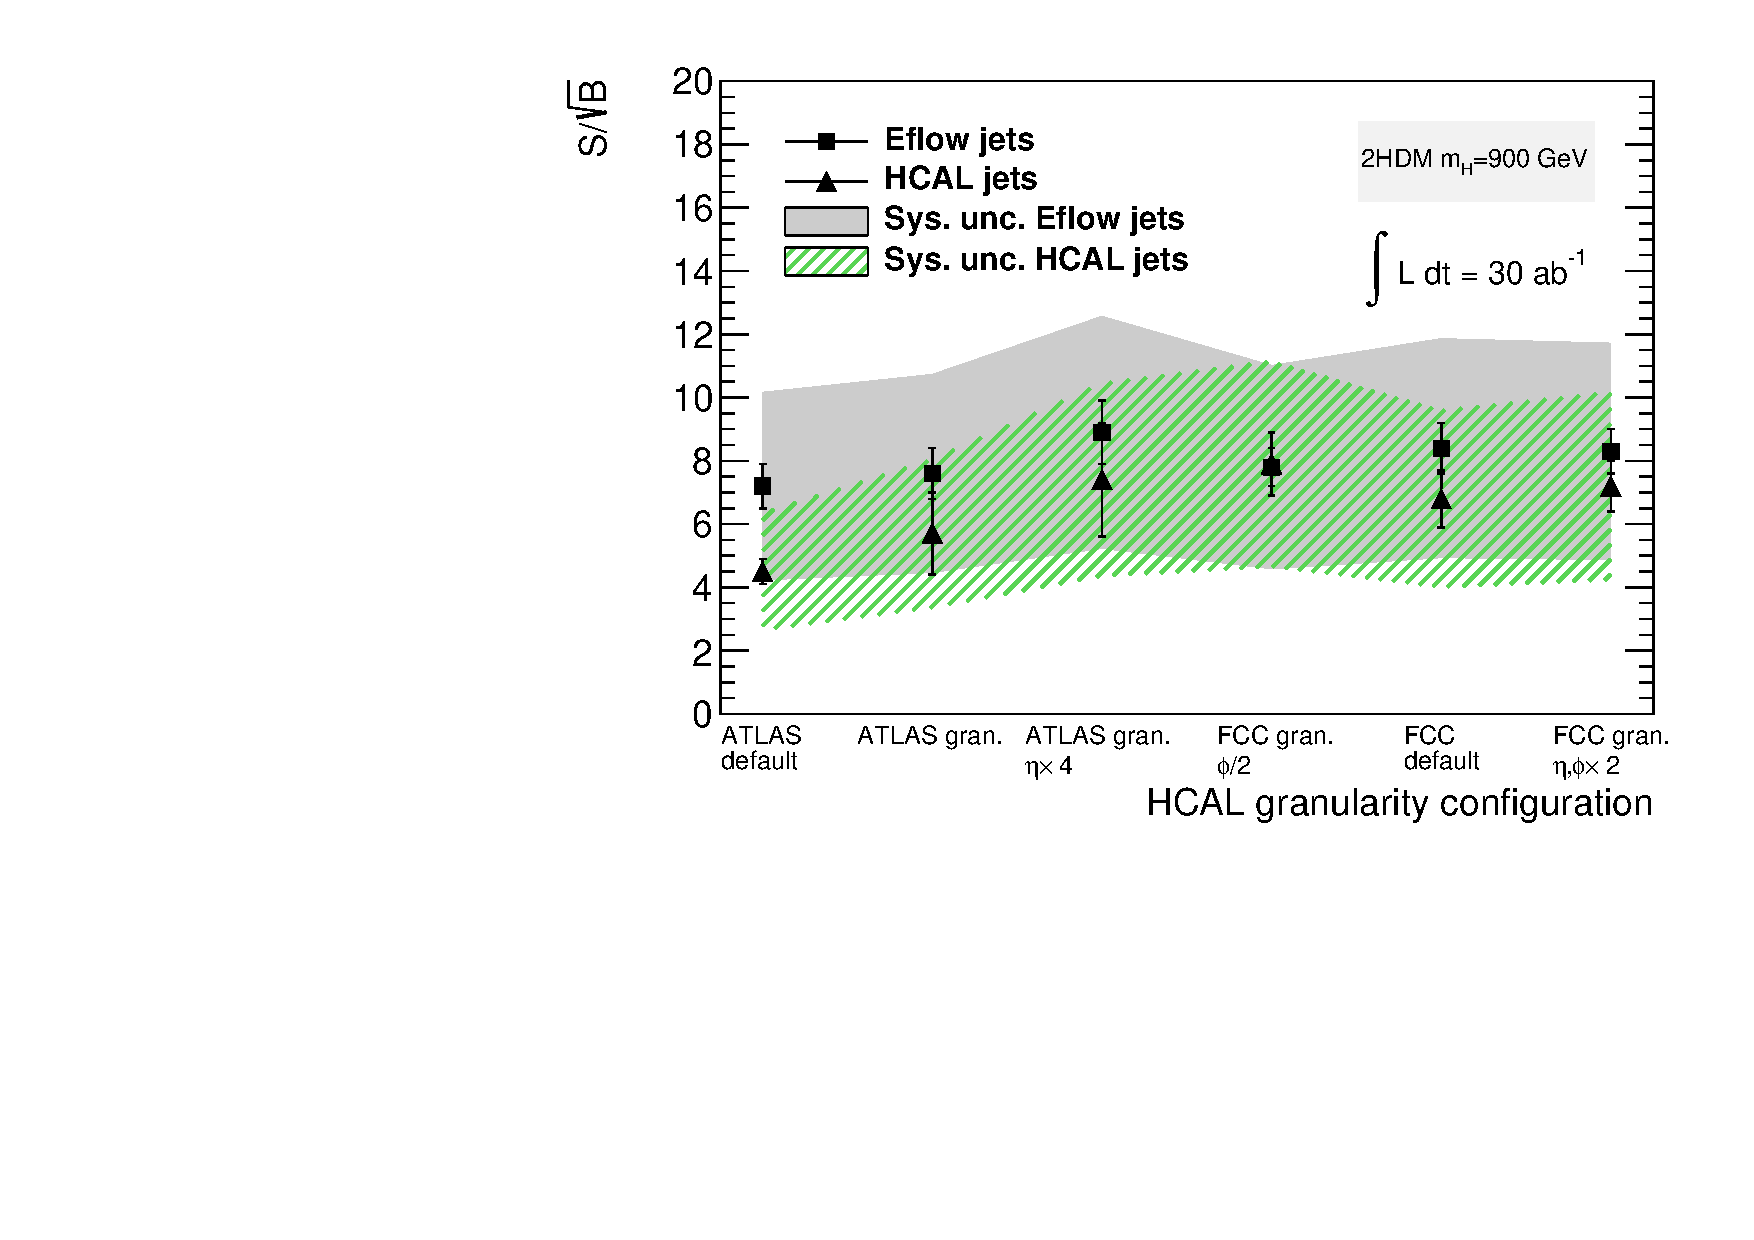
\includegraphics[width=0.5\linewidth]{./Figures/SSBvsGran_2HDM.pdf}
	\label{fig:SSBvsGran_2HDM}
	\caption{Significance $(S/\sqrt{B})$ as a function of the detector configuration for $\mathcal{L}=30~\text{ab}^{-1}$ (filled) and $\mathcal{L}=3~\text{ab}^{-1}$ (empty) and for particle flow jets (squares) and pure calorimeter (HCAL) jets (triangles) for the type II 2HDM with $m_H=900$ GeV.}
\end{figure}

%\begin{figure}[!htb]
%  \centering
%  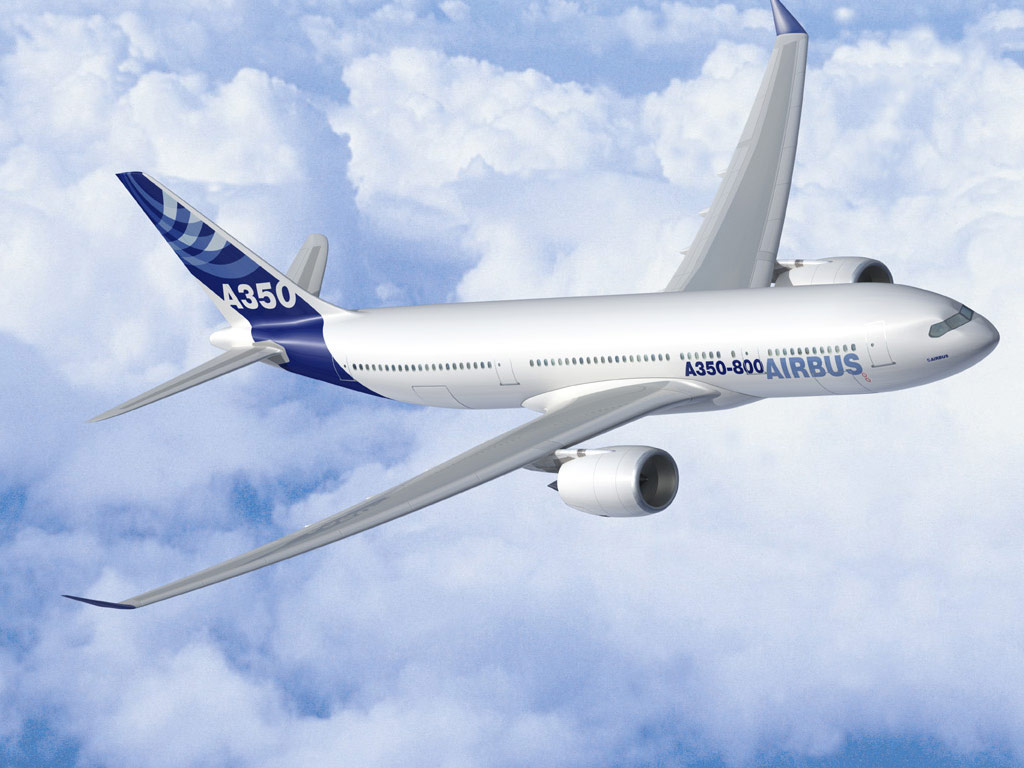
\includegraphics[width=0.25\textwidth]{Figures/Airbus_A350.jpg}
%  \caption[Caption for figure in TOC.]{Caption for figure.}
%  \label{fig:airbus1}
%\end{figure}
%
%\begin{figure}[!htb]
%  \begin{subfigmatrix}{2}
%    \subfigure[Airbus A320]{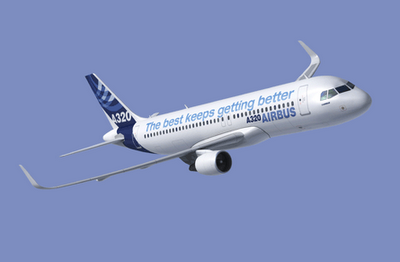
\includegraphics[width=0.49\linewidth]{Figures/Airbus_A320_sharklets.png}}
%    \subfigure[Bombardier CRJ200]{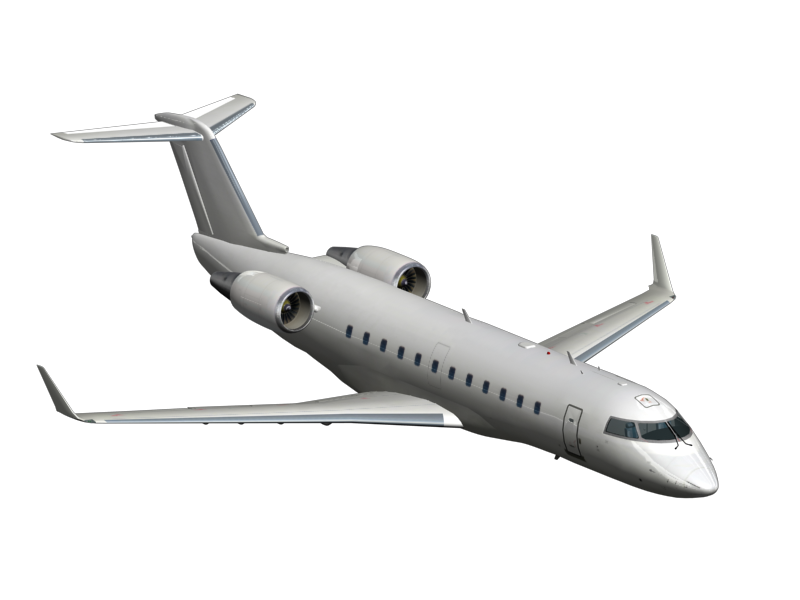
\includegraphics[width=0.49\linewidth]{Figures/Bombardier_CRJ200.png}}
%  \end{subfigmatrix}
%  \caption{Some aircrafts.}
%  \label{fig:aircrafts}
%\end{figure}
%
%Make reference to Figures \ref{fig:airbus1} and \ref{fig:aircrafts}.
%
%By default, the supported file types are {\it .png,.pdf,.jpg,.mps,.jpeg,.PNG,.PDF,.JPG,.JPEG}.
%
%See \url{http://mactex-wiki.tug.org/wiki/index.php/Graphics_inclusion} for adding support to other extensions.
%
%
%% ----------------------------------------------------------------------
%\subsubsection{Drawings}
%\label{subsection:drawings}
%
%Insert your subsection material and for instance a few drawings...
%
%The schematic illustrated in Fig.~\ref{fig:algorithm} can represent some sort of algorithm.
%
%\begin{figure}[!htb]
%  \centering
%  \scriptsize
%%  \footnotesize 
%%  \small
%  \setlength{\unitlength}{0.9cm}
%  \begin{picture}(8.5,6)
%    \linethickness{0.3mm}
%
%    \put(3,6){\vector(0,-1){1}}
%    \put(3.5,5.4){$\bf \alpha$}
%    \put(3,4.5){\oval(6,1){}}
%    %\put(0,4){\framebox(6,1){}}
%    \put(0.3,4.4){Grid Generation: \quad ${\bf x} = {\bf x}\left({\bf \alpha}\right)$}
%
%    \put(3,4){\vector(0,-1){1}}
%    \put(3.5,3.4){$\bf x$}
%    \put(3,2.5){\oval(6,1){}}
%    %\put(0,2){\framebox(6,1){}}
%    \put(0.3,2.4){Flow Solver: \quad ${\cal R}\left({\bf x},{\bf q}\left({\bf x}\right)\right) = 0$}
%
%    \put(6.0,2.5){\vector(1,0){1}}
%    \put(6.4,3){$Y_1$}
%
%    \put(3,2){\vector(0,-1){1}}
%    \put(3.5,1.4){$\bf q$}
%    \put(3,0.5){\oval(6,1){}}
%    %\put(0,0){\framebox(6,1){}}
%    \put(0.3,0.4){Structural Solver: \quad ${\cal M}\left({\bf x},{\bf q}\left({\bf x}\right)\right) = 0$}
%
%    \put(6.0,0.5){\vector(1,0){1}}
%    \put(6.4,1){$Y_2$}
%
%    %\put(7.8,2.5){\oval(1.6,5){}}
%    \put(7.0,0){\framebox(1.6,5){}}
%    \put(7.1,2.5){Optimizer}
%    \put(7.8,5){\line(0,1){1}}
%    \put(7.8,6){\line(-1,0){4.8}}
%  \end{picture}
%  \caption{Schematic of some algorithm.}
%  \label{fig:algorithm}
%\end{figure}
%
%
%% ----------------------------------------------------------------------
%\subsection{Equations}
%\label{subsection:equations}
%
%Equations can be inserted in different ways.
%
%The simplest way is in a separate line like this
%
%\begin{equation}
%  \frac{{\rm d} q_{ijk}}{{\rm d} t} + {\cal R}_{ijk}({\bf q}) = 0 \,.
%\label{eq:ode}
%\end{equation}
%
%If the equation is to be embedded in the text. One can do it like this ${\partial {\cal R}}/{\partial {\bf q}}=0$.
%
%It may also be split in different lines like this
%
%\begin{eqnarray}
%  {\rm Minimize}   && Y({\bf \alpha},{\bf q}({\bf \alpha}))            \nonumber           \\
%  {\rm w.r.t.}     && {\bf \alpha} \,,                                 \label{eq:minimize} \\
%  {\rm subject~to} && {\cal R}({\bf \alpha},{\bf q}({\bf \alpha})) = 0 \nonumber           \\
%                   &&       C ({\bf \alpha},{\bf q}({\bf \alpha})) = 0 \,. \nonumber
%\end{eqnarray}
%
%It is also possible to use subequations. Equations~\ref{eq:continuity}, \ref{eq:momentum} and \ref{eq:energy} form the Naver--Stokes equations~\ref{eq:NavierStokes}.
%
%\begin{subequations}
%    \begin{equation}
%    \frac{\partial \rho}{\partial t} + \frac{\partial}{\partial x_j}\left( \rho u_j \right) = 0 \,,
%    \label{eq:continuity}
%    \end{equation}
%    \begin{equation}
%    \frac{\partial}{\partial t}\left( \rho u_i \right) + \frac{\partial}{\partial x_j} \left( \rho u_i u_j + p \delta_{ij} - \tau_{ji} \right) = 0, \quad i=1,2,3 \,,
%    \label{eq:momentum}
%    \end{equation}
%    \begin{equation}
%        \frac{\partial}{\partial t}\left( \rho E \right) + \frac{\partial}{\partial x_j} \left( \rho E u_j + p u_j - u_i \tau_{ij} + q_j \right) = 0 \,.
%    \label{eq:energy}
%    \end{equation}
%\label{eq:NavierStokes}%
%\end{subequations}
%
%
%% ----------------------------------------------------------------------
%\subsection{Tables}
%\label{section:tables}
%
%Insert your subsection material and for instance a few tables...
%
%Make sure all tables presented are referenced in the text!
%
%Follow some guidelines when making tables:
%
%\begin{itemize}
%  \item Avoid vertical lines
%  \item Avoid “boxing up” cells, usually 3 horizontal lines are enough: above, below, and after heading
%  \item Avoid double horizontal lines
%  \item Add enough space between rows
%\end{itemize}
%
%\begin{table}[!htb]
%  \renewcommand{\arraystretch}{1.2} % more space between rows
%  \centering
%  \begin{tabular}{lccc}
%    \toprule
%    Model           & $C_L$ & $C_D$ & $C_{M y}$ \\
%    \midrule
%    Euler           & 0.083 & 0.021 & -0.110    \\
%    Navier--Stokes  & 0.078 & 0.023 & -0.101    \\
%    \bottomrule
%  \end{tabular}
%  \caption[Table caption shown in TOC.]{Table caption.}
%  \label{tab:aeroCoeff}
%\end{table}
%
%Make reference to Table \ref{tab:aeroCoeff}.
%
%Tables \ref{tab:memory} and \ref{tab:multipleColumns} are examples of tables with merging columns:
%
%\begin{table}[!htb]
%  \renewcommand{\arraystretch}{1.2} % more space between rows
%  \centering
%  \begin{tabular}[]{lrr}
%    \toprule
%                & \multicolumn{2}{c}{\underline{Virtual memory [MB]}} \\
%                & Euler       & Navier--Stokes \\
%    \midrule
%      Wing only &  1,000      &    2,000       \\
%      Aircraft  &  5,000      &   10,000       \\
%      (ratio)   & $5.0\times$ & $5.0\times$    \\
%    \bottomrule
%  \end{tabular}
%  \caption{Memory usage comparison (in MB).}
%  \label{tab:memory}
%\end{table}
%
%\begin{table}[!htb]
%  \centering
%  \renewcommand{\arraystretch}{1.2} % more space between rows
%  \begin{tabular}{@{}rrrrcrrr@{}} % remove space to the vertical edges @{}...@{}
%    \toprule
%      & \multicolumn{3}{c}{$w = 2$} & \phantom{abc} & \multicolumn{3}{c}{$w = 4$} \\
%    \cmidrule{2-4}
%    \cmidrule{6-8}
%      & $t=0$ & $t=1$ & $t=2$ && $t=0$ & $t=1$ & $t=2$ \\
%    \midrule
%      $dir=1$
%      \\
%      $c$ &  0.07 &  0.16 &  0.29 &&  0.36 &  0.71 &   3.18 \\
%      $c$ & -0.86 & 50.04 &  5.93 && -9.07 & 29.09 &  46.21 \\
%      $c$ & 14.27 &-50.96 &-14.27 && 12.22 &-63.54 &-381.09 \\
%      $dir=0$
%      \\
%      $c$ &  0.03 &  1.24 &  0.21 &&  0.35 & -0.27 &  2.14 \\
%      $c$ &-17.90 &-37.11 &  8.85 &&-30.73 & -9.59 & -3.00 \\
%      $c$ &105.55 & 23.11 &-94.73 &&100.24 & 41.27 &-25.73 \\
%    \bottomrule
%  \end{tabular}
%  \caption{Another table caption.}
%  \label{tab:multipleColumns}
%\end{table}
%
%An example with merging rows can be seen in Tab.\ref{tab:multipleRows}.
%
%\begin{table}[!htb]
%  \renewcommand{\arraystretch}{1.2} % more space between rows
%  \centering
%  \begin{tabular}{ccccc}
%    \toprule
%      \multirow{2}{*}{ABC} & \multicolumn{4}{c}{header} \\
%      \cmidrule{2-5} & 1.1 & 2.2 & 3.3 & 4.4 \\
%    \midrule
%      \multirow{2}{*}{IJK} & \multicolumn{2}{c}{\multirow{2}{*}{group}} & 0.5 & 0.6 \\
%      \cmidrule{4-5}       & \multicolumn{2}{c}{}                       & 0.7 & 1.2 \\
%    \bottomrule
%  \end{tabular}
%  \caption{Yet another table caption.}
%  \label{tab:multipleRows}
%\end{table}
%
%If the table has too many columns, it can be scaled to fit the text widht, as in Tab.\ref{tab:scale}.
%\begin{table}[!htb]
%  \renewcommand{\arraystretch}{1.2} % more space between rows
%  \centering
%  \resizebox*{\textwidth}{!}{%
%    \begin{tabular}[]{lcccccccccc}
%      \toprule
%        Variable &  a  &  b  &  c  &  d  &  e  &  f  &  g  &  h  &  i  &  j  \\
%      \midrule
%        Test 1   &  10,000 &  20,000 &  30,000 &  40,000 &  50,000 &  60,000 &  70,000 &  80,000 &  90,000 & 100,000 \\
%        Test 2   &  20,000 &  40,000 &  60,000 &  80,000 & 100,000 & 120,000 & 140,000 & 160,000 & 180,000 & 200,000 \\
%      \bottomrule
%    \end{tabular}
%  }%
%  \caption{Very wide table.}
%  \label{tab:scale}%
%\end{table}
%
%
%% ----------------------------------------------------------------------
%\subsection{Mixing}
%\label{section:mixing}
%
%If necessary, a figure and a table can be put side-by-side as in Fig.\ref{fig:side_by_side}
%
%\begin{figure}[!htb]
%  \begin{minipage}[b]{0.60\linewidth}
%    \centering
%    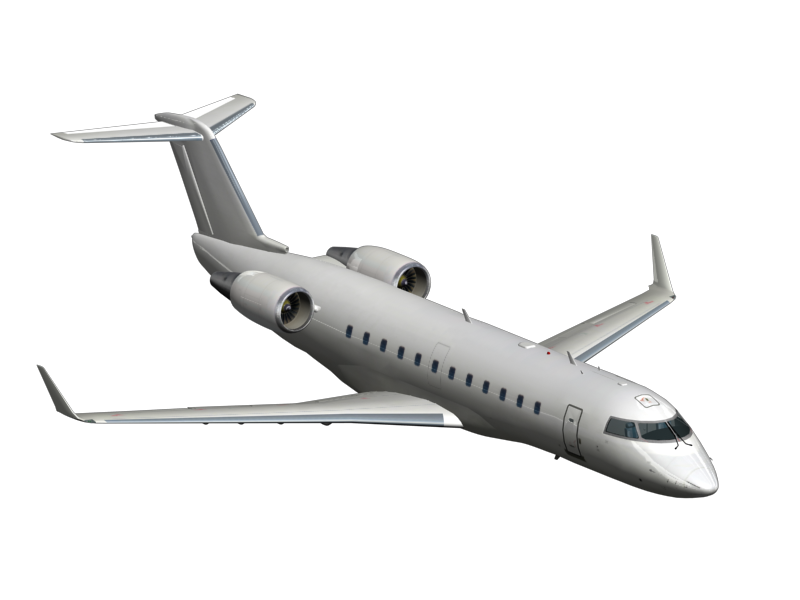
\includegraphics[width=\linewidth]{Figures/Bombardier_CRJ200}
%  \end{minipage}%
%  \begin{minipage}[b]{0.30\linewidth}
%    \centering
%    \begin{tabular}[b]{lll}
%      \toprule
%        \multicolumn{3}{c}{Legend} \\
%      \midrule
%        A & B & C \\
%        0 & 0 & 0 \\
%        0 & 1 & 0 \\
%        1 & 0 & 0 \\
%        1 & 1 & 1 \\
%      \bottomrule
%    \end{tabular}
%    \vspace{5em}
%  \end{minipage}
%\caption{Figure and table side-by-side.}
%\label{fig:side_by_side}
%\end{figure}

 % file "Thesis_Results.tex"
%\cleardoublepage

%%%%%%%%%%%%%%%%%%%%%%%%%%%%%%%%%%%%%%%%%%%%%%%%%%%%%%%%%%%%%%%%%%%%%%%%
%                                                                      %
%     File: Thesis_Conclusions.tex                                     %
%     Tex Master: Thesis.tex                                           %
%                                                                      %
%     Author: Andre C. Marta                                           %
%     Last modified :  2 Jul 2015                                      %
%                                                                      %
%%%%%%%%%%%%%%%%%%%%%%%%%%%%%%%%%%%%%%%%%%%%%%%%%%%%%%%%%%%%%%%%%%%%%%%%

\chapter{Analysis}
\label{chapter:analysis}

\section{Overview of the $hh\rightarrow b\overline{b}b\overline{b}$ channel}
%- Signal cross section and final state signature \\
%- Pros and challenges of using the 4b final state \\
%- Main backgrounds (the ones we consider) and respective cross sections (leave for appendix discussion on other backgrounds, namely Higgs processes)\\

\begin{figure}
	\centering
	\begin{minipage}{.45\textwidth}
		\centering
		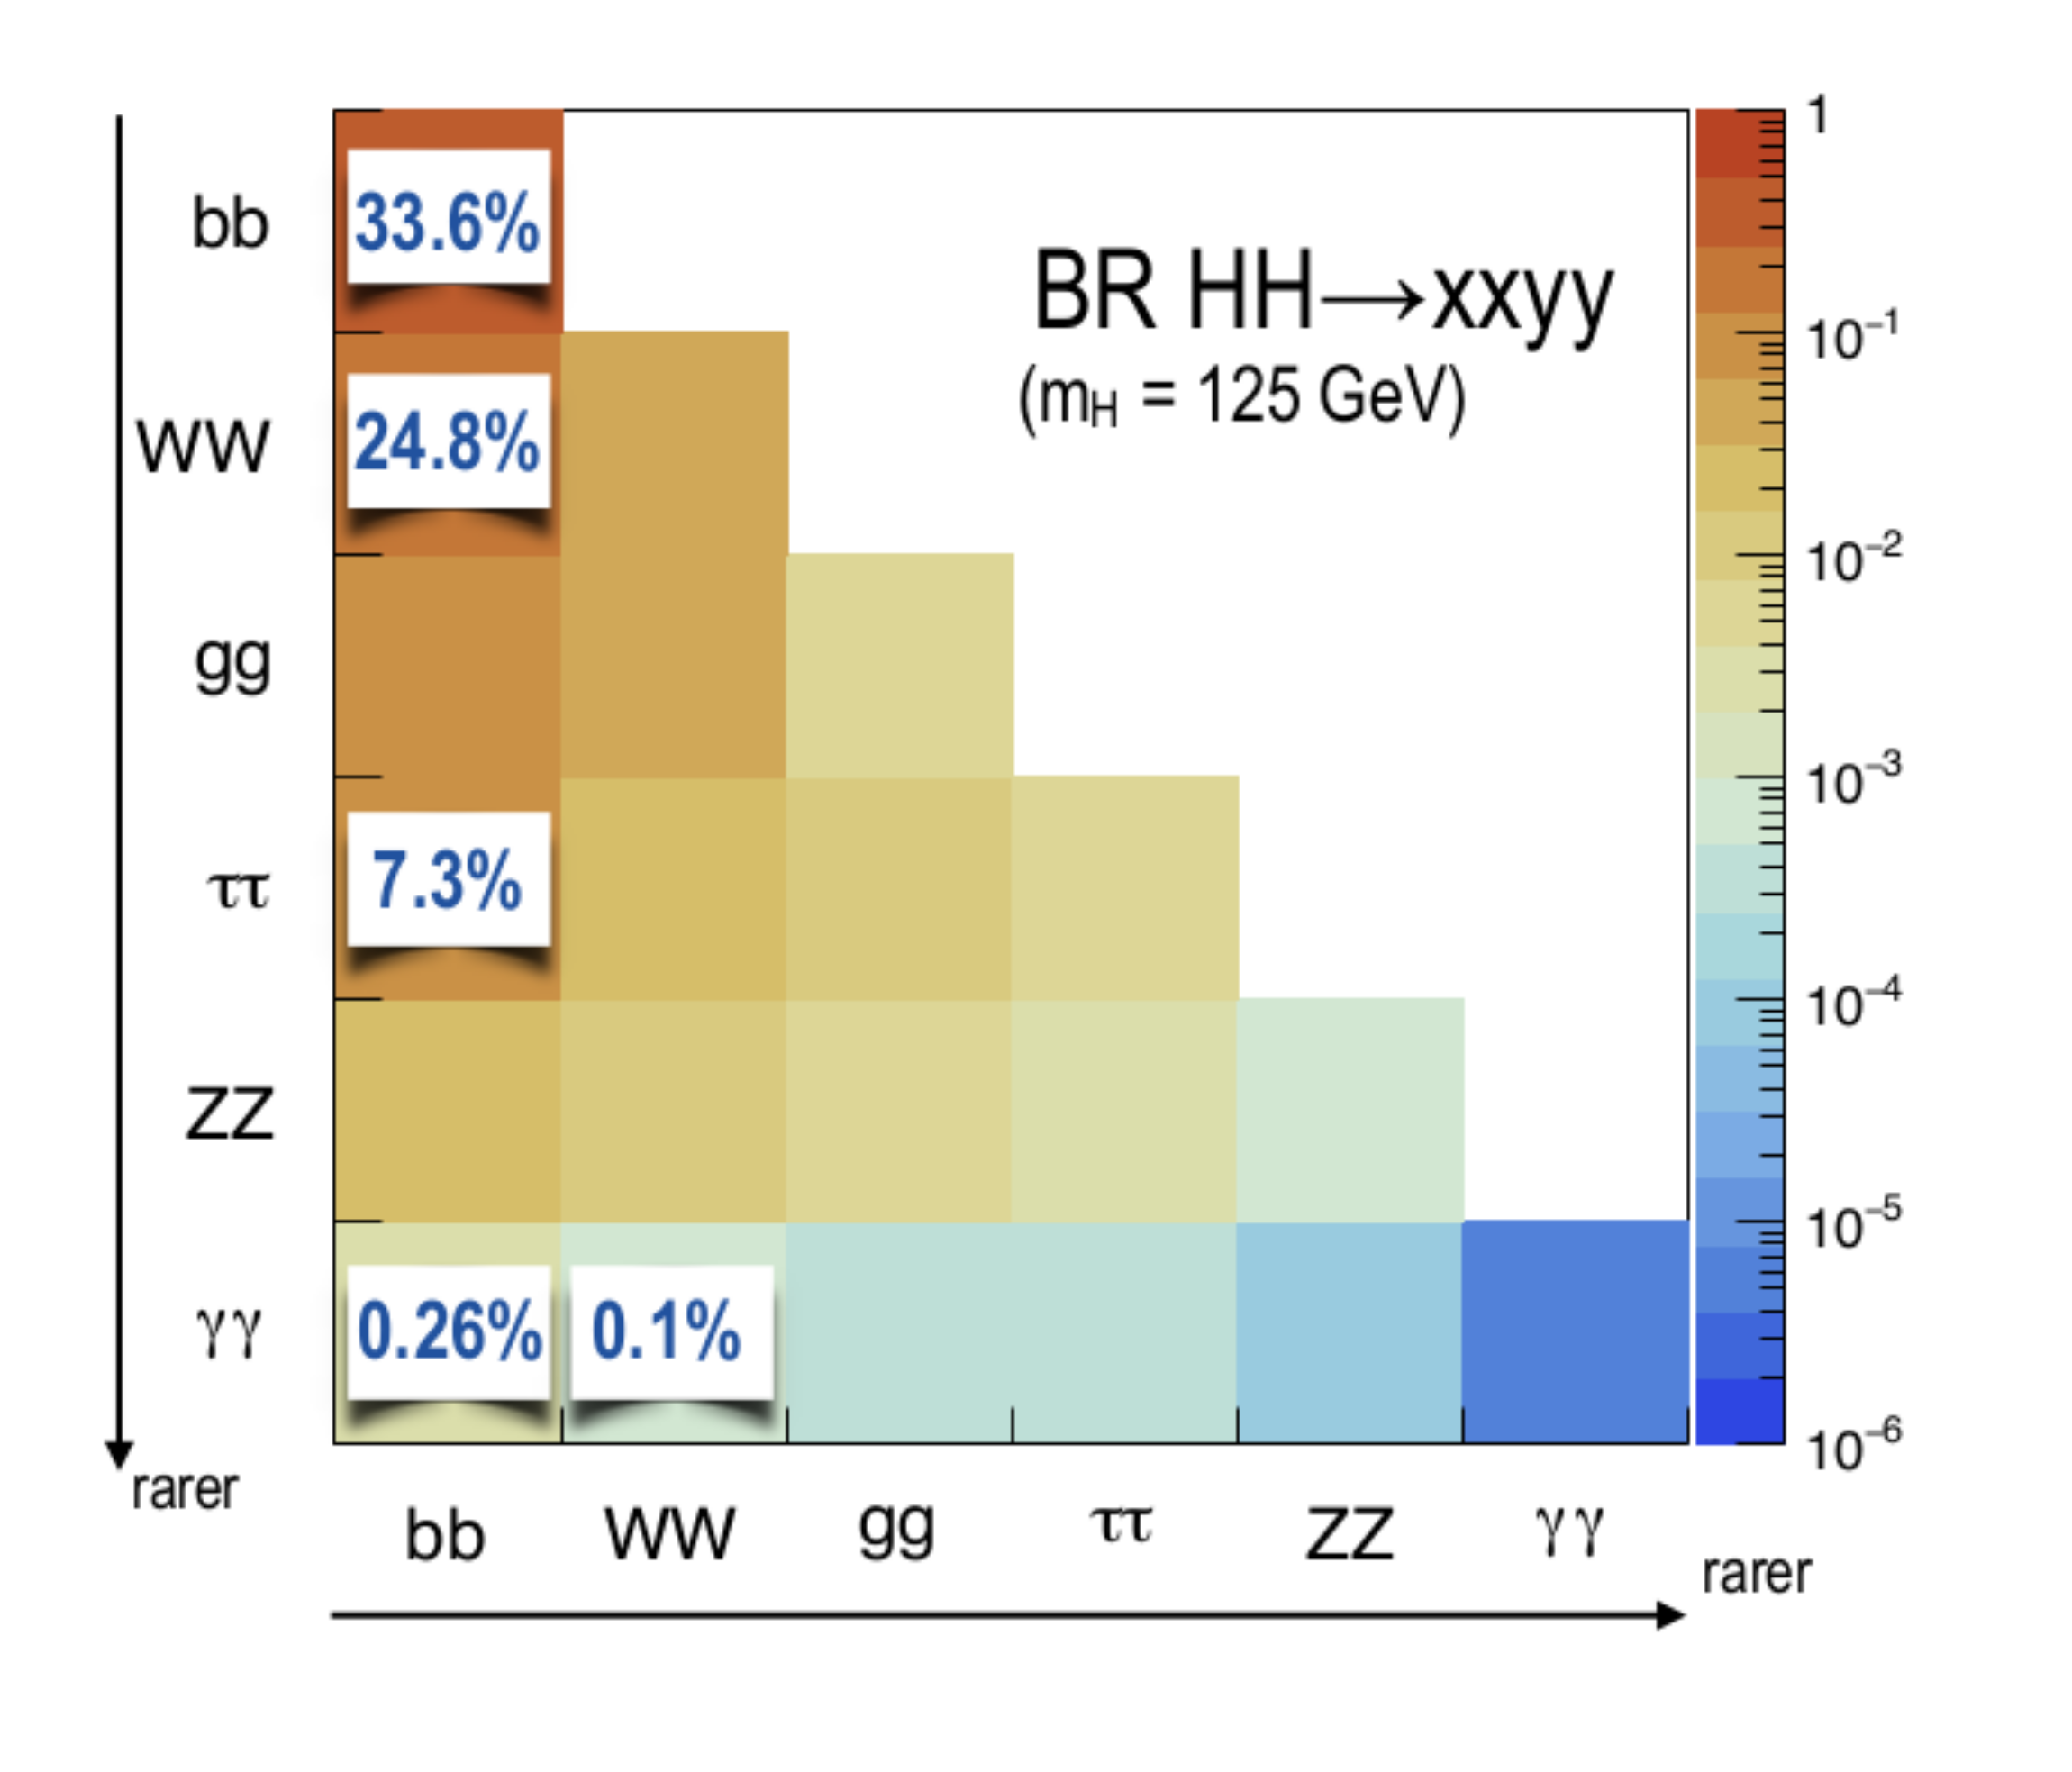
\includegraphics[width=\linewidth]{./Figures/hhBR.png}
	\end{minipage}%
	\begin{minipage}{.55\textwidth}
		\centering
		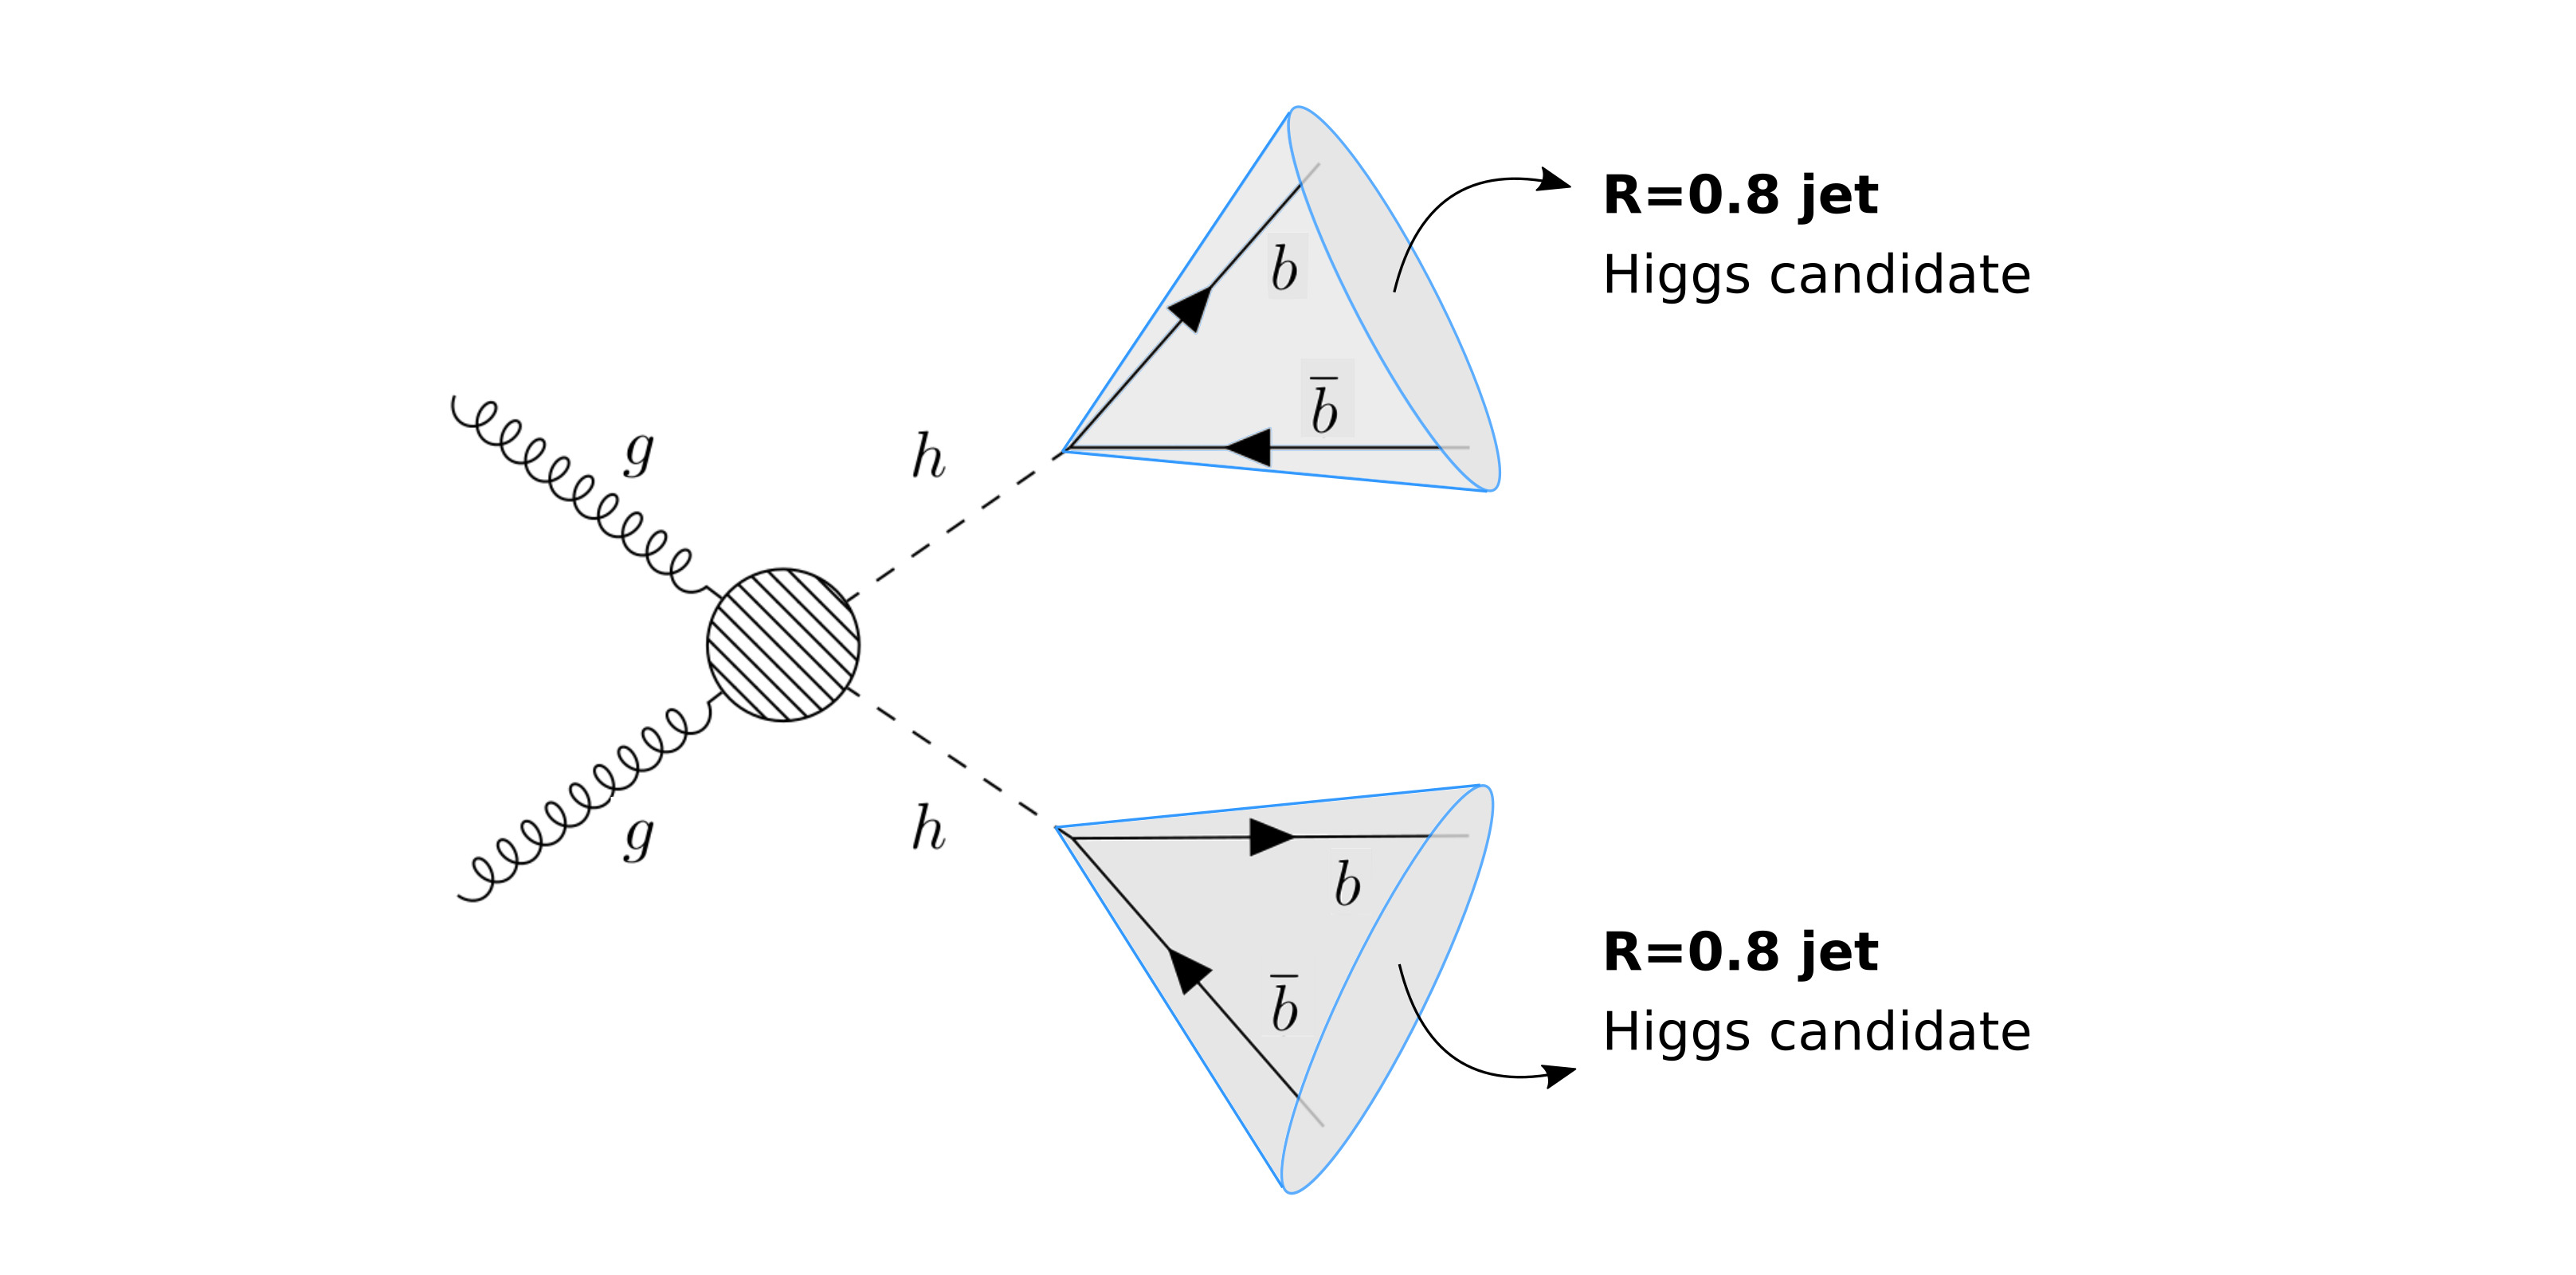
\includegraphics[trim={4cm 0 5cm 0},clip,width=\linewidth]{./Figures/boosted1.png}
	\end{minipage}
	\begin{minipage}[t]{0.45\textwidth}
		\caption*{(a)}
		%\label{fig1}
	\end{minipage}%%%
	\hfill
	\begin{minipage}[t]{0.55\textwidth}
		\caption*{(b)}
		%\label{fig2}
	\end{minipage}
	\caption{Higgs pairs branching ratios (left) and event topology targeted by this analysis (right).}
	\label{fig:boosted}
\end{figure}

%\begin{figure}
%	\centering
%	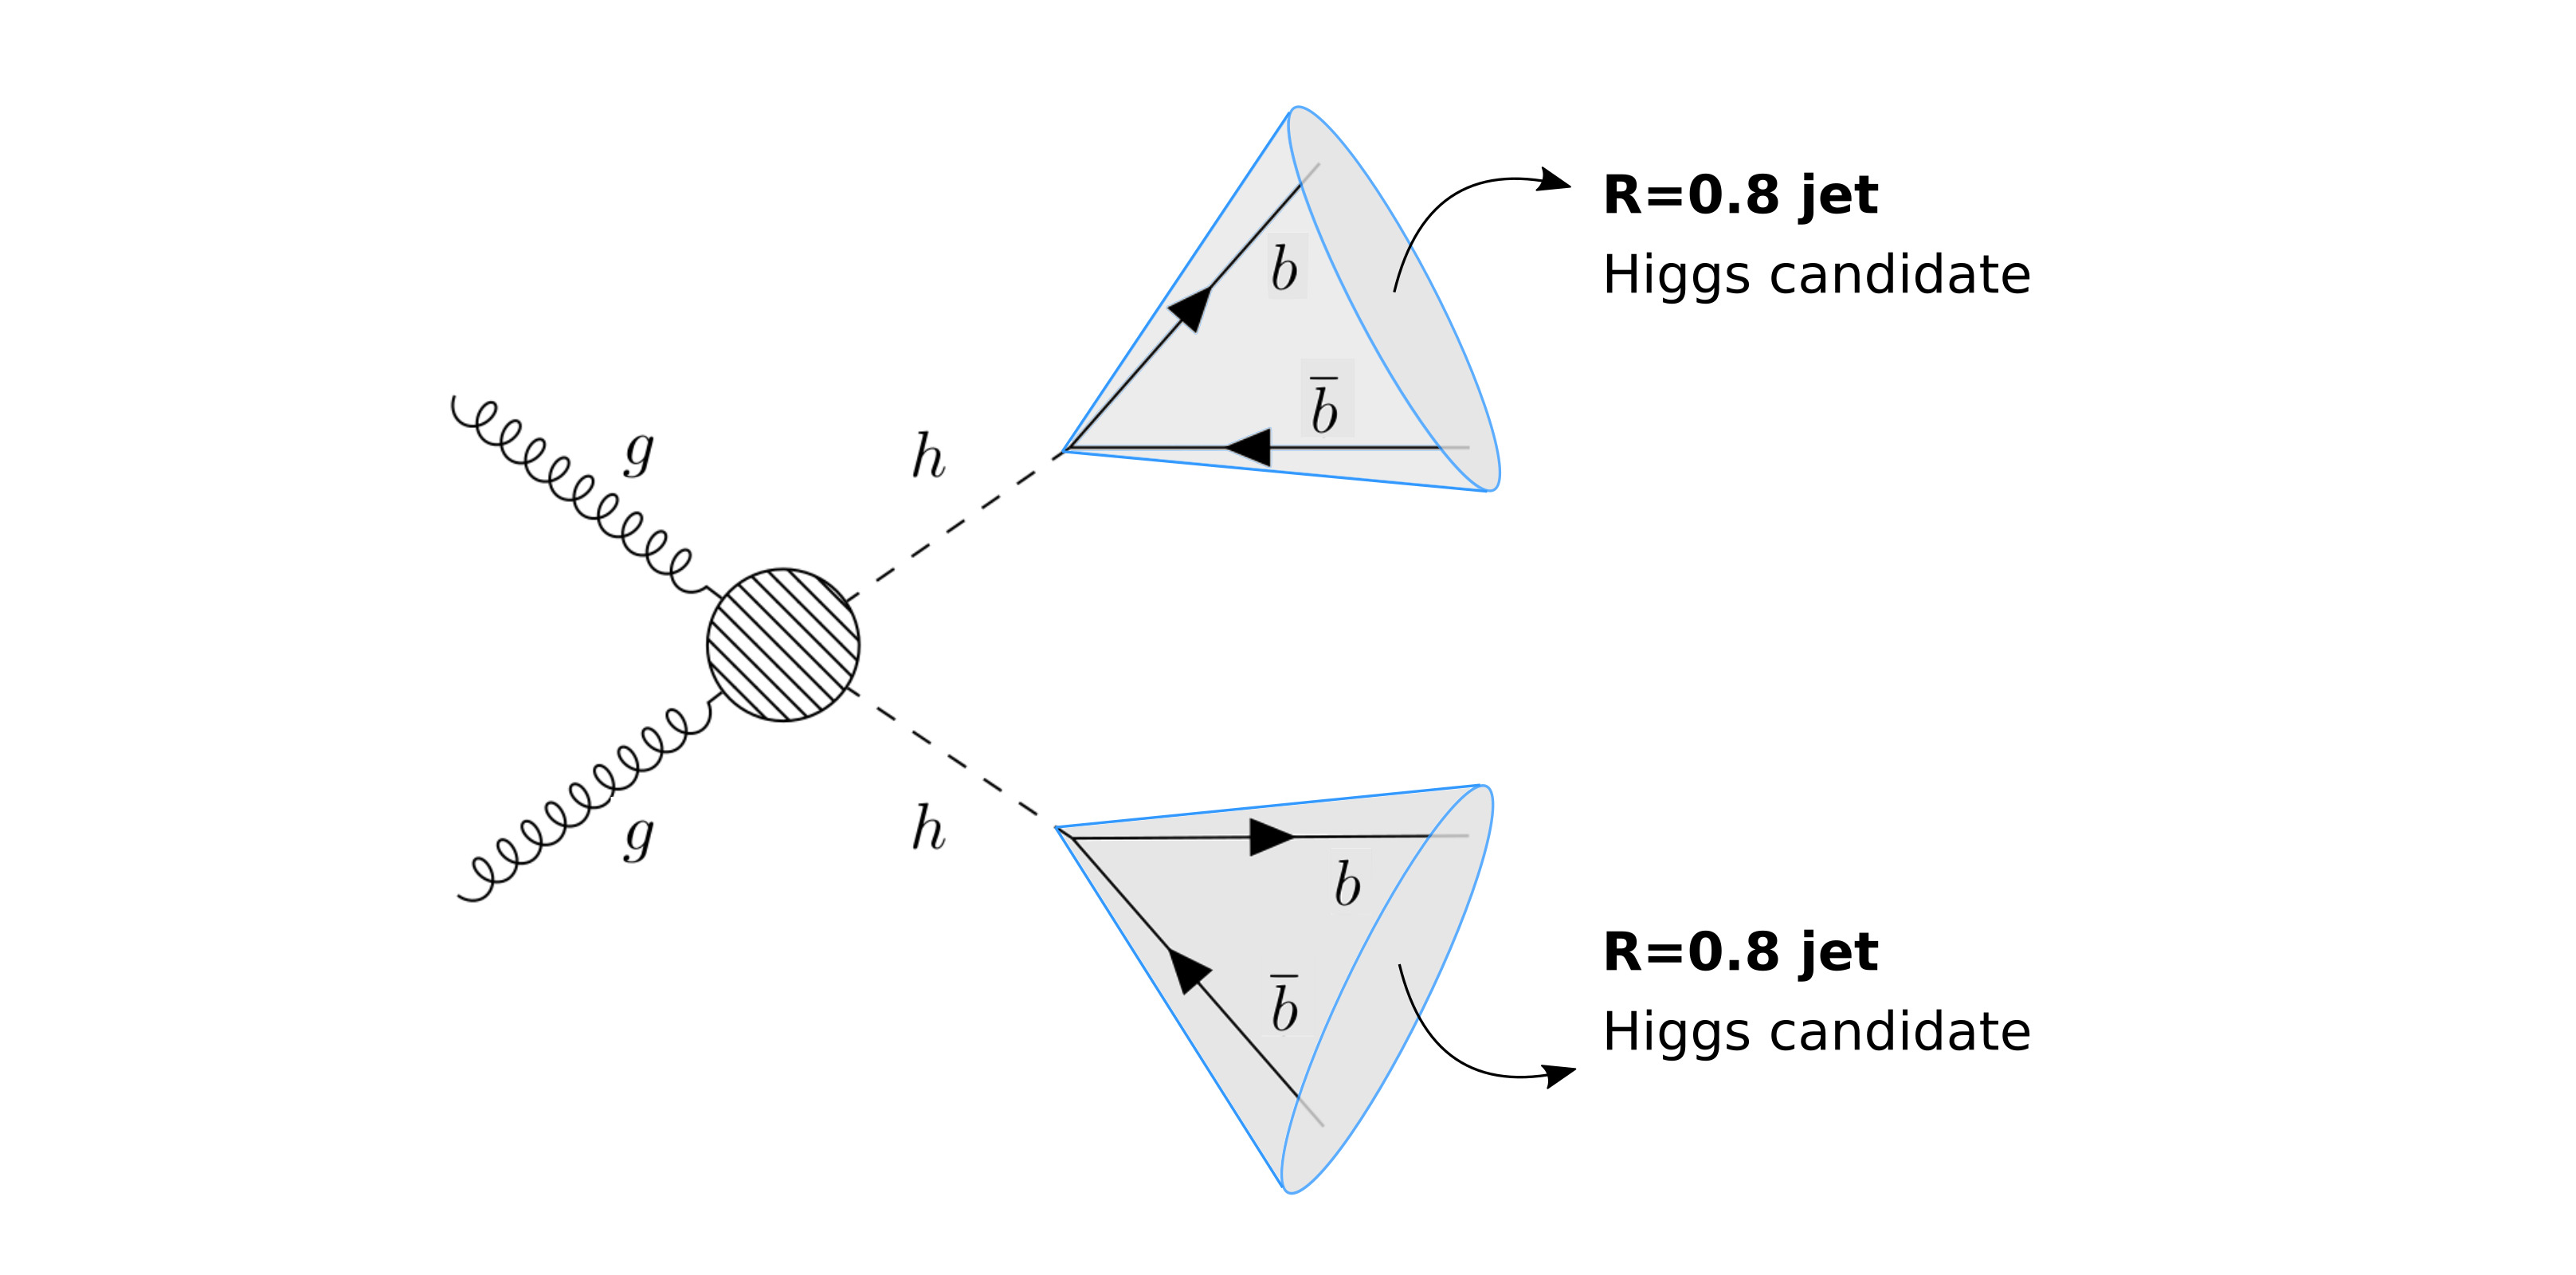
\includegraphics[width=\textwidth]{./Figures/boosted1.png}
%	%\hfill
%	%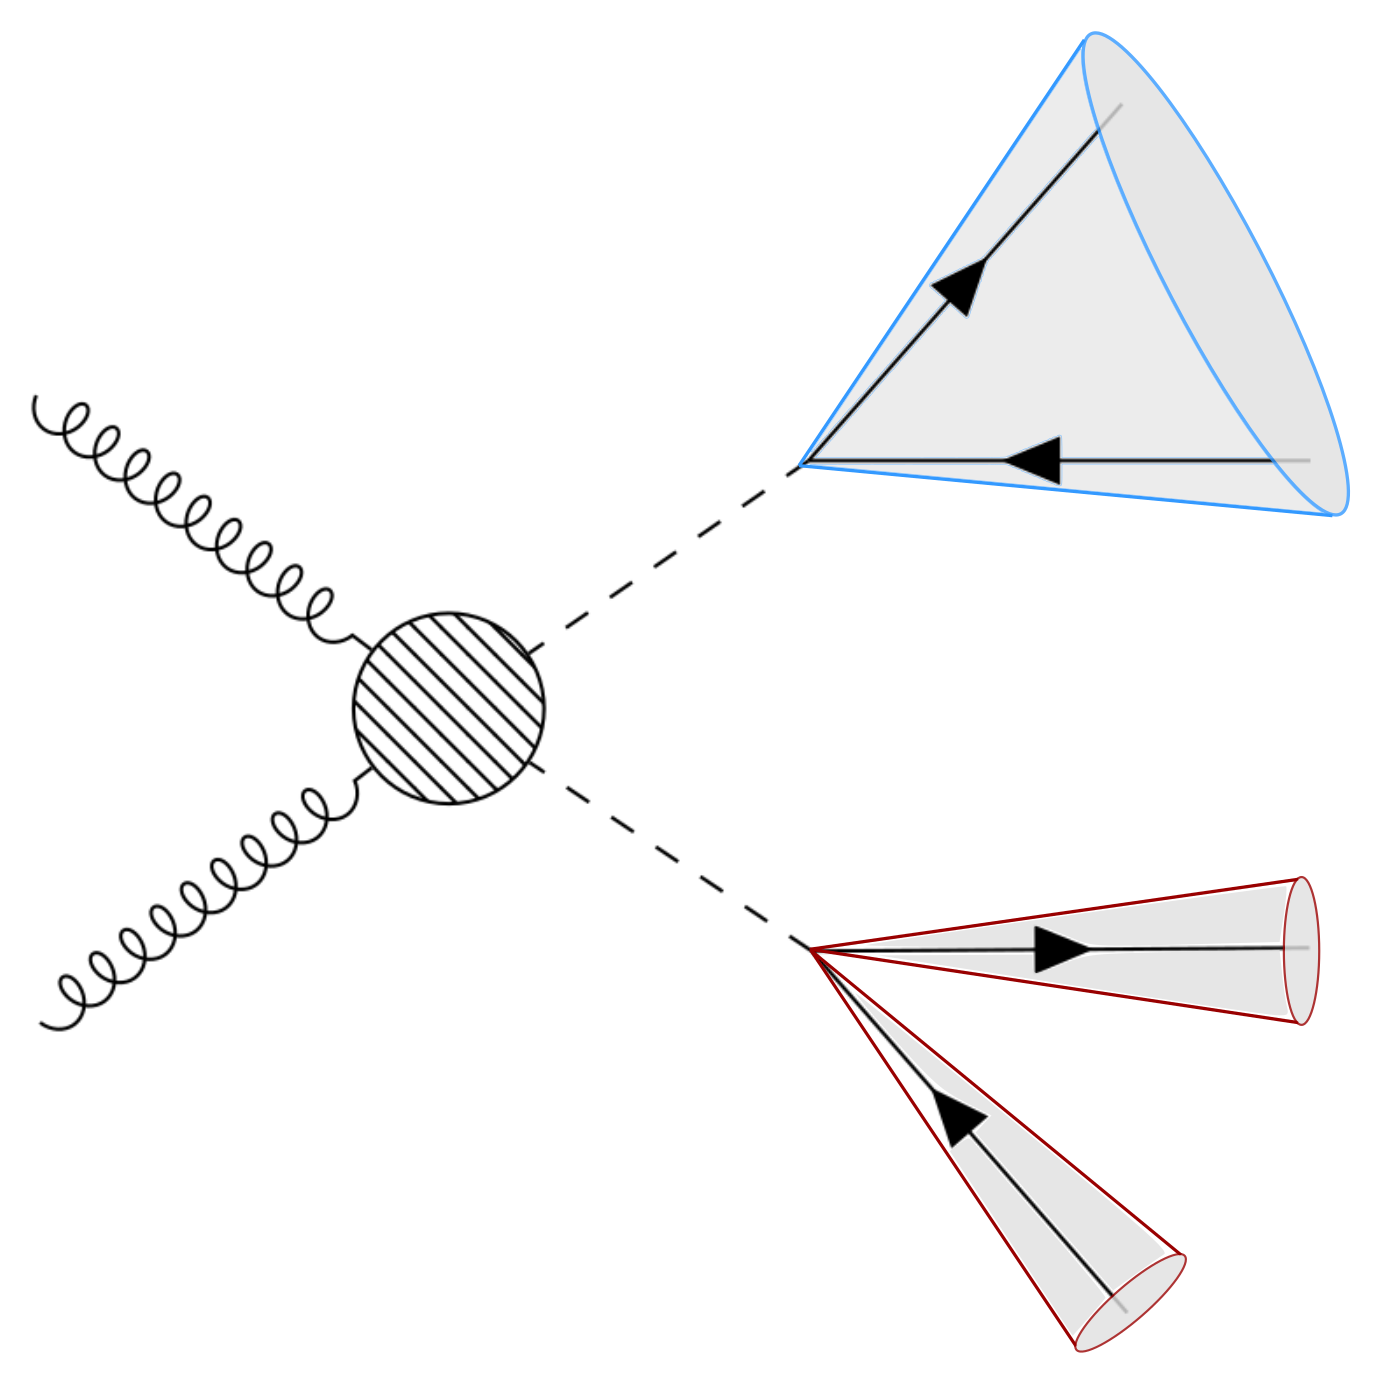
\includegraphics[width=.45\textwidth]{./Figures/inter.png}
%	\caption{Event topology targeted by the boosted analysis region. The blob represents the interaction between the gluons and the Higg bosons that is represented by the Feynman diagrams shown in figure \ref{fig:higgs_pair}.}
%	\label{fig:final_state}
%\end{figure}
%
%\begin{figure}
%	\centering
%	\includegraphics[width=0.6\textwidth]{./Figures/hhBR.png}
%	\label{fig:hhBR}
%	\caption{Higgs pair branching ratios.}
%\end{figure}

%The searches for Higgs pair production in the four b quarks final state benefit from the large BR of $h\rightarrow b\overline{b}$. 

For the SM Higgs, with a mass around $125$ GeV, the branching ratio of the $hh\rightarrow b\overline{b}b\overline{b}$ decay is approximately $33.6\%$, making it the most probable decay for Higgs pairs, as is illustrated in figure \ref{fig:boosted}(a).
%This leads to a cross section times BR of $\sim 0.7$ pb. 
However, in this channel, the main background is QCD multijet production that has a cross section several orders of magnitude larger than di-Higgs production in the SM, as table \ref{table:samples_summary} shows. Nonetheless, the jet $p_T$ distributions in this background have a very large yield close to zero and then fall very steeply while the signal has a much larger tail to high values of $p_T$. This indicates that searches targeting the boosted kinematic regime may be the key to measure $hh\rightarrow b\overline{b}b\overline{b}$ using inclusive production.

In this work we target the boosted regime. In this kinematic region, the final state of the signal is characterized by two jets with a large radius parameter. Each jet is expected to contain the two b quarks originated from the decay of a Higgs boson, as figure \ref{fig:boosted}(b) illustrates. Extra jets are also expected to be reconstructed as a consequence of QCD radiation. 

The analysis presented here is performed using the Monte-Carlo samples described in chapter \ref{chapter:tools}. All samples assume $m_h=125$ GeV. The event selection criteria are designed to optimize the significance, given by $S/\sqrt{B}$, where $S$ and $B$ represent the number of signal and background events, respectively. 

%In addition, the jets produced by QCD interaction are more likely to be initiated by a gluon or a light quark. Therefore, tight b-tagging criteria and algorithms based on substructure variables can also help reject this background. 

\subsection{Event pre-selection}

%TO INCLUDE: \\
%- discussion on trigger requirements: important in real analysis\\
%- show and discuss some distributions: invariant mass (h, hh), momentum, tau21, delta eta (hh), more substructure variables (may be all that we considered relevant)\\
%- compare with other articles/analysis ? \\

We start by applying very simple and loose cuts that target events consistent with the boosted topology. Jets are reconstructed with the anti-$k_T$ algorithm with an radius parameter $R=0.8$. They are reconstructed from particle flow objects or calorimeter towers. Both approaches were explored in this analysis.

We require at least two b-tagged $R=0.8$ jets which corresponds to at least four b-tagged subjets, at least two in each $R=0.8$ jet. The subjets are found through the soft drop mass technique that was described in section \ref{section:jet_groom}. The leading and sub leading jets must have $p_T\geq200$ GeV in order for the event to be accepted. From Eq. \ref{eq:deltaR}, a Higgs boson with, e.g., $p_T=200$ GeV leads to a pair of b quarks with $\Delta R\sim \frac{2m}{p_T}=1.25$. Therefore, considering jet with $R=0.8$ (diameter equal to $1.6$) and $p_T\geq 200$ GeV is a reasonable choice. For a more complete description about the jet radius see appendix \ref{chapter:jetrad}. Due to the b-tagging parameterization (described in detail in section \ref{sec:btagging}), there is a natural cutoff at $|\eta|=4$ so we do not place any additional cut in $\eta$. From now on, these cuts are referred to as pre-selection cuts.

After the pre-selection cuts we can plot all the relevant distributions that allow us to characterize the signal and background events. These are shown in the next two sections. In addition, these distributions provide a first insight into the discriminating power of the kinematic and substructure variables that are explored.  

\subsection{Signal characterization}

The cross section for di-Higgs inclusive production from $pp$ collisions at $100$ TeV is $1.22$ pb \cite{HxsNNLO}. This value is computed at NNLO accuracy. The dominant process is gluon-gluon fusion that has been extensively discussed in section \ref{section:Higgs_pair}. The signal process comprehends the di-Higgs inclusive production and the $hh\rightarrow b\overline{b}b\overline{b}$ subsequent decays. The total process cross section amounts to approximately $0.9$ pb. This number includes the branching ratio and a k-factor to account for known NNLL resuls. This is described in detail in section \ref{sec:Pythia_samples}. For an integrated luminosity of $30~\text{ab}^{-1}$ of proton-proton collisions at $\sqrt{s}=100$ TeV we expect $2.7\times 10^{7}$ events.

The Higgs candidates are reconstructed using large $R$ jets that can be directly measured using information from the calorimeters and tracking systems. Figure \ref{fig:deltaPhi_deltaR}(a) shows the $\Delta\phi$ between the two leading jets (Higgs candidates), $\Delta\phi(hh)$. For a large fraction of the signal events (red curve) $\Delta\phi(hh)\sim \pi$ which indicates that the jets are produced back-to-back in the transverse plane. There is also a small fraction of events for which the jets have $\Delta\phi(hh)\sim 1$. For these events there must be at least a third jet that balances the momentum of the jets pair. 

Each wide jet is expected to be consistent with having two subjets associated with the two b quarks from the $h\rightarrow b\overline{b}$ decay. In the Higgs rest frame, the two subjets are produced back-to-back conserving momentum. In the laboratory frame, the $\Delta R$ between the subjets depends on the momentum of the Higgs boson, with larger $\Delta R$ corresponding to Higgs bosons with a lower momentum. This correlation between the $\Delta R$ between the subjets of the leading Higgs candidate ($\Delta R(b\overline{b})$) and its momentum ($p_T(h_1)$) is shown in figure \ref{fig:deltaPhi_deltaR}(b). 

The $p_T$ distributions of the leading and sub leading jets (Higgs candidates) are shown in figures \ref{fig:h1h2_pt}(a) and \ref{fig:h1h2_pt}(b), respectively. The histograms are normalized to unit area in order to allow for shape comparison between them. For the leading jet, the signal $p_T$ spectrum peaks at approximately $350$ GeV and has a long tail for large values of $p_T$, in particular, longer than any of the backgrounds, at least up to $p_T>1000$ GeV. For the sub leading jet the spectrum is softer, as expected, but the tail of the distribution is still longer that for any of the backgrounds. These distributions show that the signal process produces jets with larger transverse momenta than the jets produce by the background processes which indicates that a boosted analysis might perform well.

The $\eta$ distribution of the leading jet is shown in figure \ref{fig:h1_eta_M}(a). This distribution is limited to $|\eta|<4$ because the b-tagging efficiency goes to zero for $|\eta|>4$ (see section \ref{sec:btagging} for more details). The number of events decreases as we go to larger values of $\eta$ which is due to the detector's acceptance. The $\eta$ distribution of the sub leading jet is very similar to this one so we abstain from showing it here.

The softdrop mass distribution of the leading jet is shown in figure \ref{fig:h1_eta_M}(b). For the signal (red curve) there is a clear peak at approximately $120$ GeV which corresponds to the SM Higgs boson mass peak. The peak is quite broad which means the mass resolution in this channel is not very good. On the one hand, this is because we are using large-$R$ jets to reconstruct the Higgs candidates. These objects have a worse mass resolution than other cleaner objects such as photons or electrons.  On the other hand, the cuts applied before plotting these distributions are very loose. As we place additional cuts the mass peak can be made slightly narrower. Another interesting feature of the signal mass spectrum is the existence of a peak close to zero. The explanation is the following: some jets do not contain both b quarks from the Higgs decay such that when applying the mass drop procedure only one b quark with a mass of approximately $5$ GeV remains inside the jet, creating the peak at lower masses. A more detailed discussion, as well as a plot that supports this interpretation, can be found in appendix \ref{chapter:SDmass}.

In addition to the basic kinematic distributions that we have just described, there are a multitude of other variables one can look at. Here we show the $\Delta\eta$ between the Higgs pairs, figure \ref{fig:hh_deltaEta_h1_tau21}(a), and the $\tau_{21}$ variable for the leading Higgs candidate, figure \ref{fig:hh_deltaEta_h1_tau21}(b). The first distribution shows that the Higgs pair tends to have a $\Delta\eta$ close to zero, which indicates that the pair is highly boosted in the longitudinal plane. The $\tau_{21}$ distribution shows that for the signal this variable takes values close to zero which means the jet is consistent with having two subjets.

\begin{figure}
	\centering
	\begin{minipage}{.5\textwidth}
		\centering
		\includegraphics[width=\linewidth]{./Figures/hist_hh_deltaPhi.pdf}
		%\caption{$\Delta\phi$ between the Higgs candidates.}
		%\label{fig:deltaR_bb_pt}
	\end{minipage}%
	\begin{minipage}{.5\textwidth}
		\centering
		\includegraphics[width=\linewidth]{./Figures/hist_deltaR_bb_pt.pdf}
		%\label{fig:hh_deltaPhi}
		%\caption{$\Delta R$ between the b quarks coming from the decay of the leading Higgs candidate, $h_1$. To obtain this plot the cut $|M-125|<40$ GeV was applied in addition to the pre-selection cuts.}
	\end{minipage}
	\begin{minipage}[t]{0.5\textwidth}
		\caption*{(a)}
		%\label{fig1}
	\end{minipage}%%%
	\hfill
	\begin{minipage}[t]{0.5\textwidth}
		\caption*{(b)}
		%\label{fig2}
	\end{minipage}
	\caption{$\Delta\phi$ between the Higgs candidates, $\Delta\phi(hh)$, (left) and $\Delta R$ between the b quarks coming from the decay of the leading Higgs candidate, $h_1$ (right). To obtain this plot the cut $|M-125|<40$ GeV was applied in addition to the pre-selection cuts..}
	\label{fig:deltaPhi_deltaR}
\end{figure}

%\begin{figure}
%	\centering
%	\includegraphics[width=0.7\linewidth]{./Figures/deltaR_bb_pt.pdf}
%	\label{fig:deltaR_bb_pt}
%	\caption{$\Delta R$ between the b quarks coming from the decay of the leading Higgs candidate, $h_1$. Plot obtained after the pre-selection cuts.}
%\end{figure}

%In the boosted regime, we expect at least two jets that are reconstructed using a large R parameter and that contain, each, the two b quarks that come from the decay of a Higgs boson. In the fully resolved regime, we expect at least four jets reconstructed with the standard R parameter of $0.4$, each corresponding to a b quark. Furthermore, an intermediate (or semi-resolved) category, in which one of the Higgs can be fully reconstructed using two small R jets and the other is reconstructed using a single large-R jet can also be explored. In all categories, we expect the presence of extra jets due to QCD activity. 

\subsection{Backgrounds}

The relevant backgrounds for this analysis are QCD multijet production, $t\overline{t}$ and $b\overline{b}b\overline{b}$. Although the $b\overline{b}b\overline{b}$ background is a particular case of a QCD multijet production process we consider it separately because it constitutes the irreducible background and therefore will have a higher efficiency in the analysis. The cross sections for these processes are several orders of magnitude larger than the cross section for the signal, as table \ref{table:samples_summary} shows. In addition, in the case of the $t\overline{t}$ background, the event topology is expected to be similar to the signal because it also consists in the production of a pair of particles with the same mass.

The assumption that QCD multijet production and $t\overline{t}$ are the two main backgrounds is corroborated by the ATLAS di-Higgs search performed in the same channel, where these backgrounds are found to be the dominant ones. All other sources of backgrounds, including processes involving Higgs bosons, are found to be negligible \cite{hh2bbbbATLAS}. In appendix \ref{chapter:bkgHiggs} we discuss and evaluate the importance of some backgrounds that include Higgs bosons in our analysis.

Figure \ref{fig:QCD} shows examples of LO Feynman diagrams that contribute to $4b+~j$ (left), three (middle) and four (right) light jets production. The $b\overline{b}b\overline{b}$ background is generated with an extra light jet at generator level, as discussed in chapter \ref{chapter:tools}. This jet boosts the four b quarks and has a minimum $p_T$ of $200$ GeV. This increases the probability of two b quarks being reconstructed as single large-$R$ jet therefore emulating the signal's final state signature, i.e, high $p_T$ jets compatible with a two-prong substructure. The QCD $4b+j$ sample with $(200<p_T<500)$ GeV has a cross section of approximately $756$ pb. In addition, as explained in section \ref{sec:Pythia_samples}, we multiply this cross section by a k-factor of $2$, which yields a total cross section of approximately $1.5\times 10^{3}$ pb. The cross section is a lot smaller for the other $4b+j$ QCD sample as well as for the samples that include both QCD and eletroweak contributions, as expected.

The QCD multijet background consists of two, three and four jet events (represented as $jj+0/1/2 ~j$), at generator level. The jets can originated from light and b quarks and from gluons. A jet matching procedure is implemented in Pythia in order to avoid double counting. Due to mis-tagging probabilities, light and c jets can be identified as b jets. Although these probabilities are relatively small when compared to the b-tagging efficiency (see section \ref{sec:btagging}) the cross section of multijet processes is very large such that this background becomes dominant. The $jj+0/1/2 ~j$ sample with $(500<H_T<1000)$ GeV has a cross section of the order of $10^7$ GeV. As anticipated, the $p_T$ spectrum of the multijet background is a lot softer than for the signal and remaining backgrounds, as it is shown in figures \ref{fig:h1h2_pt}(a) and \ref{fig:h1h2_pt}(b). In addition, for this background the $\tau_{21}$ variable takes values close to one, as it is shown in figure \ref{fig:hh_deltaEta_h1_tau21}(b). This indicates that the jets are not consistent with two subjets. 

Figure \ref{fig:tt} shows examples of LO Feynman diagrams that contribute to $t\overline{t}$ production through $q\overline{q}$ (left) and $gg$ (middle and right) fusion. The $t\overline{t}$ background is simulated with additional zero, one or two jets (represented as $t\overline{t}+0/1/2 ~j$), at generator level. The extra jets can originated from light and b quarks and from gluons. A jet matching procedure is implemented in Pythia in order to avoid double counting. The top quark has a very short life time, predicted to be $5\times 10^{-25}$ s, such that it decays before it can hadronize. This sample is inclusive in the top quark decay modes. However, the most favoured decay of the top quark is $t\rightarrow Wb$ with a branching ratio close to $96\%$ \cite{PDG2016}. Therefore, $t\overline{t}$ events will, most of the times, result in the $W^+W^-b\overline{b}$ final state. We do not specify any decay mode for the $W$ such that the sample is also inclusive in the $W$ decay modes. The $W$ decays to hadrons $(W^+\rightarrow q\overline{q})$ and leptons $(W^+\rightarrow l^+\nu)$ with BR$(W^+\rightarrow q\overline{q})\sim 68\%$ and BR$(W^+\rightarrow l^+\nu)\sim 10\%$. If one (or both) $W$ bosons decays to hadrons then there will be additional jets in the final state. These can be b jets or can be misidentified as such. If both $W$ bosons decay to leptons there will still be at least two b jets in the final state, coming from the $t\overline{t}$ decay. The cross section of the $t\overline{t}+0/1/2 ~j$ is approximately $4.3\times 10^4$ pb. As explained in \ref{sec:Pythia_samples}, k-factor of $1.74$ is applied which yields a total cross section of approximately $7.5\times 10^{4}$ pb.

It is interesting to note that in the softdrop mass plot for the leading Higgs candidate (figure \ref{fig:h1_eta_M}(b)) the $t\overline{t}$ background (green line) shows a small peak around $170$ GeV. In this region, all the decay products of the top quark are contained inside the $R=0.8$ jet such that the jet mass corresponds to the mass of the original top quark.

%In addition, we also take into account the irreducible background, $b\overline{b}b\overline{b}$ because it is expected to be the background with the highest efficiency.

\begin{figure}
	\centering
	\feynmandiagram[small,layered layout,horizontal=i1 to a] {% Draw the top and bottom lines
		i1 [particle=\(\overline{q}\)]-- [anti fermion] a-- [boson, edge label'=\(g/h/Z/\gamma\)]  b,
		i2 [particle=\(q\)]-- [fermion] c-- [gluon, edge label=\(g\)] d,
		% Draw the two internal fermion lines
		{ [  same layer] a -- [anti fermion] c},
		%f1  -- [fermion] b -- [fermion] f2 ,
		%f3  -- [fermion] f2 -- [gluon] g1 ,
		%f4  -- [fermion] g1 -- [fermion] f5 ,
		%	a -- [opacity=0.2] c,
		%g1 -- [anti fermion] b,
		b -- [anti fermion] f2 [particle=\(\overline{b}\)],
		b -- [fermion] f3 ,
		f3 -- [fermion] f4 [particle=\(b\)],
		f3 -- [boson, edge label'=\(g/h/Z/\gamma\)] g1,
		g1 -- [anti fermion] f5 [particle=\(\overline{b}\)],
		g1 -- [fermion] f6 [particle=\(b\)],
	};\qquad
	\feynmandiagram[small,layered layout,horizontal=a to b] {% Draw the top and bottom lines
		i1 [particle=\(\overline{q}\)]-- [anti fermion] a-- [anti fermion]  b,
		i2 [particle=\(q\)]-- [fermion] c-- [fermion] d [particle=\(q\)],
		% Draw the two internal fermion lines
		{ [  same layer] a -- [gluon] c},
		%f1  -- [fermion] b -- [fermion] f2 ,
		%f3  -- [fermion] f2 -- [gluon] g1 ,
		%f4  -- [fermion] g1 -- [fermion] f5 ,
		%	a -- [opacity=0.2] c,
		%g1 -- [anti fermion] b,
		b -- [anti fermion] f2 [particle=\(\overline{q}\)],
		b -- [gluon] f3 [particle=\(g\)],
	};\qquad
	\feynmandiagram
	[horizontal=a to b] {i1 [particle=\(q\)] -- [fermion] a -- [fermion] i2 [particle=\(\overline{q}\)],
		a -- [gluon] b,
		g1 -- [gluon] b -- [gluon] g2,
		f1 [particle=\(\overline{q}\)] -- [fermion] g1 -- [fermion] f2 [particle=\(q\)],
		f3 [particle=\(\overline{q}\)] -- [fermion] g2 -- [fermion] f4 [particle=\(q\)],
		g1 -- [opacity=0] g2,
		f2 -- [opacity=0] f4,
	};
	%		\feynmandiagram[small,layered layout,horizontal=i1 to a] {% Draw the top and bottom lines
	%			i1 [particle=\(\overline{q}\)]-- [anti fermion] a-- [boson, edge label'=\(h/Z/\gamma\)]  b,
	%			i2 [particle=\(q\)]-- [fermion] c-- [gluon, edge label=\(g\)] d,
	%			% Draw the two internal fermion lines
	%			{ [  same layer] a -- [anti fermion] c},
	%			%f1  -- [fermion] b -- [fermion] f2 ,
	%			%f3  -- [fermion] f2 -- [gluon] g1 ,
	%			%f4  -- [fermion] g1 -- [fermion] f5 ,
	%			%	a -- [opacity=0.2] c,
	%			%g1 -- [anti fermion] b,
	%			b -- [anti fermion] f2 [particle=\(\overline{b}\)],
	%			b -- [fermion] f3 ,
	%			f3 -- [fermion] f4 [particle=\(b\)],
	%			f3 -- [boson, edge label'=\(h/Z/\gamma\)] g1,
	%			g1 -- [anti fermion] f5 [particle=\(\overline{b}\)],
	%			g1 -- [fermion] f6 [particle=\(b\)],
	%		};
	\caption{Example of diagrams that contribute to the QCD multijet background: five final state jets, four of which are b-jets (left), three final state jets (middle) and four final state jets (right). Here, $q$ stands for a light quark/jet.}
	\label{fig:QCD}
\end{figure}

\begin{figure}
\centering
\feynmandiagram
[horizontal=a to b] {i1 [particle=\(q\)] -- [fermion] a -- [fermion] i2 [particle=\(\overline{q}\)],a -- [gluon,edge label=\(g\)] b, f1 [particle=\(t\)] -- [fermion] b -- [fermion] f2 [particle=\(\overline{t}\)],
};\qquad
\feynmandiagram
[horizontal=a to b] {i1 [particle=\(g\)] -- [gluon] a -- [gluon] i2 [particle=\(g\)],a -- [gluon,edge label=\(g\)] b, f1 [particle=\(t\)] -- [fermion] b -- [fermion] f2 [particle=\(\overline{t}\)],
}; \qquad
\feynmandiagram[layered layout,horizontal=a to b] {% Draw the top and bottom lines
	i1 [particle=\(g\)]-- [gluon] a-- [anti fermion]  b [particle=\(\overline{t}\)] -- ,i2 [particle=\(g\)]-- [gluon] c-- [fermion] d [particle=\(t\)] -- ,
	% Draw the two internal fermion lines
	{ [  same layer] a -- [fermion] c},
};
\caption{Dominant diagrams of $pp\rightarrow t\overline{t}$ at LO.}
\label{fig:tt}
\end{figure}


%\begin{figure}[h]
%	\centering
%	\feynmandiagram [horizontal=b to c] {
%		a -- [gluon] b [blob],c -- [scalar] b-- [gluon] d,
%		c -- [scalar] e,
%		c -- [scalar] f,
%		e -- [fermion] g,
%		e -- [anti fermion] h,
%		f -- [fermion] i,
%		f -- [anti fermion] j,
%	};
%	\caption{Final state}
%\end{figure}

%\begin{figure}[h]
%	\centering
%	\feynmandiagram [horizontal=d to h] {
%		a [particle=\(g\)] -- [gluon] b [blob],
%		c [particle=\(g\)] -- [gluon] b -- [gluon],
%		d -- [scalar, edge label'=\(h\)] b -- [scalar],
%		e -- [scalar, edge label'=\(h\)] b -- [scalar],
%		d -- [fermion, edge label=\(b\)] g ,
%		d -- [anti fermion, edge label=\(\overline{b}\)] h ,
%		e -- [fermion, edge label'=\(b\)] i,
%		e -- [anti fermion, edge label'=\(\overline{b}\)] j ,
%		d -- [opacity=0] e,
%		%h -- [opacity=0] i,
%		g -- [opacity=0] h,
%		i -- [opacity=0] j,
%		h -- [opacity=0] i,
%	};
%	\caption{Final state}
%\end{figure}




%\begin{table}
%	\centering
%	\begin{tabular}{lp{30mm}p{10mm}p{30mm}p{30mm}}
%		\toprule 
%		Pythia & hh (h$\rightarrow b\overline{b}$) & 4b+j & jj+0/1/2 j & tt+0/1/2 j \\
%		\midrule
%		Relevant settings & 25:onMode=off \newline 25:onIfAny= 5 -5&  & \textbf{Jet matching:} \newline merge=on \newline scheme=1 \newline setMad=off \newline coneRadius=1.0 \newline etaJetMax=10 \newline nJetMax=4 \newline qCut=30 & \textbf{Jet matching:} \newline merge=on \newline scheme=1 \newline setMad=off \newline coneRadius=1.0 \newline etaJetMax=10 \newline nJetMax=2 \newline qCut=60\\
%		\rowcolor{black!7} Description & Turn on the $h\rightarrow b\overline{b}$ decay for the undecayed Higgs. &  &  \multicolumn{2}{l}{Set parameters for jet matching procedure. } \\
%		\bottomrule
%	\end{tabular}
%	\caption{oi}
%	\label{table:DelphesHCAL}
%\end{table}

\begin{figure}
	\centering
	\begin{minipage}{.5\textwidth}
		\centering
		\includegraphics[trim={.65cm 0 0 0},clip,width=\linewidth]{./Figures/hist_h1_pt.pdf}
		%\caption{oi}
		%\label{fig:h1_pt}
	\end{minipage}%
	\begin{minipage}{.5\textwidth}
		\centering
		\includegraphics[trim={0 0 .65cm 0},clip,width=\linewidth]{./Figures/hist_h2_pt.pdf}
		%\caption{oi}
		%\label{fig:h2_pt}
	\end{minipage}
	\begin{minipage}[t]{0.5\textwidth}
		\caption*{(a)}
		%\label{fig1}
	\end{minipage}%%%
	\hfill
	\begin{minipage}[t]{0.5\textwidth}
		\caption*{(b)}
		%\label{fig2}
	\end{minipage}
	\caption{$p_T$ distributions for the leading (left) and sub leading (right) Higgs candidates. The signal is the SM $hh\rightarrow b\overline{b}$ process. The histograms are normalized to unit area.}
	\label{fig:h1h2_pt}
\end{figure}

\begin{figure}
	\centering
	\begin{minipage}{.5\textwidth}
		\centering
		\includegraphics[trim={.65cm 0 0 0},clip,width=\linewidth]{./Figures/hist_h1_eta.pdf}
		%\caption{oi}
		%\label{fig:h1_pt}
	\end{minipage}%
	\begin{minipage}{.5\textwidth}
		\centering
		\includegraphics[trim={0 0 .65cm 0},clip,width=\linewidth]{./Figures/hist_h1_softdrop_M.pdf}
		%\caption{oi}
		%\label{fig:h2_pt}
	\end{minipage}
	\begin{minipage}[t]{0.5\textwidth}
		\caption*{(a)}
		%\label{fig1}
	\end{minipage}%%%
	\hfill
	\begin{minipage}[t]{0.5\textwidth}
		\caption*{(b)}
		%\label{fig2}
	\end{minipage}
	\caption{$\eta$ distribution for the leading Higgs candidate (left) and softdrop mass distribution for the leading Higgs candidate (right). The signal is the SM $hh\rightarrow b\overline{b}$ process. The histograms are normalized to unit area.}
	\label{fig:h1_eta_M}
\end{figure}	

\begin{figure}
	\centering
	\begin{minipage}{.5\textwidth}
		\centering
		\includegraphics[trim={.65cm 0 0 0},clip,width=\linewidth]{./Figures/hist_hh_deltaEta.pdf}
		%\caption{oi}
		%\label{fig:h1_pt}
	\end{minipage}%
	\begin{minipage}{.5\textwidth}
		\centering
		\includegraphics[trim={0 0 .65cm 0},clip,width=\linewidth]{./Figures/hist_h1_tau21.pdf}
			%\caption{oi}
			%\label{fig:h2_pt}
	\end{minipage}
	\begin{minipage}[t]{0.5\textwidth}
		\caption*{(a)}
			%\label{fig1}
	\end{minipage}%%%
	\hfill
	\begin{minipage}[t]{0.5\textwidth}
		\caption*{(b)}
			%\label{fig2}
	\end{minipage}
	\caption{Distributions of the $\Delta\eta$ between the Higgs candidates (left) and of the $\tau_{21}$ variable for the leading Higgs candidate (right).  The histograms are normalized to unit area.}
	\label{fig:hh_deltaEta_h1_tau21}
\end{figure}
	

\section{Analysis strategy}
\label{section:regions}


%In this analysis we explore three regions: boosted, intermediate and resolved. The details about each region, namely the event topology and selection cuts, are discuss in the following sections (\ref{section:boosted}, \ref{section:intermediate} and \ref{section:resolved}). The regions are orthogonal, i.e, independent. For each event we check if it falls in the boosted category. If it does not we check if it falls in the intermediate category and if it does not we check if it falls in the resolved category. This way, an event falling in the boosted category cannot fall in the intermediate or resolved categories and the same applies for all categories. 
%
%The advantage of performing an analysis in orthogonal regions is that we can then combine the results obtained in each one. For example, we can quadratically add the significances in order to obtained an overall significance. This would not be possible if there were any overlap between the regions. In addition, we have access to increased statistics because we are exploring three different signal topologies. Nonetheless, the selection criteria for each category, as well as the variables to explore, are different and need to be optimized independently.

%- Event topology: two boosted jets each corresponding to a Higgs \\
%- Physics objects: partile flow anti-kT R=0.8 jets (discussion about jet radius in appendix) \\
%- Selection criteria\\
%- Substructure variables \\
%- Optimization (efficiency plots, correlations, MVA...)\\


%\begin{figure}
%	\centering
%	\includegraphics[width=\textwidth]{./Figures/boosted1.png}
%	%\hfill
%	%\includegraphics[width=.45\textwidth]{./Figures/inter.png}
%	\caption{Event topology targeted by the boosted analysis region. The blob represents the interaction between the gluons and the Higg bosons that is represented by the Feynman diagrams shown in figure \ref{fig:higgs_pair}.}
%	\label{fig:final_state}
%\end{figure} 

%In this analysis is focused on the bosoted regime. It targets events in which the Higgs bosons have a high Lorentz boost which leads to the collimation of the pairs of b quarks resulting from their decay. As a result, the b quarks cannot be reconstructed in four separated jets. Therefore, two pairs of b quarks are reconstructed using two jets with a larger R parameter. Each jet is expected to contain the b quarks coming from one of the Higgs bosons and works as a proxy for the properties of that Higgs boson.

As already discussed, this analysis targets events in which at least two large-$R$ jets are reconstructed. The jet with the highest momentum is assumed to correspond to the leading Higgs candidate and the jet with the second highest momentum to the sub leading one. Both the leading and sub leading jets must be b-tagged in order for the event to be accepted.

The events are reconstructed using particle flow (or eflow) or pure calorimeter jets (we explored both approaches) with $R=0.8$, clustered with the anti-$k_T$ algorithm. We perform the b-tagging of jets using truth level information as it is described in the following section. Jets with a large-$R$ parameter cannot be b-tagged using Delphes default algorithm because the tagging of large R jets is an ambiguous task that can be performed in several different ways. Therefore, we implemented our own b-tagging algorithm that is described in section \ref{sec:btagging}. 

In this section, we present the baseline analysis based on cuts on the kinematic and substructure variables. An optimized version of the analysis is also presented and compared to the baseline. The optimization is based on plots of the significance ($S/\sqrt{B}$) as a function of the cut on a given variable. We also briefly describe how statistical uncertainties are taken into account. 

\subsection{Implementation of b-tagging}
\label{sec:btagging}

\begin{figure}
	\centering
	\includegraphics[width=0.5\textwidth]{./Figures/deltaR_bsubjet}
	\caption{Minimun $\Delta R$ between b quarks and subjets of the $R=0.8$ jets.} 
	\label{fig:deltaR_bsubjet}
\end{figure}

For each jet, the two hardest subjets are found using the mass drop procedure. It might happen that there are not two subjets because the algorithm's criteria are not met. In that case, the jet is rejected. We compute the $\Delta R$ distance between all b and c quarks in the event with Pythia 8 status equal to $23$ and with $p_T>10$ GeV and each subjet ($\Delta R(\text{subjet,parton})$). According to the Pythia manual, particles with status $23$ result directly from the hardest subprocess. We consider that a subjet is matched to a given quark if $\Delta R(\text{subjet,parton})<0.3$, as indicated by the plot in figure \ref{fig:deltaR_bsubjet}. If the subjet is matched to at least a b quark, we b-tag the subjet with a given probability. If the subjet is not matched to any b quark but it is matched to at least one c quark we apply a c mistag rate. If the subjet is not matched to any b or c quark we apply a light mis tag rate. The b-tag probability and mistag rates were obtained from the Delphes FCC-hh card. They depend on the momentum of the jet and on its $\eta$ coordinate. They are summarized in table \ref{table:btag}. The b-tagging probabilities are given in black and the c and light mis tagging probabilities are given in blue and red, respectively. Note that a jet cannot be b-tagged if $|\eta|>4$ or if its momentum is smaller than $10$ GeV or larger than $15000$ GeV.

In terms of the technical implementation, the b-tagging algorithm works as follows: for each subjet we look for a truth-level b quark within $\Delta R=0.3$ of the subjet and calculate the b-tagging and mis-tagging efficiencies using the expressions in table \ref{table:btag}, where $p_T$ and $\eta$ refer to the subjet. If a b quark is found we generate a random number between $0$ and $1$. If it smaller that the b-tagging efficiency we consider the subjet to be b-tagged. If the subjet is not b-tagged we look for truth-level c quarks within $\Delta R=0.3$ of the subjet. If one is found we generate a new random number between $0$ and $1$ and if the number is smaller than the c mis-tag probability we consider the subjet to be b-tagged. If the subjet is not b-tagged we generate a random number between $0$ and $1$ and consider the subjet b-tagged if the number is smaller than the ligh mis-tag probability. 

\begin{table}
	\centering
	\caption{b-Tagging (black), c (blue) and light (red) mistag probabilities as a function of $\eta$ and $p_T$ of the (sub)jet. The momentum dependent factor, $\left(1-p_T/15000\right)$, is common to the three probabilities.}
	\begin{tabular}{llll}
		\toprule 
		\backslashbox{$\eta$}{$p_T$} & $10<p_T<500$ & $500<p_T<15000$ &  \\
		\midrule
		$|\eta|<2.5$ & $0.85;\textcolor{blue}{0.05};\textcolor{red}{0.01} $ & $(0.85;\textcolor{blue}{0.05};\textcolor{red}{0.01})\times\left(1-p_T/15000\right)$ &   \\
		\rowcolor{black!7} $2.5<|\eta|<4.0$ & $0.64;\textcolor{blue}{0.03};\textcolor{red}{0.0075}$ & $(0.64;\textcolor{blue}{0.03};\textcolor{red}{0.0075})\times\left(1-p_T/15000\right)$ &  \\
		\bottomrule
	\end{tabular}
	\label{table:btag}
\end{table}

%\subsection{Event pre-selection}
%
%TO INCLUDE: \\
%- discussion on trigger requirements: important in real analysis\\
%- show and discuss some distributions: invariant mass (h, hh), momentum, tau21, delta eta (hh), more substructure variables (may be all that we considered relevant)\\
%- compare with other articles/analysis ? \\
%
%--------------------------------------------------------------------------------------------------
%
%We require at least two b-tagged $R=0.8$ jets (which corresponds to at least four b-tagged subjets, at least two in each $R=0.8$ jet). In addition, the leading and sub leading jets must have $p_T\geq200$ GeV in order for the event to be accepted. Due to the b-tagging efficiency formulas, there is a natural cutoff at $|\eta|=4$ so we do not place any additional cut in $\eta$. From now on, these cuts are referred to as pre-selection cuts. 

\subsection{Baseline analysis}

The analysis described in this section and later was developed using the sample simulated with the default FCC-hh detector implementation. The same analysis selection was then applied to the samples generated using the different detector configurations. This allows for a straightforward comparison of the results in terms of the significances.

As a first step, we implemented a baseline analysis based on rectangular cuts on kinematic and substructure variables. Firstly, we apply cuts on the transverse momenta of the leading and sub leading Higgs candidates, $p_T(h_1)$ and $p_T(h_2)$, and of the Higgs pair, $p_T(hh)$:
\begin{equation}
	p_T(h_1)>400 ~\text{GeV}, \quad p_T(h_2)>350 ~\text{GeV}, \quad p_T(hh)>100 ~\text{GeV}.
\end{equation}
These cuts follow from both distributions shown in figures \ref{fig:pt_stack}(a) and \ref{fig:pt_stack}(b) and guarantee that we are choosing events for which the Higgs candidates are sufficiently boosted. In addition, a high threshold for the $p_T$ of the jets suppresses $t\overline{t}$ events because the decay products of the top quark are reconstructed in a single jet. In a more realistic analysis, these cuts would also be dictated by the trigger threshold. 

From figure \ref{fig:sub_stack}(a) we then apply a cut on the $\tau_{21}$ of the leading Higgs candidate to select jets that are more compatible with a two-prong structure:
\begin{equation}
	\tau_{21}(h_1)<0.55.
\end{equation}
The cut on this variable works as a Higgs tagging method. Therefore we apply the same cut on the $\tau_{21}$ of the sub leading Higgs candidate although that does not necessarily follow from the distribution in figure \ref{fig:sub_stack}(b).
Then, from the distribution in figure \ref{fig:M_stack}(a), we place a cut on the second Fox-Wolfram momentum (defined in section \ref{section_jet_sub}) of the leading Higgs candidate, $H_2 (h_1)$:
\begin{equation}
	H_2 (h_1)>0.2
\end{equation}
This substructure variable is particularly interesting because it helps supress the $t\overline{t}$ background.

Finally, based on the distribution shown in figure \ref{fig:M_stack}(b), we apply a cut on the softdrop mass of both Higgs candidates, $M_{SD}(h_1,h_2)$. This cut is placed in a window around the nominal SM Higgs mass:
\begin{equation}
	(100\leq M_{SD}(h_1,h_2)\leq 135) ~\text{GeV}.
\end{equation}

Using this analysis, we achieve a significance, $S/\sqrt{B}$, of $6.8\pm0.7(2.15\pm0.22)$ for an integrated luminosity of $30(3)~\text{ab}^{-1}$.

\begin{figure}
	\centering
	\begin{minipage}{.5\textwidth}
		\centering
		\includegraphics[trim={.65cm 0 0 0},clip,width=\linewidth]{./Figures/hist_h2_pt_stack.pdf}
		%\caption{oi}
		%\label{fig:h1_pt}
	\end{minipage}%
	\begin{minipage}{.5\textwidth}
		\centering
		\includegraphics[trim={0 0 .65cm 0},clip,width=\linewidth]{./Figures/hist_hh_pt_stack.pdf}
		%\caption{oi}
		%\label{fig:h2_pt}
	\end{minipage}
	\begin{minipage}[t]{0.5\textwidth}
		\caption*{(a)}
		%\label{fig1}
	\end{minipage}%%%
	\hfill
	\begin{minipage}[t]{0.5\textwidth}
		\caption*{(b)}
		%\label{fig2}
	\end{minipage}
	\caption{$p_T$ distributions for the sub leading Higgs candidate (left) and for the Higgs pair (right). The histograms are normalized to $\mathcal{L}=30~\text{ab}^{-1}$.}
	\label{fig:pt_stack}
\end{figure} 

\begin{figure}
	\centering
	\begin{minipage}{.5\textwidth}
		\centering
		\includegraphics[trim={.65cm 0 0 0},clip,width=\linewidth]{./Figures/hist_h1_tau21_stack.pdf}
		%\caption{oi}
		%\label{fig:h1_pt}
	\end{minipage}%
	\begin{minipage}{.5\textwidth}
		\centering
		\includegraphics[trim={0 0 .65cm 0},clip,width=\linewidth]{./Figures/hist_h2_tau21_stack.pdf}
		%\caption{oi}
		%\label{fig:h2_pt}
	\end{minipage}
	\begin{minipage}[t]{0.5\textwidth}
		\caption*{(a)}
		%\label{fig1}
	\end{minipage}%%%
	\hfill
	\begin{minipage}[t]{0.5\textwidth}
		\caption*{(b)}
		%\label{fig2}
	\end{minipage}
	\caption{Distributions of the $\tau_{21}$ variable for the leading (left) and sub leading (right) Higgs candidates. The histograms are normalized to $\mathcal{L}=30~\text{ab}^{-1}$.}
	\label{fig:sub_stack}
\end{figure} 

\begin{figure}
	\centering
	\begin{minipage}{.5\textwidth}
		\centering
		\includegraphics[trim={.65cm 0 0 0},clip,width=\linewidth]{./Figures/hist_h1_FW2_stack.pdf}
		%\caption{oi}
		%\label{fig:h1_pt}
	\end{minipage}%
	\begin{minipage}{.5\textwidth}
		\centering
		\includegraphics[trim={0 0 .65cm 0},clip,width=\linewidth]{./Figures/hist_h1_softdrop_M_stack.pdf}
		%\caption{oi}
		%\label{fig:h2_pt}
	\end{minipage}
	\begin{minipage}[t]{0.5\textwidth}
		\caption*{(a)}
		%\label{fig1}
	\end{minipage}%%%
	\hfill
	\begin{minipage}[t]{0.5\textwidth}
		\caption*{(b)}
		%\label{fig2}
	\end{minipage}
	\caption{$H_2$ variable for the leading Higgs candidate (left) and softdrop mass distribution for the leading Higgs candidate. The histograms are normalized to $\mathcal{L}=30~\text{ab}^{-1}$.}
	\label{fig:M_stack}
\end{figure} 

\subsection{Optimization}
\label{sec:opt}

%TO INCLUDE:\\
%- Mention study on correlations ? \\
%- Optimization of cut-based analysis based on $S/\sqrt{B}$ plots \\
%- MVA analysis ? \\

%We explored different methods to optimize the baseline analysis in order to increase the achieved significance. 

The first approach to the optimization consists in placing successive cuts in the most relevant kinematic variables. The value of each cut is chosen in order to optimize the significance after that cut. As for the baseline analysis we start by looking at the transverse momenta of the leading and sub leading Higgs candidates. After the pre-selection cuts are applied, we scan the histograms of the $p_T$ of the leading Higgs candidate for signal and backgrounds by placing a lower cut on this variable. For each value of the cut we integrate upwards in order to obtained the expected number of signal and background events after the cut. Using these number we calculate the significance, $S/\sqrt{B}$. The significance as a function of the lower cut on $p_T(h_1)$ is shown in figure \ref{fig:SSB_h1h2_pt}(a). Based on this plot we choose the cut:	
\begin{equation}
	p_T(h_1)>300~\text{GeV}.
\end{equation}

After placing the cut on $p_T(h_1)$ we do the same plot for the $p_T$ of the sub leading Higgs candidate and of the Higgs pair. These are shown in figures \ref{fig:SSB_h1h2_pt}(b) and \ref{fig:SSB_hh_pt}(a), respectively. From figure \ref{fig:SSB_h1h2_pt}(b) we see that a cut on $p_T(h_2)$ above $200$ GeV is not favorable. Therefore, we do not apply any other cut on this variable. Based on the plot in figure \ref{fig:SSB_hh_pt}(a) we choose the cut:
\begin{equation}
	p_T(hh)>100~\text{GeV}.
\end{equation}

Following the cuts on the momentums we place a cut on the $\tau_{21}$ variable for both Higgs candidates. From all the variables considered during the optimization process this was the one that lead to the highest increase in the significance. From the definition of the $\tau_{21}$ variable we expect the signal to take lower values that the background. Therefore we optimize the cut on this variable by placing and upper cut and integrating the distribution backwards. The plot is shown in figure \ref{fig:SSB_hh_pt}(b). From this plot we place the following cut on the $\tau_{21}$ of the leading Higgs candidate:
\begin{equation}
	\tau_{21}(h_1)<0.4.
\end{equation}
We apply exactly the same cut on the $\tau_{21}$ of the sub leading Higgs candidate. [JUSTIFY? HIGGS TAGGING].

Next we apply cuts on the $\Delta\eta$ between the Higgs candidates and on the second Fox-Wolfram momentum of the leading Higgs candidates, in this order:
\begin{equation}
	|\Delta\eta(hh)|<1.5 \qquad H_2(h_1)>0.2.
\end{equation} 
These cut follow from the plots on figures \ref{fig:SSB_hh_deltaEta}(a) and \ref{fig:SSB_hh_deltaEta}(b). The optimization plot for $\Delta\eta(hh)$ is obtained placing a cut in a window around zero which follows directly from the shape of the distributions in figure \ref{fig:hh_deltaEta_h1_tau21}(a). For the $H_2(h_1)$ variable the cut is placed on the lower value.

Finally we apply the mass cuts on the leading and sub leading Higgs candidates. These are the same that were applied in the baseline analysis. [OPTIMIZE THEM?].

Using the optimized analysis we obtain a significance, $S/\sqrt{B}$, of $10\pm2(3.2\pm0.6)$ for an integrated luminosity of $30(3)~\text{ab}^{-1}$. This corresponds to an improvement of approximately $47\%$ with respect to the baseline analysis.

\begin{figure}
	\centering
	\begin{minipage}{.5\textwidth}
		\centering
		\includegraphics[trim={.6cm 0 0 0},clip,width=\linewidth]{./Figures/SSB_h1_pt.pdf}
		%\caption{oi}
		%\label{fig:h1_pt}
	\end{minipage}%
	\begin{minipage}{.5\textwidth}
		\centering
		\includegraphics[trim={0 0 .6cm 0},clip,width=\linewidth]{./Figures/SSB_h2_pt.pdf}
		%\caption{oi}
		%\label{fig:h2_pt}
	\end{minipage}
	\begin{minipage}[t]{0.5\textwidth}
		\caption*{(a)}
		%\label{fig1}
	\end{minipage}%%%
	\hfill
	\begin{minipage}[t]{0.5\textwidth}
		\caption*{(b)}
		%\label{fig2}
	\end{minipage}
	\caption{$S/\sqrt{B}$ as a function of the cut on the $p_T$ of the leading Higgs candidate, $p_T(h_1)$ (left) after the pre-selection cuts and of the sub leading Higgs candidate, $p_T(h_2)$ (right) after the cut on $p_T(h_1)$.}
	\label{fig:SSB_h1h2_pt}
\end{figure} 

\begin{figure}
	\centering
	\begin{minipage}{.5\textwidth}
		\centering
		\includegraphics[trim={.6cm 0 0 0},clip,width=\linewidth]{./Figures/SSB_hh_pt.pdf}
		%\caption{oi}
		%\label{fig:h1_pt}
	\end{minipage}%
	\begin{minipage}{.5\textwidth}
		\centering
		\includegraphics[trim={0 0 .65cm 0},clip,width=\linewidth]{./Figures/SSB_h1_tau21.pdf}
		%\caption{oi}
		%\label{fig:h2_pt}
	\end{minipage}
	\begin{minipage}[t]{0.5\textwidth}
		\caption*{(a)}
		%\label{fig1}
	\end{minipage}%%%
	\hfill
	\begin{minipage}[t]{0.5\textwidth}
		\caption*{(b)}
		%\label{fig2}
	\end{minipage}
	\caption{$S/\sqrt{B}$ as a function of the cut on the $p_T$ of the Higgs pair, $p_T(hh)$ (left) after the cut on $p_T(h_1)$ and as a function of the $\tau_{21}$ variable for leading Higgs candidate, $\tau_{21}(h_1)$ (right) after the cut on $p_T(hh)$.}
	\label{fig:SSB_hh_pt}
\end{figure} 

\begin{figure}
	\centering
	\begin{minipage}{.5\textwidth}
		\centering
		\includegraphics[trim={.6cm 0 0 0},clip,width=\linewidth]{./Figures/SSB_hh_deltaEta.pdf}
		%\caption{oi}
		%\label{fig:h1_pt}
	\end{minipage}%
	\begin{minipage}{.5\textwidth}
		\centering
		\includegraphics[trim={0 0 .6cm 0},clip,width=\linewidth]{./Figures/SSB_h1_FW2.pdf}
		%\caption{oi}
		%\label{fig:h2_pt}
	\end{minipage}
	\begin{minipage}[t]{0.5\textwidth}
		\caption*{(a)}
		%\label{fig1}
	\end{minipage}%%%
	\hfill
	\begin{minipage}[t]{0.5\textwidth}
		\caption*{(b)}
		%\label{fig2}
	\end{minipage}
	\caption{$S/\sqrt{B}$ as a function of the cut on the $\Delta\eta$ between the Higgs candidates, $\Delta\eta(hh)$ (left) after the cuts on the transverse momentums and on the $\tau_{21}$ variables and as a function of the second Fox-Wolfram momentum for the leading Higgs candidate, $H_l(h_1)$ (right) after the cuts on the transverse momentums, $\tau_{21}$ and $\Delta\eta$.}
	\label{fig:SSB_hh_deltaEta}
\end{figure} 

\subsection{Handling of uncertainties}

\subsubsection{Statistical uncertainties}

%In this work, only statistical uncertainties are considered. This is due to the exploratory nature of this analysis but also because systematic uncertainties are usually related to the detector and object reconstruction specificities making them difficult to list and quantify for a detector that is not yet built.

For challenging analyses such as this one, the backgrounds usually have a much larger cross section than the signal meaning that we need a lot of Monte Carlo events to properly simulate them. Most of the times it is not feasible to generate as much events as we would need for a given luminosity. This is the case with this work, namely because we are targeting very high luminosities (of the order of tens of $\text{ab}^{-1}$). Take for example the multijet sample with $500<H_T<1000$. The cross section is approximately $10^7$ pb which means that we expect a total of $3\times 10^{14}$ events for an integrated luminosity of $30~\text{ab}^{-1}$. It is not feasible, within the time frame of this work and with the available computational resources, to generate this number of events. Therefore, we apply a weight, $w$, to each event given by:	
\begin{equation}
	w=\frac{\mathcal{L}\times \sigma}{N}
\end{equation}
where $\mathcal{L}$ is the target integrated luminosity, $\sigma$ is the cross section of the sample and $N$ is the number of MC events generated.

If we assume that the number of events follows a Poisson distribution then the standard deviation (or uncertainty) is given by $\sqrt{N}$ where N is the mean number of events. In order to normalize the number of events to a given luminosity we need to multiply the mean value and the uncertainty by the respective weight such that the number of normalized events, including the uncertainty, $N_{\text{norm}}\pm \Delta N_{\text{norm}}$, is given by:
\begin{equation}
	N_{\text{norm}}\pm \Delta N_{\text{norm}}=w\times \left(N \pm \sqrt{N}\right).
\end{equation}
$\Delta N_{\text{norm}}$ can then be used in standard error propagation to compute the statistical uncertainty associated with any expression, in particular, with $S/\sqrt{B}$. The error associated with $S/\sqrt{B}$ is given by:
\begin{equation}
	\left(\Delta\frac{S}{\sqrt{B}}\right)^2=\left|\frac{1}{\sqrt{B}}\right|^2 (\Delta S)^2+\left|-\frac{S}{B^{3/2}}\right|^2 (\Delta B)^2
\end{equation}
where $\Delta S$ and $\Delta B$ are the uncertainties associated with the number of signal and background events. $\Delta B$ is given by:
\begin{equation}
		(\Delta B)^2 =\sum_i (\Delta B_i)^2
\end{equation}
where the index $i$ runs over all independent backgrounds.

\subsubsection{Systematic uncertainties}

Systematic uncertainties are usually related to the detector specificities and object reconstruction techniques, which makes it difficult to list and quantify for a detector that is not yet built. Nonetheless, we can use the numbers for the systematic uncertainties that are reported for existing searches for $pp\rightarrow hh\rightarrow b\overline{b}b\overline{b}$ using the ATLAS detector.

When requiring four b-tags, the largest uncertainty affecting the signal is the the b-tagging uncertainty (table 6 of Ref. \cite{hh2bbbbATLAS1}). It is of the order of $30\%$. We use this number to estimate the impact of the b-tagging uncertainty on the analysis.
For the background, the largest uncertainty comes from the estimation of its yield and shape, according to the same reference. The reported value is $16\%$. However, a study performed by the FCC study group \cite{FCCphysClement} considers more conservative values for the uncertainties on the $t\overline{t}$ and  QCD di-jet backgrounds normalizations. The reported values are $20\%$ for $t\overline{t}$ and $50\%$ for di-jet production. In this study, we use these numbers to estimate the impact of the systematic uncertainty on the normalization of the backgrounds.

The b-tagging uncertainty can only be used to estimate a lower bound for the significance. This is done by simply considering that $30\%$ less signal events go through all the analysis cuts. This leads to a decrease in the significance from X to Y.

The background normalization uncertainties are implemented by increasing and decreasing the k-factor by the corresponding percentage, with respect to what is given in table \ref{table:samples_summary}. We vary the k-factors of each background ($4b+j$, $jj+0/1/2~ j$ and $t\overline{t}$) individually. For the $4b+j$ and $jj+0/1/2 ~j$ we consider the same uncertainty of $50\%$. This leads to ...

%% ----------------------------------------------------------------------
%\subsection{Intermediate}20
%\label{section:intermediate}
%
%- Event topology: one large R jet corresponding to the leading Higgs candidate and two small R jets corresponding to the b quarks of the sub leading Higgs candidate \\
%- Physics objects: fat jets (already described in previous section) and particle flow anti-kT R=0.4 jets \\
%- Selection criteria \\
%- Substructure variables: refer we (can)apply them to the fat jet \\
%- Optimization\\
%-------------------------------------------------------------------
% 
%This category targets events in which one of the Higgs bosons has a high Lorentz boost and therefore is reconstructed using a particle flow, anti-$k_T$ jet with $R=0.8$ (large-R jets). This is assumed to be the leading Higgs candidate. The sub leading Higgs boson, due to its relatively low $p_T$, can be fully reconstructed, meaning that each b quark is reconstructed using particle flow, anti-$k_T$ jets with $R=0.4$ (small-R jets). For the large-R jets the b-tagging is performed as described in the previous section. The small-R jets are b-tagged using Delphes default algorithm.
%
%\subsubsection{Event selection}
%
%We require exactly one large-R jet and at least two small-R jets. All jets have to be within $|\eta|<6$. The large-R jet is required to have $p_T>200$ GeV and the small-R jets are required to have $p_T>50$ GeV.
%% ----------------------------------------------------------------------
%\subsection{Resolved}
%\label{section:resolved}
%
%- Event topology: 4 small-R jets \\
%- Physics objects: small R jets already described in previous section \\
%- Selection criteria \\
%- Optimization (angular variables between b quarks, ...)\\
%-------------------------------------------------------------------
%
%This analysis category targets events in which the four b quarks can be reconstructed in four individual jets.
%
%The events are reconstructed using particle flow jets with $R=0.4$, clustered with the anti-$k_T$ algorithm. The b tagging is done using Delphes default algorithm. % file "Thesis_Conclusions.tex"
\clearpage

%%%%%%%%%%%%%%%%%%%%%%%%%%%%%%%%%%%%%%%%%%%%%%%%%%%%%%%%%%%%%%%%%%%%%%%%
%                                                                      %
%     File: Thesis_Results.tex                                         %
%     Tex Master: Thesis.tex                                           %
%                                                                      %
%     Author: Andre C. Marta                                           %
%     Last modified :  2 Jul 2015                                      %
%                                                                      %
%%%%%%%%%%%%%%%%%%%%%%%%%%%%%%%%%%%%%%%%%%%%%%%%%%%%%%%%%%%%%%%%%%%%%%%%

\chapter{Results}
\label{chapter:results}

In this chapter we describe the main results of the search for $hh\rightarrow b\overline{b}b\overline{b}$ at the FCC-hh using two benchmark luminosities, $30~\text{ab}^{-1}$ and $3~\text{ab}^{-1}$ (section \ref{sec:dihiggs_FCC}). The statistical analysis used to extract the signal strength and to set limits on the Higgs boson triple coupling is also discussed. In section \ref{sec:gran_studies} we show how the significance of the analysis varies as a function of the granularity of the HCAL and/or the detector configuration. We also compare the results obtained using particle flow and pure calorimeter jets.

\section{Di-Higgs discovery potential at the FCC-hh}
\label{sec:dihiggs_FCC}

The event selection of the baseline analysis for the search for $hh\rightarrow b\overline{b}b\overline{b}$ at the FCC with the baseline detector design is summarized in tables \ref{table:cutflow_sig_FCC} and \ref{table:cutflow_bkg_FCC} for the signal samples (SM, DM mediator and type II 2HDM) and for the background samples ($4b+j$, $jj+0/1/2 j$ and $t\overline{t}$), respectively.

From table \ref{table:cutflow_sig_FCC}, we see that for the BSM models, the signal efficiency is higher than for the SM. It goes from $0.422$ in the SM, to $0.487$ in the DM mediator model and to $1.342$ in the type II 2HDM.

Considering the SM production of Higgs pairs, the achieved significance is
\begin{equation}
	S/\sqrt{B}=6.8\pm 0.7\quad (2.15\pm 0.27)
\end{equation}
for an integrated luminosity of $30(3)~\text{ab}^{-1}$. For $\mathcal{L}=30~\text{ab}^{-1}$, the significance is above the $5\sigma$ threshold while for $\mathcal{L}=3~\text{ab}^{-1}$ it is above the $3\sigma$ threshold. These results indicated that with the entire dataset that is expected to be accumulated by the FCC-hh detector it should be possible to observe the production of Higgs pairs.

For a signal model that includes a $1$ TeV dark matter mediator that can decay to pairs of SM Higgs bosons the achieve significance is $1.48\pm0.15(0.47\pm0.05)$ for an integrated luminosity of $30(3)~\text{ab}^{-1}$. The significance is well bellow the $3\sigma$ threshold for both luminosities. Therefore, from the point of view of enhancing Higgs pair production with respect to the SM, this model is not very interesting. In this model, the coupling of the DM mediator to the Higgs pairs is small which means that the contribution from the box diagram dominates over the resonant production (s-channel diagram), just like in the SM. 

For the type II 2HDM the achieved significance is
\begin{equation}
	S/\sqrt{B}=8.7\pm 0.9(2.76\pm 0.28)
\end{equation}
for an integrated luminosity of $30(3)~\text{ab}^{-1}$. The high efficiency of this signal sample through the cuts, reflected in the high significance that is achieved, make it a very interesting model from the point of view of Higgs pair production.   

%\begin{table}
%	\begin{tabular}{lcccccccccc}
%		\toprule 
%		\textbf{Selection} & SM & $\epsilon(\%)$ & 2HDM & $\epsilon(\%)$ & 4b+j & $\epsilon(\%)$& jj+0/1/2 j &$\epsilon(\%)$& $t\overline{t}$+0/1/2 j & $\epsilon(\%)$\\
%		\midrule
%		Gen level & $3.46\text{e}7$ & $100$& $5.55\text{e}7$ & $100$&$4.90\text{e}10$ & $100$&$5.47\text{e}14$ &$100$ &$2.25\text{e}12$&$100$\\
%		\rowcolor{black!10}N(b-tags)$\geq4$ & $3.20\text{e}7$& $92.5$ & $5.09\text{e}7$& $91.8$& $3.72\text{e}10$ & $75.8$ &$2.17\text{e}13$ & $3.963$&$1.20\text{e}12$& $53.5$\\
%		$p_T(j_1,j_2)\geq200$ GeV & $5.75\text{e}6$ & $16.6$ & $1.70\text{e}7$& $30.6$&$8.73\text{e}9$ & $17.8$& $4.06\text{e}12$ &$0.74$ &$2.38\text{e}10$ & $1.06$\\
%		\rowcolor{black!10}$p_T(j_1)\geq 400$ GeV & $2.99\text{e}6$ & $8.623$ & $1.01\text{e}7$& $18.2$&$3.44\text{e}9$ & $7.0$ &$1.00\text{e}12$ & $0.18$ &$1.00\text{e}10$& $0.446$\\
%		$p_T(j_2)\geq 350$ GeV & $1.98\text{e}6$ & $5.7$ & $6.22\text{e}6$& $11.2$ &$1.93\text{e}9$ &$3.9$ &$6.61\text{e}11$ &$0.121$ &$5.92\text{e}9$& $0.263$\\
%		\rowcolor{black!10}$p_T(j_1+j_2)\geq 100$ GeV & $1.61\text{e}6$& $4.648$& $4.53\text{e}6$& $8.16$&$1.62\text{e}9$& $3.3$&$3.80\text{e}11$ & $0.07$ & $5.03\text{e}9$& $0.223$\\
%		$\tau_{21}(j_1,j_2)<0.55$ & $5.91\text{e}5$ & $1.7$ &$1.85\text{e}6$ &$3.3$&$2.65\text{e}8$ & $0.54$ & $2.95\text{e}10$ & $0.005$ & $1.56\text{e}9$ & $0.069$\\
%		\rowcolor{black!10}$FW2(j_1)>0.2$ &$4.44\text{e}5$ & $1.28$& $1.50\text{e}6$& $2.7$&$1.57\text{e}8$ & $ 0.32$&$1.78\text{e}10$ & $0.003$& $4.41\text{e}8$& $0.020$\\
%		$100<M_{SD}(j1,j2)<135$ GeV & $1.46\text{e}5$&$0.422$ &$6.07\text{e}5$ & $1.09$& $6.66\text{e}6$& $0.0136$ & $4.38\text{e}8$ & $0.00008$ & $1.75\text{e}7$& $0.00078$\\
%		\bottomrule
%	\end{tabular}
%	\caption{FCC default HCAL. Entries normalized to $\mathcal{L}=30~\text{ab}^{-1}$}
%\end{table}

\begin{table}
	\centering
	\caption{Cumulative efficiency, in percentage, of each event selection criterion for the signal samples (SM and 2HDM). The absolute value of expected events after some key selection cuts is shown in curved brackets. The number of expected events is normalized to $\mathcal{L}=30~\text{ab}^{-1}$. The double horizontal line marks the pre-selection cuts. These results were obtained using the FCC-hh baseline detector design, as implemented in Delphes by the FCC-hh study group.\newline}
	\label{table:cutflow_sig_FCC}
	\begin{tabular}{lccc}
		\toprule 
		\textbf{Selection [FCC-hh]} & SM  & DM mediator &2HDM type II\\
		\midrule
		\multirow{2}{*}{Gen level} & $100$ & $100$ &$100$ \\
		&  $(34638\pm16)\times 10^3$ & $(65400\pm29)\times 10^2$ & $(13977\pm7)\times 10^3$ \\
		\rowcolor{black!10}N(b-tags)$\geq4$ & $92.488$ & $92.593$ &$93.430$\\
		\multirow{2}{*}{$p_T(j_1,j_2)\geq200$ GeV} & $16.6602$ & $17.033$ &$58.860$ \\ 
		& $(5751\pm6)\times 10^3$ & $(11140\pm12)\times 10^2$ & $8227\pm5\times 10^3$\\
		\midrule \midrule
		\rowcolor{black!10}$p_T(j_1)\geq 400$ GeV & $8.623$ & $9.156$ &$21.041$\\ 
		$p_T(j_2)\geq 350$ GeV & $5.709$ &$6.161$&  $13.202$ \\
		\rowcolor{black!10}$p_T(j_1+j_2)\geq 100$ GeV &  $4.648$&$4.968$ &  $9.624$\\
		$\tau_{21}(j_1,j_2)<0.55$ & $1.705$&$1.878$ &$4.057$\\
		\rowcolor{black!10}$FW2(j_1)>0.2$ & $1.281$&$1.421$& $3.267$\\
		\multirow{2}{*}{$(100<M_{SD}(j1,j2)<135)$ GeV} & $0.422$ & $0.487$&$1.342$\\
		&$(1463\pm10)\times 10^2$&$(3188\pm20)\times10$&$(1876\pm8)\times 10^2$\\
		\bottomrule
	\end{tabular}
\end{table}

\begin{table}
	\centering
	\caption{Cumulative efficiency, in percentage, of each event selection criterion for the background samples ($4b+j$, $jj+0/1/2 j$ and $t\overline{t}$+0/1/2 j). The absolute value of expected events after some key selection cuts is shown in curved brackets. The number of expected events is normalized to $\mathcal{L}=30~\text{ab}^{-1}$. The double horizontal line marks the pre-selection cuts. These results were obtained using the FCC-hh baseline detector design, as implemented in Delphes by the FCC-hh study group.\newline}
	\label{table:cutflow_bkg_FCC}
	\begin{tabular}{lccc}
		\toprule 
		\textbf{Selection [FCC-hh]} & $4b+j$  & $jj+0/1/2 j$ & $t\overline{t}$ \\
		\midrule
		\multirow{2}{*}{Gen level} & $100$ & $100$ &$100$ \\
		&  $(49035\pm12)\times 10^6$ & $(54698\pm17)\times 10^{10}$ & $(22503\pm11)\times 10^8$ \\
		\rowcolor{black!10}N(b-tags)$\geq4$ & $75.819$ & $3.963$ &$53.495$\\
		\multirow{2}{*}{$p_T(j_1,j_2)\geq200$ GeV} & $17.811$ & $0.742$ &$1.056$ \\ 
		& $(8734\pm5)\times 10^6$ & $(4058\pm14)\times 10^9$ & $(2377\pm11)\times 10^7$\\
		\midrule \midrule
		\rowcolor{black!10}$p_T(j_1)\geq 400$ GeV & $7.008$ & $0.183$ &$0.446$\\ 
		$p_T(j_2)\geq 350$ GeV & $3.928$ &$0.121$&  $0.263$ \\
		\rowcolor{black!10}$p_T(j_1+j_2)\geq 100$ GeV &  $3.311$&$0.070$ &  $0.223$\\
		$\tau_{21}(j_1,j_2)<0.55$ & $0.540$&$0.005$ &$0.069$\\
		\rowcolor{black!10}$FW2(j_1)>0.2$ & $0.320$&$0.003$& $0.020$\\
		\multirow{2}{*}{$(100<M_{SD}(j1,j2)<135)$ GeV} & $0.014$ & $0.00008$&$0.0008$\\
		&$(666\pm13)\times 10^4$&$(4\pm4)\times10^8$&$(175\pm30)\times 10^5$\\
		\bottomrule
	\end{tabular}
\end{table}

\subsection{Statistical analysis}

\subsection{Comparing with the ATLAS detector}

The event selection of the search for $hh\rightarrow b\overline{b}b\overline{b}$ with the ATLAS detector at a CM energy of $100$ TeV is summarized in tables \ref{table:cutflow_sig_ATLAS} and \ref{table:cutflow_bkg_ATLAS} for the signal and background samples, respectively.

It is interesting to compare the results obtained with the FCC-hh default detector simulation with the ones obtained using the simulation of the ATLAS detector. These are summarized in table \ref{table:FCC_ATLAS_comp} in terms of the achieved significance for an integrated luminosity of $30~\text{ab}^{-1}$.

For all the signal models, the significance increases approximately $20\%$ going from the ATLAS detector to the FCC-hh. For the SM signal, Nonetheless, using the ATLAS default detector configuration the achieved significance is already above $5\sigma$: $S/\sqrt{B}=5.6\pm 0.6$.

\begin{table}
	\centering
	\caption{Cumulative efficiency, in percentage, of each event selection criterion for the signal samples (SM and 2HDM). The absolute value of expected events after some key selection cuts is shown in curved brackets. The number of expected events is normalized to $\mathcal{L}=30~\text{ab}^{-1}$. The double horizontal line marks the pre-selection cuts. These results were obtained using the ATLAS detector design, as implemented in Delphes.\newline}
	\label{table:cutflow_sig_ATLAS}
	\begin{tabular}{lccc}
		\toprule 
		\textbf{Selection [ATLAS]} & SM  & DM mediator &2HDM type II\\
		\midrule
		\multirow{2}{*}{Gen level} & $100$ & $100$ &$100$ \\
		&  $(34638\pm16)\times 10^3$ & $(65400\pm29)\times 10^2$ &  \\
		\rowcolor{black!10}N(b-tags)$\geq4$ & $88.691$ & $88.787$ &\\
		\multirow{2}{*}{$p_T(j_1,j_2)\geq200$ GeV} & $15.534$ & $15.94$ & \\ 
		& $(5381\pm6)\times 10^3$ & $(10426\pm12)\times 10^2$ & \\
		\midrule \midrule
		\rowcolor{black!10}$p_T(j_1)\geq 400$ GeV & $7.997$ & $8.499$ &\\ 
		$p_T(j_2)\geq 350$ GeV & $5.283$ &$5.704$&  \\
		\rowcolor{black!10}$p_T(j_1+j_2)\geq 100$ GeV &  $4.305$&$4.604$ &  \\
		$\tau_{21}(j_1,j_2)<0.55$ & $1.648$&$1.809$ &\\
		\rowcolor{black!10}$FW2(j_1)>0.2$ & $1.125$&$1.243$& \\
		\multirow{2}{*}{$(100<M_{SD}(j1,j2)<135)$ GeV} & $0.323$ & $0.374$&\\
		&$(1119\pm9)\times 10^2$&$(2446\pm18)\times10$&\\
		\bottomrule
	\end{tabular}
\end{table}

\begin{table}
	\centering
	\caption{Cumulative efficiency, in percentage, of each event selection criterion for the background samples ($4b+j$, $jj+0/1/2 j$ and $t\overline{t}$+0/1/2 j). The absolute value of expected events after some key selection cuts is shown in curved brackets. The number of expected events is normalized to $\mathcal{L}=30~\text{ab}^{-1}$. The double horizontal line marks the pre-selection cuts. These results were obtained using the ATLAS detector design, as implemented in Delphes.\newline}
	\label{table:cutflow_bkg_ATLAS}
	\begin{tabular}{lccc}
		\toprule 
		\textbf{Selection [ATLAS]} & $4b+j$  & $jj+0/1/2 j$ & $t\overline{t}$ \\
		\midrule
		\multirow{2}{*}{Gen level} & $100$ & $100$ &$100$ \\
		&  $(49035\pm15)\times 10^6$ & $(54698\pm15)\times 10^{10}$ & $(22503\pm9)\times 10^8$ \\
		\rowcolor{black!10}N(b-tags)$\geq4$ & $71.617$ & $3.747$ &$51.782$\\
		\multirow{2}{*}{$p_T(j_1,j_2)\geq200$ GeV} & $16.301$ & $0.767$ &$0.984$ \\ 
		& $(7993\pm6)\times 10^6$ & $(4193\pm12)\times 10^9$ & $(2215\pm9)\times 10^7$\\
		\midrule \midrule
		\rowcolor{black!10}$p_T(j_1)\geq 400$ GeV & $6.378$ & $0.170$ &$0.416$\\ 
		$p_T(j_2)\geq 350$ GeV & $3.560$ &$0.112$&  $0.245$ \\
		\rowcolor{black!10}$p_T(j_1+j_2)\geq 100$ GeV &  $3.000$&$0.064$ &  $0.206$\\
		$\tau_{21}(j_1,j_2)<0.55$ & $0.545$&$0.008$ &$0.064$\\
		\rowcolor{black!10}$FW2(j_1)>0.2$ & $0.272$&$0.003$& $0.016$\\
		\multirow{2}{*}{$(100<M_{SD}(j1,j2)<135)$ GeV} & $0.010$ & $0.00007$&$0.0007$\\
		&$(496\pm14)\times 10^4$&$(37\pm30)\times10^7$&$(165\pm25)\times 10^5$\\
		\bottomrule
	\end{tabular}
	
\end{table}

\begin{table}
	\centering
	\caption{oi\newline}
	\label{table:FCC_ATLAS_comp}
	\begin{tabular}{lcc}
		\toprule 
		\textbf{Signal sample} & ATLAS  & FCC-hh  \\
		\midrule
		SM & $5.6\pm 0.6$ & $6.8\pm 0.7$ \\
		\rowcolor{black!10}1 TeV DM mediator & $1.23\pm0.12$ & $1.48\pm0.15$ \\
		2HDM type II & $7.2\pm 0.7$ &  $8.7\pm0.9$\\ 
		\bottomrule

	\end{tabular}
	
\end{table}


\section{Hadronic calorimeter granularity studies for future colliders}
\label{sec:gran_studies}

In this section we present the results that allow us to compare the different detector configurations.

The softdrop mass of the leading Higgs candidate for the SM signal sample is shown on the left of figure \ref{fig:CompGran} for the different detector configurations. We see that the mass resolution increases as we increase the granularity [QUANTIFY?].

The $\tau_{21}$ variable for the leading Higgs candidate for the SM signal (filled lines) and for the $4b+j$ background (dashed lines) is shown on the right of figure \ref{fig:CompGran} for the different detector configurations. The overlap between the signal and background distributions decreases as the granularity of the HCAL increases. This means that the separation between signal and background increases. This was expected because an increase in the granularity of the hadronic calorimeter should help resolve better the substructure of boosted jets. For the $4b+j$ background the maximum overlap fraction is $0.68\pm0.12$ for the ATLAS detector and for the ATLAS HCAL. The minimum is $0.67\pm0.12$ for the remaining configurations. For the multijet background the maximum overlap is $0.55\pm0.10$ for the ATLAS detector and the minimum is $0.50\pm0.09$ for the FCC-hh default detector, with an HCAL two times less granular in $\phi$ and with an HCAL two times more granular in $\eta$ and $\phi$. For the $t\overline{t}$, the overlap is $0.78\pm0.13$ for all configurations except for the FCC-hh default configuration for which it is $0.77\pm0.13$. Regardless of the background, the overlap area between the distributions changes very little for different detector configurations. The multijet background has the smallest overlap, as expected. 

Figures \ref{fig:EffvsGran} show the signal efficiency for three signal models: SM (filled squares), $1$ TeV DM mediator (empty squares) and type II 2HDM with $m_H=900$ GeV, for eflow (left) and HCAL jets (right). 

For eflow jets the efficiency increases as we increase the granularity, for all signal models. For HCAL jets there is a more complex dependence [WHY?].

The efficiency is higher for both BSM models than for the SM. This is because these models were chosen to have very heavy particles decaying to a pair of highly boosted Higgs pairs.

The significances achieved with the optimized analysis as a function of the detector configuration for the SM signal, the DM mediator model and the type II 2HDM are shown in figure \ref{fig:SSBvsGran1} on the left and right and on figure \ref{fig:SSBvsGran_2HDM}, respectively. The uncertainty associated with each value of the significance is computed using standard error propagation. Only the statistical error is taken in to account.

Motivated by the small change in significance over the range of configurations that were tested we implemented exactly the same analysis but using HCAL jets instead of eflow jets. The results are shown in the same plots using triangular markers. On the one hand, the achieved significance is always smaller when using HCAL jets because we are not making use of the tracking information. On the other hand, when using HCAL jets, the significance changes a lot more over the configuration range. In particular, it increases as the HCAL granularity is increased. [QUANTIFY]

The small change in the significance when using eflow jets and the fact the change increases when using HCAL jets indicate that in the FCC-hh baseline detector design the resolution of the tracking system is so good, in particular, so much better than the HCAL resolution [NUMBERS] that it is the limiting factor.

[COMPARE THE DIFFERENT SIGNAL SAMPLES IN TERMS OF THE CHANGE IN SIGNIFICANCE]

\begin{figure}
	\centering
	\begin{minipage}{.5\textwidth}
		\centering
		\includegraphics[trim={.65cm 0 0 0},clip,width=\linewidth]{./Figures/M.pdf}
		\label{fig:CompGran_M}
		%\caption{Leading Higgs candidate softdrop mass plot for the different detector configurations for the SM signal sample. This plot contains all the signal events that passed all the cuts of the baseline analysis. Note that the x axis range is from $80$ GeV to $160$ GeV in order to make the differences between the histograms more clear.}
	\end{minipage}%
	\begin{minipage}{.5\textwidth}
		\centering
		\includegraphics[trim={0 0 .65cm 0},clip,width=\linewidth]{./Figures/tau21.pdf}
		%\caption{Leading Higgs candidate $\tau_{21}$ plot for the different detector configurations for the SM signal sample. This plot contains all the signal events that passed all the cuts of the baseline analysis.}
		\label{fig:CompGran_tau21}
	\end{minipage}
	\label{fig:CompGran}
	\caption{Leading Higgs candidate softdrop mass (left) and $\tau_{21}$ (right) plots for the different detector configurations for the SM signal sample. The plots contain all the signal events that passed all the cuts of the baseline analysis. For the plot on the left note that the x axis range is from $80$ GeV to $160$ GeV in order to make the differences between the histograms more clear.}
\end{figure}

%\begin{figure}
%	\centering
%	\includegraphics[width=\linewidth]{./Figures/M.pdf}
%	\label{fig:CompGran_M}
%	\caption{Leading Higgs candidate softdrop mass plot for the different detector configurations for the SM signal sample. This plot contains all the signal events that passed all the cuts of the baseline analysis. Note that the x axis range is from $80$ GeV to $160$ GeV in order to make the differences between the histograms more clear.}
%\end{figure}
%
%\begin{figure}
%	\centering
%	\includegraphics[width=\linewidth]{./Figures/tau21.pdf}
%	\label{fig:CompGran_tau21}
%	\caption{Leading Higgs candidate $\tau_{21}$ plot for the different detector configurations for the SM signal sample. This plot contains all the signal events that passed all the cuts of the baseline analysis.}
%\end{figure}

\begin{figure}
	\centering
	\begin{minipage}{.5\textwidth}
		\centering
		\includegraphics[trim={.6cm 0 0 0},clip,width=\linewidth]{./Figures/EffvsGran_PFjets.pdf}
	\end{minipage}%
	\begin{minipage}{.5\textwidth}
		\centering
		\includegraphics[trim={0 0 .6cm 0},clip,width=\linewidth]{./Figures/EffvsGran_CALOjets.pdf}
	\end{minipage}
	\label{fig:EffvsGran}
	\caption{Signal efficiency as a function of the detector configuration for particle flow jets (left) and pure calorimeter (HCAL) jets (right). Three signal models are shown: SM (filled squares), $1$ TeV DM mediator (empty squares) and type II 2HDM with $m_H=900$ GeV (crosses). The error bars are drawn but are smaller than the markers.}
\end{figure}

\begin{figure}
	\centering
	\begin{minipage}{.5\textwidth}
		\centering
		\includegraphics[trim={.6cm 0 0 0},clip,width=\linewidth]{./Figures/SSBvsGran_SM.pdf}
	\end{minipage}%
	\begin{minipage}{.5\textwidth}
		\centering
		\includegraphics[trim={0 0 .6cm 0},clip,width=\linewidth]{./Figures/SSBvsGran_DM.pdf}
	\end{minipage}
	\label{fig:SSBvsGran1}
	\caption{Significance $(S/\sqrt{B})$ as a function of the detector configuration for $\mathcal{L}=30~\text{ab}^{-1}$ (filled) and $\mathcal{L}=3~\text{ab}^{-1}$ (empty) and for particle flow jets (squares) and pure calorimeter (HCAL) jets (triangles) for the SM signal model (left) and for the $1$ TeV DM mediator model (right).}
\end{figure}

\begin{figure}
	\centering
	\includegraphics[width=0.5\linewidth]{./Figures/SSBvsGran_2HDM.pdf}
	\label{fig:SSBvsGran_2HDM}
	\caption{Significance $(S/\sqrt{B})$ as a function of the detector configuration for $\mathcal{L}=30~\text{ab}^{-1}$ (filled) and $\mathcal{L}=3~\text{ab}^{-1}$ (empty) and for particle flow jets (squares) and pure calorimeter (HCAL) jets (triangles) for the type II 2HDM with $m_H=900$ GeV.}
\end{figure}

%\begin{figure}[!htb]
%  \centering
%  \includegraphics[width=0.25\textwidth]{Figures/Airbus_A350.jpg}
%  \caption[Caption for figure in TOC.]{Caption for figure.}
%  \label{fig:airbus1}
%\end{figure}
%
%\begin{figure}[!htb]
%  \begin{subfigmatrix}{2}
%    \subfigure[Airbus A320]{\includegraphics[width=0.49\linewidth]{Figures/Airbus_A320_sharklets.png}}
%    \subfigure[Bombardier CRJ200]{\includegraphics[width=0.49\linewidth]{Figures/Bombardier_CRJ200.png}}
%  \end{subfigmatrix}
%  \caption{Some aircrafts.}
%  \label{fig:aircrafts}
%\end{figure}
%
%Make reference to Figures \ref{fig:airbus1} and \ref{fig:aircrafts}.
%
%By default, the supported file types are {\it .png,.pdf,.jpg,.mps,.jpeg,.PNG,.PDF,.JPG,.JPEG}.
%
%See \url{http://mactex-wiki.tug.org/wiki/index.php/Graphics_inclusion} for adding support to other extensions.
%
%
%% ----------------------------------------------------------------------
%\subsubsection{Drawings}
%\label{subsection:drawings}
%
%Insert your subsection material and for instance a few drawings...
%
%The schematic illustrated in Fig.~\ref{fig:algorithm} can represent some sort of algorithm.
%
%\begin{figure}[!htb]
%  \centering
%  \scriptsize
%%  \footnotesize 
%%  \small
%  \setlength{\unitlength}{0.9cm}
%  \begin{picture}(8.5,6)
%    \linethickness{0.3mm}
%
%    \put(3,6){\vector(0,-1){1}}
%    \put(3.5,5.4){$\bf \alpha$}
%    \put(3,4.5){\oval(6,1){}}
%    %\put(0,4){\framebox(6,1){}}
%    \put(0.3,4.4){Grid Generation: \quad ${\bf x} = {\bf x}\left({\bf \alpha}\right)$}
%
%    \put(3,4){\vector(0,-1){1}}
%    \put(3.5,3.4){$\bf x$}
%    \put(3,2.5){\oval(6,1){}}
%    %\put(0,2){\framebox(6,1){}}
%    \put(0.3,2.4){Flow Solver: \quad ${\cal R}\left({\bf x},{\bf q}\left({\bf x}\right)\right) = 0$}
%
%    \put(6.0,2.5){\vector(1,0){1}}
%    \put(6.4,3){$Y_1$}
%
%    \put(3,2){\vector(0,-1){1}}
%    \put(3.5,1.4){$\bf q$}
%    \put(3,0.5){\oval(6,1){}}
%    %\put(0,0){\framebox(6,1){}}
%    \put(0.3,0.4){Structural Solver: \quad ${\cal M}\left({\bf x},{\bf q}\left({\bf x}\right)\right) = 0$}
%
%    \put(6.0,0.5){\vector(1,0){1}}
%    \put(6.4,1){$Y_2$}
%
%    %\put(7.8,2.5){\oval(1.6,5){}}
%    \put(7.0,0){\framebox(1.6,5){}}
%    \put(7.1,2.5){Optimizer}
%    \put(7.8,5){\line(0,1){1}}
%    \put(7.8,6){\line(-1,0){4.8}}
%  \end{picture}
%  \caption{Schematic of some algorithm.}
%  \label{fig:algorithm}
%\end{figure}
%
%
%% ----------------------------------------------------------------------
%\subsection{Equations}
%\label{subsection:equations}
%
%Equations can be inserted in different ways.
%
%The simplest way is in a separate line like this
%
%\begin{equation}
%  \frac{{\rm d} q_{ijk}}{{\rm d} t} + {\cal R}_{ijk}({\bf q}) = 0 \,.
%\label{eq:ode}
%\end{equation}
%
%If the equation is to be embedded in the text. One can do it like this ${\partial {\cal R}}/{\partial {\bf q}}=0$.
%
%It may also be split in different lines like this
%
%\begin{eqnarray}
%  {\rm Minimize}   && Y({\bf \alpha},{\bf q}({\bf \alpha}))            \nonumber           \\
%  {\rm w.r.t.}     && {\bf \alpha} \,,                                 \label{eq:minimize} \\
%  {\rm subject~to} && {\cal R}({\bf \alpha},{\bf q}({\bf \alpha})) = 0 \nonumber           \\
%                   &&       C ({\bf \alpha},{\bf q}({\bf \alpha})) = 0 \,. \nonumber
%\end{eqnarray}
%
%It is also possible to use subequations. Equations~\ref{eq:continuity}, \ref{eq:momentum} and \ref{eq:energy} form the Naver--Stokes equations~\ref{eq:NavierStokes}.
%
%\begin{subequations}
%    \begin{equation}
%    \frac{\partial \rho}{\partial t} + \frac{\partial}{\partial x_j}\left( \rho u_j \right) = 0 \,,
%    \label{eq:continuity}
%    \end{equation}
%    \begin{equation}
%    \frac{\partial}{\partial t}\left( \rho u_i \right) + \frac{\partial}{\partial x_j} \left( \rho u_i u_j + p \delta_{ij} - \tau_{ji} \right) = 0, \quad i=1,2,3 \,,
%    \label{eq:momentum}
%    \end{equation}
%    \begin{equation}
%        \frac{\partial}{\partial t}\left( \rho E \right) + \frac{\partial}{\partial x_j} \left( \rho E u_j + p u_j - u_i \tau_{ij} + q_j \right) = 0 \,.
%    \label{eq:energy}
%    \end{equation}
%\label{eq:NavierStokes}%
%\end{subequations}
%
%
%% ----------------------------------------------------------------------
%\subsection{Tables}
%\label{section:tables}
%
%Insert your subsection material and for instance a few tables...
%
%Make sure all tables presented are referenced in the text!
%
%Follow some guidelines when making tables:
%
%\begin{itemize}
%  \item Avoid vertical lines
%  \item Avoid “boxing up” cells, usually 3 horizontal lines are enough: above, below, and after heading
%  \item Avoid double horizontal lines
%  \item Add enough space between rows
%\end{itemize}
%
%\begin{table}[!htb]
%  \renewcommand{\arraystretch}{1.2} % more space between rows
%  \centering
%  \begin{tabular}{lccc}
%    \toprule
%    Model           & $C_L$ & $C_D$ & $C_{M y}$ \\
%    \midrule
%    Euler           & 0.083 & 0.021 & -0.110    \\
%    Navier--Stokes  & 0.078 & 0.023 & -0.101    \\
%    \bottomrule
%  \end{tabular}
%  \caption[Table caption shown in TOC.]{Table caption.}
%  \label{tab:aeroCoeff}
%\end{table}
%
%Make reference to Table \ref{tab:aeroCoeff}.
%
%Tables \ref{tab:memory} and \ref{tab:multipleColumns} are examples of tables with merging columns:
%
%\begin{table}[!htb]
%  \renewcommand{\arraystretch}{1.2} % more space between rows
%  \centering
%  \begin{tabular}[]{lrr}
%    \toprule
%                & \multicolumn{2}{c}{\underline{Virtual memory [MB]}} \\
%                & Euler       & Navier--Stokes \\
%    \midrule
%      Wing only &  1,000      &    2,000       \\
%      Aircraft  &  5,000      &   10,000       \\
%      (ratio)   & $5.0\times$ & $5.0\times$    \\
%    \bottomrule
%  \end{tabular}
%  \caption{Memory usage comparison (in MB).}
%  \label{tab:memory}
%\end{table}
%
%\begin{table}[!htb]
%  \centering
%  \renewcommand{\arraystretch}{1.2} % more space between rows
%  \begin{tabular}{@{}rrrrcrrr@{}} % remove space to the vertical edges @{}...@{}
%    \toprule
%      & \multicolumn{3}{c}{$w = 2$} & \phantom{abc} & \multicolumn{3}{c}{$w = 4$} \\
%    \cmidrule{2-4}
%    \cmidrule{6-8}
%      & $t=0$ & $t=1$ & $t=2$ && $t=0$ & $t=1$ & $t=2$ \\
%    \midrule
%      $dir=1$
%      \\
%      $c$ &  0.07 &  0.16 &  0.29 &&  0.36 &  0.71 &   3.18 \\
%      $c$ & -0.86 & 50.04 &  5.93 && -9.07 & 29.09 &  46.21 \\
%      $c$ & 14.27 &-50.96 &-14.27 && 12.22 &-63.54 &-381.09 \\
%      $dir=0$
%      \\
%      $c$ &  0.03 &  1.24 &  0.21 &&  0.35 & -0.27 &  2.14 \\
%      $c$ &-17.90 &-37.11 &  8.85 &&-30.73 & -9.59 & -3.00 \\
%      $c$ &105.55 & 23.11 &-94.73 &&100.24 & 41.27 &-25.73 \\
%    \bottomrule
%  \end{tabular}
%  \caption{Another table caption.}
%  \label{tab:multipleColumns}
%\end{table}
%
%An example with merging rows can be seen in Tab.\ref{tab:multipleRows}.
%
%\begin{table}[!htb]
%  \renewcommand{\arraystretch}{1.2} % more space between rows
%  \centering
%  \begin{tabular}{ccccc}
%    \toprule
%      \multirow{2}{*}{ABC} & \multicolumn{4}{c}{header} \\
%      \cmidrule{2-5} & 1.1 & 2.2 & 3.3 & 4.4 \\
%    \midrule
%      \multirow{2}{*}{IJK} & \multicolumn{2}{c}{\multirow{2}{*}{group}} & 0.5 & 0.6 \\
%      \cmidrule{4-5}       & \multicolumn{2}{c}{}                       & 0.7 & 1.2 \\
%    \bottomrule
%  \end{tabular}
%  \caption{Yet another table caption.}
%  \label{tab:multipleRows}
%\end{table}
%
%If the table has too many columns, it can be scaled to fit the text widht, as in Tab.\ref{tab:scale}.
%\begin{table}[!htb]
%  \renewcommand{\arraystretch}{1.2} % more space between rows
%  \centering
%  \resizebox*{\textwidth}{!}{%
%    \begin{tabular}[]{lcccccccccc}
%      \toprule
%        Variable &  a  &  b  &  c  &  d  &  e  &  f  &  g  &  h  &  i  &  j  \\
%      \midrule
%        Test 1   &  10,000 &  20,000 &  30,000 &  40,000 &  50,000 &  60,000 &  70,000 &  80,000 &  90,000 & 100,000 \\
%        Test 2   &  20,000 &  40,000 &  60,000 &  80,000 & 100,000 & 120,000 & 140,000 & 160,000 & 180,000 & 200,000 \\
%      \bottomrule
%    \end{tabular}
%  }%
%  \caption{Very wide table.}
%  \label{tab:scale}%
%\end{table}
%
%
%% ----------------------------------------------------------------------
%\subsection{Mixing}
%\label{section:mixing}
%
%If necessary, a figure and a table can be put side-by-side as in Fig.\ref{fig:side_by_side}
%
%\begin{figure}[!htb]
%  \begin{minipage}[b]{0.60\linewidth}
%    \centering
%    \includegraphics[width=\linewidth]{Figures/Bombardier_CRJ200}
%  \end{minipage}%
%  \begin{minipage}[b]{0.30\linewidth}
%    \centering
%    \begin{tabular}[b]{lll}
%      \toprule
%        \multicolumn{3}{c}{Legend} \\
%      \midrule
%        A & B & C \\
%        0 & 0 & 0 \\
%        0 & 1 & 0 \\
%        1 & 0 & 0 \\
%        1 & 1 & 1 \\
%      \bottomrule
%    \end{tabular}
%    \vspace{5em}
%  \end{minipage}
%\caption{Figure and table side-by-side.}
%\label{fig:side_by_side}
%\end{figure}

 % file "Thesis_Results.tex"
\clearpage

%%%%%%%%%%%%%%%%%%%%%%%%%%%%%%%%%%%%%%%%%%%%%%%%%%%%%%%%%%%%%%%%%%%%%%%%
%                                                                      %
%     File: Thesis_Conclusions.tex                                     %
%     Tex Master: Thesis.tex                                           %
%                                                                      %
%     Author: Andre C. Marta                                           %
%     Last modified :  2 Jul 2015                                      %
%                                                                      %
%%%%%%%%%%%%%%%%%%%%%%%%%%%%%%%%%%%%%%%%%%%%%%%%%%%%%%%%%%%%%%%%%%%%%%%%

\chapter{Conclusions}
\label{chapter:conclusions}

This thesis presented a feasibility study targeting the search for Higgs pair production in the $pp\rightarrow hh\rightarrow b\overline{b}b\overline{b}$ channel at a center of mass energy of $\sqrt{s}=100$ TeV. The analysis targeted a boosted kinematic regime. The impact of the granularity of the hadronic calorimeter in the achieved significance was analyzed.

The analysis consisted of a cut-based event selection designed to efficiently select signal events consistent with a boosted topology. In addition to standard kinematic variables, jet substructure variables are used to further suppress the background. The analysis required the existence of at least two b-tagged large-$R$ jets consistent with having two subjets. ... Mulijet production through QCD interactions and $t\overline{t}$ production constitute the main backgrounds.  

In addition to SM Higgs pair production, two BSM benchmark processes were considered: a $1$ TeV dark matter mediator and a heavy Higgs boson with $m_H=900$ GeV in the framework of the CP-conserving type II 2HDM, both decaying to pairs of SM Higgs bosons. The existence of heavy resonances is expected to enhance Higgs pair production with respect to the SM.

For the hadronic Future Circular Collider (FCC-hh), the significance obtained was $S/\sqrt{B}=...(...)$ for an integrated luminosity of $\mathcal{L}=30~(3)~\text{ab}^{-1}$. For $\mathcal{L}=30~\text{ab}^{-1}$, the value is above the observation threshold ($5\sigma$) which indicates that the full dataset that is expected to be collected during the operation of the FCC-hh should be enough to claim the observation of Higgs pair production, assuming SM production. With the ATLAS detector simulation, the achieved significance is $S/\sqrt{B}=...(...)$ for an integrated luminosity of $\mathcal{L}=30~(3)~\text{ab}^{-1}$.

%BOOSTED H TO BB OBSERVATION AT THE FCC-HH \\
%- Using a simple cut based analysis we achieved a $S/\sqrt{B}$ of approximately 6 for $\mathcal{L}=30~\text{ab}^{-1}$. This is above the observation threshold (5$\sigma$). This result indicates that using the full dataset collected during the operation of the FCC-hh could lead to the observation of di-Higgs production, using the final state with four b quarks.\\
%- The sensitivity to the Higgs triple coupling is ... \\
%- For $\mathcal{L}=3~\text{ab}^{-1}$ the achieved significance is approximately 2 which is still bellow the evidence threshold (3$\sigma$). 
%\newline
%
%GRANULARITY STUDIES - SM\\
%- Based only on the plots of the Higgs invariant mass and of some substructure variables for the signal sample we can see a clear difference between the different granularity configurations. In particular, the mass resolution increases slightly and for the tau\_21 we se a shift to the left. These plots work as good safety checks and highlight the impact of the different granularity configurations. However they are based only on the signal sample and therefore do not provide any information regarding the change in significance. \\
%- Using Eflow (particle flow) jets there is not a big change in $S/\sqrt{B}$ as we change the detector configurations. The largest difference is of ~X \%. \\
%- Based on this observation we redid the analysis using pure calorimeter jets (reconstructed using only information from the HCAL). The difference in $S/\sqrt{B}$ over the detector configurations tested increases. The largest difference is of ~Y \%. \\
%- Eflow jets use information from both the tracking and the hadronic calorimeter (in the case on hadronic jets). Based on the fact that $S/\sqrt{B}$ varies very little when using eflow jets and that its variation increases if we use calorimeter jets we conclude that the resolution of the tracking system is so high that it dominates the jet reconstruction.\\
%- Nonetheless the signal efficiency (computed as the ratio between the number of signal events after all the analysis cuts and the total number of events) increases as the granularity of the detector increases when using eflow and calorimeter jets. This increment is more accentuated in the case of calorimeter jets where the maximum difference is ~Z \%. For Eflow jets the maximum variation is ~W \%. \\
%\newline
%
%GRANULARITY STUDIES - BSM\\
%- In addition to the SM production of Higgs pairs we also analyzed two benchmark models in which new heavy particles couple to the SM Higgs boson through the s-channel diagram.
 % file "Thesis_Conclusions.tex"
\clearpage

% ----------------------------------------------------------------------
%  Bibliography
% ----------------------------------------------------------------------

% Add entry in the table of contents as chapter
\phantomsection
\addcontentsline{toc}{chapter}{\bibname}

% Include all references in .bib file, even non-cited ones...
%\nocite{*} % this should be used carefully because it is not correct!

% Produces the bibliography section when processed by BibTeX
%
% Bibliography style
% > entries ordered alphabetically
%\bibliographystyle{plain}
% > unsorted with entries appearing in the order in which the citations appear.
%\bibliographystyle{unsrt}
% > entries ordered alphabetically, with first names and names of journals and months abbreviated
%\bibliographystyle{abbrv}
% > entries ordered alphabetically, with reference markers based on authors' initials and publication year
%\bibliographystyle{alpha}
%
% Replacement bibliography styles provided by 'natbib' package
% (plainnat.bst, abbrvnat.bst, unsrtnat.bst )
% > entries ordered alphabetically
%\bibliographystyle{plainnat}
% > unsorted with entries appearing in the order in which the citations appear.
%\bibliographystyle{unsrtnat}
% > entries ordered alphabetically, with first names and names of journals and months abbreviated
%\bibliographystyle{abbrvnat} % <<<<< SELECT IF USING REFERENCES BY AUTHOR/YEAR
% > entries ordered alphabetically, with reference markers based on authors' initials and publication year
%\bibliographystyle{alpha}
%
% Custom bibliography style adapted from 'natbib' package
%   (based on http://tex.stackexchange.com/questions/5053/is-it-possible-to-get-unsrt-abbrv-bibliography)
%   (unsrtnat.bst + abbrvnat.bst -> abbrvunsrtnat.bst)
%   (original files copied from:
%   http://tug.ctan.org/macros/latex/contrib/natbib/abbrvnat.bst
%   http://tug.ctan.org/macros/latex/contrib/natbib/unsrtnat.bst
% > unsorted with entries appearing in the order in which the citations appear, with first names and names of journals and months abbreviated.
\bibliographystyle{abbrvunsrtnat} % <<<<< SELECT IF USING REFERENCES BY NUMBER (CITATION ORDER)

% External bibliography database file in the BibTeX format
\bibliography{Thesis_bib_DB} % file "Thesis_bib_DB.bib"

\clearpage

% ----------------------------------------------------------------------
%  Appendix (optional)
%
%  CAUTION: 1) the main document (up to the conclusions) shall not exceed 80 pages
%           2) the document shall not exceed a total of 100 pages (per IST regulations)
% ----------------------------------------------------------------------
\appendix

% add page number prefix according to apendix chapter (optional)
%\renewcommand{\thepage}{\thechapter.\arabic{page}}

% re-set arabic numbering (A.1,A.2,...) (optional, use only if chapter prefix is added)
%\setcounter{page}{1}

%%%%%%%%%%%%%%%%%%%%%%%%%%%%%%%%%%%%%%%%%%%%%%%%%%%%%%%%%%%%%%%%%%%%%%%%
%                                                                      %
%     File: Thesis_Appendix_A.tex                                      %
%     Tex Master: Thesis.tex                                           %
%                                                                      %
%     Author: Andre C. Marta                                           %
%     Last modified :  2 Jul 2015                                      %
%                                                                      %
%%%%%%%%%%%%%%%%%%%%%%%%%%%%%%%%%%%%%%%%%%%%%%%%%%%%%%%%%%%%%%%%%%%%%%%%

\chapter{Jet radius discussion}
\label{chapter:jetrad}

It is important to discuss if the radius of the jet that is used to reconstruct the boosted Higgs boson candidates ($R=0.8$) is the appropriate one. The question arises because in ATLAS boosted objects with $p_T\sim 200$ GeV are reconstructed using $R=1.0$ jets. In this work, we work with a CM energy of $100$ TeV and require that the two leading jets have $p_T>200$ GeV and use jets with $R=0.8$. It is necessary to understand if these jets are large enough to fully reconstruct the Higgs candidates. 

As a first approximation we compute the angle between the b quarks produced by the decay of a Higgs boson. We assume that the b quarks are massless and that the Higgs moves only in the transverse plane (perpendicular to the beam pipe) such that it has no longitudinal momentum and the angle between the b quarks is given by $\Delta\phi$. For $p_T(\text{Higgs})=200$ GeV, we get $\Delta\phi(b,\overline{b})=1.1$ which is smaller than the jet's diameter ($1.6$) and therefore the two b quarks can both be contained inside the jet and the Higgs boson fully reconstructed.

%\begin{table}
%	\centering
%	\begin{tabular}{ll}
%		\toprule 
%		$p_T(\text{Higgs})$ [GeV] & $\Delta\phi (b,\overline{b})$\\
%		\midrule
%		$200$ & $1.1$\\
%		\rowcolor{black!7} $300$ & $0.8$\\
%		$400$  & $0.6$\\
%		\bottomrule
%	\end{tabular}
%	\caption{oi}
%	\label{table:jet_radius}
%\end{table}

\begin{wrapfigure}{R}{0.5\textwidth}
	\centering
	\includegraphics[width=0.5\textwidth]{./Figures/deltaR.pdf}
	\caption{\label{fig:deltaRbb} $\Delta R(b,\overline{b})$ distributions for $p_T(h_1)>200/300$ GeV (solid blue/black) and for $p_T(h_1,h_2)>200/300$ GeV (dashed blue/black).}
\end{wrapfigure}

Another test we can make is to compute the $\Delta R$ between the b quarks coming from the leading Higgs candidate with $p_T$ larger than a given value using truth level information. In figure \ref{fig:deltaRbb} we show the distribution of $\Delta R(b,\overline{b})$ for $p_T$ of the leading Higgs candidate larger than $200$ GeV (solid blue) and $300$ GeV (solid black). To obtain the dashed histograms we apply the $p_T$ to both Higgs candidates. The integral of the histograms between $0$ and $1.6$ gives an estimate of the fraction of signal we keep if we apply these $p_T$ cuts. For $p_T(h_1)>200(300)$ GeV we get that $93$($98$) \% of the signal has b quarks with $\Delta R <1.6$ and therefore can be fully reconstructed using a jet with $R=0.8$.



%\begin{figure}
%	\centering
%	\includegraphics[width=.6\textwidth]{./Figures/deltaR.pdf}
%	\caption{oi}
%	\label{fig:deltaRbb}
%\end{figure}
 % file "Thesis_Appendix_A.tex"
\clearpage

% re-set arabic numbering (B.1,B.2,...) (optional, use only if chapter prefix is added)
%\setcounter{page}{1}

%%%%%%%%%%%%%%%%%%%%%%%%%%%%%%%%%%%%%%%%%%%%%%%%%%%%%%%%%%%%%%%%%%%%%%%%
%                                                                      %
%     File: Thesis_Appendix_B.tex                                      %
%     Tex Master: Thesis.tex                                           %
%                                                                      %
%     Author: Andre C. Marta                                           %
%     Last modified :  2 Jul 2015                                      %
%                                                                      %
%%%%%%%%%%%%%%%%%%%%%%%%%%%%%%%%%%%%%%%%%%%%%%%%%%%%%%%%%%%%%%%%%%%%%%%%

\chapter{Additional background processes}
\label{chapter:bkgHiggs}

In this section we discuss the importance of additional background processes and estimate how they influence the analysis. In particular, we investigate backgrounds involving Higgs bosons. We consider the $t\overline{t}h$ and $h+0/1/2~j$ processes. The effective cross section, efficiency and expected number of events for an integrated luminosity of $\mathcal{L}=30~\text{ab}^{-1}$ are summarized in table \ref{table:add_bkg}. Including these backgrounds in the analysis leads to a decrease in the significance of $0.26\%$, which we consider to be a very small effect. Therefore, neglecting these backgrounds is a safe assumption. 

\begin{table}[h]
	\centering
	\caption{Effective cross section ($\sigma\times \text{BR}\times \text{k-factor}$), efficiency and expected number of events for $\mathcal{L}=30~\text{ab}^{-1}$ for the $t\overline{t}h+0/1 ~j(h\rightarrow b\overline{b})$ and $h+0/1/2~j(h\rightarrow b\overline{b})$ backgrounds.}
	\label{table:add_bkg}
	\begin{tabular}{lccc}
		\toprule 
		\textbf{Process} & $\sigma\times \text{BR}\times \text{k-factor}$ [pb]  &  Efficiency [\%] & Expected nb. events ($\mathcal{L}=30~\text{ab}^{-1}$) \\
		\midrule
		\rowcolor{black!7}$t\overline{t}h+0/1 ~j(h\rightarrow b\overline{b})$& $31.86$ & $0.089$ & $8.5\times 10^{5}$\\
		$h+0/1/2~j(h\rightarrow b\overline{b})$& $1286.52$ & $0.0041$ & $1.6\times 10^{6}$\\
		\bottomrule
	\end{tabular}
	
\end{table}

In addition, we also estimate the error associated with not considering the a sample of $4b+j$ with $p_T(j)<200$ GeV. In order to do so, we generate a sample with $110$k events of $4b+j$ with $(30<p_T(j)<200)$ GeV. The cross section is $\sigma=7450$ pb. No event goes through the cuts $p_T(\text{leading jet})>300$ GeV and $p_T(\text{Higgs pair})>100$ GeV. However, if we assume that $1$ events goes through the cuts (which corresponds to a very conservative $9.09\times 10^{-4}\%$ efficiency) we have an expected number of events of $2.03\times 10^{6}$ for an integrated luminosity of $\mathcal{L}=30~\text{ab}^{-1}$. If we include this background, the significance decreases by $0.22\%$ which is a very small effect. Therefore, it is safe to neglect this background.

 % file "Thesis_Appendix_B.tex"
\clearpage

%%%%%%%%%%%%%%%%%%%%%%%%%%%%%%%%%%%%%%%%%%%%%%%%%%%%%%%%%%%%%%%%%%%%%%%%
%                                                                      %
%     File: Thesis_Appendix_A.tex                                      %
%     Tex Master: Thesis.tex                                           %
%                                                                      %
%     Author: Andre C. Marta                                           %
%     Last modified :  2 Jul 2015                                      %
%                                                                      %
%%%%%%%%%%%%%%%%%%%%%%%%%%%%%%%%%%%%%%%%%%%%%%%%%%%%%%%%%%%%%%%%%%%%%%%%

\chapter{Softdrop mass}
\label{chapter:SDmass}

Ii is noticeable in the softdrop mass spectrum of both Higgs candidates (for signal and backgrounds) the existence an atypical peak close to zero. In this section we explain the origin of this feature.

We believe that the peak close to zero corresponds to Higgs candidates ($R=0.8$ jets) that do not contain both b quarks from the Higgs decay. The plot that support this conclusion is shown in figure \ref{fig:SDmass_peak}. It shows the correlation between the maximum $\Delta R$ between the Higgs candidate jet and one of the b quarks (y axis) and the jet's mass (x axis). The horizontal line corresponds to $\Delta R=0.8$. For small masses ($<80$ GeV) the maximum $\Delta R$ is usually larger than $0.8$ which means that at least one of the b quarks is not contained in the jet's cone. When applying the soft drop procedure to these jets, soft radiation is removed and we are left with a single b quark. The mass of b quarks is $\sim5$ GeV and therefore we get a peak at this mass.

In practice, this does not affect our analysis because we place a mass window cut around the Higgs boson mass and therefore the low mass peak is removed. Nonetheless, the study presented here is extremely important because it helps rule out possible malfunctions of the soft drop algorithm and gives us confidence that we understand exactly what is happening. 

\begin{figure}
	\centering
	\includegraphics[width=0.5\textwidth]{./Figures/hist_M_deltaRmax_jetb_corr.pdf}
	\caption{Correlation between the maximum $\Delta R$ between the Higgs candidate jet and one of the b quarks (y axis) and the jet's mass (x axis). The horizontal line corresponds to $\Delta R=0.8$.}
	\label{fig:SDmass_peak}
\end{figure}
 % file "Thesis_Appendix_C.tex"
\clearpage

%%%%%%%%%%%%%%%%%%%%%%%%%%%%%%%%%%%%%%%%%%%%%%%%%%%%%%%%%%%%%%%%%%%%%%%%
%                                                                      %
%     File: Thesis_Appendix_A.tex                                      %
%     Tex Master: Thesis.tex                                           %
%                                                                      %
%     Author: Andre C. Marta                                           %
%     Last modified :  2 Jul 2015                                      %
%                                                                      %
%%%%%%%%%%%%%%%%%%%%%%%%%%%%%%%%%%%%%%%%%%%%%%%%%%%%%%%%%%%%%%%%%%%%%%%%

\chapter{Samples generation: parameters}
\label{chapter:samples_gen}

In this appendix we provide we list the values of parameters used in MadGraph (section \ref{sec:MG_par}) and Pythia (section \ref{sec:Pythia_par}) to generate the samples used in this work. 

\section{MadGraph}
\label{sec:MG_par}

The MadGraph5 level cuts are summarized in table \ref{table:MG5cuts}. We show only the most relevant cuts for this analysis: the minimum $p_T$ of light and b quarks, $p_{T,j}^{\min}$ and $p_{T,b}^{\min}$, the maximum pseudorapidity range for light and b quarks, $\eta_j^{\max}$ and $\eta_b^{\max}$ and the $\Delta R$ separation between two light quarks, $\Delta R(jj)$, two b quarks, $\Delta R(bb)$, and between a light and b quarks, $\Delta R(jb)$. The \textit{xqcut} parameter is a measure of the required parton separation at Madgraph level. Whenever MadGraph produces two partons, $i$ and $j$, we define the distance between them as $\sqrt{2*\min{p_{T,i},p_{T,j}}[\cosh{(\eta_i-\eta_j)}-\cos{(\phi_i-\phi_j)}]}$. If the value of this expression is smaller than the specified value of xqcut then we do not generate the event. The \textit{bwcutoff} parameter defines what is considered to be on-shell s-channel resonances. The $H_T$ variable is the scalar sum of the $p_T$ of all truth level partons, including b quarks.

\begin{table}[h]
	\centering
	\begin{tabular}{lp{17mm}p{15mm}p{20mm}p{15mm}p{20mm}l}
		\toprule 
		\textbf{MadGraph5}& SM hh (h$\rightarrow b\overline{b}$) \& BSM hh& 4b+j (QCD) & 4b+j (QCD+EWK) & 4b+j (EWK) & jj+0/1/2 j & tt+0/1/2 j \\
		\midrule
		$p_{T,j}^{\text{min}}$, $p_{T,b}^{\text{min}}$ [GeV]& $0$ & $200;30$\newline $500;30$ & $20;15$ & $20;15$ & $20;5$ & $5;5$\\
		\rowcolor{black!7} $\eta_j^{\text{max}}$, $\eta_b^{\text{max}}$ & --- & $5;5$ & $5;3$ & $5;3$ & $8;8$ & $8;8$\\
		$\Delta R(jj)$, $\Delta R(bb)$, $\Delta R(jb)$& $0.001$ & $0.4;0.1;0.3$ & $0.4;0.2;0.4$ & $0.4;0.2;0.4$ & $0;0.001;0.001$ & $0.001$ \\
		\rowcolor{black!7} xqcut [GeV]& $0$ & $0$ & $0$ & $0$ & $20$ & $60$ \\
		bwcutoff [GeV]& $30$ & $15$ & $15$ & $15$ & $30$ & $30$\\
		\rowcolor{black!7} $H_T$ & --- & --- & --- & --- & $0-500$\newline $500-1\text{k}$\newline $1\text{k}-2\text{k}$\newline $2\text{k}-4\text{k}$\newline $4\text{k}-7.2\text{k}$\newline $7.2\text{k}-15\text{k}$\newline $15\text{k}-25\text{k}$\newline $25\text{k}-35\text{k}$\newline $35\text{k}-100\text{k}$ & ---\\
		\bottomrule
	\end{tabular}
	\label{table:MG5cuts}
	\caption{Generator (MadGraph5) level cuts for the signal and background samples.}
\end{table}

\section{Pythia}
\label{sec:Pythia_par}

The settings for jet matching can be found in table \ref{table:Pythia8settings} under the corresponding samples' columns. We perform the jet matching procedure (merge=on) using the MLM matching scheme and the appropriate algorithm for a parton level process generated in MadGraph (scheme=1). We do not read the matching parameters from the MadGraph file (setMad=off) because this option is not available for these files. The size of the cone drawn around the jet's center, the maximum pseudorapidity and the maximum number of jets to be matched are given by coneRadius, etaJetMax and nJetMax, respectively. The cone radius is set to one. The maximum allowed pseudorapidity of jets is ten which is a much loser cut than the acceptance of any current detector. The maximum number of jets is set to four for the jj+0/1/2 j and to two for the $t\overline{t}$+0/1/2 j. The qCut parameter defines the $k_T$ scale for merging shower products into jets.

\begin{table}[h]
	\centering
	\begin{tabular}{p{20mm}p{45mm}p{10mm}p{30mm}p{30mm}}
		\toprule 
		\textbf{Pythia} & hh (h$\rightarrow b\overline{b}$) & 4b+j & jj+0/1/2 j & tt+0/1/2 j \\
		\midrule
		Relevant settings & 25:onMode=off \newline 25:onIfAny= 5 -5& --- & \textbf{Jet matching:} \newline merge=on \newline scheme=1 \newline setMad=off \newline coneRadius=1.0 \newline etaJetMax=10 \newline nJetMax=4 \newline qCut=30 & \textbf{Jet matching:} \newline merge=on \newline scheme=1 \newline setMad=off \newline coneRadius=1.0 \newline etaJetMax=10 \newline nJetMax=2 \newline qCut=60\\
		\rowcolor{black!7} Description & Turn on the $h\rightarrow b\overline{b}$ decay for the undecayed Higgs, in the case of the SM sample, or for both Higgs in the case of the BSM samples. & --- & \multicolumn{2}{p{65mm}}{Set the parameters for jet matching (a detailed description can be found in the text).} \\
		\bottomrule
	\end{tabular}
	\label{table:Pythia8settings}
	\caption{Pythia settings for the signal and background samples.}
\end{table}
 % file "Thesis_Appendix_D.tex"
\clearpage

% ----------------------------------------------------------------------
\end{document}
% ----------------------------------------------------------------------

